\documentclass[11pt]{article}
\usepackage{amsmath,amsthm,amssymb,mathtools,tikz,epsfig,enumerate}
\usepackage{hyperref,titling,titlesec,pdfpages,setspace,fancyhdr,multicol,appendix}
\usepackage[numbers]{natbib}
\usepackage[margin=1in]{geometry} 
\usepackage{pgfplots}
\usepackage{tkz-euclide}
\numberwithin{equation}{section}

% pgfplots/tikz
\pgfplotsset{compat=newest}
\pgfplotsset{plot coordinates/math parser=false}
\usetikzlibrary{plotmarks}

% formatting
\newlength\figheight
\newlength\figwidth
%\setlength{\parskip}{2ex}
%\setlength{\parindent}{0pt}

% statement environment
\newtheorem{thm}{Theorem}[section]
\newtheorem{prop}[thm]{Proposition}
\newtheorem{lem}[thm]{Lemma}
\newtheorem{cor}[thm]{Corollary}
 
\theoremstyle{definition}
\newtheorem{defn}[thm]{Definition}
\newtheorem{prob}[thm]{Problem}
\newtheorem{eg}[thm]{Example}
 
\theoremstyle{remark}
\newtheorem{rem}[thm]{Remark}

% shorthand notations
\newcommand{\E}{\mathbb{E}} % expectation
\renewcommand{\P}{\mathbb{P}} % probability
\newcommand{\I}{\mathbb{I}} % indicator
\newcommand{\F}{\mathcal{F}} % filtration
\DeclarePairedDelimiter{\abs}{\lvert}{\rvert} % absolute value, or cardinality
\DeclarePairedDelimiter{\norm}{\lVert}{\rVert} % norm
\newcommand{\ts}{\textstyle}
\DeclareMathOperator{\esssup}{ess\, sup}
\newcommand*{\remaend}{\hfill\text{$\diamond$}}
\newcommand{\close}{\hspace*{\fill}$\diamond$}
\newcommand{\closeEqn}{\tag*{$\diamond$}}
\newcommand{\de}{\,\mathrm{d}}

\let\oldthebibliography=\thebibliography
\let\endoldthebibliography=\endthebibliography
\renewenvironment{thebibliography}[1]{%
\begin{oldthebibliography}{#1}%
\setlength{\baselineskip}{.8em}
\linespread{.8}
\small 
\setlength{\parskip}{0ex}%
\setlength{\itemsep}{.1em}%
}%
{%
\end{oldthebibliography}%
}

% info
\title{Rmk_SignalOptTrade}
\date{Spring 2018}
\hypersetup{bookmarksnumbered=true, 
			bookmarksopen=true,
            unicode=true,
            pdftitle=\thetitle,
            pdfauthor=Yangxi Ou,
            pdfstartview=FitH,
            pdfpagemode=UseOutlines}
%%%%%%%%%%%%%%%%%%%%%%%%%%%%%



\begin{document}

\title{Optimal Trading with General Signals and an \\ Application to Liquidation in Target-Zone Models}

\author{
Christoph Belak\thanks{University of Trier, Department IV -- Mathematics, Universit\"atsring 19, 54296 Trier, Germany, e-mail: \texttt{belak@uni-trier.de}.}
\and
Johannes Muhle-Karbe\thanks{Carnegie Mellon University, Department of Mathematical Sciences, 5000 Forbes Avenue, Pittsburgh, PA 15213, USA, email \texttt{ johannesmk@cmu.edu}. Parts of this research were completed while this author was visiting ETH Z\"urich. He thanks the Forschungsinstitut f\"ur Mathematik and H.~Mete Soner for their hospitality. }
\and
Kevin Ou\thanks{Carnegie Mellon University, Department of Mathematical Sciences, 5000 Forbes Avenue, Pittsburgh, PA 15213, USA, email \texttt{ yangxio@andrew.cmu.edu}.}
}

\date{\today}

\maketitle

\begin{abstract}
We study optimal trading in an Almgren-Chriss model with running and terminal inventory costs and  general predictive signals about price changes. As a special case, this allows to treat optimal liquidation in ``target-zone models'': asset prices with a reflecting boundary enforced by regulatory interventions. In this case, the optimal liquidation rate is the ``theta'' of a lookback option, leading to explicit formulas for Bachelier or Black-Scholes dynamics.
 
\bigskip
\noindent\textbf{Mathematics Subject Classification: (2010)} 93E20, 91G80, 60H07.

\bigskip
\noindent\textbf{JEL Classification:} G11, C61

\bigskip
\noindent\textbf{Keywords:} Optimal trading, inventory costs, market impact, liquidation, target zone models.

\end{abstract}




% introduction
\section{Introduction}

In classical models of optimal liquidation, the unaffected asset price is assumed to be a martingale \cite{bertsimas.lo.98,almgren2001optimal,obizhaeva.wang.13,alfonsi.al.10,predoiu.al.11}. This allows to focus on the liquidation program, while abstracting from signals about future price changes. The effect of such signals\footnote{Typical examples include order book imbalances or forecasts of the future order flow of other market participants.} is studied using stochastic control techniques in \cite{cartea.jaimungal.16,lehalle2017incorporating}, leading to a PDE characterization for Markovian signals and explicit formulas in the special case where the signal processes have Ornstein-Uhlenbeck dynamics. 

A rather different signal about future price changes is studied by Neuman and Schied~\cite{neuman.schied.16}. Motivated by caps on exchange rates enforced by central banks,\footnote{A recent example is the upper bound on the CHF/EUR exchange rate guaranteed by the Swiss National Bank.} they study the optimal liquidation of assets that reflect off an upper threshold.  Under the assumption that the liquidating agent only sells at this most favorable execution price,\footnote{Unlike in the standard optimal execution models surveyed above, the resulting optimal trading rate is singular, since it only acts on the local time of the reflected price process. Accordingly, the liquidity costs in the model of \cite{neuman.schied.16} is imposed on the trading rate in local time.} they characterize the optimal trading strategy by a PDE that admits a probabilistic representation in terms of catalytic superprocesses. 

Selling only at the highest possible price seems reasonable for agents with long liquidation horizons and low inventory costs. Yet, for shorter planning horizons or higher inventory costs, substantial immediate trading is necessary since it becomes too costly to wait for the asset price to approach its maximum.

In the present study, we solve the optimal liquidation problem with a price cap without constraining the selling price. To do so, we first extend the results of \cite{lehalle2017incorporating} on trading with running and terminal inventory costs to general, not necessarily Markovian trading signals by adapting the calculus-of-variations argument developed for optimal tracking problems in~\cite{bank2017hedging,bouchard2017equilibrium}. As a special case, this allows to treat optimal liquidation for the case of reflected price processes: these reduce to computing the ``theta''\footnote{That is, the derivative with respect to the time variable.} of a lookback call option. If the unaffected price process is modelled by a Bachelier or Black-Scholes model, the optimal trading rate can in turn be computed in closed form up to the numerical evaluation of an integral with explicit integrand. These results confirm the intuition outlined above. Indeed, we find that all sales occur close to the barrier if inventory costs are low. In contrast, for higher inventory costs, the influence of the barrier diminishes, as it becomes prohibitively expensive to hold an asset position while the asset price is far from its upper bound.

The remainder of this paper is organized as follows. The general model and the special case of a price cap are introduced in Section~\ref{s:model}. The solution of the general trading problem with inventory costs is subsequently derived in Section~\ref{s:result} and applied to optimal liquidation in models with a price cap in Section~\ref{s:cap}.

\paragraph{Notation}

Throughout, we fix a filtered probability space $(\Omega, \F, \{\F_t\}_{t\in[0,T]}, \P)$ satisfying the usual conditions and write $\E_t[\cdot] := \E[\cdot \vert \F_t]$ for $t\in[0,T]$. The set $\mathcal{H}^2$ denotes the special semimartingales whose canonical decomposition $S=M+A$ into a (local) martingale $M$ and a predictable finite-variation process $A$ satisfies $\E[\langle M\rangle_T] + \E[(\int_0^T \abs{\de A_t})^2] < \infty$. Finally, we write $\mathcal{V}$ for the progressively measurable processes $u$ satisfying $\E[\int_0^T \abs{u_t}^2 \de t] < \infty$.


\section{Model}\label{s:model}

We consider optimal trading in a risky asset with price process $P \in \mathcal{H}^2$. The asset position at time $t \in [0,T]$ is denoted by $X_t$, where the given initial position is $X_0:=x>0$. As in \cite{almgren2001optimal}, the position can only be adjusted gradually, since trades incur a cost $\lambda>0$ quadratic in the liquidation rate $u_t := -dX_t/dt$. With a running inventory cost $\gamma>0$ and a terminal inventory cost $\Gamma>0$, this leads to the following standard goal functional:\footnote{Note that $V(u)$ is well defined for all $u\in\mathcal V$. As the terminal inventory penalty $\Gamma$ grows, this criterion approaches optimal liquidation, where the position has to be closed out completely at maturity.}
\begin{equation}\label{eq:goal}
 V(u):= \E\Bigg[\underbrace{\int_0^T \overbrace{(P_t - \lambda u_t)}^{\textrm{execution price}} u_t \de t}_{\textrm{terminal cash position}} + \underbrace{P_T X_T}_{\stackrel{\textrm{terminal}}{\textrm{asset position}}} - \underbrace{\int_0^T \gamma X_t^2 \de t}_{\stackrel{\textrm{running}}{\textrm{inventory cost}}} - \underbrace{\Gamma X_T^2}_{\stackrel{\textrm{terminal}}{\textrm{inventory cost}}} \Bigg].
\end{equation}
For asset prices with martingale dynamics, criteria of this type were first introduced bu \cite{almgren.12,forsyth.al.12} and subsequently studied by, e.g., \cite{schied.13,ankirchner.al.14,graewe.al.15}. If the asset price is of the form $\de P_t = I_t \de t + \de M_t$ for a one-dimensional diffusion $I$, then~\eqref{eq:goal} corresponds to the setup of \cite{lehalle2017incorporating}.  Here, we allow for more general -- potentially singular -- asset dynamics. This allows to cover the ``target zone models'' studied in \cite{neuman.schied.16}, where the asset price is capped at some finite level: 

\begin{eg}\label{ex:target}
Consider a martingale $M\in\mathcal{H}^2$ and a constant $\bar{P} \geq M_0$. Then the price ``capped'' at level $\bar{P}$ is defined as the solution of the Skorokhod map 
$$P:=M-(M^*-\bar{P})^+,$$
where $M^*_t:=\sup_{s\in[0,t]} M_s$. This corresponds to the minimal amount of intervention necessary to keep the asset price below level $\bar{P}$, akin to regulatory interventions to keep an exchange rate below a certain threshold.
\end{eg}


\section{General Solution}\label{s:result}

In our general - not necessarily Markovian - setup, the dynamic programming approach of \cite{lehalle2017incorporating} is no longer applicable. Instead, we adapt the calculus-of-variation argument of \cite{bank2017hedging,bouchard2017equilibrium} to the present setting, where the asset has a general -- possibly singular -- drift. 

As the goal functional $u\mapsto V(u)$ is strictly concave, it has a unique maximum $\hat{u}$ characterized by the first-order condition that the G\^ateaux derivative $V'(\hat{u})$ vanishes at this critical point. This leads to a system of linear forward-backward stochastic differential equations (FBSDEs) for the optimal trading rate and the position, which can be solved explicitly:

\begin{thm}\label{main}
Set 
$$\beta:=\sqrt{\gamma/\lambda}, \qquad G(t):= \beta\cosh(\beta t)+\lambda^{-1}\Gamma\sinh(\beta t).
$$
Let $P=P_0+M+A$ be the canonical decomposition of the (special) semimartingale $P$ into a local martingale $M$ and a finite-variation process $A$, and define 
\begin{align*}
v_2(t):= 
-\frac{G'(T-t)}{G(T-t)}, \quad
v_1(t):= \E_t\left[ \frac{1}{2\lambda}\int_t^T \frac{G(T-s)}{G(T-t)} \de A_s \right], \quad
v_0(t):= \E_t\left[ \int_t^T v_1(s)^2 \de s \right].
\end{align*}
The unique maximizer $\hat{u}$ of $u\mapsto V(u)$ over $\mathcal V$ solves the (random) linear differential equation
\begin{align}\label{eq:ODE}
&\hat{u}_t = -v_2(t) X^{\hat{u}}_t - v_1(t),
\end{align}
so that the optimal liquidation trajectory is given by
\begin{align}\label{eq:Pos}
&X^{\hat{u}}_t = \frac{G(T-t)}{G(T)}x + \int_0^t \frac{G(T-t)}{G(T-s)} v_1(s) \de s.
\end{align}
The corresponding optimal value for~\eqref{eq:goal} is
\begin{align}\label{eq:vf}
&\ts V(\hat{u}) = P_0 x + \lambda\left[v_0(0) + 2 v_1(0) x + v_2(0) x^2\right].
\end{align}
\end{thm}


\begin{proof}
We adapt the argument from \cite{bank2017hedging,bouchard2017equilibrium}. Recall that $X_t = x-\int_0^t u_s \de s$. Therefore, $X$ is an affine function of $u$. As the goal functional~\eqref{eq:goal} is a quadratic in $(u,X)$ with strictly negative quadratic coefficients, it admits a unique maximizer characterized by the critical point; see, e.g.,~\cite{ekeland1999convex}. We now solve for this critical point in feedback form.

\emph{Step 1: Compute the G\^ateaux derivative}. We fix a direction of variation $\alpha \in \mathcal{V}$ and compute
\begin{align*}
&\langle V'(u), \alpha \rangle = \lim_{\varepsilon \to 0}\tfrac{1}{\varepsilon}(V(u+\epsilon\alpha)-V(u))  \\
&= \E\left[\int_0^T P_t \alpha_t \de t - 2\lambda\int_0^T u_t \alpha_t \de t - P_T \int_0^T \alpha_t \de t + 2\gamma\int_0^T X_t \int_0^t \alpha_s \de s \de t + 2\Gamma X_T \int_0^T \alpha_t \de t \right] \\
&= \E\left[\int_0^T \alpha_t \E_t\left[P_t - 2\lambda u_t - P_T + 2\gamma\int_t^T X_s \de s + 2\Gamma X_T \right] \de t\right].
\end{align*}
This derivative has to vanish for any variation at the critical point $\hat{u}$, which is equivalent to
\begin{equation}\label{eq:foc}
\E_t\left[-2\lambda \hat{u}_t + P_t - P_T + 2\gamma\int_t^T X^{\hat{u}}_s \de s + 2\Gamma X^{\hat{u}}_T \right] = 0.
\end{equation}
We therefore obtain that the optimal trading rate $\hat{u}$ and the corresponding optimal position $X^{\hat{u}}$ solve the following system of linear forward-backward stochastic differential equations (FBSDE):
\begin{equation}\label{eq:FBSDE}
\begin{split}
\de X^{\hat{u}}_t &= - \hat{u}_t \de t, \quad X_0=x, \\
\de\hat{u}_t &= \frac{1}{2\lambda}\left(\de P_t-2\gamma X^{\hat{u}}_t \de t - \de N_t\right), \quad \hat{u}_T=\frac{\Gamma}{\lambda} X^{\hat{u}}_T.
\end{split}
\end{equation}
Here, $N$ is a square-integrable martingale that needs to be determined as part of the solution. 

\emph{Step 2: Solve the FBSDE for the critical point.} 
Setting,
\[
 Y:=\begin{pmatrix} X \\ u\end{pmatrix},\qquad Z:=\begin{pmatrix} 0 \\ P-N\end{pmatrix},\qquad B:=\begin{pmatrix} 0 & -1 \\ -\gamma/\lambda & 0\end{pmatrix},
\]
the FBSDE~\eqref{eq:FBSDE} can be written in vector form as 
\[
\de Y_t = B Y_t \de t + \frac{1}{2\lambda}\de Z_t, \quad Y^1_0=x, \quad (\Gamma/\lambda, -1)Y_T = 0.
\]
Integration by parts shows that $\de (e^{-B t}Y_t)=\frac{1}{2\lambda}e^{-B t}\de Z_t$ and in turn
\begin{align*}
Y_T &= e^{B(T-t)}Y_t+\frac{1}{2\lambda}\int_t^T e^{B(T-s)}\de Z_s.%= q(T-t)Y_t+\frac{1}{2\lambda}\int_t^T q(T-s) dZ_s.
\end{align*}
Now, multiply by $(\Gamma/\lambda,-1)$, take into account the terminal condition $(\Gamma/\lambda, -1)Y_T = 0$, and use  
$$
(\Gamma/\lambda, -1)e^{B(T-t)}=\begin{pmatrix} \frac{\Gamma}{\lambda}\cosh(\beta (T-t))+\beta \sinh(\beta(T-t)) \\ -\cosh(\beta(T-t))-\frac{\Gamma}{\lambda}\beta^{-1} \sinh(\beta(T-t))\end{pmatrix}=\frac{1}{\beta}\begin{pmatrix} G'(T-t) \\ -G(T-t) \end{pmatrix}.
$$
As a consequence,
$$
0=G'(T-t)X^{\hat{u}}_t-G(T-t)\hat{u}_t-\frac{1}{2\lambda}\int_t^T G'(T-s) \de (P_s-N_s).
$$
After solving for the trading rate and taking conditional expectations, this gives
$$
\hat{u}_t = -\frac{G'(T-t)}{G(T-t)} X^{\hat{u}}_t - \frac{1}{2\lambda} \E_t\left[\int_t^T\frac{G(T-s)}{G(T-t)} \de P_s\right].
$$
By the Doob-Meyer decomposition and since $P \in \mathcal{H}^2$, we can replace $\de P_s$ with $\de A_s$. The variation of constants formula now yields the explicit formula~\eqref{eq:Pos} for the corresponding optimal position $X^{\hat{u}}$. Since both $G$ and $G'$ are bounded from above and below away from zero, we have $\E[\abs{\hat{u}_t}^2] \le C_1 +C_2\int_0^t \E[\abs{\hat{u}_s}^2] \de s$ for some $C_1, C_2 > 0$. Gronwall's lemma in turn shows that $\E[\abs{\hat{u}_t}^2]\le C_1 e^{C_2 T}$ and hence $\hat{u}\in\mathcal V$ by Fubini's theorem.

\emph{Step 3: Compute the value function.}
The first-order condition $0=\langle V'(\hat{u}), \alpha \rangle$ for $\alpha=\hat{u}$ and its consequence~\eqref{eq:foc} for $t=0$ imply
\begin{align*}
V(\hat{u}) &= \frac{1}{2}\E\left[\int_0^T P_t \hat{u}_t \de t + P_T X^{\hat{u}}_T \right] + \frac{1}{2}x(-2\lambda \hat{u}_0 + P_0).
\end{align*}
Integration by parts as well as the Formulas~\eqref{eq:ODE} for $\hat{u}_0$ and \eqref{eq:Pos} for $X^{\hat{u}}_t$ in turn show that
\begin{align*}
V(\hat{u}) &=\frac{1}{2}\E\left[xP_0 + \int_0^T X^{\hat{u}}_t \de P_t \right] + \frac{1}{2}x(2\lambda v_2(0)x + 2\lambda v_1(0) + P_0)\\
&= xP_0 + \lambda(v_2(0)x^2+v_1(0)x) + \frac{1}{2}\E\left[\int_0^T \left(\frac{G(T-t)}{G(T)}x + \int_0^t \frac{G(T-t)}{G(T-s)}v_1(s) \de s\right) \de P_t\right].
\end{align*}
Since the price process $P \in \mathcal{H}^2$ can be replaced by its finite-variation part $A$ in the right-most expectation, the asserted form of the optimal value now follows from Fubini's theorem and the definition of $v_1(t)$. 
\end{proof}


\begin{rem}
The optimal trading rate~\eqref{eq:Pos} consists of two parts. The first prescribes to sell the initial position at a deterministic rate to reduce inventory. The second exploits signals about future price changes as summarized by a discounted conditional expectation of the asset's predictable drift. If the asset price $P$ is a martingale, the second term disappears and we obtain the classical optimal liquidation result of \cite{almgren2001optimal}. 
% In the setting of \cite{lehalle2017incorporating}, the signal process is absolutely continuous, $\de A_t = I_s \de t$. In the case of a general semimartingale asset price, our result simply confirms that the investor only needs to do the same thing as before to achieve the optimum: forecasting price trends until the end of the trading period. 
\end{rem}

\begin{rem}
The value function~\eqref{eq:vf} consists of two parts: $xP_0$ is the mark-to-market value of the position. The second part, $\lambda(v_0(0)+2v_1(0)x+v_2(0)x^2)$, is the expected risk-adjusted implementation shortfall of the meta order under the optimal strategy.
\end{rem}





% with price limit
\section{Solution for Target-Zone Models}\label{s:cap}

We now apply Theorem~\ref{main} to the target-zone model of Example~\ref{ex:target}, where
$$
P_t=M_t -(M^*_t-\bar{P})^+, \quad t \in [0,T],
$$
for a martingale $M\in\mathcal{H}^2$, its running maximum $M^*_t=\max_{s \in [0,t]}M_s$ and a constant price cap $\bar{P} \geq M_0$. The key to applying Theorem~\ref{main} is to compute the conditional expectation of future price changes. For the target zone models, we have
\begin{align*}
\E_t[P_s] = \E_t\left[M_s-(M^*_s-\bar{P})^+\right] &= M_t-\E_t\left[(M^*_s-\bar{P})^+\right]\\
& =M_t-(M^*_t-\bar{P})^+ - \E_t\left[(M^*_s-\bar{P})^+ - (M^*_t-\bar{P})^+\right]\\
&=P_t - \E_t\left[(M^*_s-\bar{P}\vee M^*_t)^+\right], \quad 0 \leq t \leq s \leq T.
\end{align*}
Thus, $\de A_s=\de_s \E_t[P_s] = -\de_s L_s(t)$, where $L_s(t):=\E_t[(M^*_s-\bar{P}\vee M^*_t)^+]$ is the price at time $t \in [0,T]$ of a lookback call option on $M$ with fixed strike $\bar{P}\vee M^*_t$ and maturity $s \in [t,T]$ . We have therefore reduced the computation of the optimal trading strategies from Theorem~\ref{main} to the calculation of the ``theta'' of a lookback call option written on the uncapped asset price. If the uncapped asset price follows arithmetic or geometric Brownian motions, the joint distribution of Brownian motion and its running maximum can in turn be used to compute the optimal trading strategy explicitly.


\subsection{Bachelier Model}
Suppose that $M_t:=M_0 + \sigma B_t$, where $B$ is a standard one-dimensional Brownian motion, $M_0\in\mathbb R$ and $ \sigma>0$ are constants, so that $L_s(t)$ is the price of a lookback call in the Bachelier model. A straightforward calculation shows that
\[
\de_s L_s(t) = \frac{\sigma}{\sqrt{s-t}}\phi\left(\frac{\bar{P}-P_t}{\sigma\sqrt{s-t}}\right)\de s,\qquad\text{where } \phi(x):=\frac{1}{\sqrt{2\pi}}e^{-\frac{1}{2}x^2}.
\]
Thus, the optimal trading rate from Theorem~\ref{main} is $\hat{u}_t = \bar{u}(t,X^{\hat{u}}_t,P_t)$, where
\begin{equation}\label{eqn:RateBachelier}
\bar{u}(t,x,p) := \frac{G'(T-t)}{G(T-t)} x +\frac{1}{2\lambda} \int_t^T \frac{\sigma}{\sqrt{s-t}} \frac{G(T-s)}{G(T-t)} \phi\left(\frac{\bar{P}-p}{\sigma\sqrt{s-t}}\right) \de s 
\end{equation}
and where the constant $\beta$ and the function $G$ are defined as in Theorem~\ref{main}. Setting
\[
 \bar{u}_{\mathrm{AC}}(t,x) := \frac{G'(T-t)}{G(T-t)} x\qquad\text{and}\qquad \bar{u}_{\mathrm{BA}}(t,p) := \bar{u}(t,0,p) = \bar{u}(t,x,p) -  \bar{u}_{\mathrm{AC}}(t,x),
\]
we observe that $\bar{u}_{\mathrm{AC}}$ is the optimal trading speed in the absence of a price cap, cf.~\cite{almgren2001optimal}, which does not depend on the current asset price. In contrast, with a price cap, the optimal trading speed also depends on the distance of the current asset price $P_t$ from the cap $\bar{P}$ through $\bar{u}_{\mathrm{BA}}$. Since $\bar{u}_{\mathrm{BA}}\ge 0$, the position is liquidated at a higher rate if a price cap is present.  

\begin{figure}[ht]
 \setlength\figheight{0.3\linewidth}
 \setlength\figwidth{0.35\linewidth}
 \centering
 % This file was created by matlab2tikz.
%
%The latest updates can be retrieved from
%  http://www.mathworks.com/matlabcentral/fileexchange/22022-matlab2tikz-matlab2tikz
%where you can also make suggestions and rate matlab2tikz.
%
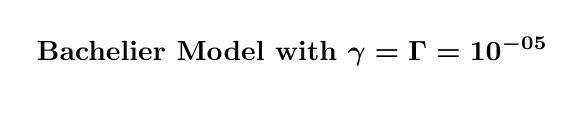
\begin{tikzpicture}[%
font=\footnotesize
]

\begin{axis}[%
width=0.951\figwidth,
height=\figheight,
at={(0\figwidth,0\figheight)},
scale only axis,
xmin=0,
xmax=3,
tick align=outside,
xlabel={$\bar P - p$},
xmajorgrids,
ymin=0,
ymax=1,
ylabel={$T-t$},
ymajorgrids,
zmin=0,
zmax=0.02,
zlabel={Optimal Rate $\bar u$},
zmajorgrids,
view={50}{40},
axis background/.style={fill=white},
title style={font=\bfseries},
title={Bachelier Model with $\boldsymbol{\gamma = \Gamma = 10^{-05}}$},
axis x line*=bottom,
axis y line*=left,
axis z line*=left
]

\addplot3[%
surf,
shader=flat corner,draw=black,z buffer=sort,colormap={mymap}{[1pt] rgb(0pt)=(0.2081,0.1663,0.5292); rgb(1pt)=(0.211624,0.189781,0.577676); rgb(2pt)=(0.212252,0.213771,0.626971); rgb(3pt)=(0.2081,0.2386,0.677086); rgb(4pt)=(0.195905,0.264457,0.7279); rgb(5pt)=(0.170729,0.291938,0.779248); rgb(6pt)=(0.125271,0.324243,0.830271); rgb(7pt)=(0.0591333,0.359833,0.868333); rgb(8pt)=(0.0116952,0.38751,0.881957); rgb(9pt)=(0.00595714,0.408614,0.882843); rgb(10pt)=(0.0165143,0.4266,0.878633); rgb(11pt)=(0.0328524,0.443043,0.871957); rgb(12pt)=(0.0498143,0.458571,0.864057); rgb(13pt)=(0.0629333,0.47369,0.855438); rgb(14pt)=(0.0722667,0.488667,0.8467); rgb(15pt)=(0.0779429,0.503986,0.838371); rgb(16pt)=(0.0793476,0.520024,0.831181); rgb(17pt)=(0.0749429,0.537543,0.826271); rgb(18pt)=(0.0640571,0.556986,0.823957); rgb(19pt)=(0.0487714,0.577224,0.822829); rgb(20pt)=(0.0343429,0.596581,0.819852); rgb(21pt)=(0.0265,0.6137,0.8135); rgb(22pt)=(0.0238905,0.628662,0.803762); rgb(23pt)=(0.0230905,0.641786,0.791267); rgb(24pt)=(0.0227714,0.653486,0.776757); rgb(25pt)=(0.0266619,0.664195,0.760719); rgb(26pt)=(0.0383714,0.674271,0.743552); rgb(27pt)=(0.0589714,0.683757,0.725386); rgb(28pt)=(0.0843,0.692833,0.706167); rgb(29pt)=(0.113295,0.7015,0.685857); rgb(30pt)=(0.145271,0.709757,0.664629); rgb(31pt)=(0.180133,0.717657,0.642433); rgb(32pt)=(0.217829,0.725043,0.619262); rgb(33pt)=(0.258643,0.731714,0.595429); rgb(34pt)=(0.302171,0.737605,0.571186); rgb(35pt)=(0.348167,0.742433,0.547267); rgb(36pt)=(0.395257,0.7459,0.524443); rgb(37pt)=(0.44201,0.748081,0.503314); rgb(38pt)=(0.487124,0.749062,0.483976); rgb(39pt)=(0.530029,0.749114,0.466114); rgb(40pt)=(0.570857,0.748519,0.44939); rgb(41pt)=(0.609852,0.747314,0.433686); rgb(42pt)=(0.6473,0.7456,0.4188); rgb(43pt)=(0.683419,0.743476,0.404433); rgb(44pt)=(0.71841,0.741133,0.390476); rgb(45pt)=(0.752486,0.7384,0.376814); rgb(46pt)=(0.785843,0.735567,0.363271); rgb(47pt)=(0.818505,0.732733,0.34979); rgb(48pt)=(0.850657,0.7299,0.336029); rgb(49pt)=(0.882433,0.727433,0.3217); rgb(50pt)=(0.913933,0.725786,0.306276); rgb(51pt)=(0.944957,0.726114,0.288643); rgb(52pt)=(0.973895,0.731395,0.266648); rgb(53pt)=(0.993771,0.745457,0.240348); rgb(54pt)=(0.999043,0.765314,0.216414); rgb(55pt)=(0.995533,0.786057,0.196652); rgb(56pt)=(0.988,0.8066,0.179367); rgb(57pt)=(0.978857,0.827143,0.163314); rgb(58pt)=(0.9697,0.848138,0.147452); rgb(59pt)=(0.962586,0.870514,0.1309); rgb(60pt)=(0.958871,0.8949,0.113243); rgb(61pt)=(0.959824,0.921833,0.0948381); rgb(62pt)=(0.9661,0.951443,0.0755333); rgb(63pt)=(0.9763,0.9831,0.0538)},mesh/rows=25]
table[row sep=crcr, point meta=\thisrow{c}] {%
%
x	y	z	c\\
0	0.01	0.00199572273713903	0.00199572273713903\\
0	0.0302040816326531	0.00346771034751481	0.00346771034751481\\
0	0.0504081632653061	0.00447954439749076	0.00447954439749076\\
0	0.0706122448979592	0.00530163582180342	0.00530163582180342\\
0	0.0908163265306122	0.00601234040790398	0.00601234040790398\\
0	0.111020408163265	0.00664748595695432	0.00664748595695432\\
0	0.131224489795918	0.00722702404308809	0.00722702404308809\\
0	0.151428571428571	0.00776341942115802	0.00776341942115802\\
0	0.171632653061224	0.00826507706145086	0.00826507706145086\\
0	0.191836734693878	0.00873798265020432	0.00873798265020432\\
0	0.212040816326531	0.00918657799900098	0.00918657799900098\\
0	0.232244897959184	0.0096142669472589	0.0096142669472589\\
0	0.252448979591837	0.0100237261944078	0.0100237261944078\\
0	0.27265306122449	0.010417105802798	0.010417105802798\\
0	0.292857142857143	0.0107961637649053	0.0107961637649053\\
0	0.313061224489796	0.011162359345712	0.011162359345712\\
0	0.333265306122449	0.0115169196594616	0.0115169196594616\\
0	0.353469387755102	0.0118608883032705	0.0118608883032705\\
0	0.373673469387755	0.0121951616263302	0.0121951616263302\\
0	0.393877551020408	0.0125205162725683	0.0125205162725683\\
0	0.414081632653061	0.0128376304335369	0.0128376304335369\\
0	0.434285714285714	0.0131471004827608	0.0131471004827608\\
0	0.454489795918367	0.0134494541620795	0.0134494541620795\\
0	0.47469387755102	0.0137451611552344	0.0137451611552344\\
0	0.494897959183673	0.014034641654894	0.014034641654894\\
0	0.515102040816326	0.0143182733697878	0.0143182733697878\\
0	0.53530612244898	0.0145963973056339	0.0145963973056339\\
0	0.555510204081633	0.0148693225723925	0.0148693225723925\\
0	0.575714285714286	0.0151373304110121	0.0151373304110121\\
0	0.595918367346939	0.0154006775892858	0.0154006775892858\\
0	0.616122448979592	0.015659599283449	0.015659599283449\\
0	0.636326530612245	0.0159143115377566	0.0159143115377566\\
0	0.656530612244898	0.0161650133750778	0.0161650133750778\\
0	0.676734693877551	0.0164118886172842	0.0164118886172842\\
0	0.696938775510204	0.0166551074627046	0.0166551074627046\\
0	0.717142857142857	0.0168948278591579	0.0168948278591579\\
0	0.73734693877551	0.0171311967040272	0.0171311967040272\\
0	0.757551020408163	0.0173643508972977	0.0173643508972977\\
0	0.777755102040816	0.0175944182689634	0.0175944182689634\\
0	0.797959183673469	0.0178215183986895	0.0178215183986895\\
0	0.818163265306122	0.0180457633426177	0.0180457633426177\\
0	0.838367346938775	0.0182672582798648	0.0182672582798648\\
0	0.858571428571429	0.0184861020893149	0.0184861020893149\\
0	0.878775510204082	0.0187023878656308	0.0187023878656308\\
0	0.898979591836735	0.0189162033822176	0.0189162033822176\\
0	0.919183673469388	0.0191276315075457	0.0191276315075457\\
0	0.939387755102041	0.019336750580568	0.019336750580568\\
0	0.959591836734694	0.0195436347499332	0.0195436347499332\\
0	0.979795918367347	0.019748354281248	0.019748354281248\\
0	1	0.0199509758359535	0.0199509758359535\\
0.125	0.01	1.10306875862005e-05	1.10306875862005e-05\\
0.125	0.0302040816326531	0.000293599723320286	0.000293599723320286\\
0.125	0.0504081632653061	0.00075103030670134	0.00075103030670134\\
0.125	0.0706122448979592	0.00123856664368105	0.00123856664368105\\
0.125	0.0908163265306122	0.0017198349786484	0.0017198349786484\\
0.125	0.111020408163265	0.00218518813914589	0.00218518813914589\\
0.125	0.131224489795918	0.00263256424403462	0.00263256424403462\\
0.125	0.151428571428571	0.0030623212763881	0.0030623212763881\\
0.125	0.171632653061224	0.0034755871890253	0.0034755871890253\\
0.125	0.191836734693878	0.00387367729207821	0.00387367729207821\\
0.125	0.212040816326531	0.0042578808783809	0.0042578808783809\\
0.125	0.232244897959184	0.00462938687228723	0.00462938687228723\\
0.125	0.252448979591837	0.00498926425669762	0.00498926425669762\\
0.125	0.27265306122449	0.00533846412610116	0.00533846412610116\\
0.125	0.292857142857143	0.00567782970099822	0.00567782970099822\\
0.125	0.313061224489796	0.00600810855933179	0.00600810855933179\\
0.125	0.333265306122449	0.00632996470664398	0.00632996470664398\\
0.125	0.353469387755102	0.00664398957570265	0.00664398957570265\\
0.125	0.373673469387755	0.00695071169101388	0.00695071169101388\\
0.125	0.393877551020408	0.00725060500954026	0.00725060500954026\\
0.125	0.414081632653061	0.00754409605743482	0.00754409605743482\\
0.125	0.434285714285714	0.00783157001533475	0.00783157001533475\\
0.125	0.454489795918367	0.00811337590426676	0.00811337590426676\\
0.125	0.47469387755102	0.00838983101036795	0.00838983101036795\\
0.125	0.494897959183673	0.00866122467062302	0.00866122467062302\\
0.125	0.515102040816326	0.00892782151173479	0.00892782151173479\\
0.125	0.53530612244898	0.00918986424784793	0.00918986424784793\\
0.125	0.555510204081633	0.00944757608853112	0.00944757608853112\\
0.125	0.575714285714286	0.0097011628271885	0.0097011628271885\\
0.125	0.595918367346939	0.00995081465647512	0.00995081465647512\\
0.125	0.616122448979592	0.0101967077482894	0.0101967077482894\\
0.125	0.636326530612245	0.010439005659297	0.010439005659297\\
0.125	0.656530612244898	0.0106778605152265	0.0106778605152265\\
0.125	0.676734693877551	0.010913414107888	0.010913414107888\\
0.125	0.696938775510204	0.0111457988371264	0.0111457988371264\\
0.125	0.717142857142857	0.0113751385280414	0.0113751385280414\\
0.125	0.73734693877551	0.011601549266899	0.011601549266899\\
0.125	0.757551020408163	0.011825139943478	0.011825139943478\\
0.125	0.777755102040816	0.012046012922628	0.012046012922628\\
0.125	0.797959183673469	0.0122642645604035	0.0122642645604035\\
0.125	0.818163265306122	0.0124799856834139	0.0124799856834139\\
0.125	0.838367346938775	0.0126932620204568	0.0126932620204568\\
0.125	0.858571428571429	0.0129041745920674	0.0129041745920674\\
0.125	0.878775510204082	0.0131128000628524	0.0131128000628524\\
0.125	0.898979591836735	0.0133192110608345	0.0133192110608345\\
0.125	0.919183673469388	0.0135234764674801	0.0135234764674801\\
0.125	0.939387755102041	0.0137256616816133	0.0137256616816133\\
0.125	0.959591836734694	0.0139258288600169	0.0139258288600169\\
0.125	0.979795918367347	0.0141240371371755	0.0141240371371755\\
0.125	1	0.0143203428263168	0.0143203428263168\\
0.25	0.01	1.01026731331038e-06	1.01026731331038e-06\\
0.25	0.0302040816326531	6.12437307922703e-06	6.12437307922703e-06\\
0.25	0.0504081632653061	5.18401147621789e-05	5.18401147621789e-05\\
0.25	0.0706122448979592	0.000155109348610919	0.000155109348610919\\
0.25	0.0908163265306122	0.000305284101599257	0.000305284101599257\\
0.25	0.111020408163265	0.00048867826850651	0.00048867826850651\\
0.25	0.131224489795918	0.000694683286014349	0.000694683286014349\\
0.25	0.151428571428571	0.000915830510571455	0.000915830510571455\\
0.25	0.171632653061224	0.00114695734135227	0.00114695734135227\\
0.25	0.191836734693878	0.00138448229364414	0.00138448229364414\\
0.25	0.212040816326531	0.00162589610880191	0.00162589610880191\\
0.25	0.232244897959184	0.00186942177300387	0.00186942177300387\\
0.25	0.252448979591837	0.00211378883091824	0.00211378883091824\\
0.25	0.27265306122449	0.00235808232058585	0.00235808232058585\\
0.25	0.292857142857143	0.00260164027739888	0.00260164027739888\\
0.25	0.313061224489796	0.00284398313569312	0.00284398313569312\\
0.25	0.333265306122449	0.00308476436538434	0.00308476436538434\\
0.25	0.353469387755102	0.0033237354598758	0.0033237354598758\\
0.25	0.373673469387755	0.00356072077111441	0.00356072077111441\\
0.25	0.393877551020408	0.00379559920076026	0.00379559920076026\\
0.25	0.414081632653061	0.00402829073124887	0.00402829073124887\\
0.25	0.434285714285714	0.00425874641769099	0.00425874641769099\\
0.25	0.454489795918367	0.00448694088417545	0.00448694088417545\\
0.25	0.47469387755102	0.00471286665241016	0.00471286665241016\\
0.25	0.494897959183673	0.004936529824635	0.004936529824635\\
0.25	0.515102040816326	0.00515794677682901	0.00515794677682901\\
0.25	0.53530612244898	0.00537714161206564	0.00537714161206564\\
0.25	0.555510204081633	0.00559414419029517	0.00559414419029517\\
0.25	0.575714285714286	0.00580898859837284	0.00580898859837284\\
0.25	0.595918367346939	0.00602171195852195	0.00602171195852195\\
0.25	0.616122448979592	0.00623235349851042	0.00623235349851042\\
0.25	0.636326530612245	0.00644095382529727	0.00644095382529727\\
0.25	0.656530612244898	0.00664755435762909	0.00664755435762909\\
0.25	0.676734693877551	0.00685219688333992	0.00685219688333992\\
0.25	0.696938775510204	0.00705492321485408	0.00705492321485408\\
0.25	0.717142857142857	0.00725577492227436	0.00725577492227436\\
0.25	0.73734693877551	0.00745479312793295	0.00745479312793295\\
0.25	0.757551020408163	0.00765201834973902	0.00765201834973902\\
0.25	0.777755102040816	0.00784749038333022	0.00784749038333022\\
0.25	0.797959183673469	0.00804124821511279	0.00804124821511279\\
0.25	0.818163265306122	0.008233329959899	0.008233329959899\\
0.25	0.838367346938775	0.008423772818125	0.008423772818125\\
0.25	0.858571428571429	0.00861261304863715	0.00861261304863715\\
0.25	0.878775510204082	0.00879988595383049	0.00879988595383049\\
0.25	0.898979591836735	0.00898562587455527	0.00898562587455527\\
0.25	0.919183673469388	0.00916986619271165	0.00916986619271165\\
0.25	0.939387755102041	0.00935263933985647	0.00935263933985647\\
0.25	0.959591836734694	0.00953397681046937	0.00953397681046937\\
0.25	0.979795918367347	0.00971390917878684	0.00971390917878684\\
0.25	1	0.00989246611832247	0.00989246611832247\\
0.375	0.01	1.01000000503724e-06	1.01000000503724e-06\\
0.375	0.0302040816326531	1.04485467470845e-06	1.04485467470845e-06\\
0.375	0.0504081632653061	2.27452775653183e-06	2.27452775653183e-06\\
0.375	0.0706122448979592	1.04476227321461e-05	1.04476227321461e-05\\
0.375	0.0908163265306122	3.23595379271355e-05	3.23595379271355e-05\\
0.375	0.111020408163265	7.14719068131642e-05	7.14719068131642e-05\\
0.375	0.131224489795918	0.000128223316200038	0.000128223316200038\\
0.375	0.151428571428571	0.000201431077742383	0.000201431077742383\\
0.375	0.171632653061224	0.000289268967441192	0.000289268967441192\\
0.375	0.191836734693878	0.000389780945788812	0.000389780945788812\\
0.375	0.212040816326531	0.00050111524998755	0.00050111524998755\\
0.375	0.232244897959184	0.000621614239267901	0.000621614239267901\\
0.375	0.252448979591837	0.000749835322113033	0.000749835322113033\\
0.375	0.27265306122449	0.000884541337995216	0.000884541337995216\\
0.375	0.292857142857143	0.00102467912553479	0.00102467912553479\\
0.375	0.313061224489796	0.00116935508747273	0.00116935508747273\\
0.375	0.333265306122449	0.00131781166473716	0.00131781166473716\\
0.375	0.353469387755102	0.00146940625711113	0.00146940625711113\\
0.375	0.373673469387755	0.00162359300702328	0.00162359300702328\\
0.375	0.393877551020408	0.00177990736051329	0.00177990736051329\\
0.375	0.414081632653061	0.00193795311858261	0.00193795311858261\\
0.375	0.434285714285714	0.00209739163493247	0.00209739163493247\\
0.375	0.454489795918367	0.00225793282397538	0.00225793282397538\\
0.375	0.47469387755102	0.00241932767732876	0.00241932767732876\\
0.375	0.494897959183673	0.00258136202917208	0.00258136202917208\\
0.375	0.515102040816326	0.00274385135235581	0.00274385135235581\\
0.375	0.53530612244898	0.00290663640448192	0.00290663640448192\\
0.375	0.555510204081633	0.00306957957525154	0.00306957957525154\\
0.375	0.575714285714286	0.00323256181324096	0.00323256181324096\\
0.375	0.595918367346939	0.00339548003243645	0.00339548003243645\\
0.375	0.616122448979592	0.00355824491699604	0.00355824491699604\\
0.375	0.636326530612245	0.00372077905747439	0.00372077905747439\\
0.375	0.656530612244898	0.00388301536374519	0.00388301536374519\\
0.375	0.676734693877551	0.00404489570959769	0.00404489570959769\\
0.375	0.696938775510204	0.00420636977189847	0.00420636977189847\\
0.375	0.717142857142857	0.00436739403364926	0.00436739403364926\\
0.375	0.73734693877551	0.0045279309255199	0.0045279309255199\\
0.375	0.757551020408163	0.00468794808472389	0.00468794808472389\\
0.375	0.777755102040816	0.00484741771361632	0.00484741771361632\\
0.375	0.797959183673469	0.00500631602327865	0.00500631602327865\\
0.375	0.818163265306122	0.00516462274973066	0.00516462274973066\\
0.375	0.838367346938775	0.00532232073237293	0.00532232073237293\\
0.375	0.858571428571429	0.00547939554588844	0.00547939554588844\\
0.375	0.878775510204082	0.00563583517818339	0.00563583517818339\\
0.375	0.898979591836735	0.00579162974807239	0.00579162974807239\\
0.375	0.919183673469388	0.0059467712573541	0.0059467712573541\\
0.375	0.939387755102041	0.00610125337271151	0.00610125337271151\\
0.375	0.959591836734694	0.00625507123353324	0.00625507123353324\\
0.375	0.979795918367347	0.0064082212823104	0.0064082212823104\\
0.375	1	0.00656070111473506	0.00656070111473506\\
0.5	0.01	1.01000000501667e-06	1.01000000501667e-06\\
0.5	0.0302040816326531	1.03021036215418e-06	1.03021036215418e-06\\
0.5	0.0504081632653061	1.06015988591143e-06	1.06015988591143e-06\\
0.5	0.0706122448979592	1.33490760843779e-06	1.33490760843779e-06\\
0.5	0.0908163265306122	2.87933090779131e-06	2.87933090779131e-06\\
0.5	0.111020408163265	7.45016979844545e-06	7.45016979844545e-06\\
0.5	0.131224489795918	1.68589310382665e-05	1.68589310382665e-05\\
0.5	0.151428571428571	3.24986307199888e-05	3.24986307199888e-05\\
0.5	0.171632653061224	5.52253466100567e-05	5.52253466100567e-05\\
0.5	0.191836734693878	8.54262572618395e-05	8.54262572618395e-05\\
0.5	0.212040816326531	0.000123140347480908	0.000123140347480908\\
0.5	0.232244897959184	0.000168172145555304	0.000168172145555304\\
0.5	0.252448979591837	0.000220180832082117	0.000220180832082117\\
0.5	0.27265306122449	0.00027874421514171	0.00027874421514171\\
0.5	0.292857142857143	0.000343402318162617	0.000343402318162617\\
0.5	0.313061224489796	0.000413685924982823	0.000413685924982823\\
0.5	0.333265306122449	0.000489134559259304	0.000489134559259304\\
0.5	0.353469387755102	0.000569307261710809	0.000569307261710809\\
0.5	0.373673469387755	0.000653788562591981	0.000653788562591981\\
0.5	0.393877551020408	0.000742191309553218	0.000742191309553218\\
0.5	0.414081632653061	0.000834157480525773	0.000834157480525773\\
0.5	0.434285714285714	0.000929357741058673	0.000929357741058673\\
0.5	0.454489795918367	0.00102749025158822	0.00102749025158822\\
0.5	0.47469387755102	0.00112827905768955	0.00112827905768955\\
0.5	0.494897959183673	0.00123147228003985	0.00123147228003985\\
0.5	0.515102040816326	0.00133684024274044	0.00133684024274044\\
0.5	0.53530612244898	0.00144417362647445	0.00144417362647445\\
0.5	0.555510204081633	0.00155328169831421	0.00155328169831421\\
0.5	0.575714285714286	0.00166399064713425	0.00166399064713425\\
0.5	0.595918367346939	0.00177614203867675	0.00177614203867675\\
0.5	0.616122448979592	0.00188959139474803	0.00188959139474803\\
0.5	0.636326530612245	0.00200420689503455	0.00200420689503455\\
0.5	0.656530612244898	0.00211986819642374	0.00211986819642374\\
0.5	0.676734693877551	0.00223646536269139	0.00223646536269139\\
0.5	0.696938775510204	0.0023538978964292	0.0023538978964292\\
0.5	0.717142857142857	0.00247207386476483	0.00247207386476483\\
0.5	0.73734693877551	0.00259090911052486	0.00259090911052486\\
0.5	0.757551020408163	0.00271032654084235	0.00271032654084235\\
0.5	0.777755102040816	0.00283025548570451	0.00283025548570451\\
0.5	0.797959183673469	0.00295063111950031	0.00295063111950031\\
0.5	0.818163265306122	0.00307139393921436	0.00307139393921436\\
0.5	0.838367346938775	0.00319248929349407	0.00319248929349407\\
0.5	0.858571428571429	0.00331386695737258	0.00331386695737258\\
0.5	0.878775510204082	0.00343548074795066	0.00343548074795066\\
0.5	0.898979591836735	0.00355728817682181	0.00355728817682181\\
0.5	0.919183673469388	0.00367925013546432	0.00367925013546432\\
0.5	0.939387755102041	0.00380133061022243	0.00380133061022243\\
0.5	0.959591836734694	0.00392349642385788	0.00392349642385788\\
0.5	0.979795918367347	0.00404571700097592	0.00404571700097592\\
0.5	1	0.00416796415491795	0.00416796415491795\\
0.625	0.01	1.01000000501667e-06	1.01000000501667e-06\\
0.625	0.0302040816326531	1.03020412807704e-06	1.03020412807704e-06\\
0.625	0.0504081632653061	1.05043288669953e-06	1.05043288669953e-06\\
0.625	0.0706122448979592	1.0739452880784e-06	1.0739452880784e-06\\
0.625	0.0908163265306122	1.14615232799027e-06	1.14615232799027e-06\\
0.625	0.111020408163265	1.45914359058141e-06	1.45914359058141e-06\\
0.625	0.131224489795918	2.41873055440506e-06	2.41873055440506e-06\\
0.625	0.151428571428571	4.59573180552037e-06	4.59573180552037e-06\\
0.625	0.171632653061224	8.6190111274569e-06	8.6190111274569e-06\\
0.625	0.191836734693878	1.50811883288309e-05	1.50811883288309e-05\\
0.625	0.212040816326531	2.44824064239706e-05	2.44824064239706e-05\\
0.625	0.232244897959184	3.72082794999214e-05	3.72082794999214e-05\\
0.625	0.252448979591837	5.35300689060466e-05	5.35300689060466e-05\\
0.625	0.27265306122449	7.36165145655193e-05	7.36165145655193e-05\\
0.625	0.292857142857143	9.75502715729534e-05	9.75502715729534e-05\\
0.625	0.313061224489796	0.000125344930569061	0.000125344930569061\\
0.625	0.333265306122449	0.000156960629758282	0.000156960629758282\\
0.625	0.353469387755102	0.000192317465413386	0.000192317465413386\\
0.625	0.373673469387755	0.000231306552035317	0.000231306552035317\\
0.625	0.393877551020408	0.000273798894629972	0.000273798894629972\\
0.625	0.414081632653061	0.000319652360813197	0.000319652360813197\\
0.625	0.434285714285714	0.000368717068551157	0.000368717068551157\\
0.625	0.454489795918367	0.000420839486981697	0.000420839486981697\\
0.625	0.47469387755102	0.000475865510486114	0.000475865510486114\\
0.625	0.494897959183673	0.000533642724174791	0.000533642724174791\\
0.625	0.515102040816326	0.000594022038976665	0.000594022038976665\\
0.625	0.53530612244898	0.000656858839368178	0.000656858839368178\\
0.625	0.555510204081633	0.000722013757194173	0.000722013757194173\\
0.625	0.575714285714286	0.000789353160802458	0.000789353160802458\\
0.625	0.595918367346939	0.000858749429212026	0.000858749429212026\\
0.625	0.616122448979592	0.000930081065523073	0.000930081065523073\\
0.625	0.636326530612245	0.00100323269153824	0.00100323269153824\\
0.625	0.656530612244898	0.00107809495596312	0.00107809495596312\\
0.625	0.676734693877551	0.00115456438105235	0.00115456438105235\\
0.625	0.696938775510204	0.00123254316672396	0.00123254316672396\\
0.625	0.717142857142857	0.00131193896662364	0.00131193896662364\\
0.625	0.73734693877551	0.00139266464709776	0.00139266464709776\\
0.625	0.757551020408163	0.00147463803730764	0.00147463803730764\\
0.625	0.777755102040816	0.00155778167660925	0.00155778167660925\\
0.625	0.797959183673469	0.00164202256369782	0.00164202256369782\\
0.625	0.818163265306122	0.00172729191076577	0.00172729191076577\\
0.625	0.838367346938775	0.00181352490496364	0.00181352490496364\\
0.625	0.858571428571429	0.00190066047872029	0.00190066047872029\\
0.625	0.878775510204082	0.00198864108992156	0.00198864108992156\\
0.625	0.898979591836735	0.00207741251252499	0.00207741251252499\\
0.625	0.919183673469388	0.00216692363787299	0.00216692363787299\\
0.625	0.939387755102041	0.00225712628673194	0.00225712628673194\\
0.625	0.959591836734694	0.0023479750319144	0.0023479750319144\\
0.625	0.979795918367347	0.00243942703121842	0.00243942703121842\\
0.625	1	0.00253144187033301	0.00253144187033301\\
0.75	0.01	1.01000000501667e-06	1.01000000501667e-06\\
0.75	0.0302040816326531	1.03020412770623e-06	1.03020412770623e-06\\
0.75	0.0504081632653061	1.05040831158137e-06	1.05040831158137e-06\\
0.75	0.0706122448979592	1.07063089412924e-06	1.07063089412924e-06\\
0.75	0.0908163265306122	1.0917254868516e-06	1.0917254868516e-06\\
0.75	0.111020408163265	1.12248295099822e-06	1.12248295099822e-06\\
0.75	0.131224489795918	1.19993391475135e-06	1.19993391475135e-06\\
0.75	0.151428571428571	1.41364128493373e-06	1.41364128493373e-06\\
0.75	0.171632653061224	1.91624936310066e-06	1.91624936310066e-06\\
0.75	0.191836734693878	2.91525626397535e-06	2.91525626397535e-06\\
0.75	0.212040816326531	4.65316055935226e-06	4.65316055935226e-06\\
0.75	0.232244897959184	7.38509264372399e-06	7.38509264372399e-06\\
0.75	0.252448979591837	1.13597179837916e-05	1.13597179837916e-05\\
0.75	0.27265306122449	1.68055973858948e-05	1.68055973858948e-05\\
0.75	0.292857142857143	2.39229570999472e-05	2.39229570999472e-05\\
0.75	0.313061224489796	3.2879850865002e-05	3.2879850865002e-05\\
0.75	0.333265306122449	4.38114811016904e-05	4.38114811016904e-05\\
0.75	0.353469387755102	5.68215797142798e-05	5.68215797142798e-05\\
0.75	0.373673469387755	7.19849938807952e-05	7.19849938807952e-05\\
0.75	0.393877551020408	8.93508667450671e-05	8.93508667450671e-05\\
0.75	0.414081632653061	0.00010894600528017	0.00010894600528017\\
0.75	0.434285714285714	0.000130778179747088	0.000130778179747088\\
0.75	0.454489795918367	0.000154839206771498	0.000154839206771498\\
0.75	0.47469387755102	0.000181107740663822	0.000181107740663822\\
0.75	0.494897959183673	0.000209551744536378	0.000209551744536378\\
0.75	0.515102040816326	0.000240130641698985	0.000240130641698985\\
0.75	0.53530612244898	0.000272797164549455	0.000272797164549455\\
0.75	0.555510204081633	0.000307498926901287	0.000307498926901287\\
0.75	0.575714285714286	0.00034417974931953	0.00034417974931953\\
0.75	0.595918367346939	0.000382780767542396	0.000382780767542396\\
0.75	0.616122448979592	0.000423241352760045	0.000423241352760045\\
0.75	0.636326530612245	0.000465499870252152	0.000465499870252152\\
0.75	0.656530612244898	0.00050949430018893	0.00050949430018893\\
0.75	0.676734693877551	0.000555162741604433	0.000555162741604433\\
0.75	0.696938775510204	0.00060244381784801	0.00060244381784801\\
0.75	0.717142857142857	0.000651276999313182	0.000651276999313182\\
0.75	0.73734693877551	0.000701602856981216	0.000701602856981216\\
0.75	0.757551020408163	0.000753363258313339	0.000753363258313339\\
0.75	0.777755102040816	0.000806501515275029	0.000806501515275029\\
0.75	0.797959183673469	0.000860962492761277	0.000860962492761277\\
0.75	0.818163265306122	0.000916692684391076	0.000916692684391076\\
0.75	0.838367346938775	0.000973640261528706	0.000973640261528706\\
0.75	0.858571428571429	0.00103175510044506	0.00103175510044506\\
0.75	0.878775510204082	0.0010909887917321	0.0010909887917321\\
0.75	0.898979591836735	0.0011512946354072	0.0011512946354072\\
0.75	0.919183673469388	0.00121262762457401	0.00121262762457401\\
0.75	0.939387755102041	0.00127494442002618	0.00127494442002618\\
0.75	0.959591836734694	0.00133820331777668	0.00133820331777668\\
0.75	0.979795918367347	0.00140236421115644	0.00140236421115644\\
0.75	1	0.00146738854884178	0.00146738854884178\\
0.875	0.01	1.01000000501667e-06	1.01000000501667e-06\\
0.875	0.0302040816326531	1.03020412770623e-06	1.03020412770623e-06\\
0.875	0.0504081632653061	1.05040829245374e-06	1.05040829245374e-06\\
0.875	0.0706122448979592	1.07061254386113e-06	1.07061254386113e-06\\
0.875	0.0908163265306122	1.09082457096857e-06	1.09082457096857e-06\\
0.875	0.111020408163265	1.11124469861652e-06	1.11124469861652e-06\\
0.875	0.131224489795918	1.13359072731421e-06	1.13359072731421e-06\\
0.875	0.151428571428571	1.16512893751044e-06	1.16512893751044e-06\\
0.875	0.171632653061224	1.225188748233e-06	1.225188748233e-06\\
0.875	0.191836734693878	1.35146148627446e-06	1.35146148627446e-06\\
0.875	0.212040816326531	1.60336066002846e-06	1.60336066002846e-06\\
0.875	0.232244897959184	2.06154239436943e-06	2.06154239436943e-06\\
0.875	0.252448979591837	2.82431709888188e-06	2.82431709888188e-06\\
0.875	0.27265306122449	4.00233155544458e-06	4.00233155544458e-06\\
0.875	0.292857142857143	5.71280291511013e-06	5.71280291511013e-06\\
0.875	0.313061224489796	8.0741862999485e-06	8.0741862999485e-06\\
0.875	0.333265306122449	1.12017448248827e-05	1.12017448248827e-05\\
0.875	0.353469387755102	1.52041805009696e-05	1.52041805009696e-05\\
0.875	0.373673469387755	2.0181291961301e-05	2.0181291961301e-05\\
0.875	0.393877551020408	2.62225261475344e-05	2.62225261475344e-05\\
0.875	0.414081632653061	3.34062546924622e-05	3.34062546924622e-05\\
0.875	0.434285714285714	4.17996056815891e-05	4.17996056815891e-05\\
0.875	0.454489795918367	5.14586996691333e-05	5.14586996691333e-05\\
0.875	0.47469387755102	6.2429164038903e-05	6.2429164038903e-05\\
0.875	0.494897959183673	7.47468257481497e-05	7.47468257481497e-05\\
0.875	0.515102040816326	8.84385060564245e-05	8.84385060564245e-05\\
0.875	0.53530612244898	0.000103522860787717	0.000103522860787717\\
0.875	0.555510204081633	0.000120011225798724	0.000120011225798724\\
0.875	0.575714285714286	0.000137908439931648	0.000137908439931648\\
0.875	0.595918367346939	0.000157213627324092	0.000157213627324092\\
0.875	0.616122448979592	0.000177920928081326	0.000177920928081326\\
0.875	0.636326530612245	0.00020002017149991	0.00020002017149991\\
0.875	0.656530612244898	0.000223497489708693	0.000223497489708693\\
0.875	0.676734693877551	0.000248335872127793	0.000248335872127793\\
0.875	0.696938775510204	0.000274515662828979	0.000274515662828979\\
0.875	0.717142857142857	0.000302015003938972	0.000302015003938972\\
0.875	0.73734693877551	0.000330810228834347	0.000330810228834347\\
0.875	0.757551020408163	0.000360876209164599	0.000360876209164599\\
0.875	0.777755102040816	0.000392186659806687	0.000392186659806687\\
0.875	0.797959183673469	0.000424714405772329	0.000424714405772329\\
0.875	0.818163265306122	0.000458431614911466	0.000458431614911466\\
0.875	0.838367346938775	0.000493310000019479	0.000493310000019479\\
0.875	0.858571428571429	0.000529320993689012	0.000529320993689012\\
0.875	0.878775510204082	0.000566435898968334	0.000566435898968334\\
0.875	0.898979591836735	0.000604626018609864	0.000604626018609864\\
0.875	0.919183673469388	0.000643862765423126	0.000643862765423126\\
0.875	0.939387755102041	0.000684117755991338	0.000684117755991338\\
0.875	0.959591836734694	0.000725362889772944	0.000725362889772944\\
0.875	0.979795918367347	0.000767570415390272	0.000767570415390272\\
0.875	1	0.000810712985707382	0.000810712985707382\\
1	0.01	1.01000000501667e-06	1.01000000501667e-06\\
1	0.0302040816326531	1.03020412770623e-06	1.03020412770623e-06\\
1	0.0504081632653061	1.05040829244923e-06	1.05040829244923e-06\\
1	0.0706122448979592	1.07061250011493e-06	1.07061250011493e-06\\
1	0.0908163265306122	1.09081678633313e-06	1.09081678633313e-06\\
1	0.111020408163265	1.11102361215877e-06	1.11102361215877e-06\\
1	0.131224489795918	1.13127751715227e-06	1.13127751715227e-06\\
1	0.151428571428571	1.15191747625936e-06	1.15191747625936e-06\\
1	0.171632653061224	1.17438676599552e-06	1.17438676599552e-06\\
1	0.191836734693878	1.20280659213484e-06	1.20280659213484e-06\\
1	0.212040816326531	1.24606744583818e-06	1.24606744583818e-06\\
1	0.232244897959184	1.3198585382257e-06	1.3198585382257e-06\\
1	0.252448979591837	1.44808446863574e-06	1.44808446863574e-06\\
1	0.27265306122449	1.66338482259818e-06	1.66338482259818e-06\\
1	0.292857142857143	2.00675860473829e-06	2.00675860473829e-06\\
1	0.313061224489796	2.52648114781192e-06	2.52648114781192e-06\\
1	0.333265306122449	3.27657151092845e-06	3.27657151092845e-06\\
1	0.353469387755102	4.31505775051632e-06	4.31505775051632e-06\\
1	0.373673469387755	5.70223655362704e-06	5.70223655362704e-06\\
1	0.393877551020408	7.49906216035814e-06	7.49906216035814e-06\\
1	0.414081632653061	9.76574359217232e-06	9.76574359217232e-06\\
1	0.434285714285714	1.25605854867928e-05	1.25605854867928e-05\\
1	0.454489795918367	1.59390771788786e-05	1.59390771788786e-05\\
1	0.47469387755102	1.99532152704402e-05	1.99532152704402e-05\\
1	0.494897959183673	2.46510341802512e-05	2.46510341802512e-05\\
1	0.515102040816326	3.00763144971467e-05	3.00763144971467e-05\\
1	0.53530612244898	3.62684382799638e-05	3.62684382799638e-05\\
1	0.555510204081633	4.3262362159423e-05	4.3262362159423e-05\\
1	0.575714285714286	5.10886820864391e-05	5.10886820864391e-05\\
1	0.595918367346939	5.97737670939074e-05	5.97737670939074e-05\\
1	0.616122448979592	6.93399430294378e-05	6.93399430294378e-05\\
1	0.636326530612245	7.9805710604298e-05	7.9805710604298e-05\\
1	0.656530612244898	9.11859851493226e-05	9.11859851493226e-05\\
1	0.676734693877551	0.00010349234811595	0.00010349234811595\\
1	0.696938775510204	0.000116733302605091	0.000116733302605091\\
1	0.717142857142857	0.00013091452707238	0.00013091452707238\\
1	0.73734693877551	0.000146039122884121	0.000146039122884121\\
1	0.757551020408163	0.000162107852628045	0.000162107852628045\\
1	0.777755102040816	0.000179119367061053	0.000179119367061053\\
1	0.797959183673469	0.000197070419343832	0.000197070419343832\\
1	0.818163265306122	0.000215956065806549	0.000215956065806549\\
1	0.838367346938775	0.000235769852943114	0.000235769852943114\\
1	0.858571428571429	0.000256503990671025	0.000256503990671025\\
1	0.878775510204082	0.000278149512142685	0.000278149512142685\\
1	0.898979591836735	0.000300696420571235	0.000300696420571235\\
1	0.919183673469388	0.000324133823654951	0.000324133823654951\\
1	0.939387755102041	0.000348450056261767	0.000348450056261767\\
1	0.959591836734694	0.000373632792079613	0.000373632792079613\\
1	0.979795918367347	0.000399669144957159	0.000399669144957159\\
1	1	0.000426545760659638	0.000426545760659638\\
1.125	0.01	1.01000000501667e-06	1.01000000501667e-06\\
1.125	0.0302040816326531	1.03020412770623e-06	1.03020412770623e-06\\
1.125	0.0504081632653061	1.05040829244923e-06	1.05040829244923e-06\\
1.125	0.0706122448979592	1.07061250007043e-06	1.07061250007043e-06\\
1.125	0.0908163265306122	1.09081675147505e-06	1.09081675147505e-06\\
1.125	0.111020408163265	1.11102106443018e-06	1.11102106443018e-06\\
1.125	0.131224489795918	1.13122611975232e-06	1.13122611975232e-06\\
1.125	0.151428571428571	1.1514415442629e-06	1.1514415442629e-06\\
1.125	0.171632653061224	1.17173480559662e-06	1.17173480559662e-06\\
1.125	0.191836734693878	1.19239514209466e-06	1.19239514209466e-06\\
1.125	0.212040816326531	1.21429506140291e-06	1.21429506140291e-06\\
1.125	0.232244897959184	1.23947188519971e-06	1.23947188519971e-06\\
1.125	0.252448979591837	1.27185954458971e-06	1.27185954458971e-06\\
1.125	0.27265306122449	1.31803874948151e-06	1.31803874948151e-06\\
1.125	0.292857142857143	1.3878689981123e-06	1.3878689981123e-06\\
1.125	0.313061224489796	1.49490510191626e-06	1.49490510191626e-06\\
1.125	0.333265306122449	1.65655590575226e-06	1.65655590575226e-06\\
1.125	0.353469387755102	1.89399175850367e-06	1.89399175850367e-06\\
1.125	0.373673469387755	2.23184005540659e-06	2.23184005540659e-06\\
1.125	0.393877551020408	2.69772402797199e-06	2.69772402797199e-06\\
1.125	0.414081632653061	3.3217026456753e-06	3.3217026456753e-06\\
1.125	0.434285714285714	4.13566387344846e-06	4.13566387344846e-06\\
1.125	0.454489795918367	5.17271380300523e-06	5.17271380300523e-06\\
1.125	0.47469387755102	6.46659331663309e-06	6.46659331663309e-06\\
1.125	0.494897959183673	8.05114373944924e-06	8.05114373944924e-06\\
1.125	0.515102040816326	9.95983427750522e-06	9.95983427750522e-06\\
1.125	0.53530612244898	1.22253572146016e-05	1.22253572146016e-05\\
1.125	0.555510204081633	1.48792917926711e-05	1.48792917926711e-05\\
1.125	0.575714285714286	1.79518341994094e-05	1.79518341994094e-05\\
1.125	0.595918367346939	2.1471588841417e-05	2.1471588841417e-05\\
1.125	0.616122448979592	2.54654148019628e-05	2.54654148019628e-05\\
1.125	0.636326530612245	2.99583208127734e-05	2.99583208127734e-05\\
1.125	0.656530612244898	3.49734019965427e-05	3.49734019965427e-05\\
1.125	0.676734693877551	4.05318118939669e-05	4.05318118939669e-05\\
1.125	0.696938775510204	4.66527637495624e-05	4.66527637495624e-05\\
1.125	0.717142857142857	5.33535556020678e-05	5.33535556020678e-05\\
1.125	0.73734693877551	6.06496143428297e-05	6.06496143428297e-05\\
1.125	0.757551020408163	6.85545545252659e-05	6.85545545252659e-05\\
1.125	0.777755102040816	7.70802483019769e-05	7.70802483019769e-05\\
1.125	0.797959183673469	8.62369034164604e-05	8.62369034164604e-05\\
1.125	0.818163265306122	9.60331466748496e-05	9.60331466748496e-05\\
1.125	0.838367346938775	0.000106476110766348	0.000106476110766348\\
1.125	0.858571428571429	0.000117571522689414	0.000117571522689414\\
1.125	0.878775510204082	0.000129323792376902	0.000129323792376902\\
1.125	0.898979591836735	0.000141736100401273	0.000141736100401273\\
1.125	0.919183673469388	0.000154810483885212	0.000154810483885212\\
1.125	0.939387755102041	0.000168547919948438	0.000168547919948438\\
1.125	0.959591836734694	0.000182948406192854	0.000182948406192854\\
1.125	0.979795918367347	0.000198011037869939	0.000198011037869939\\
1.125	1	0.00021373408149065	0.00021373408149065\\
1.25	0.01	1.01000000501667e-06	1.01000000501667e-06\\
1.25	0.0302040816326531	1.03020412770623e-06	1.03020412770623e-06\\
1.25	0.0504081632653061	1.05040829244923e-06	1.05040829244923e-06\\
1.25	0.0706122448979592	1.07061250007041e-06	1.07061250007041e-06\\
1.25	0.0908163265306122	1.09081675139461e-06	1.09081675139461e-06\\
1.25	0.111020408163265	1.11102104731325e-06	1.11102104731325e-06\\
1.25	0.131224489795918	1.13122539495314e-06	1.13122539495314e-06\\
1.25	0.151428571428571	1.15142996753333e-06	1.15142996753333e-06\\
1.25	0.171632653061224	1.17163681425042e-06	1.17163681425042e-06\\
1.25	0.191836734693878	1.19185946109717e-06	1.19185946109717e-06\\
1.25	0.212040816326531	1.21215626984534e-06	1.21215626984534e-06\\
1.25	0.232244897959184	1.23271118079473e-06	1.23271118079473e-06\\
1.25	0.252448979591837	1.25398207992317e-06	1.25398207992317e-06\\
1.25	0.27265306122449	1.27692094620382e-06	1.27692094620382e-06\\
1.25	0.292857142857143	1.30324919190182e-06	1.30324919190182e-06\\
1.25	0.313061224489796	1.33575608129478e-06	1.33575608129478e-06\\
1.25	0.333265306122449	1.37858283028372e-06	1.37858283028372e-06\\
1.25	0.353469387755102	1.4374592854921e-06	1.4374592854921e-06\\
1.25	0.373673469387755	1.51987020659914e-06	1.51987020659914e-06\\
1.25	0.393877551020408	1.63514004210463e-06	1.63514004210463e-06\\
1.25	0.414081632653061	1.79443575176796e-06	1.79443575176796e-06\\
1.25	0.434285714285714	2.0106951975708e-06	2.0106951975708e-06\\
1.25	0.454489795918367	2.29849355912244e-06	2.29849355912244e-06\\
1.25	0.47469387755102	2.67386247718766e-06	2.67386247718766e-06\\
1.25	0.494897959183673	3.15407683446597e-06	3.15407683446597e-06\\
1.25	0.515102040816326	3.7574229296229e-06	3.7574229296229e-06\\
1.25	0.53530612244898	4.50295987926572e-06	4.50295987926572e-06\\
1.25	0.555510204081633	5.41028384183956e-06	5.41028384183956e-06\\
1.25	0.575714285714286	6.49930240463018e-06	6.49930240463018e-06\\
1.25	0.595918367346939	7.7900243986449e-06	7.7900243986449e-06\\
1.25	0.616122448979592	9.30236860478082e-06	9.30236860478082e-06\\
1.25	0.636326530612245	1.10559933247802e-05	1.10559933247802e-05\\
1.25	0.656530612244898	1.30701476086679e-05	1.30701476086679e-05\\
1.25	0.676734693877551	1.53635440304274e-05	1.53635440304274e-05\\
1.25	0.696938775510204	1.79542522482357e-05	1.79542522482357e-05\\
1.25	0.717142857142857	2.08596121338254e-05	2.08596121338254e-05\\
1.25	0.73734693877551	2.40961649678606e-05	2.40961649678606e-05\\
1.25	0.757551020408163	2.76796010387238e-05	2.76796010387238e-05\\
1.25	0.777755102040816	3.16247219198038e-05	3.16247219198038e-05\\
1.25	0.797959183673469	3.5945415709372e-05	3.5945415709372e-05\\
1.25	0.818163265306122	4.06546435764524e-05	4.06546435764524e-05\\
1.25	0.838367346938775	4.57644360491038e-05	4.57644360491038e-05\\
1.25	0.858571428571429	5.1285897595401e-05	5.1285897595401e-05\\
1.25	0.878775510204082	5.72292181724034e-05	5.72292181724034e-05\\
1.25	0.898979591836735	6.36036905473785e-05	6.36036905473785e-05\\
1.25	0.919183673469388	7.0417732323371e-05	7.0417732323371e-05\\
1.25	0.939387755102041	7.76789117243488e-05	7.76789117243488e-05\\
1.25	0.959591836734694	8.53939763112929e-05	8.53939763112929e-05\\
1.25	0.979795918367347	9.35688839083475e-05	9.35688839083475e-05\\
1.25	1	0.000102208835116798	0.000102208835116798\\
1.375	0.01	1.01000000501667e-06	1.01000000501667e-06\\
1.375	0.0302040816326531	1.03020412770623e-06	1.03020412770623e-06\\
1.375	0.0504081632653061	1.05040829244923e-06	1.05040829244923e-06\\
1.375	0.0706122448979592	1.07061250007041e-06	1.07061250007041e-06\\
1.375	0.0908163265306122	1.09081675139452e-06	1.09081675139452e-06\\
1.375	0.111020408163265	1.11102104724646e-06	1.11102104724646e-06\\
1.375	0.131224489795918	1.13122538848705e-06	1.13122538848705e-06\\
1.375	0.151428571428571	1.15142977793328e-06	1.15142977793328e-06\\
1.375	0.171632653061224	1.17163425781805e-06	1.17163425781805e-06\\
1.375	0.191836734693878	1.19183926103919e-06	1.19183926103919e-06\\
1.375	0.212040816326531	1.21204751613438e-06	1.21204751613438e-06\\
1.375	0.232244897959184	1.2322708635292e-06	1.2322708635292e-06\\
1.375	0.252448979591837	1.2525479815233e-06	1.2525479815233e-06\\
1.375	0.27265306122449	1.27298038430093e-06	1.27298038430093e-06\\
1.375	0.292857142857143	1.2937926315819e-06	1.2937926315819e-06\\
1.375	0.313061224489796	1.31541858360912e-06	1.31541858360912e-06\\
1.375	0.333265306122449	1.33861028678953e-06	1.33861028678953e-06\\
1.375	0.353469387755102	1.36456153176511e-06	1.36456153176511e-06\\
1.375	0.373673469387755	1.39503549538023e-06	1.39503549538023e-06\\
1.375	0.393877551020408	1.4324854554362e-06	1.4324854554362e-06\\
1.375	0.414081632653061	1.48015895789448e-06	1.48015895789448e-06\\
1.375	0.434285714285714	1.54217831707133e-06	1.54217831707133e-06\\
1.375	0.454489795918367	1.62359323630935e-06	1.62359323630935e-06\\
1.375	0.47469387755102	1.73040411077677e-06	1.73040411077677e-06\\
1.375	0.494897959183673	1.86955688774756e-06	1.86955688774756e-06\\
1.375	0.515102040816326	2.04891207168062e-06	2.04891207168062e-06\\
1.375	0.53530612244898	2.27719156418777e-06	2.27719156418777e-06\\
1.375	0.555510204081633	2.56390759494423e-06	2.56390759494423e-06\\
1.375	0.575714285714286	2.91927813777489e-06	2.91927813777489e-06\\
1.375	0.595918367346939	3.35413303277408e-06	3.35413303277408e-06\\
1.375	0.616122448979592	3.87981465658912e-06	3.87981465658912e-06\\
1.375	0.636326530612245	4.50807648696112e-06	4.50807648696112e-06\\
1.375	0.656530612244898	5.2509823619444e-06	5.2509823619444e-06\\
1.375	0.676734693877551	6.12080868744197e-06	6.12080868744197e-06\\
1.375	0.696938775510204	7.12995133102468e-06	7.12995133102468e-06\\
1.375	0.717142857142857	8.29083847475423e-06	8.29083847475423e-06\\
1.375	0.73734693877551	9.61585029453984e-06	9.61585029453984e-06\\
1.375	0.757551020408163	1.11172459912204e-05	1.11172459912204e-05\\
1.375	0.777755102040816	1.28070984173068e-05	1.28070984173068e-05\\
1.375	0.797959183673469	1.4697236318572e-05	1.4697236318572e-05\\
1.375	0.818163265306122	1.67991940353436e-05	1.67991940353436e-05\\
1.375	0.838367346938775	1.91241683777329e-05	1.91241683777329e-05\\
1.375	0.858571428571429	2.16829822953983e-05	2.16829822953983e-05\\
1.375	0.878775510204082	2.44860548994411e-05	2.44860548994411e-05\\
1.375	0.898979591836735	2.75433773558854e-05	2.75433773558854e-05\\
1.375	0.919183673469388	3.08644941518054e-05	3.08644941518054e-05\\
1.375	0.939387755102041	3.44584892321367e-05	3.44584892321367e-05\\
1.375	0.959591836734694	3.8333976513833e-05	3.8333976513833e-05\\
1.375	0.979795918367347	4.24990943012153e-05	4.24990943012153e-05\\
1.375	1	4.69615031495921e-05	4.69615031495921e-05\\
1.5	0.01	1.01000000501667e-06	1.01000000501667e-06\\
1.5	0.0302040816326531	1.03020412770623e-06	1.03020412770623e-06\\
1.5	0.0504081632653061	1.05040829244923e-06	1.05040829244923e-06\\
1.5	0.0706122448979592	1.07061250007041e-06	1.07061250007041e-06\\
1.5	0.0908163265306122	1.09081675139452e-06	1.09081675139452e-06\\
1.5	0.111020408163265	1.11102104724631e-06	1.11102104724631e-06\\
1.5	0.131224489795918	1.13122538845065e-06	1.13122538845065e-06\\
1.5	0.151428571428571	1.15142977584737e-06	1.15142977584737e-06\\
1.5	0.171632653061224	1.17163421082828e-06	1.17163421082828e-06\\
1.5	0.191836734693878	1.19183870381859e-06	1.19183870381859e-06\\
1.5	0.212040816326531	1.21204334632406e-06	1.21204334632406e-06\\
1.5	0.232244897959184	1.2322486920482e-06	1.2322486920482e-06\\
1.5	0.252448979591837	1.25245715427784e-06	1.25245715427784e-06\\
1.5	0.27265306122449	1.27267685385867e-06	1.27267685385867e-06\\
1.5	0.292857142857143	1.29293007484042e-06	1.29293007484042e-06\\
1.5	0.313061224489796	1.31326878942203e-06	1.31326878942203e-06\\
1.5	0.333265306122449	1.33379932028655e-06	1.33379932028655e-06\\
1.5	0.353469387755102	1.35471714577428e-06	1.35471714577428e-06\\
1.5	0.373673469387755	1.37635141658434e-06	1.37635141658434e-06\\
1.5	0.393877551020408	1.39921733016614e-06	1.39921733016614e-06\\
1.5	0.414081632653061	1.42407341878975e-06	1.42407341878975e-06\\
1.5	0.434285714285714	1.45198021633037e-06	1.45198021633037e-06\\
1.5	0.454489795918367	1.48435669288792e-06	1.48435669288792e-06\\
1.5	0.47469387755102	1.5230311959429e-06	1.5230311959429e-06\\
1.5	0.494897959183673	1.5702842726646e-06	1.5702842726646e-06\\
1.5	0.515102040816326	1.62888152644218e-06	1.62888152644218e-06\\
1.5	0.53530612244898	1.7020954606522e-06	1.7020954606522e-06\\
1.5	0.555510204081633	1.79371599726676e-06	1.79371599726676e-06\\
1.5	0.575714285714286	1.90804997497314e-06	1.90804997497314e-06\\
1.5	0.595918367346939	2.04991040799601e-06	2.04991040799601e-06\\
1.5	0.616122448979592	2.22459662119453e-06	2.22459662119453e-06\\
1.5	0.636326530612245	2.43786658149025e-06	2.43786658149025e-06\\
1.5	0.656530612244898	2.69590284002108e-06	2.69590284002108e-06\\
1.5	0.676734693877551	3.00527350618986e-06	3.00527350618986e-06\\
1.5	0.696938775510204	3.37288961624892e-06	3.37288961624892e-06\\
1.5	0.717142857142857	3.80596015533243e-06	3.80596015533243e-06\\
1.5	0.73734693877551	4.31194585993105e-06	4.31194585993105e-06\\
1.5	0.757551020408163	4.8985127813689e-06	4.8985127813689e-06\\
1.5	0.777755102040816	5.57348644034738e-06	5.57348644034738e-06\\
1.5	0.797959183673469	6.34480725566768e-06	6.34480725566768e-06\\
1.5	0.818163265306122	7.22048779203123e-06	7.22048779203123e-06\\
1.5	0.838367346938775	8.2085722456063e-06	8.2085722456063e-06\\
1.5	0.858571428571429	9.31709847360061e-06	9.31709847360061e-06\\
1.5	0.878775510204082	1.05540627760374e-05	1.05540627760374e-05\\
1.5	0.898979591836735	1.19273875541424e-05	1.19273875541424e-05\\
1.5	0.919183673469388	1.34448918995137e-05	1.34448918995137e-05\\
1.5	0.939387755102041	1.51142651105376e-05	1.51142651105376e-05\\
1.5	0.959591836734694	1.69430430860988e-05	1.69430430860988e-05\\
1.5	0.979795918367347	1.89385875102214e-05	1.89385875102214e-05\\
1.5	1	2.11080677135651e-05	2.11080677135651e-05\\
1.625	0.01	1.01000000501667e-06	1.01000000501667e-06\\
1.625	0.0302040816326531	1.03020412770623e-06	1.03020412770623e-06\\
1.625	0.0504081632653061	1.05040829244923e-06	1.05040829244923e-06\\
1.625	0.0706122448979592	1.07061250007041e-06	1.07061250007041e-06\\
1.625	0.0908163265306122	1.09081675139452e-06	1.09081675139452e-06\\
1.625	0.111020408163265	1.11102104724631e-06	1.11102104724631e-06\\
1.625	0.131224489795918	1.13122538845052e-06	1.13122538845052e-06\\
1.625	0.151428571428571	1.15142977583198e-06	1.15142977583198e-06\\
1.625	0.171632653061224	1.17163421022078e-06	1.17163421022078e-06\\
1.625	0.191836734693878	1.19183869259199e-06	1.19183869259199e-06\\
1.625	0.212040816326531	1.21204322594342e-06	1.21204322594342e-06\\
1.625	0.232244897959184	1.2322478300767e-06	1.2322478300767e-06\\
1.625	0.252448979591837	1.25245261835323e-06	1.25245261835323e-06\\
1.625	0.27265306122449	1.27265808496309e-06	1.27265808496309e-06\\
1.625	0.292857142857143	1.29286593387215e-06	1.29286593387215e-06\\
1.625	0.313061224489796	1.31308102118393e-06	1.31308102118393e-06\\
1.625	0.333265306122449	1.33331520174503e-06	1.33331520174503e-06\\
1.625	0.353469387755102	1.35359397025209e-06	1.35359397025209e-06\\
1.625	0.373673469387755	1.3739667011335e-06	1.3739667011335e-06\\
1.625	0.393877551020408	1.39452101693067e-06	1.39452101693067e-06\\
1.625	0.414081632653061	1.41540140693733e-06	1.41540140693733e-06\\
1.625	0.434285714285714	1.43683176245116e-06	1.43683176245116e-06\\
1.625	0.454489795918367	1.45914107761026e-06	1.45914107761026e-06\\
1.625	0.47469387755102	1.48279124844756e-06	1.48279124844756e-06\\
1.625	0.494897959183673	1.50840571950451e-06	1.50840571950451e-06\\
1.625	0.515102040816326	1.53679768021866e-06	1.53679768021866e-06\\
1.625	0.53530612244898	1.56899658450664e-06	1.56899658450664e-06\\
1.625	0.555510204081633	1.60627192711145e-06	1.60627192711145e-06\\
1.625	0.575714285714286	1.65015342654261e-06	1.65015342654261e-06\\
1.625	0.595918367346939	1.7024470062548e-06	1.7024470062548e-06\\
1.625	0.616122448979592	1.76524620803598e-06	1.76524620803598e-06\\
1.625	0.636326530612245	1.84093889608661e-06	1.84093889608661e-06\\
1.625	0.656530612244898	1.93220930523179e-06	1.93220930523179e-06\\
1.625	0.676734693877551	2.04203564604806e-06	2.04203564604806e-06\\
1.625	0.696938775510204	2.17368360175876e-06	2.17368360175876e-06\\
1.625	0.717142857142857	2.3306961380596e-06	2.3306961380596e-06\\
1.625	0.73734693877551	2.51688010109539e-06	2.51688010109539e-06\\
1.625	0.757551020408163	2.73629010523373e-06	2.73629010523373e-06\\
1.625	0.777755102040816	2.99321021609032e-06	2.99321021609032e-06\\
1.625	0.797959183673469	3.29213392039698e-06	3.29213392039698e-06\\
1.625	0.818163265306122	3.63774284733064e-06	3.63774284733064e-06\\
1.625	0.838367346938775	4.03488466985186e-06	4.03488466985186e-06\\
1.625	0.858571428571429	4.48855057282163e-06	4.48855057282163e-06\\
1.625	0.878775510204082	5.00385262993754e-06	5.00385262993754e-06\\
1.625	0.898979591836735	5.58600138602589e-06	5.58600138602589e-06\\
1.625	0.919183673469388	6.24028389658781e-06	6.24028389658781e-06\\
1.625	0.939387755102041	6.97204243391765e-06	6.97204243391765e-06\\
1.625	0.959591836734694	7.78665402940185e-06	7.78665402940185e-06\\
1.625	0.979795918367347	8.689510985272e-06	8.689510985272e-06\\
1.625	1	9.68600245639261e-06	9.68600245639261e-06\\
1.75	0.01	1.01000000501667e-06	1.01000000501667e-06\\
1.75	0.0302040816326531	1.03020412770623e-06	1.03020412770623e-06\\
1.75	0.0504081632653061	1.05040829244923e-06	1.05040829244923e-06\\
1.75	0.0706122448979592	1.07061250007041e-06	1.07061250007041e-06\\
1.75	0.0908163265306122	1.09081675139452e-06	1.09081675139452e-06\\
1.75	0.111020408163265	1.11102104724631e-06	1.11102104724631e-06\\
1.75	0.131224489795918	1.13122538845052e-06	1.13122538845052e-06\\
1.75	0.151428571428571	1.15142977583191e-06	1.15142977583191e-06\\
1.75	0.171632653061224	1.17163421021526e-06	1.17163421021526e-06\\
1.75	0.191836734693878	1.19183869242701e-06	1.19183869242701e-06\\
1.75	0.212040816326531	1.21204322332983e-06	1.21204322332983e-06\\
1.75	0.232244897959184	1.23224780423213e-06	1.23224780423213e-06\\
1.75	0.252448979591837	1.25245243992368e-06	1.25245243992368e-06\\
1.75	0.27265306122449	1.27265715421807e-06	1.27265715421807e-06\\
1.75	0.292857142857143	1.29286204914804e-06	1.29286204914804e-06\\
1.75	0.313061224489796	1.31306748258097e-06	1.31306748258097e-06\\
1.75	0.333265306122449	1.33327450729395e-06	1.33327450729395e-06\\
1.75	0.353469387755102	1.35348579718591e-06	1.35348579718591e-06\\
1.75	0.373673469387755	1.37370736130722e-06	1.37370736130722e-06\\
1.75	0.393877551020408	1.39395138823401e-06	1.39395138823401e-06\\
1.75	0.414081632653061	1.41424055327339e-06	1.41424055327339e-06\\
1.75	0.434285714285714	1.43461405379273e-06	1.43461405379273e-06\\
1.75	0.454489795918367	1.45513552247769e-06	1.45513552247769e-06\\
1.75	0.47469387755102	1.47590282332867e-06	1.47590282332867e-06\\
1.75	0.494897959183673	1.49705958326771e-06	1.49705958326771e-06\\
1.75	0.515102040816326	1.51880817409702e-06	1.51880817409702e-06\\
1.75	0.53530612244898	1.54142375056421e-06	1.54142375056421e-06\\
1.75	0.555510204081633	1.56526887898144e-06	1.56526887898144e-06\\
1.75	0.575714285714286	1.59080825930619e-06	1.59080825930619e-06\\
1.75	0.595918367346939	1.61862304885155e-06	1.61862304885155e-06\\
1.75	0.616122448979592	1.64942433159102e-06	1.64942433159102e-06\\
1.75	0.636326530612245	1.68406533547946e-06	1.68406533547946e-06\\
1.75	0.656530612244898	1.72355207318638e-06	1.72355207318638e-06\\
1.75	0.676734693877551	1.76905216165742e-06	1.76905216165742e-06\\
1.75	0.696938775510204	1.82190165672868e-06	1.82190165672868e-06\\
1.75	0.717142857142857	1.88360981579581e-06	1.88360981579581e-06\\
1.75	0.73734693877551	1.95586177091157e-06	1.95586177091157e-06\\
1.75	0.757551020408163	2.04051915456957e-06	2.04051915456957e-06\\
1.75	0.777755102040816	2.13961876983607e-06	2.13961876983607e-06\\
1.75	0.797959183673469	2.2553694352636e-06	2.2553694352636e-06\\
1.75	0.818163265306122	2.39014716362534e-06	2.39014716362534e-06\\
1.75	0.838367346938775	2.54648885282049e-06	2.54648885282049e-06\\
1.75	0.858571428571429	2.72708467843647e-06	2.72708467843647e-06\\
1.75	0.878775510204082	2.93476938163745e-06	2.93476938163745e-06\\
1.75	0.898979591836735	3.17251264452204e-06	3.17251264452204e-06\\
1.75	0.919183673469388	3.44340873903621e-06	3.44340873903621e-06\\
1.75	0.939387755102041	3.75066562602784e-06	3.75066562602784e-06\\
1.75	0.959591836734694	4.09759366904588e-06	4.09759366904588e-06\\
1.75	0.979795918367347	4.48759411384868e-06	4.48759411384868e-06\\
1.75	1	4.9241474699857e-06	4.9241474699857e-06\\
1.875	0.01	1.01000000501667e-06	1.01000000501667e-06\\
1.875	0.0302040816326531	1.03020412770623e-06	1.03020412770623e-06\\
1.875	0.0504081632653061	1.05040829244923e-06	1.05040829244923e-06\\
1.875	0.0706122448979592	1.07061250007041e-06	1.07061250007041e-06\\
1.875	0.0908163265306122	1.09081675139452e-06	1.09081675139452e-06\\
1.875	0.111020408163265	1.11102104724631e-06	1.11102104724631e-06\\
1.875	0.131224489795918	1.13122538845052e-06	1.13122538845052e-06\\
1.875	0.151428571428571	1.15142977583191e-06	1.15142977583191e-06\\
1.875	0.171632653061224	1.17163421021523e-06	1.17163421021523e-06\\
1.875	0.191836734693878	1.19183869242524e-06	1.19183869242524e-06\\
1.875	0.212040816326531	1.2120432232872e-06	1.2120432232872e-06\\
1.875	0.232244897959184	1.23224780363508e-06	1.23224780363508e-06\\
1.875	0.252448979591837	1.2524524344e-06	1.2524524344e-06\\
1.875	0.27265306122449	1.2726571172345e-06	1.2726571172345e-06\\
1.875	0.292857142857143	1.29286185767398e-06	1.29286185767398e-06\\
1.875	0.313061224489796	1.31306667735964e-06	1.31306667735964e-06\\
1.875	0.333265306122449	1.33327165194799e-06	1.33327165194799e-06\\
1.875	0.353469387755102	1.35347700918434e-06	1.35347700918434e-06\\
1.875	0.373673469387755	1.37368334721319e-06	1.37368334721319e-06\\
1.875	0.393877551020408	1.39389206322698e-06	1.39389206322698e-06\\
1.875	0.414081632653061	1.41410611083185e-06	1.41410611083185e-06\\
1.875	0.434285714285714	1.43433122380513e-06	1.43433122380513e-06\\
1.875	0.454489795918367	1.45457774825838e-06	1.45457774825838e-06\\
1.875	0.47469387755102	1.47486321159817e-06	1.47486321159817e-06\\
1.875	0.494897959183673	1.49521572567082e-06	1.49521572567082e-06\\
1.875	0.515102040816326	1.51567827676371e-06	1.51567827676371e-06\\
1.875	0.53530612244898	1.5363139023423e-06	1.5363139023423e-06\\
1.875	0.555510204081633	1.55721169977539e-06	1.55721169977539e-06\\
1.875	0.575714285714286	1.57849356156484e-06	1.57849356156484e-06\\
1.875	0.595918367346939	1.60032148919871e-06	1.60032148919871e-06\\
1.875	0.616122448979592	1.62290530651884e-06	1.62290530651884e-06\\
1.875	0.636326530612245	1.6465105746555e-06	1.6465105746555e-06\\
1.875	0.656530612244898	1.67146650397037e-06	1.67146650397037e-06\\
1.875	0.676734693877551	1.69817366287193e-06	1.69817366287193e-06\\
1.875	0.696938775510204	1.72711129697023e-06	1.72711129697023e-06\\
1.875	0.717142857142857	1.75884409264646e-06	1.75884409264646e-06\\
1.875	0.73734693877551	1.79402824450086e-06	1.79402824450086e-06\\
1.875	0.757551020408163	1.83341671423321e-06	1.83341671423321e-06\\
1.875	0.777755102040816	1.87786359749228e-06	1.87786359749228e-06\\
1.875	0.797959183673469	1.92832754362874e-06	1.92832754362874e-06\\
1.875	0.818163265306122	1.9858741999702e-06	1.9858741999702e-06\\
1.875	0.838367346938775	2.051677676411e-06	2.051677676411e-06\\
1.875	0.858571428571429	2.1270210472718e-06	2.1270210472718e-06\\
1.875	0.878775510204082	2.21329592528388e-06	2.21329592528388e-06\\
1.875	0.898979591836735	2.31200115713697e-06	2.31200115713697e-06\\
1.875	0.919183673469388	2.42474070139862e-06	2.42474070139862e-06\\
1.875	0.939387755102041	2.5532207579737e-06	2.5532207579737e-06\\
1.875	0.959591836734694	2.69924622390475e-06	2.69924622390475e-06\\
1.875	0.979795918367347	2.864716553536e-06	2.864716553536e-06\\
1.875	1	3.05162110221352e-06	3.05162110221352e-06\\
2	0.01	1.01000000501667e-06	1.01000000501667e-06\\
2	0.0302040816326531	1.03020412770623e-06	1.03020412770623e-06\\
2	0.0504081632653061	1.05040829244923e-06	1.05040829244923e-06\\
2	0.0706122448979592	1.07061250007041e-06	1.07061250007041e-06\\
2	0.0908163265306122	1.09081675139452e-06	1.09081675139452e-06\\
2	0.111020408163265	1.11102104724631e-06	1.11102104724631e-06\\
2	0.131224489795918	1.13122538845052e-06	1.13122538845052e-06\\
2	0.151428571428571	1.15142977583191e-06	1.15142977583191e-06\\
2	0.171632653061224	1.17163421021522e-06	1.17163421021522e-06\\
2	0.191836734693878	1.19183869242523e-06	1.19183869242523e-06\\
2	0.212040816326531	1.21204322328668e-06	1.21204322328668e-06\\
2	0.232244897959184	1.23224780362446e-06	1.23224780362446e-06\\
2	0.252448979591837	1.25245243426553e-06	1.25245243426553e-06\\
2	0.27265306122449	1.27265711605783e-06	1.27265711605783e-06\\
2	0.292857142857143	1.29286184999888e-06	1.29286184999888e-06\\
2	0.313061224489796	1.31306663788129e-06	1.31306663788129e-06\\
2	0.333265306122449	1.33327148482114e-06	1.33327148482114e-06\\
2	0.353469387755102	1.35347640732619e-06	1.35347640732619e-06\\
2	0.373673469387755	1.37368145500247e-06	1.37368145500247e-06\\
2	0.393877551020408	1.39388676117223e-06	1.39388676117223e-06\\
2	0.414081632653061	1.41409264750194e-06	1.41409264750194e-06\\
2	0.434285714285714	1.43429981922831e-06	1.43429981922831e-06\\
2	0.454489795918367	1.45450969893686e-06	1.45450969893686e-06\\
2	0.47469387755102	1.47472495591167e-06	1.47472495591167e-06\\
2	0.494897959183673	1.49495029281971e-06	1.49495029281971e-06\\
2	0.515102040816326	1.51519355053945e-06	1.51519355053945e-06\\
2	0.53530612244898	1.53546718482265e-06	1.53546718482265e-06\\
2	0.555510204081633	1.55579015565686e-06	1.55579015565686e-06\\
2	0.575714285714286	1.57619025290357e-06	1.57619025290357e-06\\
2	0.595918367346939	1.596706861724e-06	1.596706861724e-06\\
2	0.616122448979592	1.61739415033706e-06	1.61739415033706e-06\\
2	0.636326530612245	1.63832464253866e-06	1.63832464253866e-06\\
2	0.656530612244898	1.65959311960711e-06	1.65959311960711e-06\\
2	0.676734693877551	1.68132078177779e-06	1.68132078177779e-06\\
2	0.696938775510204	1.70365958901214e-06	1.70365958901214e-06\\
2	0.717142857142857	1.72679669452598e-06	1.72679669452598e-06\\
2	0.73734693877551	1.75095888235858e-06	1.75095888235858e-06\\
2	0.757551020408163	1.77641692177977e-06	1.77641692177977e-06\\
2	0.777755102040816	1.80348975600222e-06	1.80348975600222e-06\\
2	0.797959183673469	1.83254844985435e-06	1.83254844985435e-06\\
2	0.818163265306122	1.8640198301143e-06	1.8640198301143e-06\\
2	0.838367346938775	1.89838976246964e-06	1.89838976246964e-06\\
2	0.858571428571429	1.93620601997104e-06	1.93620601997104e-06\\
2	0.878775510204082	1.97808070889159e-06	1.97808070889159e-06\\
2	0.898979591836735	2.02469222867461e-06	2.02469222867461e-06\\
2	0.919183673469388	2.076786752831e-06	2.076786752831e-06\\
2	0.939387755102041	2.13517922699766e-06	2.13517922699766e-06\\
2	0.959591836734694	2.20075388873337e-06	2.20075388873337e-06\\
2	0.979795918367347	2.27446432091755e-06	2.27446432091755e-06\\
2	1	2.35733305679486e-06	2.35733305679486e-06\\
2.125	0.01	1.01000000501667e-06	1.01000000501667e-06\\
2.125	0.0302040816326531	1.03020412770623e-06	1.03020412770623e-06\\
2.125	0.0504081632653061	1.05040829244923e-06	1.05040829244923e-06\\
2.125	0.0706122448979592	1.07061250007041e-06	1.07061250007041e-06\\
2.125	0.0908163265306122	1.09081675139452e-06	1.09081675139452e-06\\
2.125	0.111020408163265	1.11102104724631e-06	1.11102104724631e-06\\
2.125	0.131224489795918	1.13122538845052e-06	1.13122538845052e-06\\
2.125	0.151428571428571	1.15142977583191e-06	1.15142977583191e-06\\
2.125	0.171632653061224	1.17163421021522e-06	1.17163421021522e-06\\
2.125	0.191836734693878	1.19183869242523e-06	1.19183869242523e-06\\
2.125	0.212040816326531	1.21204322328667e-06	1.21204322328667e-06\\
2.125	0.232244897959184	1.23224780362432e-06	1.23224780362432e-06\\
2.125	0.252448979591837	1.25245243426296e-06	1.25245243426296e-06\\
2.125	0.27265306122449	1.27265711602787e-06	1.27265711602787e-06\\
2.125	0.292857142857143	1.29286184974883e-06	1.29286184974883e-06\\
2.125	0.313061224489796	1.31306663628667e-06	1.31306663628667e-06\\
2.125	0.333265306122449	1.33327147666546e-06	1.33327147666546e-06\\
2.125	0.353469387755102	1.35347637259641e-06	1.35347637259641e-06\\
2.125	0.373673469387755	1.37368132819133e-06	1.37368132819133e-06\\
2.125	0.393877551020408	1.39388635473272e-06	1.39388635473272e-06\\
2.125	0.414081632653061	1.41409148225932e-06	1.41409148225932e-06\\
2.125	0.434285714285714	1.43429678461969e-06	1.43429678461969e-06\\
2.125	0.454489795918367	1.45450242852303e-06	1.45450242852303e-06\\
2.125	0.47469387755102	1.47470876169501e-06	1.47470876169501e-06\\
2.125	0.494897959183673	1.49491645999909e-06	1.49491645999909e-06\\
2.125	0.515102040816326	1.51512675763075e-06	1.51512675763075e-06\\
2.125	0.53530612244898	1.53534178753399e-06	1.53534178753399e-06\\
2.125	0.555510204081633	1.55556506044923e-06	1.55556506044923e-06\\
2.125	0.575714285714286	1.57580211012389e-06	1.57580211012389e-06\\
2.125	0.595918367346939	1.59606132911535e-06	1.59606132911535e-06\\
2.125	0.616122448979592	1.61635501446917e-06	1.61635501446917e-06\\
2.125	0.636326530612245	1.63670063575412e-06	1.63670063575412e-06\\
2.125	0.656530612244898	1.65712233001283e-06	1.65712233001283e-06\\
2.125	0.676734693877551	1.6776526197352e-06	1.6776526197352e-06\\
2.125	0.696938775510204	1.69833434156483e-06	1.69833434156483e-06\\
2.125	0.717142857142857	1.71922276562236e-06	1.71922276562236e-06\\
2.125	0.73734693877551	1.74038787848762e-06	1.74038787848762e-06\\
2.125	0.757551020408163	1.76191679731876e-06	1.76191679731876e-06\\
2.125	0.777755102040816	1.78391627847056e-06	1.78391627847056e-06\\
2.125	0.797959183673469	1.8065152813673e-06	1.8065152813673e-06\\
2.125	0.818163265306122	1.82986754724949e-06	1.82986754724949e-06\\
2.125	0.838367346938775	1.85415415263973e-06	1.85415415263973e-06\\
2.125	0.858571428571429	1.87958599879876e-06	1.87958599879876e-06\\
2.125	0.878775510204082	1.90640620087295e-06	1.90640620087295e-06\\
2.125	0.898979591836735	1.93489234366138e-06	1.93489234366138e-06\\
2.125	0.919183673469388	1.9653585747447e-06	1.9653585747447e-06\\
2.125	0.939387755102041	1.99815750992033e-06	1.99815750992033e-06\\
2.125	0.959591836734694	2.03368193030018e-06	2.03368193030018e-06\\
2.125	0.979795918367347	2.07236625488883e-06	2.07236625488883e-06\\
2.125	1	2.1146877768412e-06	2.1146877768412e-06\\
2.25	0.01	1.01000000501667e-06	1.01000000501667e-06\\
2.25	0.0302040816326531	1.03020412770623e-06	1.03020412770623e-06\\
2.25	0.0504081632653061	1.05040829244923e-06	1.05040829244923e-06\\
2.25	0.0706122448979592	1.07061250007041e-06	1.07061250007041e-06\\
2.25	0.0908163265306122	1.09081675139452e-06	1.09081675139452e-06\\
2.25	0.111020408163265	1.11102104724631e-06	1.11102104724631e-06\\
2.25	0.131224489795918	1.13122538845052e-06	1.13122538845052e-06\\
2.25	0.151428571428571	1.15142977583191e-06	1.15142977583191e-06\\
2.25	0.171632653061224	1.17163421021522e-06	1.17163421021522e-06\\
2.25	0.191836734693878	1.19183869242523e-06	1.19183869242523e-06\\
2.25	0.212040816326531	1.21204322328667e-06	1.21204322328667e-06\\
2.25	0.232244897959184	1.23224780362432e-06	1.23224780362432e-06\\
2.25	0.252448979591837	1.25245243426292e-06	1.25245243426292e-06\\
2.25	0.27265306122449	1.27265711602726e-06	1.27265711602726e-06\\
2.25	0.292857142857143	1.29286184974221e-06	1.29286184974221e-06\\
2.25	0.313061224489796	1.31306663623363e-06	1.31306663623363e-06\\
2.25	0.333265306122449	1.3332714763338e-06	1.3332714763338e-06\\
2.25	0.353469387755102	1.35347637090864e-06	1.35347637090864e-06\\
2.25	0.373673469387755	1.37368132096633e-06	1.37368132096633e-06\\
2.25	0.393877551020408	1.39388632802071e-06	1.39388632802071e-06\\
2.25	0.414081632653061	1.41409139513353e-06	1.41409139513353e-06\\
2.25	0.434285714285714	1.43429652953876e-06	1.43429652953876e-06\\
2.25	0.454489795918367	1.4545017485498e-06	1.4545017485498e-06\\
2.25	0.47469387755102	1.47470709163126e-06	1.47470709163126e-06\\
2.25	0.494897959183673	1.49491264308518e-06	1.49491264308518e-06\\
2.25	0.515102040816326	1.51511857168147e-06	1.51511857168147e-06\\
2.25	0.53530612244898	1.53532519559855e-06	1.53532519559855e-06\\
2.25	0.555510204081633	1.55553308301635e-06	1.55553308301635e-06\\
2.25	0.575714285714286	1.57574320037694e-06	1.57574320037694e-06\\
2.25	0.595918367346939	1.59595712146813e-06	1.59595712146813e-06\\
2.25	0.616122448979592	1.61617731091064e-06	1.61617731091064e-06\\
2.25	0.636326530612245	1.63640749523103e-06	1.63640749523103e-06\\
2.25	0.656530612244898	1.65665313345415e-06	1.65665313345415e-06\\
2.25	0.676734693877551	1.67692199710609e-06	1.67692199710609e-06\\
2.25	0.696938775510204	1.69722486680321e-06	1.69722486680321e-06\\
2.25	0.717142857142857	1.71757634938625e-06	1.71757634938625e-06\\
2.25	0.73734693877551	1.73799581603805e-06	1.73799581603805e-06\\
2.25	0.757551020408163	1.75850845820167e-06	1.75850845820167e-06\\
2.25	0.777755102040816	1.77914645458509e-06	1.77914645458509e-06\\
2.25	0.797959183673469	1.79995023926506e-06	1.79995023926506e-06\\
2.25	0.818163265306122	1.82096985801985e-06	1.82096985801985e-06\\
2.25	0.838367346938775	1.84226639762549e-06	1.84226639762549e-06\\
2.25	0.858571428571429	1.86391347100166e-06	1.86391347100166e-06\\
2.25	0.878775510204082	1.88599873981717e-06	1.88599873981717e-06\\
2.25	0.898979591836735	1.90862545545576e-06	1.90862545545576e-06\\
2.25	0.919183673469388	1.93191399907164e-06	1.93191399907164e-06\\
2.25	0.939387755102041	1.95600340178308e-06	1.95600340178308e-06\\
2.25	0.959591836734694	1.98105282680037e-06	1.98105282680037e-06\\
2.25	0.979795918367347	2.00724299639461e-06	2.00724299639461e-06\\
2.25	1	2.034777548013e-06	2.034777548013e-06\\
2.375	0.01	1.01000000501667e-06	1.01000000501667e-06\\
2.375	0.0302040816326531	1.03020412770623e-06	1.03020412770623e-06\\
2.375	0.0504081632653061	1.05040829244923e-06	1.05040829244923e-06\\
2.375	0.0706122448979592	1.07061250007041e-06	1.07061250007041e-06\\
2.375	0.0908163265306122	1.09081675139452e-06	1.09081675139452e-06\\
2.375	0.111020408163265	1.11102104724631e-06	1.11102104724631e-06\\
2.375	0.131224489795918	1.13122538845052e-06	1.13122538845052e-06\\
2.375	0.151428571428571	1.15142977583191e-06	1.15142977583191e-06\\
2.375	0.171632653061224	1.17163421021522e-06	1.17163421021522e-06\\
2.375	0.191836734693878	1.19183869242523e-06	1.19183869242523e-06\\
2.375	0.212040816326531	1.21204322328667e-06	1.21204322328667e-06\\
2.375	0.232244897959184	1.23224780362432e-06	1.23224780362432e-06\\
2.375	0.252448979591837	1.25245243426292e-06	1.25245243426292e-06\\
2.375	0.27265306122449	1.27265711602725e-06	1.27265711602725e-06\\
2.375	0.292857142857143	1.29286184974207e-06	1.29286184974207e-06\\
2.375	0.313061224489796	1.31306663623218e-06	1.31306663623218e-06\\
2.375	0.333265306122449	1.33327147632257e-06	1.33327147632257e-06\\
2.375	0.353469387755102	1.35347637083959e-06	1.35347637083959e-06\\
2.375	0.373673469387755	1.37368132061652e-06	1.37368132061652e-06\\
2.375	0.393877551020408	1.39388632651614e-06	1.39388632651614e-06\\
2.375	0.414081632653061	1.41409138950771e-06	1.41409138950771e-06\\
2.375	0.434285714285714	1.43429651089366e-06	1.43429651089366e-06\\
2.375	0.454489795918367	1.45450169289901e-06	1.45450169289901e-06\\
2.375	0.47469387755102	1.47470694004663e-06	1.47470694004663e-06\\
2.375	0.494897959183673	1.49491226207818e-06	1.49491226207818e-06\\
2.375	0.515102040816326	1.51511767966865e-06	1.51511767966865e-06\\
2.375	0.53530612244898	1.53532323483048e-06	1.53532323483048e-06\\
2.375	0.555510204081633	1.5555290086917e-06	1.5555290086917e-06\\
2.375	0.575714285714286	1.57573515021836e-06	1.57573515021836e-06\\
2.375	0.595918367346939	1.59594192036552e-06	1.59594192036552e-06\\
2.375	0.616122448979592	1.61614975699891e-06	1.61614975699891e-06\\
2.375	0.636326530612245	1.63635936664367e-06	1.63635936664367e-06\\
2.375	0.656530612244898	1.65657184960587e-06	1.65657184960587e-06\\
2.375	0.676734693877551	1.67678886521267e-06	1.67678886521267e-06\\
2.375	0.696938775510204	1.69701284378809e-06	1.69701284378809e-06\\
2.375	0.717142857142857	1.71724725151114e-06	1.71724725151114e-06\\
2.375	0.73734693877551	1.73749691350364e-06	1.73749691350364e-06\\
2.375	0.757551020408163	1.75776839940534e-06	1.75776839940534e-06\\
2.375	0.777755102040816	1.77807047436789e-06	1.77807047436789e-06\\
2.375	0.797959183673469	1.7984146169043e-06	1.7984146169043e-06\\
2.375	0.818163265306122	1.81881560343998e-06	1.81881560343998e-06\\
2.375	0.838367346938775	1.83929215779759e-06	1.83929215779759e-06\\
2.375	0.858571428571429	1.85986766227814e-06	1.85986766227814e-06\\
2.375	0.878775510204082	1.88057092553543e-06	1.88057092553543e-06\\
2.375	0.898979591836735	1.9014370011273e-06	1.9014370011273e-06\\
2.375	0.919183673469388	1.9225080495031e-06	1.9225080495031e-06\\
2.375	0.939387755102041	1.94383423527536e-06	1.94383423527536e-06\\
2.375	0.959591836734694	1.96547465094011e-06	1.96547465094011e-06\\
2.375	0.979795918367347	1.98749825775442e-06	1.98749825775442e-06\\
2.375	1	2.00998483424902e-06	2.00998483424902e-06\\
2.5	0.01	1.01000000501667e-06	1.01000000501667e-06\\
2.5	0.0302040816326531	1.03020412770623e-06	1.03020412770623e-06\\
2.5	0.0504081632653061	1.05040829244923e-06	1.05040829244923e-06\\
2.5	0.0706122448979592	1.07061250007041e-06	1.07061250007041e-06\\
2.5	0.0908163265306122	1.09081675139452e-06	1.09081675139452e-06\\
2.5	0.111020408163265	1.11102104724631e-06	1.11102104724631e-06\\
2.5	0.131224489795918	1.13122538845052e-06	1.13122538845052e-06\\
2.5	0.151428571428571	1.15142977583191e-06	1.15142977583191e-06\\
2.5	0.171632653061224	1.17163421021522e-06	1.17163421021522e-06\\
2.5	0.191836734693878	1.19183869242523e-06	1.19183869242523e-06\\
2.5	0.212040816326531	1.21204322328667e-06	1.21204322328667e-06\\
2.5	0.232244897959184	1.23224780362432e-06	1.23224780362432e-06\\
2.5	0.252448979591837	1.25245243426292e-06	1.25245243426292e-06\\
2.5	0.27265306122449	1.27265711602725e-06	1.27265711602725e-06\\
2.5	0.292857142857143	1.29286184974207e-06	1.29286184974207e-06\\
2.5	0.313061224489796	1.31306663623214e-06	1.31306663623214e-06\\
2.5	0.333265306122449	1.33327147632225e-06	1.33327147632225e-06\\
2.5	0.353469387755102	1.35347637083721e-06	1.35347637083721e-06\\
2.5	0.373673469387755	1.37368132060213e-06	1.37368132060213e-06\\
2.5	0.393877551020408	1.39388632644353e-06	1.39388632644353e-06\\
2.5	0.414081632653061	1.4140913891941e-06	1.4140913891941e-06\\
2.5	0.434285714285714	1.43429650970891e-06	1.43429650970891e-06\\
2.5	0.454489795918367	1.45450168891458e-06	1.45450168891458e-06\\
2.5	0.47469387755102	1.47470692794073e-06	1.47470692794073e-06\\
2.5	0.494897959183673	1.49491222843682e-06	1.49491222843682e-06\\
2.5	0.515102040816326	1.5151175932689e-06	1.5151175932689e-06\\
2.5	0.53530612244898	1.53532302793365e-06	1.53532302793365e-06\\
2.5	0.555510204081633	1.5555285432315e-06	1.5555285432315e-06\\
2.5	0.575714285714286	1.57573416001269e-06	1.57573416001269e-06\\
2.5	0.595918367346939	1.59593991714632e-06	1.59593991714632e-06\\
2.5	0.616122448979592	1.61614588425166e-06	1.61614588425166e-06\\
2.5	0.636326530612245	1.63635218115139e-06	1.63635218115139e-06\\
2.5	0.656530612244898	1.65655900643017e-06	1.65655900643017e-06\\
2.5	0.676734693877551	1.67676667787589e-06	1.67676667787589e-06\\
2.5	0.696938775510204	1.69697568791204e-06	1.69697568791204e-06\\
2.5	0.717142857142857	1.71718677736636e-06	1.71718677736636e-06\\
2.5	0.73734693877551	1.73740103103947e-06	1.73740103103947e-06\\
2.5	0.757551020408163	1.75761999851945e-06	1.75761999851945e-06\\
2.5	0.777755102040816	1.77784584352777e-06	1.77784584352777e-06\\
2.5	0.797959183673469	1.79808152477956e-06	1.79808152477956e-06\\
2.5	0.818163265306122	1.81833101090744e-06	1.81833101090744e-06\\
2.5	0.838367346938775	1.83859953145057e-06	1.83859953145057e-06\\
2.5	0.858571428571429	1.85889386527188e-06	1.85889386527188e-06\\
2.5	0.878775510204082	1.87922266706305e-06	1.87922266706305e-06\\
2.5	0.898979591836735	1.89959683185633e-06	1.89959683185633e-06\\
2.5	0.919183673469388	1.92002989671245e-06	1.92002989671245e-06\\
2.5	0.939387755102041	1.94053847802024e-06	1.94053847802024e-06\\
2.5	0.959591836734694	1.96114274214912e-06	1.96114274214912e-06\\
2.5	0.979795918367347	1.98186690656021e-06	1.98186690656021e-06\\
2.5	1	2.00273976791978e-06	2.00273976791978e-06\\
2.625	0.01	1.01000000501667e-06	1.01000000501667e-06\\
2.625	0.0302040816326531	1.03020412770623e-06	1.03020412770623e-06\\
2.625	0.0504081632653061	1.05040829244923e-06	1.05040829244923e-06\\
2.625	0.0706122448979592	1.07061250007041e-06	1.07061250007041e-06\\
2.625	0.0908163265306122	1.09081675139452e-06	1.09081675139452e-06\\
2.625	0.111020408163265	1.11102104724631e-06	1.11102104724631e-06\\
2.625	0.131224489795918	1.13122538845052e-06	1.13122538845052e-06\\
2.625	0.151428571428571	1.15142977583191e-06	1.15142977583191e-06\\
2.625	0.171632653061224	1.17163421021522e-06	1.17163421021522e-06\\
2.625	0.191836734693878	1.19183869242523e-06	1.19183869242523e-06\\
2.625	0.212040816326531	1.21204322328667e-06	1.21204322328667e-06\\
2.625	0.232244897959184	1.23224780362432e-06	1.23224780362432e-06\\
2.625	0.252448979591837	1.25245243426292e-06	1.25245243426292e-06\\
2.625	0.27265306122449	1.27265711602725e-06	1.27265711602725e-06\\
2.625	0.292857142857143	1.29286184974207e-06	1.29286184974207e-06\\
2.625	0.313061224489796	1.31306663623214e-06	1.31306663623214e-06\\
2.625	0.333265306122449	1.33327147632224e-06	1.33327147632224e-06\\
2.625	0.353469387755102	1.35347637083714e-06	1.35347637083714e-06\\
2.625	0.373673469387755	1.37368132060162e-06	1.37368132060162e-06\\
2.625	0.393877551020408	1.39388632644053e-06	1.39388632644053e-06\\
2.625	0.414081632653061	1.41409138917901e-06	1.41409138917901e-06\\
2.625	0.434285714285714	1.43429650964348e-06	1.43429650964348e-06\\
2.625	0.454489795918367	1.45450168866509e-06	1.45450168866509e-06\\
2.625	0.47469387755102	1.47470692709029e-06	1.47470692709029e-06\\
2.625	0.494897959183673	1.49491222581005e-06	1.49491222581005e-06\\
2.625	0.515102040816326	1.51511758583214e-06	1.51511758583214e-06\\
2.625	0.53530612244898	1.53532300844542e-06	1.53532300844542e-06\\
2.625	0.555510204081633	1.5555284955644e-06	1.5555284955644e-06\\
2.625	0.575714285714286	1.57573405040372e-06	1.57573405040372e-06\\
2.625	0.595918367346939	1.59593967871828e-06	1.59593967871828e-06\\
2.625	0.616122448979592	1.61614539096107e-06	1.61614539096107e-06\\
2.625	0.636326530612245	1.63635120585536e-06	1.63635120585536e-06\\
2.625	0.656530612244898	1.65655715605012e-06	1.65655715605012e-06\\
2.625	0.676734693877551	1.67676329672061e-06	1.67676329672061e-06\\
2.625	0.696938775510204	1.69696971817999e-06	1.69696971817999e-06\\
2.625	0.717142857142857	1.71717656377249e-06	1.71717656377249e-06\\
2.625	0.73734693877551	1.73738405450944e-06	1.73738405450944e-06\\
2.625	0.757551020408163	1.75759252207381e-06	1.75759252207381e-06\\
2.625	0.777755102040816	1.77780245194414e-06	1.77780245194414e-06\\
2.625	0.797959183673469	1.79801453846437e-06	1.79801453846437e-06\\
2.625	0.818163265306122	1.81822975370423e-06	1.81822975370423e-06\\
2.625	0.838367346938775	1.83844943191146e-06	1.83844943191146e-06\\
2.625	0.858571428571429	1.85867537125042e-06	1.85867537125042e-06\\
2.625	0.878775510204082	1.87890995435455e-06	1.87890995435455e-06\\
2.625	0.898979591836735	1.89915628899711e-06	1.89915628899711e-06\\
2.625	0.919183673469388	1.91941836991354e-06	1.91941836991354e-06\\
2.625	0.939387755102041	1.93970126249918e-06	1.93970126249918e-06\\
2.625	0.959591836734694	1.96001130876783e-06	1.96001130876783e-06\\
2.625	0.979795918367347	1.9803563556014e-06	1.9803563556014e-06\\
2.625	1	2.00074600495936e-06	2.00074600495936e-06\\
2.75	0.01	1.01000000501667e-06	1.01000000501667e-06\\
2.75	0.0302040816326531	1.03020412770623e-06	1.03020412770623e-06\\
2.75	0.0504081632653061	1.05040829244923e-06	1.05040829244923e-06\\
2.75	0.0706122448979592	1.07061250007041e-06	1.07061250007041e-06\\
2.75	0.0908163265306122	1.09081675139452e-06	1.09081675139452e-06\\
2.75	0.111020408163265	1.11102104724631e-06	1.11102104724631e-06\\
2.75	0.131224489795918	1.13122538845052e-06	1.13122538845052e-06\\
2.75	0.151428571428571	1.15142977583191e-06	1.15142977583191e-06\\
2.75	0.171632653061224	1.17163421021522e-06	1.17163421021522e-06\\
2.75	0.191836734693878	1.19183869242523e-06	1.19183869242523e-06\\
2.75	0.212040816326531	1.21204322328667e-06	1.21204322328667e-06\\
2.75	0.232244897959184	1.23224780362432e-06	1.23224780362432e-06\\
2.75	0.252448979591837	1.25245243426292e-06	1.25245243426292e-06\\
2.75	0.27265306122449	1.27265711602725e-06	1.27265711602725e-06\\
2.75	0.292857142857143	1.29286184974207e-06	1.29286184974207e-06\\
2.75	0.313061224489796	1.31306663623214e-06	1.31306663623214e-06\\
2.75	0.333265306122449	1.33327147632224e-06	1.33327147632224e-06\\
2.75	0.353469387755102	1.35347637083714e-06	1.35347637083714e-06\\
2.75	0.373673469387755	1.37368132060161e-06	1.37368132060161e-06\\
2.75	0.393877551020408	1.39388632644043e-06	1.39388632644043e-06\\
2.75	0.414081632653061	1.41409138917839e-06	1.41409138917839e-06\\
2.75	0.434285714285714	1.43429650964035e-06	1.43429650964035e-06\\
2.75	0.454489795918367	1.45450168865143e-06	1.45450168865143e-06\\
2.75	0.47469387755102	1.47470692703775e-06	1.47470692703775e-06\\
2.75	0.494897959183673	1.49491222562871e-06	1.49491222562871e-06\\
2.75	0.515102040816326	1.51511758526344e-06	1.51511758526344e-06\\
2.75	0.53530612244898	1.53532300680714e-06	1.53532300680714e-06\\
2.75	0.555510204081633	1.55552849118948e-06	1.55552849118948e-06\\
2.75	0.575714285714286	1.57573403948744e-06	1.57573403948744e-06\\
2.75	0.595918367346939	1.59593965309286e-06	1.59593965309286e-06\\
2.75	0.616122448979592	1.6161453340306e-06	1.6161453340306e-06\\
2.75	0.636326530612245	1.6363510855307e-06	1.6363510855307e-06\\
2.75	0.656530612244898	1.65655691300739e-06	1.65655691300739e-06\\
2.75	0.676734693877551	1.67676282566106e-06	1.67676282566106e-06\\
2.75	0.696938775510204	1.69696883899578e-06	1.69696883899578e-06\\
2.75	0.717142857142857	1.71717497863319e-06	1.71717497863319e-06\\
2.75	0.73734693877551	1.73738128590048e-06	1.73738128590048e-06\\
2.75	0.757551020408163	1.75758782577269e-06	1.75758782577269e-06\\
2.75	0.777755102040816	1.77779469785151e-06	1.77779469785151e-06\\
2.75	0.797959183673469	1.79800205115962e-06	1.79800205115962e-06\\
2.75	0.818163265306122	1.81821010361585e-06	1.81821010361585e-06\\
2.75	0.838367346938775	1.83841916712574e-06	1.83841916712574e-06\\
2.75	0.858571428571429	1.85862967927133e-06	1.85862967927133e-06\\
2.75	0.878775510204082	1.87884224260773e-06	1.87884224260773e-06\\
2.75	0.898979591836735	1.89905767257141e-06	1.89905767257141e-06\\
2.75	0.919183673469388	1.91927705497333e-06	1.91927705497333e-06\\
2.75	0.939387755102041	1.93950181399013e-06	1.93950181399013e-06\\
2.75	0.959591836734694	1.95973379147925e-06	1.95973379147925e-06\\
2.75	0.979795918367347	1.97997533833134e-06	1.97997533833134e-06\\
2.75	1	2.00022941843941e-06	2.00022941843941e-06\\
2.875	0.01	1.01000000501667e-06	1.01000000501667e-06\\
2.875	0.0302040816326531	1.03020412770623e-06	1.03020412770623e-06\\
2.875	0.0504081632653061	1.05040829244923e-06	1.05040829244923e-06\\
2.875	0.0706122448979592	1.07061250007041e-06	1.07061250007041e-06\\
2.875	0.0908163265306122	1.09081675139452e-06	1.09081675139452e-06\\
2.875	0.111020408163265	1.11102104724631e-06	1.11102104724631e-06\\
2.875	0.131224489795918	1.13122538845052e-06	1.13122538845052e-06\\
2.875	0.151428571428571	1.15142977583191e-06	1.15142977583191e-06\\
2.875	0.171632653061224	1.17163421021522e-06	1.17163421021522e-06\\
2.875	0.191836734693878	1.19183869242523e-06	1.19183869242523e-06\\
2.875	0.212040816326531	1.21204322328667e-06	1.21204322328667e-06\\
2.875	0.232244897959184	1.23224780362432e-06	1.23224780362432e-06\\
2.875	0.252448979591837	1.25245243426292e-06	1.25245243426292e-06\\
2.875	0.27265306122449	1.27265711602725e-06	1.27265711602725e-06\\
2.875	0.292857142857143	1.29286184974207e-06	1.29286184974207e-06\\
2.875	0.313061224489796	1.31306663623214e-06	1.31306663623214e-06\\
2.875	0.333265306122449	1.33327147632224e-06	1.33327147632224e-06\\
2.875	0.353469387755102	1.35347637083714e-06	1.35347637083714e-06\\
2.875	0.373673469387755	1.37368132060161e-06	1.37368132060161e-06\\
2.875	0.393877551020408	1.39388632644042e-06	1.39388632644042e-06\\
2.875	0.414081632653061	1.41409138917836e-06	1.41409138917836e-06\\
2.875	0.434285714285714	1.43429650964021e-06	1.43429650964021e-06\\
2.875	0.454489795918367	1.45450168865077e-06	1.45450168865077e-06\\
2.875	0.47469387755102	1.47470692703489e-06	1.47470692703489e-06\\
2.875	0.494897959183673	1.49491222561765e-06	1.49491222561765e-06\\
2.875	0.515102040816326	1.51511758522481e-06	1.51511758522481e-06\\
2.875	0.53530612244898	1.53532300668425e-06	1.53532300668425e-06\\
2.875	0.555510204081633	1.55552849082969e-06	1.55552849082969e-06\\
2.875	0.575714285714286	1.57573403850947e-06	1.57573403850947e-06\\
2.875	0.595918367346939	1.59593965060636e-06	1.59593965060636e-06\\
2.875	0.616122448979592	1.61614532807857e-06	1.61614532807857e-06\\
2.875	0.636326530612245	1.63635107204007e-06	1.63635107204007e-06\\
2.875	0.656530612244898	1.65655688390961e-06	1.65655688390961e-06\\
2.875	0.676734693877551	1.67676276567358e-06	1.67676276567358e-06\\
2.875	0.696938775510204	1.69696872032964e-06	1.69696872032964e-06\\
2.875	0.717142857142857	1.71717475260567e-06	1.71717475260567e-06\\
2.875	0.73734693877551	1.73738087008265e-06	1.73738087008265e-06\\
2.875	0.757551020408163	1.75758708489039e-06	1.75758708489039e-06\\
2.875	0.777755102040816	1.77779341619065e-06	1.77779341619065e-06\\
2.875	0.797959183673469	1.79799989371232e-06	1.79799989371232e-06\\
2.875	0.818163265306122	1.81820656265543e-06	1.81820656265543e-06\\
2.875	0.838367346938775	1.8384134903338e-06	1.8384134903338e-06\\
2.875	0.858571428571429	1.85862077497706e-06	1.85862077497706e-06\\
2.875	0.878775510204082	1.87882855715933e-06	1.87882855715933e-06\\
2.875	0.898979591836735	1.89903703436172e-06	1.89903703436172e-06\\
2.875	0.919183673469388	1.91924647920722e-06	1.91924647920722e-06\\
2.875	0.939387755102041	1.93945726192671e-06	1.93945726192671e-06\\
2.875	0.959591836734694	1.95966987762345e-06	1.95966987762345e-06\\
2.875	0.979795918367347	1.97988497889857e-06	1.97988497889857e-06\\
2.875	1	2.00010341438215e-06	2.00010341438215e-06\\
3	0.01	1.01000000501667e-06	1.01000000501667e-06\\
3	0.0302040816326531	1.03020412770623e-06	1.03020412770623e-06\\
3	0.0504081632653061	1.05040829244923e-06	1.05040829244923e-06\\
3	0.0706122448979592	1.07061250007041e-06	1.07061250007041e-06\\
3	0.0908163265306122	1.09081675139452e-06	1.09081675139452e-06\\
3	0.111020408163265	1.11102104724631e-06	1.11102104724631e-06\\
3	0.131224489795918	1.13122538845052e-06	1.13122538845052e-06\\
3	0.151428571428571	1.15142977583191e-06	1.15142977583191e-06\\
3	0.171632653061224	1.17163421021522e-06	1.17163421021522e-06\\
3	0.191836734693878	1.19183869242523e-06	1.19183869242523e-06\\
3	0.212040816326531	1.21204322328667e-06	1.21204322328667e-06\\
3	0.232244897959184	1.23224780362432e-06	1.23224780362432e-06\\
3	0.252448979591837	1.25245243426292e-06	1.25245243426292e-06\\
3	0.27265306122449	1.27265711602725e-06	1.27265711602725e-06\\
3	0.292857142857143	1.29286184974207e-06	1.29286184974207e-06\\
3	0.313061224489796	1.31306663623214e-06	1.31306663623214e-06\\
3	0.333265306122449	1.33327147632224e-06	1.33327147632224e-06\\
3	0.353469387755102	1.35347637083714e-06	1.35347637083714e-06\\
3	0.373673469387755	1.37368132060161e-06	1.37368132060161e-06\\
3	0.393877551020408	1.39388632644042e-06	1.39388632644042e-06\\
3	0.414081632653061	1.41409138917836e-06	1.41409138917836e-06\\
3	0.434285714285714	1.43429650964021e-06	1.43429650964021e-06\\
3	0.454489795918367	1.45450168865075e-06	1.45450168865075e-06\\
3	0.47469387755102	1.47470692703476e-06	1.47470692703476e-06\\
3	0.494897959183673	1.49491222561705e-06	1.49491222561705e-06\\
3	0.515102040816326	1.51511758522248e-06	1.51511758522248e-06\\
3	0.53530612244898	1.53532300667603e-06	1.53532300667603e-06\\
3	0.555510204081633	1.55552849080318e-06	1.55552849080318e-06\\
3	0.575714285714286	1.57573403843067e-06	1.57573403843067e-06\\
3	0.595918367346939	1.59593965038857e-06	1.59593965038857e-06\\
3	0.616122448979592	1.61614532751494e-06	1.61614532751494e-06\\
3	0.636326530612245	1.63635107066571e-06	1.63635107066571e-06\\
3	0.656530612244898	1.65655688073476e-06	1.65655688073476e-06\\
3	0.676734693877551	1.67676275869205e-06	1.67676275869205e-06\\
3	0.696938775510204	1.69696870565296e-06	1.69696870565296e-06\\
3	0.717142857142857	1.71717472299875e-06	1.71717472299875e-06\\
3	0.73734693877551	1.73738081257747e-06	1.73738081257747e-06\\
3	0.757551020408163	1.75758697702683e-06	1.75758697702683e-06\\
3	0.777755102040816	1.77779322027602e-06	1.77779322027602e-06\\
3	0.797959183673469	1.79799954830136e-06	1.79799954830136e-06\\
3	0.818163265306122	1.81820597023263e-06	1.81820597023263e-06\\
3	0.838367346938775	1.83841249993027e-06	1.83841249993027e-06\\
3	0.858571428571429	1.85861915818047e-06	1.85861915818047e-06\\
3	0.878775510204082	1.87882597568208e-06	1.87882597568208e-06\\
3	0.898979591836735	1.89903299702775e-06	1.89903299702775e-06\\
3	0.919183673469388	1.91924028590899e-06	1.91924028590899e-06\\
3	0.939387755102041	1.9394479318007e-06	1.9394479318007e-06\\
3	0.959591836734694	1.95965605840421e-06	1.95965605840421e-06\\
3	0.979795918367347	1.97986483414721e-06	1.97986483414721e-06\\
3	1	2.00007448505397e-06	2.00007448505397e-06\\
};
\end{axis}
\end{tikzpicture}%\hspace{0.5em}
 % This file was created by matlab2tikz.
%
%The latest updates can be retrieved from
%  http://www.mathworks.com/matlabcentral/fileexchange/22022-matlab2tikz-matlab2tikz
%where you can also make suggestions and rate matlab2tikz.
%
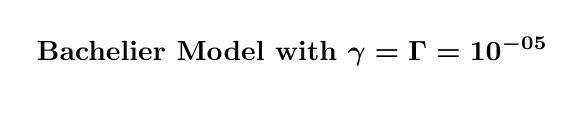
\begin{tikzpicture}[%
font=\footnotesize
]

\begin{axis}[%
width=0.951\figwidth,
height=\figheight,
at={(0\figwidth,0\figheight)},
scale only axis,
xmin=0,
xmax=3,
tick align=outside,
xlabel={$\bar P - p$},
xmajorgrids,
ymin=0,
ymax=1,
ylabel={$T-t$},
ymajorgrids,
zmin=0,
zmax=10000,
zlabel={Relative Increase $\bar u_{\mathrm{BA}} / \bar u_{\mathrm{AC}}$},
zmajorgrids,
view={50}{40},
axis background/.style={fill=white},
title style={font=\bfseries},
title={Bachelier Model with $\boldsymbol{\gamma = \Gamma = 10^{-05}}$},
axis x line*=bottom,
axis y line*=left,
axis z line*=left
]

\addplot3[%
surf,
shader=flat corner,draw=black,z buffer=sort,colormap={mymap}{[1pt] rgb(0pt)=(0.2081,0.1663,0.5292); rgb(1pt)=(0.211624,0.189781,0.577676); rgb(2pt)=(0.212252,0.213771,0.626971); rgb(3pt)=(0.2081,0.2386,0.677086); rgb(4pt)=(0.195905,0.264457,0.7279); rgb(5pt)=(0.170729,0.291938,0.779248); rgb(6pt)=(0.125271,0.324243,0.830271); rgb(7pt)=(0.0591333,0.359833,0.868333); rgb(8pt)=(0.0116952,0.38751,0.881957); rgb(9pt)=(0.00595714,0.408614,0.882843); rgb(10pt)=(0.0165143,0.4266,0.878633); rgb(11pt)=(0.0328524,0.443043,0.871957); rgb(12pt)=(0.0498143,0.458571,0.864057); rgb(13pt)=(0.0629333,0.47369,0.855438); rgb(14pt)=(0.0722667,0.488667,0.8467); rgb(15pt)=(0.0779429,0.503986,0.838371); rgb(16pt)=(0.0793476,0.520024,0.831181); rgb(17pt)=(0.0749429,0.537543,0.826271); rgb(18pt)=(0.0640571,0.556986,0.823957); rgb(19pt)=(0.0487714,0.577224,0.822829); rgb(20pt)=(0.0343429,0.596581,0.819852); rgb(21pt)=(0.0265,0.6137,0.8135); rgb(22pt)=(0.0238905,0.628662,0.803762); rgb(23pt)=(0.0230905,0.641786,0.791267); rgb(24pt)=(0.0227714,0.653486,0.776757); rgb(25pt)=(0.0266619,0.664195,0.760719); rgb(26pt)=(0.0383714,0.674271,0.743552); rgb(27pt)=(0.0589714,0.683757,0.725386); rgb(28pt)=(0.0843,0.692833,0.706167); rgb(29pt)=(0.113295,0.7015,0.685857); rgb(30pt)=(0.145271,0.709757,0.664629); rgb(31pt)=(0.180133,0.717657,0.642433); rgb(32pt)=(0.217829,0.725043,0.619262); rgb(33pt)=(0.258643,0.731714,0.595429); rgb(34pt)=(0.302171,0.737605,0.571186); rgb(35pt)=(0.348167,0.742433,0.547267); rgb(36pt)=(0.395257,0.7459,0.524443); rgb(37pt)=(0.44201,0.748081,0.503314); rgb(38pt)=(0.487124,0.749062,0.483976); rgb(39pt)=(0.530029,0.749114,0.466114); rgb(40pt)=(0.570857,0.748519,0.44939); rgb(41pt)=(0.609852,0.747314,0.433686); rgb(42pt)=(0.6473,0.7456,0.4188); rgb(43pt)=(0.683419,0.743476,0.404433); rgb(44pt)=(0.71841,0.741133,0.390476); rgb(45pt)=(0.752486,0.7384,0.376814); rgb(46pt)=(0.785843,0.735567,0.363271); rgb(47pt)=(0.818505,0.732733,0.34979); rgb(48pt)=(0.850657,0.7299,0.336029); rgb(49pt)=(0.882433,0.727433,0.3217); rgb(50pt)=(0.913933,0.725786,0.306276); rgb(51pt)=(0.944957,0.726114,0.288643); rgb(52pt)=(0.973895,0.731395,0.266648); rgb(53pt)=(0.993771,0.745457,0.240348); rgb(54pt)=(0.999043,0.765314,0.216414); rgb(55pt)=(0.995533,0.786057,0.196652); rgb(56pt)=(0.988,0.8066,0.179367); rgb(57pt)=(0.978857,0.827143,0.163314); rgb(58pt)=(0.9697,0.848138,0.147452); rgb(59pt)=(0.962586,0.870514,0.1309); rgb(60pt)=(0.958871,0.8949,0.113243); rgb(61pt)=(0.959824,0.921833,0.0948381); rgb(62pt)=(0.9661,0.951443,0.0755333); rgb(63pt)=(0.9763,0.9831,0.0538)},mesh/rows=25]
table[row sep=crcr, point meta=\thisrow{c}] {%
%
x	y	z	c\\
0	0.01	1974.96309626365	1974.96309626365\\
0	0.0302040816326531	3365.04198551965	3365.04198551965\\
0	0.0504081632653061	4263.57447993471	4263.57447993471\\
0	0.0706122448979592	4950.96518017001	4950.96518017001\\
0	0.0908163265306122	5510.77858262416	5510.77858262416\\
0	0.111020408163265	5982.22234617453	5982.22234617453\\
0	0.131224489795918	6387.66853314459	6387.66853314459\\
0	0.151428571428571	6741.41676228058	6741.41676228058\\
0	0.171632653061224	7053.31523711875	7053.31523711875\\
0	0.191836734693878	7330.51449582806	7330.51449582806\\
0	0.212040816326531	7578.41451468202	7578.41451468202\\
0	0.232244897959184	7801.2187736762	7801.2187736762\\
0	0.252448979591837	8002.27894312956	8002.27894312956\\
0	0.27265306122449	8184.32004544648	8184.32004544648\\
0	0.292857142857143	8349.59350468048	8349.59350468048\\
0	0.313061224489796	8499.98467031539	8499.98467031539\\
0	0.333265306122449	8637.0904894406	8637.0904894406\\
0	0.353469387755102	8762.27696503074	8762.27696503074\\
0	0.373673469387755	8876.72254265585	8876.72254265585\\
0	0.393877551020408	8981.45146327109	8981.45146327109\\
0	0.414081632653061	9077.35980883525	9077.35980883525\\
0	0.434285714285714	9165.23612648877	9165.23612648877\\
0	0.454489795918367	9245.77796321829	9245.77796321829\\
0	0.47469387755102	9319.60526959909	9319.60526959909\\
0	0.494897959183673	9387.27137432851	9387.27137432851\\
0	0.515102040816326	9449.27205112045	9449.27205112045\\
0	0.53530612244898	9506.05307102769	9506.05307102769\\
0	0.555510204081633	9558.01654024523	9558.01654024523\\
0	0.575714285714286	9605.52625499328	9605.52625499328\\
0	0.595918367346939	9648.91225433548	9648.91225433548\\
0	0.616122448979592	9688.47471328916	9688.47471328916\\
0	0.636326530612245	9724.48728961435	9724.48728961435\\
0	0.656530612244898	9757.20001501668	9757.20001501668\\
0	0.676734693877551	9786.84180424417	9786.84180424417\\
0	0.696938775510204	9813.62264178272	9813.62264178272\\
0	0.717142857142857	9837.73549513092	9837.73549513092\\
0	0.73734693877551	9859.35799502224	9859.35799502224\\
0	0.757551020408163	9878.65391609711	9878.65391609711\\
0	0.777755102040816	9895.77448594058	9895.77448594058\\
0	0.797959183673469	9910.85954593469	9910.85954593469\\
0	0.818163265306122	9924.03858364032	9924.03858364032\\
0	0.838367346938775	9935.43165341904	9935.43165341904\\
0	0.858571428571429	9945.15019950286	9945.15019950286\\
0	0.878775510204082	9953.29779360535	9953.29779360535\\
0	0.898979591836735	9959.97079751215	9959.97079751215\\
0	0.919183673469388	9965.25895951659	9965.25895951659\\
0	0.939387755102041	9969.24595248237	9969.24595248237\\
0	0.959591836734694	9972.00986014532	9972.00986014532\\
0	0.979795918367347	9973.62361750042	9973.62361750042\\
0	1	9974.1554103026	9974.1554103026\\
0.125	0.01	9.92147280337729	9.92147280337729\\
0.125	0.0302040816326531	283.991794756242	283.991794756242\\
0.125	0.0504081632653061	713.988935350244	713.988935350244\\
0.125	0.0706122448979592	1155.87668843731	1155.87668843731\\
0.125	0.0908163265306122	1575.64885183486	1575.64885183486\\
0.125	0.111020408163265	1965.82875141019	1965.82875141019\\
0.125	0.131224489795918	2326.17924377611	2326.17924377611\\
0.125	0.151428571428571	2658.58145313341	2658.58145313341\\
0.125	0.171632653061224	2965.44392825201	2965.44392825201\\
0.125	0.191836734693878	3249.16910148789	3249.16910148789\\
0.125	0.212040816326531	3511.97775242281	3511.97775242281\\
0.125	0.232244897959184	3755.86356159141	3755.86356159141\\
0.125	0.252448979591837	3982.59579989466	3982.59579989466\\
0.125	0.27265306122449	4193.73875474473	4193.73875474473\\
0.125	0.292857142857143	4390.67549273031	4390.67549273031\\
0.125	0.313061224489796	4574.63111691887	4574.63111691887\\
0.125	0.333265306122449	4746.69378859348	4746.69378859348\\
0.125	0.353469387755102	4907.83307522633	4907.83307522633\\
0.125	0.373673469387755	5058.91570735619	5058.91570735619\\
0.125	0.393877551020408	5200.71901539215	5200.71901539215\\
0.125	0.414081632653061	5333.94236310866	5333.94236310866\\
0.125	0.434285714285714	5459.21688172363	5459.21688172363\\
0.125	0.454489795918367	5577.11377434224	5577.11377434224\\
0.125	0.47469387755102	5688.15142158971	5688.15142158971\\
0.125	0.494897959183673	5792.8014835942	5792.8014835942\\
0.125	0.515102040816326	5891.49415280506	5891.49415280506\\
0.125	0.53530612244898	5984.62270472782	5984.62270472782\\
0.125	0.555510204081633	6072.54744345716	6072.54744345716\\
0.125	0.575714285714286	6155.59914085999	6155.59914085999\\
0.125	0.595918367346939	6234.0820434644	6234.0820434644\\
0.125	0.616122448979592	6308.27650813354	6308.27650813354\\
0.125	0.636326530612245	6378.44133585917	6378.44133585917\\
0.125	0.656530612244898	6444.81580122124	6444.81580122124\\
0.125	0.676734693877551	6507.62148307038	6507.62148307038\\
0.125	0.696938775510204	6567.06387305364	6567.06387305364\\
0.125	0.717142857142857	6623.33379794439	6623.33379794439\\
0.125	0.73734693877551	6676.60875348656	6676.60875348656\\
0.125	0.757551020408163	6727.05397921091	6727.05397921091\\
0.125	0.777755102040816	6774.82353264126	6774.82353264126\\
0.125	0.797959183673469	6820.0612046302	6820.0612046302\\
0.125	0.818163265306122	6862.901353435	6862.901353435\\
0.125	0.838367346938775	6903.4696578376	6903.4696578376\\
0.125	0.858571428571429	6941.88379849943	6941.88379849943\\
0.125	0.878775510204082	6978.25407554565	6978.25407554565\\
0.125	0.898979591836735	7012.6839693526	7012.6839693526\\
0.125	0.919183673469388	7045.27065063787	7045.27065063787\\
0.125	0.939387755102041	7076.10544520183	7076.10544520183\\
0.125	0.959591836734694	7105.27425802255	7105.27425802255\\
0.125	0.979795918367347	7132.85796084778	7132.85796084778\\
0.125	1	7158.93274694354	7158.93274694354\\
0.25	0.01	0.000264661675628773	0.000264661675628773\\
0.25	0.0302040816326531	4.94481512403089	4.94481512403089\\
0.25	0.0504081632653061	48.3523472109153	48.3523472109153\\
0.25	0.0706122448979592	143.879074922737	143.879074922737\\
0.25	0.0908163265306122	278.867449055009	278.867449055009\\
0.25	0.111020408163265	438.846094471128	438.846094471128\\
0.25	0.131224489795918	613.098033077107	613.098033077107\\
0.25	0.151428571428571	794.385467524295	794.385467524295\\
0.25	0.171632653061224	977.938077560551	977.938077560551\\
0.25	0.191836734693878	1160.63563277754	1160.63563277754\\
0.25	0.212040816326531	1340.45059975089	1340.45059975089\\
0.25	0.232244897959184	1516.08265781078	1516.08265781078\\
0.25	0.252448979591837	1686.7198471511	1686.7198471511\\
0.25	0.27265306122449	1851.88110276465	1851.88110276465\\
0.25	0.292857142857143	2011.31112041702	2011.31112041702\\
0.25	0.313061224489796	2164.90922137353	2164.90922137353\\
0.25	0.333265306122449	2312.68061206371	2312.68061206371\\
0.25	0.353469387755102	2454.70261253991	2454.70261253991\\
0.25	0.373673469387755	2591.10103370626	2591.10103370626\\
0.25	0.393877551020408	2722.03352774333	2722.03352774333\\
0.25	0.414081632653061	2847.67778849106	2847.67778849106\\
0.25	0.434285714285714	2968.22316206381	2968.22316206381\\
0.25	0.454489795918367	3083.86467852624	3083.86467852624\\
0.25	0.47469387755102	3194.79881670895	3194.79881670895\\
0.25	0.494897959183673	3301.22051839696	3301.22051839696\\
0.25	0.515102040816326	3403.32110823404	3403.32110823404\\
0.25	0.53530612244898	3501.28687298118	3501.28687298118\\
0.25	0.555510204081633	3595.29812207001	3595.29812207001\\
0.25	0.575714285714286	3685.52859982687	3685.52859982687\\
0.25	0.595918367346939	3772.14515440839	3772.14515440839\\
0.25	0.616122448979592	3855.30759351051	3855.30759351051\\
0.25	0.636326530612245	3935.16867511392	3935.16867511392\\
0.25	0.656530612244898	4011.87419486148	4011.87419486148\\
0.25	0.676734693877551	4085.56314149202	4085.56314149202\\
0.25	0.696938775510204	4156.36789904215	4156.36789904215\\
0.25	0.717142857142857	4224.41447995671	4224.41447995671\\
0.25	0.73734693877551	4289.82277731191	4289.82277731191\\
0.25	0.757551020408163	4352.70682740643	4352.70682740643\\
0.25	0.777755102040816	4413.17507627448	4413.17507627448\\
0.25	0.797959183673469	4471.33064540993	4471.33064540993\\
0.25	0.818163265306122	4527.27159330272	4527.27159330272\\
0.25	0.838367346938775	4581.09117038049	4581.09117038049\\
0.25	0.858571428571429	4632.8780656987	4632.8780656987\\
0.25	0.878775510204082	4682.71664428845	4682.71664428845\\
0.25	0.898979591836735	4730.68717449693	4730.68717449693\\
0.25	0.919183673469388	4776.86604497417	4776.86604497417\\
0.25	0.939387755102041	4821.32597119697	4821.32597119697\\
0.25	0.959591836734694	4864.1361915947	4864.1361915947\\
0.25	0.979795918367347	4905.36265346856	4905.36265346856\\
0.25	1	4945.06818898508	4945.06818898508\\
0.375	0.01	2.0372168044195e-11	2.0372168044195e-11\\
0.375	0.0302040816326531	0.0142210136886575	0.0142210136886575\\
0.375	0.0504081632653061	1.16537490505557	1.16537490505557\\
0.375	0.0706122448979592	8.75854730956251	8.75854730956251\\
0.375	0.0908163265306122	28.6654207828827	28.6654207828827\\
0.375	0.111020408163265	63.3299305537992	63.3299305537992\\
0.375	0.131224489795918	112.349043885649	112.349043885649\\
0.375	0.151428571428571	173.939958971314	173.939958971314\\
0.375	0.171632653061224	245.893582416013	245.893582416013\\
0.375	0.191836734693878	326.041694707579	326.041694707579\\
0.375	0.212040816326531	412.446682725297	412.446682725297\\
0.375	0.232244897959184	503.455546554512	503.455546554512\\
0.375	0.252448979591837	597.693652229849	597.693652229849\\
0.375	0.27265306122449	694.035078070687	694.035078070687\\
0.375	0.292857142857143	791.566603878995	791.566603878995\\
0.375	0.313061224489796	889.552737542861	889.552737542861\\
0.375	0.333265306122449	987.404603368754	987.404603368754\\
0.375	0.353469387755102	1084.65342459749	1084.65342459749\\
0.375	0.373673469387755	1180.92843032343	1180.92843032343\\
0.375	0.393877551020408	1275.93867623958	1275.93867623958\\
0.375	0.414081632653061	1369.45818496117	1369.45818496117\\
0.375	0.434285714285714	1461.3138387603	1461.3138387603\\
0.375	0.454489795918367	1551.37552599195	1551.37552599195\\
0.375	0.47469387755102	1639.54812042783	1639.54812042783\\
0.375	0.494897959183673	1725.76494642127	1725.76494642127\\
0.375	0.515102040816326	1809.9824472489	1809.9824472489\\
0.375	0.53530612244898	1892.17582804661	1892.17582804661\\
0.375	0.555510204081633	1972.3354891303	1972.3354891303\\
0.375	0.575714285714286	2050.46410143739	2050.46410143739\\
0.375	0.595918367346939	2126.57420473209	2126.57420473209\\
0.375	0.616122448979592	2200.6862323778	2200.6862323778\\
0.375	0.636326530612245	2272.82688500715	2272.82688500715\\
0.375	0.656530612244898	2343.02779024152	2343.02779024152\\
0.375	0.676734693877551	2411.32439748056	2411.32439748056\\
0.375	0.696938775510204	2477.75506630212	2477.75506630212\\
0.375	0.717142857142857	2542.36031466555	2542.36031466555\\
0.375	0.73734693877551	2605.18219927759	2605.18219927759\\
0.375	0.757551020408163	2666.26380546191	2666.26380546191\\
0.375	0.777755102040816	2725.64882790927	2725.64882790927\\
0.375	0.797959183673469	2783.38122696376	2783.38122696376\\
0.375	0.818163265306122	2839.50494777173	2839.50494777173\\
0.375	0.838367346938775	2894.06369180161	2894.06369180161\\
0.375	0.858571428571429	2947.10073203015	2947.10073203015\\
0.375	0.878775510204082	2998.65876455862	2998.65876455862\\
0.375	0.898979591836735	3048.77979063093	3048.77979063093\\
0.375	0.919183673469388	3097.50502402352	3097.50502402352\\
0.375	0.939387755102041	3144.87481960267	3144.87481960267\\
0.375	0.959591836734694	3190.92861952926	3190.92861952926\\
0.375	0.979795918367347	3235.70491416071	3235.70491416071\\
0.375	1	3279.24121517363	3279.24121517363\\
0.5	0.01	3.70027740467147e-21	3.70027740467147e-21\\
0.5	0.0302040816326531	6.05166275757194e-06	6.05166275757194e-06\\
0.5	0.0504081632653061	0.00928362193282868	0.00928362193282868\\
0.5	0.0706122448979592	0.246863462130324	0.246863462130324\\
0.5	0.0908163265306122	1.63961009409722	1.63961009409722\\
0.5	0.111020408163265	5.7056963654387	5.7056963654387\\
0.5	0.131224489795918	13.9032467007824	13.9032467007824\\
0.5	0.151428571428571	27.22458772747	27.22458772747\\
0.5	0.171632653061224	46.1353141864234	46.1353141864234\\
0.5	0.191836734693878	70.6760227745324	70.6760227745324\\
0.5	0.212040816326531	100.597323523654	100.597323523654\\
0.5	0.232244897959184	135.475914228187	135.475914228187\\
0.5	0.252448979591837	174.799755790083	174.799755790083\\
0.5	0.27265306122449	218.025385259969	218.025385259969\\
0.5	0.292857142857143	264.614085705389	264.614085705389\\
0.5	0.313061224489796	314.053260487906	314.053260487906\\
0.5	0.333265306122449	365.867939460128	365.867939460128\\
0.5	0.353469387755102	419.625933320643	419.625933320643\\
0.5	0.373673469387755	474.939035340199	474.939035340199\\
0.5	0.393877551020408	531.461862545532	531.461862545532\\
0.5	0.414081632653061	588.889371301841	588.889371301841\\
0.5	0.434285714285714	646.95370748814	646.95370748814\\
0.5	0.454489795918367	705.420803499627	705.420803499627\\
0.5	0.47469387755102	764.086972201466	764.086972201466\\
0.5	0.494897959183673	822.775643102769	822.775643102769\\
0.5	0.515102040816326	881.334318985718	881.334318985718\\
0.5	0.53530612244898	939.631789008083	939.631789008083\\
0.5	0.555510204081633	997.555608270507	997.555608270507\\
0.5	0.575714285714286	1055.00983830871	1055.00983830871\\
0.5	0.595918367346939	1111.91303418956	1111.91303418956\\
0.5	0.616122448979592	1168.19645940182	1168.19645940182\\
0.5	0.636326530612245	1223.80250792952	1223.80250792952\\
0.5	0.656530612244898	1278.68331273193	1278.68331273193\\
0.5	0.676734693877551	1332.79952065	1332.79952065\\
0.5	0.696938775510204	1386.11921507993	1386.11921507993\\
0.5	0.717142857142857	1438.61696932374	1438.61696932374\\
0.5	0.73734693877551	1490.2730151732	1490.2730151732\\
0.5	0.757551020408163	1541.07251290356	1541.07251290356\\
0.5	0.777755102040816	1591.00491038821	1591.00491038821\\
0.5	0.797959183673469	1640.06338046379	1640.06338046379\\
0.5	0.818163265306122	1688.24432696453	1688.24432696453\\
0.5	0.838367346938775	1735.54695100258	1735.54695100258\\
0.5	0.858571428571429	1781.97287010269	1781.97287010269\\
0.5	0.878775510204082	1827.52578371256	1827.52578371256\\
0.5	0.898979591836735	1872.21117941497	1872.21117941497\\
0.5	0.919183673469388	1916.03607487464	1916.03607487464\\
0.5	0.939387755102041	1959.0087911722	1959.0087911722\\
0.5	0.959591836734694	2001.13875371946	2001.13875371946\\
0.5	0.979795918367347	2042.43631742397	2042.43631742397\\
0.5	1	2082.91261318422	2082.91261318422\\
0.625	0.01	1.4599002273823e-33	1.4599002273823e-33\\
0.625	0.0302040816326531	3.59943162273761e-10	3.59943162273761e-10\\
0.625	0.0504081632653061	2.34139909973678e-05	2.34139909973678e-05\\
0.625	0.0706122448979592	0.00311297318849802	0.00311297318849802\\
0.625	0.0908163265306122	0.050728572443546	0.050728572443546\\
0.625	0.111020408163265	0.313335687202265	0.313335687202265\\
0.625	0.131224489795918	1.13815087523636	1.13815087523636\\
0.625	0.151428571428571	2.99132617723036	2.99132617723036\\
0.625	0.171632653061224	6.35640104420783	6.35640104420783\\
0.625	0.191836734693878	11.6537159975422	11.6537159975422\\
0.625	0.212040816326531	19.1992849376957	19.1992849376957\\
0.625	0.232244897959184	29.1954520758597	29.1954520758597\\
0.625	0.252448979591837	41.7402010979759	41.7402010979759\\
0.625	0.27265306122449	56.8447357410156	56.8447357410156\\
0.625	0.292857142857143	74.4529740299902	74.4529740299902\\
0.625	0.313061224489796	94.4596873535218	94.4596873535218\\
0.625	0.333265306122449	116.725933949513	116.725933949513\\
0.625	0.353469387755102	141.091483499217	141.091483499217\\
0.625	0.373673469387755	167.384434268943	167.384434268943\\
0.625	0.393877551020408	195.428424209579	195.428424209579\\
0.625	0.414081632653061	225.04788011539	225.04788011539\\
0.625	0.434285714285714	256.071718485635	256.071718485635\\
0.625	0.454489795918367	288.335853141625	288.335853141625\\
0.625	0.47469387755102	321.684800459271	321.684800459271\\
0.625	0.494897959183673	355.972613528885	355.972613528885\\
0.625	0.515102040816326	391.063325493969	391.063325493969\\
0.625	0.53530612244898	426.831040446985	426.831040446985\\
0.625	0.555510204081633	463.159776862868	463.159776862868\\
0.625	0.575714285714286	499.943142404706	499.943142404706\\
0.625	0.595918367346939	537.083898731954	537.083898731954\\
0.625	0.616122448979592	574.493459479506	574.493459479506\\
0.625	0.636326530612245	612.091352832482	612.091352832482\\
0.625	0.656530612244898	649.804671259241	649.804671259241\\
0.625	0.676734693877551	687.56752431613	687.56752431613\\
0.625	0.696938775510204	725.320505478096	725.320505478096\\
0.625	0.717142857142857	763.010180273523	763.010180273523\\
0.625	0.73734693877551	800.588600297086	800.588600297086\\
0.625	0.757551020408163	838.012845702134	838.012845702134\\
0.625	0.777755102040816	875.244597352097	875.244597352097\\
0.625	0.797959183673469	912.249738800325	912.249738800325\\
0.625	0.818163265306122	948.997987564943	948.997987564943\\
0.625	0.838367346938775	985.462554690382	985.462554690382\\
0.625	0.858571428571429	1021.61983128059	1021.61983128059\\
0.625	0.878775510204082	1057.44910050535	1057.44910050535\\
0.625	0.898979591836735	1092.93227348679	1092.93227348679\\
0.625	0.919183673469388	1128.05364744299	1128.05364744299\\
0.625	0.939387755102041	1162.79968447985	1162.79968447985\\
0.625	0.959591836734694	1197.158809468	1197.158809468\\
0.625	0.979795918367347	1231.12122550712	1231.12122550712\\
0.625	1	1264.67874555857	1264.67874555857\\
0.75	0.01	1.20100252297147e-48	1.20100252297147e-48\\
0.75	0.0302040816326531	2.89826150829227e-15	2.89826150829227e-15\\
0.75	0.0504081632653061	1.82140035560565e-08	1.82140035560565e-08\\
0.75	0.0706122448979592	1.71808743416325e-05	1.71808743416325e-05\\
0.75	0.0908163265306122	0.000833078017839609	0.000833078017839609\\
0.75	0.111020408163265	0.0103165496102228	0.0103165496102228\\
0.75	0.131224489795918	0.0607381402524389	0.0607381402524389\\
0.75	0.151428571428571	0.227726878881842	0.227726878881842\\
0.75	0.171632653061224	0.635535516454963	0.635535516454963\\
0.75	0.191836734693878	1.44601579266	1.44601579266\\
0.75	0.212040816326531	2.83910447247449	2.83910447247449\\
0.75	0.232244897959184	4.99318791399164	4.99318791399164\\
0.75	0.252448979591837	8.06997956411563	8.06997956411563\\
0.75	0.27265306122449	12.2051258538164	12.2051258538164\\
0.75	0.292857142857143	17.5038773514122	17.5038773514122\\
0.75	0.313061224489796	24.0405043870059	24.0405043870059\\
0.75	0.333265306122449	31.860135298583	31.860135298583\\
0.75	0.353469387755102	40.98195176406	40.98195176406\\
0.75	0.373673469387755	51.4029793527869	51.4029793527869\\
0.75	0.393877551020408	63.1019752114528	63.1019752114528\\
0.75	0.414081632653061	76.0431148325365	76.0431148325365\\
0.75	0.434285714285714	90.1793195257052	90.1793195257052\\
0.75	0.454489795918367	105.455157790248	105.455157790248\\
0.75	0.47469387755102	121.809310340721	121.809310340721\\
0.75	0.494897959183673	139.176621038661	139.176621038661\\
0.75	0.515102040816326	157.489772702193	157.489772702193\\
0.75	0.53530612244898	176.680633562674	176.680633562674\\
0.75	0.555510204081633	196.681320991351	196.681320991351\\
0.75	0.575714285714286	217.425026639423	217.425026639423\\
0.75	0.595918367346939	238.846642981545	238.846642981545\\
0.75	0.616122448979592	260.883226445084	260.883226445084\\
0.75	0.636326530612245	283.474327445059	283.474327445059\\
0.75	0.656530612244898	306.562213058212	306.562213058212\\
0.75	0.676734693877551	330.092003921597	330.092003921597\\
0.75	0.696938775510204	354.011743292166	354.011743292166\\
0.75	0.717142857142857	378.272413055788	378.272413055788\\
0.75	0.73734693877551	402.827908796289	402.827908796289\\
0.75	0.757551020408163	427.634983781476	427.634983781476\\
0.75	0.777755102040816	452.653169842289	452.653169842289\\
0.75	0.797959183673469	477.844681561764	477.844681561764\\
0.75	0.818163265306122	503.174308904711	503.174308904711\\
0.75	0.838367346938775	528.609302363718	528.609302363718\\
0.75	0.858571428571429	554.119253834547	554.119253834547\\
0.75	0.878775510204082	579.675975731653	579.675975731653\\
0.75	0.898979591836735	605.253380284764	605.253380284764\\
0.75	0.919183673469388	630.827360496802	630.827360496802\\
0.75	0.939387755102041	656.375673872534	656.375673872534\\
0.75	0.959591836734694	681.877829729784	681.877829729784\\
0.75	0.979795918367347	707.314980667563	707.314980667563\\
0.75	1	732.669818576851	732.669818576851\\
0.875	0.01	2.01341524397776e-66	2.01341524397776e-66\\
0.875	0.0302040816326531	3.09891861655145e-21	3.09891861655145e-21\\
0.875	0.0504081632653061	4.29830087735051e-12	4.29830087735051e-12\\
0.875	0.0706122448979592	4.09024928351304e-08	4.09024928351304e-08\\
0.875	0.0908163265306122	7.16854966049306e-06	7.16854966049306e-06\\
0.875	0.111020408163265	0.000201302550273641	0.000201302550273641\\
0.875	0.131224489795918	0.00209095277372405	0.00209095277372405\\
0.875	0.151428571428571	0.0118975225116383	0.0118975225116383\\
0.875	0.171632653061224	0.0457092645049521	0.0457092645049521\\
0.875	0.191836734693878	0.133929863884871	0.133929863884871\\
0.875	0.212040816326531	0.322857658228276	0.322857658228276\\
0.875	0.232244897959184	0.672993360836977	0.672993360836977\\
0.875	0.252448979591837	1.25502942995517	1.25502942995517\\
0.875	0.27265306122449	2.14486243391176	2.14486243391176\\
0.875	0.292857142857143	3.41872649908407	3.41872649908407\\
0.875	0.313061224489796	5.14910628078819	5.14910628078819\\
0.875	0.333265306122449	7.4016983966252	7.4016983966252\\
0.875	0.353469387755102	10.2334288418834	10.2334288418834\\
0.875	0.373673469387755	13.6913928715741	13.6913928715741\\
0.875	0.393877551020408	17.8125284322855	17.8125284322855\\
0.875	0.414081632653061	22.6238300778229	22.6238300778229\\
0.875	0.434285714285714	28.1429320232219	28.1429320232219\\
0.875	0.454489795918367	34.3789205407307	34.3789205407307\\
0.875	0.47469387755102	41.3332683222907	41.3332683222907\\
0.875	0.494897959183673	49.0008124004057	49.0008124004057\\
0.875	0.515102040816326	57.3707211367665	57.3707211367665\\
0.875	0.53530612244898	66.4274145164274	66.4274145164274\\
0.875	0.555510204081633	76.1514160675396	76.1514160675396\\
0.875	0.575714285714286	86.5201249504835	86.5201249504835\\
0.875	0.595918367346939	97.5085039322378	97.5085039322378\\
0.875	0.616122448979592	109.08968380379	109.08968380379\\
0.875	0.636326530612245	121.235487911221	121.235487911221\\
0.875	0.656530612244898	133.916882332679	133.916882332679\\
0.875	0.676734693877551	147.104358211765	147.104358211765\\
0.875	0.696938775510204	160.768253129468	160.768253129468\\
0.875	0.717142857142857	174.879018365126	174.879018365126\\
0.875	0.73734693877551	189.407438609066	189.407438609066\\
0.875	0.757551020408163	204.324810249841	204.324810249841\\
0.875	0.777755102040816	219.603083839825	219.603083839825\\
0.875	0.797959183673469	235.214975793533	235.214975793533\\
0.875	0.818163265306122	251.13405382589	251.13405382589\\
0.875	0.838367346938775	267.33480011309	267.33480011309\\
0.875	0.858571428571429	283.792655668825	283.792655668825\\
0.875	0.878775510204082	300.484048979709	300.484048979709\\
0.875	0.898979591836735	317.386411538087	317.386411538087\\
0.875	0.919183673469388	334.478182547899	334.478182547899\\
0.875	0.939387755102041	351.738804758043	351.738804758043\\
0.875	0.959591836734694	369.148713095132	369.148713095132\\
0.875	0.979795918367347	386.689317520314	386.689317520314\\
0.875	1	404.342981319644	404.342981319644\\
1	0.01	6.78224007256495e-87	6.78224007256495e-87\\
1	0.0302040816326531	4.34578041141234e-28	4.34578041141234e-28\\
1	0.0504081632653061	3.04331917211728e-16	3.04331917211728e-16\\
1	0.0706122448979592	4.15872448463928e-11	4.15872448463928e-11\\
1	0.0908163265306122	3.20297664721072e-08	3.20297664721072e-08\\
1	0.111020408163265	2.30860834384424e-06	2.30860834384424e-06\\
1	0.131224489795918	4.6081622886484e-05	4.6081622886484e-05\\
1	0.151428571428571	0.000423560722234804	0.000423560722234804\\
1	0.171632653061224	0.00234933032536848	0.00234933032536848\\
1	0.191836734693878	0.00920250347578399	0.00920250347578399\\
1	0.212040816326531	0.0280717897660808	0.0280717897660808\\
1	0.232244897959184	0.0710983085899604	0.0710983085899604\\
1	0.252448979591837	0.156199172935421	0.156199172935421\\
1	0.27265306122449	0.307017264627121	0.307017264627121\\
1	0.292857142857143	0.552183325030938	0.552183325030938\\
1	0.313061224489796	0.924107336290017	0.924107336290017\\
1	0.333265306122449	1.45754264537834	1.45754264537834\\
1	0.353469387755102	2.18812935599859	2.18812935599859\\
1	0.373673469387755	3.15106216275091	3.15106216275091\\
1	0.393877551020408	4.37996680081405	4.37996680081405\\
1	0.414081632653061	5.90602012494154	5.90602012494154\\
1	0.434285714285714	7.75731440631033	7.75731440631033\\
1	0.454489795918367	9.95844528971591	9.95844528971591\\
1	0.47469387755102	12.5302919547281	12.5302919547281\\
1	0.494897959183673	15.4899542313105	15.4899542313105\\
1	0.515102040816326	18.8508121023049	18.8508121023049\\
1	0.53530612244898	22.6226762200985	22.6226762200985\\
1	0.555510204081633	26.8120024257073	26.8120024257073\\
1	0.575714285714286	31.4221479263837	31.4221479263837\\
1	0.595918367346939	36.4536512580835	36.4536512580835\\
1	0.616122448979592	41.9045221683777	41.9045221683777\\
1	0.636326530612245	47.7705309952826	47.7705309952826\\
1	0.656530612244898	54.0454899731345	54.0454899731345\\
1	0.676734693877551	60.7215212051757	60.7215212051757\\
1	0.696938775510204	67.7893078662823	67.7893078662823\\
1	0.717142857142857	75.2383266093548	75.2383266093548\\
1	0.73734693877551	83.0570602156456	83.0570602156456\\
1	0.757551020408163	91.2331903172953	91.2331903172953\\
1	0.777755102040816	99.7537705861359	99.7537705861359\\
1	0.797959183673469	108.605381174376	108.605381174376\\
1	0.818163265306122	117.774265449846	117.774265449846\\
1	0.838367346938775	127.246450223359	127.246450223359\\
1	0.858571428571429	137.007850744291	137.007850744291\\
1	0.878775510204082	147.044361763157	147.044361763157\\
1	0.898979591836735	157.341935942717	157.341935942717\\
1	0.919183673469388	167.886650854245	167.886650854245\\
1	0.939387755102041	178.664765732531	178.664765732531\\
1	0.959591836734694	189.662769088864	189.662769088864\\
1	0.979795918367347	200.867418201085	200.867418201085\\
1	1	212.265771417455	212.265771417455\\
1.125	0.01	4.54827690144544e-110	4.54827690144544e-110\\
1.125	0.0302040816326531	7.9262569408573e-36	7.9262569408573e-36\\
1.125	0.0504081632653061	6.41545694515423e-21	6.41545694515423e-21\\
1.125	0.0706122448979592	1.79312907691281e-14	1.79312907691281e-14\\
1.125	0.0908163265306122	7.38271721658711e-11	7.38271721658711e-11\\
1.125	0.111020408163265	1.54667403963629e-08	1.54667403963629e-08\\
1.125	0.131224489795918	6.46468700125689e-07	6.46468700125689e-07\\
1.125	0.151428571428571	1.02207110157489e-05	1.02207110157489e-05\\
1.125	0.171632653061224	8.5859033920484e-05	8.5859033920484e-05\\
1.125	0.191836734693878	0.000466883373538433	0.000466883373538433\\
1.125	0.212040816326531	0.00185788598374998	0.00185788598374998\\
1.125	0.232244897959184	0.00586252339354583	0.00586252339354583\\
1.125	0.252448979591837	0.0154952873225952	0.0154952873225952\\
1.125	0.27265306122449	0.0356589633474257	0.0356589633474257\\
1.125	0.292857142857143	0.0734859245705103	0.0734859245705103\\
1.125	0.313061224489796	0.138483806279551	0.138483806279551\\
1.125	0.333265306122449	0.242474571136689	0.242474571136689\\
1.125	0.353469387755102	0.399353397896566	0.399353397896566\\
1.125	0.373673469387755	0.624714569481915	0.624714569481915\\
1.125	0.393877551020408	0.935397440091968	0.935397440091968\\
1.125	0.414081632653061	1.34900139488532	1.34900139488532\\
1.125	0.434285714285714	1.88340928507584	1.88340928507584\\
1.125	0.454489795918367	2.55634774670056	2.55634774670056\\
1.125	0.47469387755102	3.38500233374214	3.38500233374214\\
1.125	0.494897959183673	4.38569663254051	4.38569663254051\\
1.125	0.515102040816326	5.57363783157702	5.57363783157702\\
1.125	0.53530612244898	6.96272651516738	6.96272651516738\\
1.125	0.555510204081633	8.56542543621694	8.56542543621694\\
1.125	0.575714285714286	10.3926803392264	10.3926803392264\\
1.125	0.595918367346939	12.4538851995051	12.4538851995051\\
1.125	0.616122448979592	14.7568842165604	14.7568842165604\\
1.125	0.636326530612245	17.3080033083158	17.3080033083158\\
1.125	0.656530612244898	20.1121045166599	20.1121045166599\\
1.125	0.676734693877551	23.1726575233837	23.1726575233837\\
1.125	0.696938775510204	26.4918232994602	26.4918232994602\\
1.125	0.717142857142857	30.0705457119509	30.0705457119509\\
1.125	0.73734693877551	33.9086476568068	33.9086476568068\\
1.125	0.757551020408163	38.0049289540238	38.0049289540238\\
1.125	0.777755102040816	42.3572638267122	42.3572638267122\\
1.125	0.797959183673469	46.962696287604	46.962696287604\\
1.125	0.818163265306122	51.8175321797172	51.8175321797172\\
1.125	0.838367346938775	56.9174269692061	56.9174269692061\\
1.125	0.858571428571429	62.2574686758372	62.2574686758372\\
1.125	0.878775510204082	67.8322555583279	67.8322555583279\\
1.125	0.898979591836735	73.6359683559724	73.6359683559724\\
1.125	0.919183673469388	79.6624370319679	79.6624370319679\\
1.125	0.939387755102041	85.9052020743329	85.9052020743329\\
1.125	0.959591836734694	92.3575704931471	92.3575704931471\\
1.125	0.979795918367347	99.0126667131296	99.0126667131296\\
1.125	1	105.863478602655	105.863478602655\\
1.25	0.01	6.03364873317988e-136	6.03364873317988e-136\\
1.25	0.0302040816326531	1.86914310267116e-44	1.86914310267116e-44\\
1.25	0.0504081632653061	4.0044844546327e-26	4.0044844546327e-26\\
1.25	0.0706122448979592	3.26189170127401e-18	3.26189170127401e-18\\
1.25	0.0908163265306122	8.73618955976679e-14	8.73618955976679e-14\\
1.25	0.111020408163265	6.02588614208119e-11	6.02588614208119e-11\\
1.25	0.131224489795918	5.74829967773616e-09	5.74829967773616e-09\\
1.25	0.151428571428571	1.66489892868874e-07	1.66489892868874e-07\\
1.25	0.171632653061224	2.22256671040042e-06	2.22256671040042e-06\\
1.25	0.191836734693878	1.74257406423672e-05	1.74257406423672e-05\\
1.25	0.212040816326531	9.32694119283362e-05	9.32694119283362e-05\\
1.25	0.232244897959184	0.000376042196260204	0.000376042196260204\\
1.25	0.252448979591837	0.00122132036187398	0.00122132036187398\\
1.25	0.27265306122449	0.00335033696262565	0.00335033696262565\\
1.25	0.292857142857143	0.00803437904972179	0.00803437904972179\\
1.25	0.313061224489796	0.0172797361813618	0.0172797361813618\\
1.25	0.333265306122449	0.0339850921332754	0.0339850921332754\\
1.25	0.353469387755102	0.0620497826667037	0.0620497826667037\\
1.25	0.373673469387755	0.106421252007345	0.106421252007345\\
1.25	0.393877551020408	0.17307990693925	0.17307990693925\\
1.25	0.414081632653061	0.268967313923457	0.268967313923457\\
1.25	0.434285714285714	0.401868570450039	0.401868570450039\\
1.25	0.454489795918367	0.580261870479244	0.580261870479244\\
1.25	0.47469387755102	0.813148380989908	0.813148380989908\\
1.25	0.494897959183673	1.10987426580455	1.10987426580455\\
1.25	0.515102040816326	1.47995466904405	1.47995466904405\\
1.25	0.53530612244898	1.9329071861016	1.9329071861016\\
1.25	0.555510204081633	2.47810012727732	2.47810012727732\\
1.25	0.575714285714286	3.12461890531239	3.12461890531239\\
1.25	0.595918367346939	3.88115223958416	3.88115223958416\\
1.25	0.616122448979592	4.7558985857949	4.7558985857949\\
1.25	0.636326530612245	5.75649224907463	5.75649224907463\\
1.25	0.656530612244898	6.88994797788465	6.88994797788465\\
1.25	0.676734693877551	8.1626224153139	8.1626224153139\\
1.25	0.696938775510204	9.58019055274217	9.58019055274217\\
1.25	0.717142857142857	11.147635242373	11.147635242373\\
1.25	0.73734693877551	12.8692478403663	12.8692478403663\\
1.25	0.757551020408163	14.748638138889	14.748638138889\\
1.25	0.777755102040816	16.7887518778033	16.7887518778033\\
1.25	0.797959183673469	18.9918942853786	18.9918942853786\\
1.25	0.818163265306122	21.3597582678874	21.3597582678874\\
1.25	0.838367346938775	23.8934560398931	23.8934560398931\\
1.25	0.858571428571429	26.5935531533724	26.5935531533724\\
1.25	0.878775510204082	29.4601040399874	29.4601040399874\\
1.25	0.898979591836735	32.4926883241283	32.4926883241283\\
1.25	0.919183673469388	35.690447293476	35.690447293476\\
1.25	0.939387755102041	39.0521200284403	39.0521200284403\\
1.25	0.959591836734694	42.5760787922242	42.5760787922242\\
1.25	0.979795918367347	46.2603633702066	46.2603633702066\\
1.25	1	50.1027141218193	50.1027141218193\\
1.375	0.01	1.57607696564515e-164	1.57607696564515e-164\\
1.375	0.0302040816326531	5.67435200522575e-54	5.67435200522575e-54\\
1.375	0.0504081632653061	7.37117847661554e-32	7.37117847661554e-32\\
1.375	0.0706122448979592	2.49380467636285e-22	2.49380467636285e-22\\
1.375	0.0908163265306122	5.28793451126326e-17	5.28793451126326e-17\\
1.375	0.111020408163265	1.36053564644588e-13	1.36053564644588e-13\\
1.375	0.131224489795918	3.22900119512589e-11	3.22900119512589e-11\\
1.375	0.151428571428571	1.82501357433847e-09	1.82501357433847e-09\\
1.375	0.171632653061224	4.06294259873067e-08	4.06294259873067e-08\\
1.375	0.191836734693878	4.7708969954007e-07	4.7708969954007e-07\\
1.375	0.212040816326531	3.5418272460135e-06	3.5418272460135e-06\\
1.375	0.232244897959184	1.87136912041365e-05	1.87136912041365e-05\\
1.375	0.252448979591837	7.62881349978717e-05	7.62881349978717e-05\\
1.375	0.27265306122449	0.000254010502600179	0.000254010502600179\\
1.375	0.292857142857143	0.000719939133498342	0.000719939133498342\\
1.375	0.313061224489796	0.00179118661009446	0.00179118661009446\\
1.375	0.333265306122449	0.00400429362069461	0.00400429362069461\\
1.375	0.353469387755102	0.00819013997348979	0.00819013997348979\\
1.375	0.373673469387755	0.0155452174084068	0.0155452174084068\\
1.375	0.393877551020408	0.0276917337257678	0.0276917337257678\\
1.375	0.414081632653061	0.0467208620473268	0.0467208620473268\\
1.375	0.434285714285714	0.0752158334807532	0.0752158334807532\\
1.375	0.454489795918367	0.116253936986118	0.116253936986118\\
1.375	0.47469387755102	0.173388474044909	0.173388474044909\\
1.375	0.494897959183673	0.250613150197434	0.250613150197434\\
1.375	0.515102040816326	0.352312250656068	0.352312250656068\\
1.375	0.53530612244898	0.483200313085031	0.483200313085031\\
1.375	0.555510204081633	0.648254988645984	0.648254988645984\\
1.375	0.575714285714286	0.852646491468586	0.852646491468586\\
1.375	0.595918367346939	1.10166658369342	1.10166658369342\\
1.375	0.616122448979592	1.40065951412961	1.40065951412961\\
1.375	0.636326530612245	1.75495678657113	1.75495678657113\\
1.375	0.656530612244898	2.1698171213503	2.1698171213503\\
1.375	0.676734693877551	2.65037251615464	2.65037251615464\\
1.375	0.696938775510204	3.20158092194742	3.20158092194742\\
1.375	0.717142857142857	3.82818573032963	3.82818573032963\\
1.375	0.73734693877551	4.53468201718877	4.53468201718877\\
1.375	0.757551020408163	5.32528929776858	5.32528929776858\\
1.375	0.777755102040816	6.20393041234661	6.20393041234661\\
1.375	0.797959183673469	7.17421607093861	7.17421607093861\\
1.375	0.818163265306122	8.23943453148818	8.23943453148818\\
1.375	0.838367346938775	9.40254586115304	9.40254586115304\\
1.375	0.858571428571429	10.6661802277857	10.6661802277857\\
1.375	0.878775510204082	12.0326396827395	12.0326396827395\\
1.375	0.898979591836735	13.5039029219122	13.5039029219122\\
1.375	0.919183673469388	15.0816325455679	15.0816325455679\\
1.375	0.939387755102041	16.7671843758806	16.7671843758806\\
1.375	0.959591836734694	18.5616184319216	18.5616184319216\\
1.375	0.979795918367347	20.4657112031763	20.4657112031763\\
1.375	1	22.4799689032959	22.4799689032959\\
1.5	0.01	8.07899371080351e-196	8.07899371080351e-196\\
1.5	0.0302040816326531	2.21045434375851e-64	2.21045434375851e-64\\
1.5	0.0504081632653061	3.98894453682123e-38	3.98894453682123e-38\\
1.5	0.0706122448979592	7.98934212132805e-27	7.98934212132805e-27\\
1.5	0.0908163265306122	1.63262050113838e-20	1.63262050113838e-20\\
1.5	0.111020408163265	1.77539274584666e-16	1.77539274584666e-16\\
1.5	0.131224489795918	1.14290534003137e-13	1.14290534003137e-13\\
1.5	0.151428571428571	1.34287726272131e-11	1.34287726272131e-11\\
1.5	0.171632653061224	5.23245169984706e-10	5.23245169984706e-10\\
1.5	0.191836734693878	9.55948761020878e-09	9.55948761020878e-09\\
1.5	0.212040816326531	1.01512376695164e-07	1.01512376695164e-07\\
1.5	0.232244897959184	7.20978266061015e-07	7.20978266061015e-07\\
1.5	0.252448979591837	3.76861810158749e-06	3.76861810158749e-06\\
1.5	0.27265306122449	1.55091510251825e-05	1.55091510251825e-05\\
1.5	0.292857142857143	5.27706021849132e-05	5.27706021849132e-05\\
1.5	0.313061224489796	0.000153955012116379	0.000153955012116379\\
1.5	0.333265306122449	0.000395901340185908	0.000395901340185908\\
1.5	0.353469387755102	0.000916731879383617	0.000916731879383617\\
1.5	0.373673469387755	0.00194375212262461	0.00194375212262461\\
1.5	0.393877551020408	0.00382456131794305	0.00382456131794305\\
1.5	0.414081632653061	0.00705897064912495	0.00705897064912495\\
1.5	0.434285714285714	0.0123291847754672	0.0123291847754672\\
1.5	0.454489795918367	0.0205259330189403	0.0205259330189403\\
1.5	0.47469387755102	0.0327687271431753	0.0327687271431753\\
1.5	0.494897959183673	0.050419045182715	0.050419045182715\\
1.5	0.515102040816326	0.0750858826598213	0.0750858826598213\\
1.5	0.53530612244898	0.108623692377154	0.108623692377154\\
1.5	0.555510204081633	0.153123204026137	0.153123204026137\\
1.5	0.575714285714286	0.210895956071894	0.210895956071894\\
1.5	0.595918367346939	0.284453586650787	0.284453586650787\\
1.5	0.616122448979592	0.376483032430792	0.376483032430792\\
1.5	0.636326530612245	0.489818795856078	0.489818795856078\\
1.5	0.656530612244898	0.627413384917817	0.627413384917817\\
1.5	0.676734693877551	0.792306927192642	0.792306927192642\\
1.5	0.696938775510204	0.987596829981362	0.987596829981362\\
1.5	0.717142857142857	1.21640821590411	1.21640821590411\\
1.5	0.73734693877551	1.48186571951971	1.48186571951971\\
1.5	0.757551020408163	1.78706709336509	1.78706709336509\\
1.5	0.777755102040816	2.1350589463857	2.1350589463857\\
1.5	0.797959183673469	2.52881482695828	2.52881482695828\\
1.5	0.818163265306122	2.97121576782345	2.97121576782345\\
1.5	0.838367346938775	3.46503333127577	3.46503333127577\\
1.5	0.858571428571429	4.01291512912037	4.01291512912037\\
1.5	0.878775510204082	4.61737274191315	4.61737274191315\\
1.5	0.898979591836735	5.28077192430217	5.28077192430217\\
1.5	0.919183673469388	6.00532495622367	6.00532495622367\\
1.5	0.939387755102041	6.79308498163688	6.79308498163688\\
1.5	0.959591836734694	7.64594216585572	7.64594216585572\\
1.5	0.979795918367347	8.56562149793549	8.56562149793549\\
1.5	1	9.55368206474199	9.55368206474199\\
1.625	0.01	8.10567676142103e-230	8.10567676142103e-230\\
1.625	0.0302040816326531	1.10218782512953e-75	1.10218782512953e-75\\
1.625	0.0504081632653061	6.33097865958506e-45	6.33097865958506e-45\\
1.625	0.0706122448979592	1.07008142077437e-31	1.07008142077437e-31\\
1.625	0.0908163265306122	2.56542137296568e-24	2.56542137296568e-24\\
1.625	0.111020408163265	1.3361295998413e-19	1.3361295998413e-19\\
1.625	0.131224489795918	2.54373776664276e-16	2.54373776664276e-16\\
1.625	0.151428571428571	6.61966260959137e-14	6.61966260959137e-14\\
1.625	0.171632653061224	4.73821093430765e-12	4.73821093430765e-12\\
1.625	0.191836734693878	1.39922593404562e-10	1.39922593404562e-10\\
1.625	0.212040816326531	2.19195846274572e-09	2.19195846274572e-09\\
1.625	0.232244897959184	2.14667768277707e-08	2.14667768277707e-08\\
1.625	0.252448979591837	1.46983875247098e-07	1.46983875247098e-07\\
1.625	0.27265306122449	7.61348702196558e-07	7.61348702196558e-07\\
1.625	0.292857142857143	3.15898414338228e-06	3.15898414338228e-06\\
1.625	0.313061224489796	1.09552336427476e-05	1.09552336427476e-05\\
1.625	0.333265306122449	3.27955885658864e-05	3.27955885658864e-05\\
1.625	0.353469387755102	8.68869361058914e-05	8.68869361058914e-05\\
1.625	0.373673469387755	0.000207748716979869	0.000207748716979869\\
1.625	0.393877551020408	0.00045533877347892	0.00045533877347892\\
1.625	0.414081632653061	0.000926402472282536	0.000926402472282536\\
1.625	0.434285714285714	0.00176759323745956	0.00176759323745956\\
1.625	0.454489795918367	0.00318967588399273	0.00318967588399273\\
1.625	0.47469387755102	0.00548198510809716	0.00548198510809716\\
1.625	0.494897959183673	0.00902627837023729	0.00902627837023729\\
1.625	0.515102040816326	0.0143091831338845	0.0143091831338845\\
1.625	0.53530612244898	0.0219325690325205	0.0219325690325205\\
1.625	0.555510204081633	0.0326213480564378	0.0326213480564378\\
1.625	0.575714285714286	0.0472283940711534	0.0472283940711534\\
1.625	0.595918367346939	0.0667364557676456	0.0667364557676456\\
1.625	0.616122448979592	0.0922570996802071	0.0922570996802071\\
1.625	0.636326530612245	0.125026853494093	0.125026853494093\\
1.625	0.656530612244898	0.166400820948131	0.166400820948131\\
1.625	0.676734693877551	0.217844108513906	0.217844108513906\\
1.625	0.696938775510204	0.280921443567138	0.280921443567138\\
1.625	0.717142857142857	0.357285378285861	0.357285378285861\\
1.625	0.73734693877551	0.448663467947588	0.448663467947588\\
1.625	0.757551020408163	0.556844791587183	0.556844791587183\\
1.625	0.777755102040816	0.683666151663264	0.683666151663264\\
1.625	0.797959183673469	0.830998251404981	0.830998251404981\\
1.625	0.818163265306122	1.00073210712298	1.00073210712298\\
1.625	0.838367346938775	1.19476591052547	1.19476591052547\\
1.625	0.858571428571429	1.41499251489868	1.41499251489868\\
1.625	0.878775510204082	1.66328768024582	1.66328768024582\\
1.625	0.898979591836735	1.94149917701631	1.94149917701631\\
1.625	0.919183673469388	2.25143681640672	2.25143681640672\\
1.625	0.939387755102041	2.59486344759279	2.59486344759279\\
1.625	0.959591836734694	2.97348693865814	2.97348693865814\\
1.625	0.979795918367347	3.38895313826352	3.38895313826352\\
1.625	1	3.84283979899229	3.84283979899229\\
1.75	0.01	1.58851706550455e-266	1.58851706550455e-266\\
1.75	0.0302040816326531	7.02083020444356e-88	7.02083020444356e-88\\
1.75	0.0504081632653061	2.9414059118093e-52	2.9414059118093e-52\\
1.75	0.0706122448979592	5.98118017003738e-37	5.98118017003738e-37\\
1.75	0.0908163265306122	2.04804421503456e-28	2.04804421503456e-28\\
1.75	0.111020408163265	5.78934599589724e-23	5.78934599589724e-23\\
1.75	0.131224489795918	3.5541392555656e-19	3.5541392555656e-19\\
1.75	0.151428571428571	2.18256039989724e-16	2.18256039989724e-16\\
1.75	0.171632653061224	3.01224380796311e-14	3.01224380796311e-14\\
1.75	0.191836734693878	1.49382928419659e-12	1.49382928419659e-12\\
1.75	0.212040816326531	3.56063017168826e-11	3.56063017168826e-11\\
1.75	0.232244897959184	4.93253692707126e-10	4.93253692707126e-10\\
1.75	0.252448979591837	4.51973607370389e-09	4.51973607370389e-09\\
1.75	0.27265306122449	3.00087241720965e-08	3.00087241720965e-08\\
1.75	0.292857142857143	1.5423610179551e-07	1.5423610179551e-07\\
1.75	0.313061224489796	6.44558929077696e-07	6.44558929077696e-07\\
1.75	0.333265306122449	2.27333424497965e-06	2.27333424497965e-06\\
1.75	0.353469387755102	6.96454624061524e-06	6.96454624061524e-06\\
1.75	0.373673469387755	1.89568753795885e-05	1.89568753795885e-05\\
1.75	0.393877551020408	4.66765419481078e-05	4.66765419481078e-05\\
1.75	0.414081632653061	0.00010548405581318	0.00010548405581318\\
1.75	0.434285714285714	0.000221393659108863	0.000221393659108863\\
1.75	0.454489795918367	0.000435773868045085	0.000435773868045085\\
1.75	0.47469387755102	0.000810938276610514	0.000810938276610514\\
1.75	0.494897959183673	0.0014364439690078	0.0014364439690078\\
1.75	0.515102040816326	0.00243584320495636	0.00243584320495636\\
1.75	0.53530612244898	0.00397358983235164	0.00397358983235164\\
1.75	0.555510204081633	0.00626178706319174	0.00626178706319174\\
1.75	0.575714285714286	0.00956647537848481	0.00956647537848481\\
1.75	0.595918367346939	0.0142131931343686	0.0142131931343686\\
1.75	0.616122448979592	0.020591591339559	0.020591591339559\\
1.75	0.636326530612245	0.0291589413860684	0.0291589413860684\\
1.75	0.656530612244898	0.0404424342994617	0.0404424342994617\\
1.75	0.676734693877551	0.0550402275776805	0.0550402275776805\\
1.75	0.696938775510204	0.0736212474925134	0.0736212474925134\\
1.75	0.717142857142857	0.0969237986998357	0.0969237986998357\\
1.75	0.73734693877551	0.125753068110684	0.125753068110684\\
1.75	0.757551020408163	0.160977636051558	0.160977636051558\\
1.75	0.777755102040816	0.203525125255577	0.203525125255577\\
1.75	0.797959183673469	0.254377128054967	0.254377128054967\\
1.75	0.818163265306122	0.31456355539897	0.31456355539897\\
1.75	0.838367346938775	0.385156549197903	0.385156549197903\\
1.75	0.858571428571429	0.467264093178944	0.467264093178944\\
1.75	0.878775510204082	0.562023448035726	0.562023448035726\\
1.75	0.898979591836735	0.670594525142887	0.670594525142887\\
1.75	0.919183673469388	0.794153300326767	0.794153300326767\\
1.75	0.939387755102041	0.933885355825915	0.933885355825915\\
1.75	0.959591836734694	1.0909796251899	1.0909796251899\\
1.75	0.979795918367347	1.26662240287306	1.26662240287306\\
1.75	1	1.46199166798842	1.46199166798842\\
1.875	0.01	6.07105785637645e-306	6.07105785637645e-306\\
1.875	0.0302040816326531	5.70428297617061e-101	5.70428297617061e-101\\
1.875	0.0504081632653061	3.99440084411994e-60	3.99440084411994e-60\\
1.875	0.0706122448979592	1.39309825728912e-42	1.39309825728912e-42\\
1.875	0.0908163265306122	8.2947984003345e-33	8.2947984003345e-33\\
1.875	0.111020408163265	1.44222544176169e-26	1.44222544176169e-26\\
1.875	0.131224489795918	3.11321311573645e-22	3.11321311573645e-22\\
1.875	0.151428571428571	4.80679242082736e-19	4.80679242082736e-19\\
1.875	0.171632653061224	1.34268758724251e-16	1.34268758724251e-16\\
1.875	0.191836734693878	1.16179792589859e-14	1.16179792589859e-14\\
1.875	0.212040816326531	4.34582923525468e-13	4.34582923525468e-13\\
1.875	0.232244897959184	8.73605786220593e-12	8.73605786220593e-12\\
1.875	0.252448979591837	1.09447872724143e-10	1.09447872724143e-10\\
1.875	0.27265306122449	9.48607465177359e-10	9.48607465177359e-10\\
1.875	0.292857142857143	6.13515861369813e-09	6.13515861369813e-09\\
1.875	0.313061224489796	3.13217121628901e-08	3.13217121628901e-08\\
1.875	0.333265306122449	1.31725417363054e-07	1.31725417363054e-07\\
1.875	0.353469387755102	4.71635276914623e-07	4.71635276914623e-07\\
1.875	0.373673469387755	1.47531421736882e-06	1.47531421736882e-06\\
1.875	0.393877551020408	4.11567747333025e-06	4.11567747333025e-06\\
1.875	0.414081632653061	1.04106803802056e-05	1.04106803802056e-05\\
1.875	0.434285714285714	2.42029208646734e-05	2.42029208646734e-05\\
1.875	0.454489795918367	5.22925536857232e-05	5.22925536857232e-05\\
1.875	0.47469387755102	0.000105976693100247	0.000105976693100247\\
1.875	0.494897959183673	0.000203021989250423	0.000203021989250423\\
1.875	0.515102040816326	0.000370064704439127	0.000370064704439127\\
1.875	0.53530612244898	0.000645398826490676	0.000645398826490676\\
1.875	0.555510204081633	0.001082081738795	0.001082081738795\\
1.875	0.575714285714286	0.00175126199789213	0.00175126199789213\\
1.875	0.595918367346939	0.00274561687069214	0.00274561687069214\\
1.875	0.616122448979592	0.00418277919776055	0.00418277919776055\\
1.875	0.636326530612245	0.0062086335331995	0.0062086335331995\\
1.875	0.656530612244898	0.00900036923508355	0.00900036923508355\\
1.875	0.676734693877551	0.012769191646804	0.012769191646804\\
1.875	0.696938775510204	0.0177626099429637	0.0177626099429637\\
1.875	0.717142857142857	0.024266239880149	0.024266239880149\\
1.875	0.73734693877551	0.0326050800526526	0.0326050800526526\\
1.875	0.757551020408163	0.0431442400436002	0.0431442400436002\\
1.875	0.777755102040816	0.0562891171299372	0.0562891171299372\\
1.875	0.797959183673469	0.0724850342948772	0.0724850342948772\\
1.875	0.818163265306122	0.0922163658442942	0.0922163658442942\\
1.875	0.838367346938775	0.116005187761234	0.116005187761234\\
1.875	0.858571428571429	0.144409498089771	0.144409498089771\\
1.875	0.878775510204082	0.178021058270138	0.178021058270138\\
1.875	0.898979591836735	0.21746290969281	0.21746290969281\\
1.875	0.919183673469388	0.263386621092389	0.263386621092389\\
1.875	0.939387755102041	0.316469322077458	0.316469322077458\\
1.875	0.959591836734694	0.377410576405399	0.377410576405399\\
1.875	0.979795918367347	0.446929145861911	0.446929145861911\\
1.875	1	0.525759692068916	0.525759692068916\\
2	0.01	0	0\\
2	0.0302040816326531	5.90394803561104e-115	5.90394803561104e-115\\
2	0.0504081632653061	1.58352341607594e-68	1.58352341607594e-68\\
2	0.0706122448979592	1.35045071017318e-48	1.35045071017318e-48\\
2	0.0908163265306122	1.70234909047679e-37	1.70234909047679e-37\\
2	0.111020408163265	2.06330000711678e-30	2.06330000711678e-30\\
2	0.131224489795918	1.70769504066636e-25	1.70769504066636e-25\\
2	0.151428571428571	7.06365128403987e-22	7.06365128403987e-22\\
2	0.171632653061224	4.19185185157188e-19	4.19185185157188e-19\\
2	0.191836734693878	6.575429247789e-17	6.575429247789e-17\\
2	0.212040816326531	3.98131959273416e-15	3.98131959273416e-15\\
2	0.232244897959184	1.19143191977086e-13	1.19143191977086e-13\\
2	0.252448979591837	2.08510797324857e-12	2.08510797324857e-12\\
2	0.27265306122449	2.40262264729621e-11	2.40262264729621e-11\\
2	0.292857142857143	1.98636995475433e-10	1.98636995475433e-10\\
2	0.313061224489796	1.25594852373694e-09	1.25594852373694e-09\\
2	0.333265306122449	6.37446542517144e-09	6.37446542517144e-09\\
2	0.353469387755102	2.69595048086136e-08	2.69595048086136e-08\\
2	0.373673469387755	9.78399111822259e-08	9.78399111822259e-08\\
2	0.393877551020408	3.11884693118449e-07	3.11884693118449e-07\\
2	0.414081632653061	8.89846008205966e-07	8.89846008205966e-07\\
2	0.434285714285714	2.30746437326755e-06	2.30746437326755e-06\\
2	0.454489795918367	5.50723741095642e-06	5.50723741095642e-06\\
2	0.47469387755102	1.22253965104705e-05	1.22253965104705e-05\\
2	0.494897959183673	2.54645069011639e-05	2.54645069011639e-05\\
2	0.515102040816326	5.0138232075427e-05	5.0138232075427e-05\\
2	0.53530612244898	9.39073709670509e-05	9.39073709670509e-05\\
2	0.555510204081633	0.00016821604817216	0.00016821604817216\\
2	0.575714285714286	0.000289525051739642	0.000289525051739642\\
2	0.595918367346939	0.000480727046149156	0.000480727046149156\\
2	0.616122448979592	0.000772716941520987	0.000772716941520987\\
2	0.636326530612245	0.00120608104658417	0.00120608104658417\\
2	0.656530612244898	0.00183286143391049	0.00183286143391049\\
2	0.676734693877551	0.00271834753362533	0.00271834753362533\\
2	0.696938775510204	0.00394284537948921	0.00394284537948921\\
2	0.717142857142857	0.00560337595261647	0.00560337595261647\\
2	0.73734693877551	0.00781525732880788	0.00781525732880788\\
2	0.757551020408163	0.0107135303637482	0.0107135303637482\\
2	0.777755102040816	0.0144541939384957	0.0144541939384957\\
2	0.797959183673469	0.0192152228405122	0.0192152228405122\\
2	0.818163265306122	0.0251973487241473	0.0251973487241473\\
2	0.838367346938775	0.032624591897414	0.032624591897414\\
2	0.858571428571429	0.0417445386144804	0.0417445386144804\\
2	0.878775510204082	0.052828364889044	0.052828364889044\\
2	0.898979591836735	0.0661706134295762	0.0661706134295762\\
2	0.919183673469388	0.0820887350450181	0.0820887350450181\\
2	0.939387755102041	0.100922409745043	0.100922409745043\\
2	0.959591836734694	0.123032665771963	0.123032665771963\\
2	0.979795918367347	0.148800816994077	0.148800816994077\\
2	1	0.178627240528089	0.178627240528089\\
2.125	0.01	0	0\\
2.125	0.0302040816326531	7.77606713535922e-130	7.77606713535922e-130\\
2.125	0.0504081632653061	1.83075865429944e-77	1.83075865429944e-77\\
2.125	0.0706122448979592	5.44308925137667e-55	5.44308925137667e-55\\
2.125	0.0908163265306122	1.76866212129636e-42	1.76866212129636e-42\\
2.125	0.111020408163265	1.6935715499104e-34	1.6935715499104e-34\\
2.125	0.131224489795918	5.86049102335742e-29	5.86049102335742e-29\\
2.125	0.151428571428571	6.91976815213504e-25	6.91976815213504e-25\\
2.125	0.171632653061224	9.15787523350161e-22	9.15787523350161e-22\\
2.125	0.191836734693878	2.70583349609917e-19	2.70583349609917e-19\\
2.125	0.212040816326531	2.73537646136068e-17	2.73537646136068e-17\\
2.125	0.232244897959184	1.25016076828131e-15	1.25016076828131e-15\\
2.125	0.252448979591837	3.12261230688643e-14	3.12261230688643e-14\\
2.125	0.27265306122449	4.87183617669573e-13	4.87183617669573e-13\\
2.125	0.292857142857143	5.23050513827633e-12	5.23050513827633e-12\\
2.125	0.313061224489796	4.15243187507108e-11	4.15243187507108e-11\\
2.125	0.333265306122449	2.5742621956546e-10	2.5742621956546e-10\\
2.125	0.353469387755102	1.29981790186777e-09	1.29981790186777e-09\\
2.125	0.373673469387755	5.52509572336224e-09	5.52509572336224e-09\\
2.125	0.393877551020408	2.02974202653654e-08	2.02974202653654e-08\\
2.125	0.414081632653061	6.58238637865166e-08	6.58238637865166e-08\\
2.125	0.434285714285714	1.91717315209343e-07	1.91717315209343e-07\\
2.125	0.454489795918367	5.08677500033697e-07	5.08677500033697e-07\\
2.125	0.47469387755102	1.24408465245421e-06	1.24408465245421e-06\\
2.125	0.494897959183673	2.83252888840489e-06	2.83252888840489e-06\\
2.125	0.515102040816326	6.0539251179916e-06	6.0539251179916e-06\\
2.125	0.53530612244898	1.2232512893658e-05	1.2232512893658e-05\\
2.125	0.555510204081633	2.35094684045747e-05	2.35094684045747e-05\\
2.125	0.575714285714286	4.31999929322281e-05	4.31999929322281e-05\\
2.125	0.595918367346939	7.6242698325497e-05	7.6242698325497e-05\\
2.125	0.616122448979592	0.000129745142991248	0.000129745142991248\\
2.125	0.636326530612245	0.00021362483484177	0.00021362483484177\\
2.125	0.656530612244898	0.000341340301415493	0.000341340301415493\\
2.125	0.676734693877551	0.000530702307504959	0.000530702307504959\\
2.125	0.696938775510204	0.000804751297150508	0.000804751297150508\\
2.125	0.717142857142857	0.00119268388976418	0.00119268388976418\\
2.125	0.73734693877551	0.00173080891955868	0.00173080891955868\\
2.125	0.757551020408163	0.00246351213603644	0.00246351213603644\\
2.125	0.777755102040816	0.0034442082671741	0.0034442082671741\\
2.125	0.797959183673469	0.00473625961153084	0.00473625961153084\\
2.125	0.818163265306122	0.00641384155312463	0.00641384155312463\\
2.125	0.838367346938775	0.00856273723985285	0.00856273723985285\\
2.125	0.858571428571429	0.0112810459778153	0.0112810459778153\\
2.125	0.878775510204082	0.0146797925166992	0.0146797925166992\\
2.125	0.898979591836735	0.0188834271923221	0.0188834271923221\\
2.125	0.919183673469388	0.0240302097248747	0.0240302097248747\\
2.125	0.939387755102041	0.0302724722387256	0.0302724722387256\\
2.125	0.959591836734694	0.0377767596865456	0.0377767596865456\\
2.125	0.979795918367347	0.0467238482627947	0.0467238482627947\\
2.125	1	0.0573086445347881	0.0573086445347881\\
2.25	0.01	0	0\\
2.25	0.0302040816326531	1.30219725128135e-145	1.30219725128135e-145\\
2.25	0.0504081632653061	6.16740504760143e-87	6.16740504760143e-87\\
2.25	0.0706122448979592	9.11423733782195e-62	9.11423733782195e-62\\
2.25	0.0908163265306122	9.29480237511191e-48	9.29480237511191e-48\\
2.25	0.111020408163265	7.96909684248999e-39	7.96909684248999e-39\\
2.25	0.131224489795918	1.25730018659489e-32	1.25730018659489e-32\\
2.25	0.151428571428571	4.51551922542334e-28	4.51551922542334e-28\\
2.25	0.171632653061224	1.39898473696667e-24	1.39898473696667e-24\\
2.25	0.191836734693878	8.08982330406657e-22	8.08982330406657e-22\\
2.25	0.212040816326531	1.40840045954721e-19	1.40840045954721e-19\\
2.25	0.232244897959184	1.00854265720264e-17	1.00854265720264e-17\\
2.25	0.252448979591837	3.67341605731684e-16	3.67341605731684e-16\\
2.25	0.27265306122449	7.90327895910476e-15	7.90327895910476e-15\\
2.25	0.292857142857143	1.11938830588362e-13	1.11938830588362e-13\\
2.25	0.313061224489796	1.13121951957738e-12	1.13121951957738e-12\\
2.25	0.333265306122449	8.66983259349941e-12	8.66983259349941e-12\\
2.25	0.353469387755102	5.28246690118839e-11	5.28246690118839e-11\\
2.25	0.373673469387755	2.65508817100171e-10	2.65508817100171e-10\\
2.25	0.393877551020408	1.13372874951689e-09	1.13372874951689e-09\\
2.25	0.414081632653061	4.21130150790925e-09	4.21130150790925e-09\\
2.25	0.434285714285714	1.38733884055154e-08	1.38733884055154e-08\\
2.25	0.454489795918367	4.11818422288408e-08	4.11818422288408e-08\\
2.25	0.47469387755102	1.11613028417061e-07	1.11613028417061e-07\\
2.25	0.494897959183673	2.79259308071467e-07	2.79259308071467e-07\\
2.25	0.515102040816326	6.51077600950605e-07	6.51077600950605e-07\\
2.25	0.53530612244898	1.4257084836916e-06	1.4257084836916e-06\\
2.25	0.555510204081633	2.95218959766236e-06	2.95218959766236e-06\\
2.25	0.575714285714286	5.81440278360536e-06	5.81440278360536e-06\\
2.25	0.595918367346939	1.09472172600558e-05	1.09472172600558e-05\\
2.25	0.616122448979592	1.97899579519377e-05	1.97899579519377e-05\\
2.25	0.636326530612245	3.44820284030486e-05	3.44820284030486e-05\\
2.25	0.656530612244898	5.81042929014562e-05	5.81042929014562e-05\\
2.25	0.676734693877551	9.49682564756151e-05	9.49682564756151e-05\\
2.25	0.696938775510204	0.000150953287122047	0.000150953287122047\\
2.25	0.717142857142857	0.00023389022835649	0.00023389022835649\\
2.25	0.73734693877551	0.000353987877414382	0.000353987877414382\\
2.25	0.757551020408163	0.000524297068066769	0.000524297068066769\\
2.25	0.777755102040816	0.000761205589253269	0.000761205589253269\\
2.25	0.797959183673469	0.00108495595856481	0.00108495595856481\\
2.25	0.818163265306122	0.00152017719364477	0.00152017719364477\\
2.25	0.838367346938775	0.0020964212004194	0.0020964212004194\\
2.25	0.858571428571429	0.00284869421849256	0.00284869421849256\\
2.25	0.878775510204082	0.00381797390721958	0.00381797390721958\\
2.25	0.898979591836735	0.00505170308410463	0.00505170308410463\\
2.25	0.919183673469388	0.00660425179498877	0.00660425179498877\\
2.25	0.939387755102041	0.00853734025339992	0.00853734025339992\\
2.25	0.959591836734694	0.0109204161839135	0.0109204161839135\\
2.25	0.979795918367347	0.013830981192762	0.013830981192762\\
2.25	1	0.0173548619234286	0.0173548619234286\\
2.375	0.01	0	0\\
2.375	0.0302040816326531	2.77061498367646e-162	2.77061498367646e-162\\
2.375	0.0504081632653061	6.04961516315987e-97	6.04961516315987e-97\\
2.375	0.0706122448979592	6.33575094297003e-69	6.33575094297003e-69\\
2.375	0.0908163265306122	2.46907685605579e-53	2.46907685605579e-53\\
2.375	0.111020408163265	2.14824790455999e-43	2.14824790455999e-43\\
2.375	0.131224489795918	1.68513867032587e-36	1.68513867032587e-36\\
2.375	0.151428571428571	1.9615211618409e-31	1.9615211618409e-31\\
2.375	0.171632653061224	1.49341569231323e-27	1.49341569231323e-27\\
2.375	0.191836734693878	1.75615408891361e-24	1.75615408891361e-24\\
2.375	0.212040816326531	5.43104313474128e-22	5.43104313474128e-22\\
2.375	0.232244897959184	6.25155147623507e-20	6.25155147623507e-20\\
2.375	0.252448979591837	3.39251872632316e-18	3.39251872632316e-18\\
2.375	0.27265306122449	1.02511143507318e-16	1.02511143507318e-16\\
2.375	0.292857142857143	1.9458846138959e-15	1.9458846138959e-15\\
2.375	0.313061224489796	2.53778217858434e-14	2.53778217858434e-14\\
2.375	0.333265306122449	2.43372035011513e-13	2.43372035011513e-13\\
2.375	0.353469387755102	1.80855387165295e-12	1.80855387165295e-12\\
2.375	0.373673469387755	1.08515986925574e-11	1.08515986925574e-11\\
2.375	0.393877551020408	5.43203661619818e-11	5.43203661619818e-11\\
2.375	0.414081632653061	2.32906050086355e-10	2.32906050086355e-10\\
2.375	0.434285714285714	8.73914401785918e-10	8.73914401785918e-10\\
2.375	0.454489795918367	2.92076735925838e-09	2.92076735925838e-09\\
2.375	0.47469387755102	8.82336737084321e-09	8.82336737084321e-09\\
2.375	0.494897959183673	2.4390165140844e-08	2.4390165140844e-08\\
2.375	0.515102040816326	6.23359558076951e-08	6.23359558076951e-08\\
2.375	0.53530612244898	1.48603890613453e-07	1.48603890613453e-07\\
2.375	0.555510204081633	3.32935323284941e-07	3.32935323284941e-07\\
2.375	0.575714285714286	7.05571986501814e-07	7.05571986501814e-07\\
2.375	0.595918367346939	1.42235671569386e-06	1.42235671569386e-06\\
2.375	0.616122448979592	2.7408032367857e-06	2.7408032367857e-06\\
2.375	0.636326530612245	5.0698880445329e-06	5.0698880445329e-06\\
2.375	0.656530612244898	9.03634405047034e-06	9.03634405047034e-06\\
2.375	0.676734693877551	1.55700871171554e-05	1.55700871171554e-05\\
2.375	0.696938775510204	2.60110800907158e-05	2.60110800907158e-05\\
2.375	0.717142857142857	4.22394478821585e-05	4.22394478821585e-05\\
2.375	0.73734693877551	6.68300285512613e-05	6.68300285512613e-05\\
2.375	0.757551020408163	0.000103231816126222	0.000103231816126222\\
2.375	0.777755102040816	0.000155971963555234	0.000155971963555234\\
2.375	0.797959183673469	0.000230883212628628	0.000230883212628628\\
2.375	0.818163265306122	0.000335352843555867	0.000335352843555867\\
2.375	0.838367346938775	0.000478590526647979	0.000478590526647979\\
2.375	0.858571428571429	0.00067191184175499	0.00067191184175499\\
2.375	0.878775510204082	0.000929033729257053	0.000929033729257053\\
2.375	0.898979591836735	0.0012663777628365	0.0012663777628365\\
2.375	0.919183673469388	0.00170337689454297	0.00170337689454297\\
2.375	0.939387755102041	0.00226278121551587	0.00226278121551587\\
2.375	0.959591836734694	0.00297095829415377	0.00297095829415377\\
2.375	0.979795918367347	0.00385818378610552	0.00385818378610552\\
2.375	1	0.00495891824266383	0.00495891824266383\\
2.5	0.01	0	0\\
2.5	0.0302040816326531	7.4849606229907e-180	7.4849606229907e-180\\
2.5	0.0504081632653061	1.72680242406657e-107	1.72680242406657e-107\\
2.5	0.0706122448979592	1.82733742548013e-76	1.82733742548013e-76\\
2.5	0.0908163265306122	3.31338858059751e-59	3.31338858059751e-59\\
2.5	0.111020408163265	3.31571809992178e-48	3.31571809992178e-48\\
2.5	0.131224489795918	1.4101849509151e-40	1.4101849509151e-40\\
2.5	0.151428571428571	5.66895898056005e-35	5.66895898056005e-35\\
2.5	0.171632653061224	1.11341602634871e-30	1.11341602634871e-30\\
2.5	0.191836734693878	2.76652714990021e-27	2.76652714990021e-27\\
2.5	0.212040816326531	1.56767120147108e-24	1.56767120147108e-24\\
2.5	0.232244897959184	2.9758871463501e-22	2.9758871463501e-22\\
2.5	0.252448979591837	2.45837271698657e-20	2.45837271698657e-20\\
2.5	0.27265306122449	1.06257706043811e-18	1.06257706043811e-18\\
2.5	0.292857142857143	2.74620000630212e-17	2.74620000630212e-17\\
2.5	0.313061224489796	4.68605610835364e-16	4.68605610835364e-16\\
2.5	0.333265306122449	5.6913884856495e-15	5.6913884856495e-15\\
2.5	0.353469387755102	5.21380708650785e-14	5.21380708650785e-14\\
2.5	0.373673469387755	3.77029555039544e-13	3.77029555039544e-13\\
2.5	0.393877551020408	2.23149249578627e-12	2.23149249578627e-12\\
2.5	0.414081632653061	1.11294409173772e-11	1.11294409173772e-11\\
2.5	0.434285714285714	4.78982533254814e-11	4.78982533254814e-11\\
2.5	0.454489795918367	1.81391924706736e-10	1.81391924706736e-10\\
2.5	0.47469387755102	6.1434547406091e-10	6.1434547406091e-10\\
2.5	0.494897959183673	1.8862634503387e-09	1.8862634503387e-09\\
2.5	0.515102040816326	5.3108468479286e-09	5.3108468479286e-09\\
2.5	0.53530612244898	1.38460364147984e-08	1.38460364147984e-08\\
2.5	0.555510204081633	3.37057050048416e-08	3.37057050048416e-08\\
2.5	0.575714285714286	7.71628505009049e-08	7.71628505009049e-08\\
2.5	0.595918367346939	1.67159375294988e-07	1.67159375294988e-07\\
2.5	0.616122448979592	3.44516720626718e-07	3.44516720626718e-07\\
2.5	0.636326530612245	6.78720153541257e-07	6.78720153541257e-07\\
2.5	0.656530612244898	1.2834103240373e-06	1.2834103240373e-06\\
2.5	0.676734693877551	2.33784142481415e-06	2.33784142481415e-06\\
2.5	0.696938775510204	4.11564031426264e-06	4.11564031426264e-06\\
2.5	0.717142857142857	7.02221336385082e-06	7.02221336385082e-06\\
2.5	0.73734693877551	1.16420905172913e-05	1.16420905172913e-05\\
2.5	0.757551020408163	1.87973675203594e-05	1.87973675203594e-05\\
2.5	0.777755102040816	2.96182112883418e-05	2.96182112883418e-05\\
2.5	0.797959183673469	4.56261384375427e-05	4.56261384375427e-05\\
2.5	0.818163265306122	6.8830475318214e-05	6.8830475318214e-05\\
2.5	0.838367346938775	0.000101838074087569	0.000101838074087569\\
2.5	0.858571428571429	0.000147976009241689	0.000147976009241689\\
2.5	0.878775510204082	0.000211426628325073	0.000211426628325073\\
2.5	0.898979591836735	0.000297373993937495	0.000297373993937495\\
2.5	0.919183673469388	0.000412160444506728	0.000412160444506728\\
2.5	0.939387755102041	0.000563451729085516	0.000563451729085516\\
2.5	0.959591836734694	0.000760408944524513	0.000760408944524513\\
2.5	0.979795918367347	0.0010138653269401	0.0010138653269401\\
2.5	1	0.00133650582602646	0.00133650582602646\\
2.625	0.01	0	0\\
2.625	0.0302040816326531	2.56617861539849e-198	2.56617861539849e-198\\
2.625	0.0504081632653061	1.43357583691686e-118	1.43357583691686e-118\\
2.625	0.0706122448979592	2.18554173581408e-84	2.18554173581408e-84\\
2.625	0.0908163265306122	2.24508861059162e-65	2.24508861059162e-65\\
2.625	0.111020408163265	2.92867978013959e-53	2.92867978013959e-53\\
2.625	0.131224489795918	7.36455480455756e-45	7.36455480455756e-45\\
2.625	0.151428571428571	1.08950152177667e-38	1.08950152177667e-38\\
2.625	0.171632653061224	5.7947584411499e-34	5.7947584411499e-34\\
2.625	0.191836734693878	3.16119213075688e-30	3.16119213075688e-30\\
2.625	0.212040816326531	3.38562608188016e-27	3.38562608188016e-27\\
2.625	0.232244897959184	1.08737798112125e-24	1.08737798112125e-24\\
2.625	0.252448979591837	1.39717072010582e-22	1.39717072010582e-22\\
2.625	0.27265306122449	8.79793733079734e-21	8.79793733079734e-21\\
2.625	0.292857142857143	3.14509644620609e-19	3.14509644620609e-19\\
2.625	0.313061224489796	7.11896243554153e-18	7.11896243554153e-18\\
2.625	0.333265306122449	1.10832247169904e-16	1.10832247169904e-16\\
2.625	0.353469387755102	1.26509277902176e-15	1.26509277902176e-15\\
2.625	0.373673469387755	1.11311820867881e-14	1.11311820867881e-14\\
2.625	0.393877551020408	7.85646028892249e-14	7.85646028892249e-14\\
2.625	0.414081632653061	4.59320429785824e-13	4.59320429785824e-13\\
2.625	0.434285714285714	2.28327745304126e-12	2.28327745304126e-12\\
2.625	0.454489795918367	9.86040116506285e-12	9.86040116506285e-12\\
2.625	0.47469387755102	3.76597715643146e-11	3.76597715643146e-11\\
2.625	0.494897959183673	1.29122030091827e-10	1.29122030091827e-10\\
2.625	0.515102040816326	4.02476024004021e-10	4.02476024004021e-10\\
2.625	0.53530612244898	1.15279024206317e-09	1.15279024206317e-09\\
2.625	0.555510204081633	3.06203683689681e-09	3.06203683689681e-09\\
2.625	0.575714285714286	7.60226969171001e-09	7.60226969171001e-09\\
2.625	0.595918367346939	1.77627216829633e-08	1.77627216829633e-08\\
2.625	0.616122448979592	3.9290096149138e-08	3.9290096149138e-08\\
2.625	0.636326530612245	8.27013356366953e-08	8.27013356366953e-08\\
2.625	0.656530612244898	1.66406695987689e-07	1.66406695987689e-07\\
2.625	0.676734693877551	3.21363385795445e-07	3.21363385795445e-07\\
2.625	0.696938775510204	5.97760442872871e-07	5.97760442872871e-07\\
2.625	0.717142857142857	1.0743073341098e-06	1.0743073341098e-06\\
2.625	0.73734693877551	1.87075542125023e-06	1.87075542125023e-06\\
2.625	0.757551020408163	3.16431705917821e-06	3.16431705917821e-06\\
2.625	0.777755102040816	5.21065707082381e-06	5.21065707082381e-06\\
2.625	0.797959183673469	8.37011272364421e-06	8.37011272364421e-06\\
2.625	0.818163265306122	1.31397500403327e-05	1.31397500403327e-05\\
2.625	0.838367346938775	2.01917871225618e-05	2.01917871225618e-05\\
2.625	0.858571428571429	3.04188116951846e-05	3.04188116951846e-05\\
2.625	0.878775510204082	4.49860942804296e-05	4.49860942804296e-05\\
2.625	0.898979591836735	6.53911553571225e-05	6.53911553571225e-05\\
2.625	0.919183673469388	9.35305902928781e-05	9.35305902928781e-05\\
2.625	0.939387755102041	0.000131773995775015	0.000131773995775015\\
2.625	0.959591836734694	0.000183044681834364	0.000183044681834364\\
2.625	0.979795918367347	0.00025090669988126	0.00025090669988126\\
2.625	1	0.000339657574342731	0.000339657574342731\\
2.75	0.01	0	0\\
2.75	0.0302040816326531	1.11601498459185e-217	1.11601498459185e-217\\
2.75	0.0504081632653061	3.45992153481384e-130	3.45992153481384e-130\\
2.75	0.0706122448979592	1.08349322022462e-92	1.08349322022462e-92\\
2.75	0.0908163265306122	7.6776361490711e-72	7.6776361490711e-72\\
2.75	0.111020408163265	1.47971919316e-58	1.47971919316e-58\\
2.75	0.131224489795918	2.39917191066308e-49	2.39917191066308e-49\\
2.75	0.151428571428571	1.39182100237692e-42	1.39182100237692e-42\\
2.75	0.171632653061224	2.1044248434182e-37	2.1044248434182e-37\\
2.75	0.191836734693878	2.61897788638301e-33	2.61897788638301e-33\\
2.75	0.212040816326531	5.46838169646382e-30	5.46838169646382e-30\\
2.75	0.232244897959184	3.04863699616047e-27	3.04863699616047e-27\\
2.75	0.252448979591837	6.22522798888586e-25	6.22522798888586e-25\\
2.75	0.27265306122449	5.81650583923712e-23	5.81650583923712e-23\\
2.75	0.292857142857143	2.92182566184354e-21	2.92182566184354e-21\\
2.75	0.313061224489796	8.89438143526668e-20	8.89438143526668e-20\\
2.75	0.333265306122449	1.79659449230944e-18	1.79659449230944e-18\\
2.75	0.353469387755102	2.58268382398182e-17	2.58268382398182e-17\\
2.75	0.373673469387755	2.7914558633079e-16	2.7914558633079e-16\\
2.75	0.393877551020408	2.36972698061985e-15	2.36972698061985e-15\\
2.75	0.414081632653061	1.63663157116958e-14	1.63663157116958e-14\\
2.75	0.434285714285714	9.46303749572681e-14	9.46303749572681e-14\\
2.75	0.454489795918367	4.69000370256724e-13	4.69000370256724e-13\\
2.75	0.47469387755102	2.03178326552433e-12	2.03178326552433e-12\\
2.75	0.494897959183673	7.82092835482481e-12	7.82092835482481e-12\\
2.75	0.515102040816326	2.71217991651035e-11	2.71217991651035e-11\\
2.75	0.53530612244898	8.57348443462833e-11	8.57348443462833e-11\\
2.75	0.555510204081633	2.49537087746074e-10	2.49537087746074e-10\\
2.75	0.575714285714286	6.7453127928299e-10	6.7453127928299e-10\\
2.75	0.595918367346939	1.70609041959664e-09	1.70609041959664e-09\\
2.75	0.616122448979592	4.06401086117242e-09	4.06401086117242e-09\\
2.75	0.636326530612245	9.16903767034762e-09	9.16903767034762e-09\\
2.75	0.656530612244898	1.9691101200265e-08	1.9691101200265e-08\\
2.75	0.676734693877551	4.04294539602142e-08	4.04294539602142e-08\\
2.75	0.696938775510204	7.96694465099275e-08	7.96694465099275e-08\\
2.75	0.717142857142857	1.51198415403884e-07	1.51198415403884e-07\\
2.75	0.73734693877551	2.77202093761348e-07	2.77202093761348e-07\\
2.75	0.757551020408163	4.92300697360722e-07	4.92300697360722e-07\\
2.75	0.777755102040816	8.49017774126958e-07	8.49017774126958e-07\\
2.75	0.797959183673469	1.42500243514115e-06	1.42500243514115e-06\\
2.75	0.818163265306122	2.3323443519805e-06	2.3323443519805e-06\\
2.75	0.838367346938775	3.72932898138789e-06	3.72932898138789e-06\\
2.75	0.858571428571429	5.83497651393361e-06	5.83497651393361e-06\\
2.75	0.878775510204082	8.94669135172393e-06	8.94669135172393e-06\\
2.75	0.898979591836735	1.34613195040939e-05	1.34613195040939e-05\\
2.75	0.919183673469388	1.98998698128239e-05	1.98998698128239e-05\\
2.75	0.939387755102041	2.89361026289267e-05	2.89361026289267e-05\\
2.75	0.959591836734694	4.14291281890057e-05	4.14291281890057e-05\\
2.75	0.979795918367347	5.84600885590462e-05	5.84600885590462e-05\\
2.75	1	8.13729239217636e-05	8.13729239217636e-05\\
2.875	0.01	0	0\\
2.875	0.0302040816326531	6.15413253416811e-238	6.15413253416811e-238\\
2.875	0.0504081632653061	2.42666254921173e-142	2.42666254921173e-142\\
2.875	0.0706122448979592	2.22562555607635e-101	2.22562555607635e-101\\
2.875	0.0908163265306122	1.32461166625462e-78	1.32461166625462e-78\\
2.875	0.111020408163265	4.27499793092418e-64	4.27499793092418e-64\\
2.875	0.131224489795918	4.87369855604262e-54	4.87369855604262e-54\\
2.875	0.151428571428571	1.18143493594928e-46	1.18143493594928e-46\\
2.875	0.171632653061224	5.33081265361075e-41	5.33081265361075e-41\\
2.875	0.191836734693878	1.57261080907503e-36	1.57261080907503e-36\\
2.875	0.212040816326531	6.60328028196577e-33	6.60328028196577e-33\\
2.875	0.232244897959184	6.55600065903789e-30	6.55600065903789e-30\\
2.875	0.252448979591837	2.17377084605488e-27	2.17377084605488e-27\\
2.875	0.27265306122449	3.06940839735513e-25	3.06940839735513e-25\\
2.875	0.292857142857143	2.20112701609145e-23	2.20112701609145e-23\\
2.875	0.313061224489796	9.13604360277432e-22	9.13604360277432e-22\\
2.875	0.333265306122449	2.42339994006496e-20	2.42339994006496e-20\\
2.875	0.353469387755102	4.43463789958864e-19	4.43463789958864e-19\\
2.875	0.373673469387755	5.94431660957956e-18	5.94431660957956e-18\\
2.875	0.393877551020408	6.12165961614275e-17	6.12165961614275e-17\\
2.875	0.414081632653061	5.03314957030923e-16	5.03314957030923e-16\\
2.875	0.434285714285714	3.40877004869083e-15	3.40877004869083e-15\\
2.875	0.454489795918367	1.95127079588319e-14	1.95127079588319e-14\\
2.875	0.47469387755102	9.64443751658671e-14	9.64443751658671e-14\\
2.875	0.494897959183673	4.19027681346611e-13	4.19027681346611e-13\\
2.875	0.515102040816326	1.62467690652615e-12	1.62467690652615e-12\\
2.875	0.53530612244898	5.69397757947242e-12	5.69397757947242e-12\\
2.875	0.555510204081633	1.82367655898027e-11	1.82367655898027e-11\\
2.875	0.575714285714286	5.38835611307978e-11	5.38835611307978e-11\\
2.875	0.595918367346939	1.48074787359323e-10	1.48074787359323e-10\\
2.875	0.616122448979592	3.81153210456984e-10	3.81153210456984e-10\\
2.875	0.636326530612245	9.24697303552211e-10	9.24697303552211e-10\\
2.875	0.656530612244898	2.12588342815711e-09	2.12588342815711e-09\\
2.875	0.676734693877551	4.65368438606586e-09	4.65368438606586e-09\\
2.875	0.696938775510204	9.74114129361398e-09	9.74114129361398e-09\\
2.875	0.717142857142857	1.9570853220859e-08	1.9570853220859e-08\\
2.875	0.73734693877551	3.78660646392607e-08	3.78660646392607e-08\\
2.875	0.757551020408163	7.07669024189219e-08	7.07669024189219e-08\\
2.875	0.777755102040816	1.28089791502911e-07	1.28089791502911e-07\\
2.875	0.797959183673469	2.25087023796436e-07	2.25087023796436e-07\\
2.875	0.818163265306122	3.84841878005766e-07	3.84841878005766e-07\\
2.875	0.838367346938775	6.41451517591598e-07	6.41451517591598e-07\\
2.875	0.858571428571429	1.04416405602759e-06	1.04416405602759e-06\\
2.875	0.878775510204082	1.66264667592541e-06	1.66264667592541e-06\\
2.875	0.898979591836735	2.59356767042367e-06	2.59356767042367e-06\\
2.875	0.919183673469388	3.96867609268697e-06	3.96867609268697e-06\\
2.875	0.939387755102041	5.96455794331107e-06	5.96455794331107e-06\\
2.875	0.959591836734694	8.81423734493432e-06	8.81423734493432e-06\\
2.875	0.979795918367347	1.28207750554345e-05	1.28207750554345e-05\\
2.875	1	1.83729953040938e-05	1.83729953040938e-05\\
3	0.01	0	0\\
3	0.0302040816326531	4.30156977926813e-259	4.30156977926813e-259\\
3	0.0504081632653061	4.94426123477032e-155	4.94426123477032e-155\\
3	0.0706122448979592	1.89360671389581e-110	1.89360671389581e-110\\
3	0.0908163265306122	1.15258039482866e-85	1.15258039482866e-85\\
3	0.111020408163265	7.05988899261247e-70	7.05988899261247e-70\\
3	0.131224489795918	6.1715764785874e-59	6.1715764785874e-59\\
3	0.151428571428571	6.66141298944262e-51	6.66141298944262e-51\\
3	0.171632653061224	9.41620862634198e-45	9.41620862634198e-45\\
3	0.191836734693878	6.84197308474845e-40	6.84197308474845e-40\\
3	0.212040816326531	5.95943857023707e-36	5.95943857023707e-36\\
3	0.232244897959184	1.0810489969566e-32	1.0810489969566e-32\\
3	0.252448979591837	5.94691005378451e-30	5.94691005378451e-30\\
3	0.27265306122449	1.29248685838045e-27	1.29248685838045e-27\\
3	0.292857142857143	1.3442357819744e-25	1.3442357819744e-25\\
3	0.313061224489796	7.71283972642192e-24	7.71283972642192e-24\\
3	0.333265306122449	2.71933594531937e-22	2.71933594531937e-22\\
3	0.353469387755102	6.40259497818363e-21	6.40259497818363e-21\\
3	0.373673469387755	1.07455562903823e-19	1.07455562903823e-19\\
3	0.393877551020408	1.3539880496607e-18	1.3539880496607e-18\\
3	0.414081632653061	1.33554645531648e-17	1.33554645531648e-17\\
3	0.434285714285714	1.06693456132801e-16	1.06693456132801e-16\\
3	0.454489795918367	7.09915183914866e-16	7.09915183914866e-16\\
3	0.47469387755102	4.02676403066514e-15	4.02676403066514e-15\\
3	0.494897959183673	1.98533862276776e-14	1.98533862276776e-14\\
3	0.515102040816326	8.64903508739751e-14	8.64903508739751e-14\\
3	0.53530612244898	3.37604816170743e-13	3.37604816170743e-13\\
3	0.555510204081633	1.19490333513324e-12	1.19490333513324e-12\\
3	0.575714285714286	3.8742809702183e-12	3.8742809702183e-12\\
3	0.595918367346939	1.16100207177122e-11	1.16100207177122e-11\\
3	0.616122448979592	3.24044397772624e-11	3.24044397772624e-11\\
3	0.636326530612245	8.48063291293673e-11	8.48063291293673e-11\\
3	0.656530612244898	2.0934776437524e-10	2.0934776437524e-10\\
3	0.676734693877551	4.89986027930833e-10	4.89986027930833e-10\\
3	0.696938775510204	1.09237659124021e-09	1.09237659124021e-09\\
3	0.717142857142857	2.32920709545814e-09	2.32920709545814e-09\\
3	0.73734693877551	4.76728282081308e-09	4.76728282081308e-09\\
3	0.757551020408163	9.39664883238926e-09	9.39664883238926e-09\\
3	0.777755102040816	1.78887657278727e-08	1.78887657278727e-08\\
3	0.797959183673469	3.29785382872495e-08	3.29785382872495e-08\\
3	0.818163265306122	5.90136472012847e-08	5.90136472012847e-08\\
3	0.838367346938775	1.02723878424467e-07	1.02723878424467e-07\\
3	0.858571428571429	1.74272626647667e-07	1.74272626647667e-07\\
3	0.878775510204082	2.88662051889539e-07	2.88662051889539e-07\\
3	0.898979591836735	4.6757203855944e-07	4.6757203855944e-07\\
3	0.919183673469388	7.41720684624897e-07	7.41720684624897e-07\\
3	0.939387755102041	1.15384009634167e-06	1.15384009634167e-06\\
3	0.959591836734694	1.76236539111723e-06	1.76236539111723e-06\\
3	0.979795918367347	2.64593669775122e-06	2.64593669775122e-06\\
3	1	3.90881335716738e-06	3.90881335716738e-06\\
};
\end{axis}
\end{tikzpicture}%
 \caption{Optimal trading rate (left) and relative increase of the trading rate over the Almgren-Chriss rate (right) in the Bachelier model in the low inventory regime $\gamma = \Gamma = 10^{-5}$. The other model parameters are  $T = 1$, $x = 1$, $\lambda = 0.1$, $\sigma = 0.5$.}
 \label{fig:Bachelier:low}
\end{figure}

The additional rate $\bar{u}_{\mathrm{BA}}(t,p)$ is decreasing in $\bar P-p$ and maximized at $p = \bar P$, i.e., most additional trading happens when the current asset price is near the price cap. In \cite{neuman.schied.16}, it is assumed that the asset is only sold when its price $p$ coincides with the price cap $\bar P$. Our unconstrained solution shows that this assumption is justified for small inventory costs $\gamma,\Gamma$. Indeed, suppose for simplicity that $\gamma = \Gamma$, so that the function $G$ depends on the model parameters only through $\beta = \sqrt{\gamma/\lambda}$:
\[
 G(T-t) = G(T-t;\beta) = \beta\cosh(\beta(T-t)) + \beta^2 \sinh(\beta(T-t)).
\]
One then immediately verifies that
\[
 \lim_{\beta\downarrow 0} \bar u_{\mathrm{AC}}(t,x;\beta) = 0\qquad\text{and}\qquad \lim_{\beta\downarrow 0} \bar u_{\mathrm{BA}}(t,p;\beta) = \frac{1}{2\lambda} \int_t^T \frac{\sigma}{\sqrt{s-t}} \phi\left(\frac{\bar{P}-p}{\sigma\sqrt{s-t}} \right) \de s.
\]
Whence, for small inventory costs $\gamma=\Gamma$, the optimal trading rate is largely determined by $\bar{u}_{\mathrm{BA}}$. In particular, the trader sells at a high rate if the asset price $p$ is close to the price cap $\bar P$, whereas the trading rate vanishes as the difference $\bar P - p$ becomes large. For  $\gamma = \Gamma = 10^{-5}$ and 
\[
 T = 1,\qquad x = 1,\qquad \lambda = 0.1,\qquad \sigma = 0.5,
\]
this is illustrated in Figure~\ref{fig:Bachelier:low}. There, we plot the optimal trading rate $\bar u$ and the relative increase $(\bar u - \bar u_{\mathrm{AC}}) / \bar u_{\mathrm{AC}}= \bar u_{\mathrm{BA}} / \bar u_{\mathrm{AC}}$ of the optimal rate compared to the Almgren-Chriss solution as functions of length of the liquidation period $T-t$ and moneyness $\bar P - p$.

We observe that the optimal trading rate in this case is almost equal to zero if the asset price $p$ is away from the price cap $\bar P$, i.e., the asset is only sold near the price cap. In particular, at this critical level $\bar P$, the trading rate with price cap is up to $10^4$ times higher than the trading rate without price cap. Therefore, in this low inventory cost regime, only allowing trades at $p = \bar P$ as in \cite{neuman.schied.16} is a reasonable approximation.

The corresponding results for higher inventory costs $\gamma=\Gamma=1$ are reported in Figure~\ref{fig:Bachelier:moderate}. (All the other model parameters are the same as for the previous example.) We observe that the optimal rate is decreasing as a function of moneyness $\bar P-p$ and increasing as a function of the liquidation period $T-t$. The plot of the relative increase $\bar u_{\mathrm{BA}} / \bar u_{\mathrm{AC}}$ shows that as the asset price $p$ approaches the price cap $\bar P$, there is an increase in the liquidation rate of initially more than 30\%. This additional effect is more pronounced if the trading horizon $T-t$ is large and vanishes for small liquidation periods. However, except for small values of moneyness, the qualitative shape of the optimal rate is for the most part determined by the Almgren-Chriss rate $\bar u_{\mathrm{AC}}$. In other words, unless the asset price is close to the price cap, the trader with higher inventory costs essentially neglects its presence.

\begin{figure}[ht]
 \setlength\figheight{0.3\linewidth}
 \setlength\figwidth{0.35\linewidth}
 \centering
 % This file was created by matlab2tikz.
%
%The latest updates can be retrieved from
%  http://www.mathworks.com/matlabcentral/fileexchange/22022-matlab2tikz-matlab2tikz
%where you can also make suggestions and rate matlab2tikz.
%
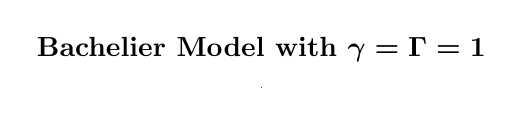
\begin{tikzpicture}[%
font=\footnotesize
]

\begin{axis}[%
width=0.951\figwidth,
height=\figheight,
at={(0\figwidth,0\figheight)},
scale only axis,
xmin=0,
xmax=3,
tick align=outside,
xlabel={$\bar P - p$},
xmajorgrids,
ymin=0,
ymax=1,
ylabel={$T-t$},
ymajorgrids,
zmin=0,
zmax=800,
zlabel={Optimal Rate $\bar u$},
zmajorgrids,
view={50}{40},
axis background/.style={fill=white},
title style={font=\bfseries},
title={Bachelier Model with $\boldsymbol{\gamma = \Gamma = 1}$},
axis x line*=bottom,
axis y line*=left,
axis z line*=left
]

\addplot3[%
surf,
shader=flat corner,draw=black,z buffer=sort,colormap={mymap}{[1pt] rgb(0pt)=(0.2081,0.1663,0.5292); rgb(1pt)=(0.211624,0.189781,0.577676); rgb(2pt)=(0.212252,0.213771,0.626971); rgb(3pt)=(0.2081,0.2386,0.677086); rgb(4pt)=(0.195905,0.264457,0.7279); rgb(5pt)=(0.170729,0.291938,0.779248); rgb(6pt)=(0.125271,0.324243,0.830271); rgb(7pt)=(0.0591333,0.359833,0.868333); rgb(8pt)=(0.0116952,0.38751,0.881957); rgb(9pt)=(0.00595714,0.408614,0.882843); rgb(10pt)=(0.0165143,0.4266,0.878633); rgb(11pt)=(0.0328524,0.443043,0.871957); rgb(12pt)=(0.0498143,0.458571,0.864057); rgb(13pt)=(0.0629333,0.47369,0.855438); rgb(14pt)=(0.0722667,0.488667,0.8467); rgb(15pt)=(0.0779429,0.503986,0.838371); rgb(16pt)=(0.0793476,0.520024,0.831181); rgb(17pt)=(0.0749429,0.537543,0.826271); rgb(18pt)=(0.0640571,0.556986,0.823957); rgb(19pt)=(0.0487714,0.577224,0.822829); rgb(20pt)=(0.0343429,0.596581,0.819852); rgb(21pt)=(0.0265,0.6137,0.8135); rgb(22pt)=(0.0238905,0.628662,0.803762); rgb(23pt)=(0.0230905,0.641786,0.791267); rgb(24pt)=(0.0227714,0.653486,0.776757); rgb(25pt)=(0.0266619,0.664195,0.760719); rgb(26pt)=(0.0383714,0.674271,0.743552); rgb(27pt)=(0.0589714,0.683757,0.725386); rgb(28pt)=(0.0843,0.692833,0.706167); rgb(29pt)=(0.113295,0.7015,0.685857); rgb(30pt)=(0.145271,0.709757,0.664629); rgb(31pt)=(0.180133,0.717657,0.642433); rgb(32pt)=(0.217829,0.725043,0.619262); rgb(33pt)=(0.258643,0.731714,0.595429); rgb(34pt)=(0.302171,0.737605,0.571186); rgb(35pt)=(0.348167,0.742433,0.547267); rgb(36pt)=(0.395257,0.7459,0.524443); rgb(37pt)=(0.44201,0.748081,0.503314); rgb(38pt)=(0.487124,0.749062,0.483976); rgb(39pt)=(0.530029,0.749114,0.466114); rgb(40pt)=(0.570857,0.748519,0.44939); rgb(41pt)=(0.609852,0.747314,0.433686); rgb(42pt)=(0.6473,0.7456,0.4188); rgb(43pt)=(0.683419,0.743476,0.404433); rgb(44pt)=(0.71841,0.741133,0.390476); rgb(45pt)=(0.752486,0.7384,0.376814); rgb(46pt)=(0.785843,0.735567,0.363271); rgb(47pt)=(0.818505,0.732733,0.34979); rgb(48pt)=(0.850657,0.7299,0.336029); rgb(49pt)=(0.882433,0.727433,0.3217); rgb(50pt)=(0.913933,0.725786,0.306276); rgb(51pt)=(0.944957,0.726114,0.288643); rgb(52pt)=(0.973895,0.731395,0.266648); rgb(53pt)=(0.993771,0.745457,0.240348); rgb(54pt)=(0.999043,0.765314,0.216414); rgb(55pt)=(0.995533,0.786057,0.196652); rgb(56pt)=(0.988,0.8066,0.179367); rgb(57pt)=(0.978857,0.827143,0.163314); rgb(58pt)=(0.9697,0.848138,0.147452); rgb(59pt)=(0.962586,0.870514,0.1309); rgb(60pt)=(0.958871,0.8949,0.113243); rgb(61pt)=(0.959824,0.921833,0.0948381); rgb(62pt)=(0.9661,0.951443,0.0755333); rgb(63pt)=(0.9763,0.9831,0.0538)},mesh/rows=25]
table[row sep=crcr, point meta=\thisrow{c}] {%
%
x	y	z	c\\
0	0.01	32.6278781458054	32.6278781458054\\
0	0.0302040816326531	34.0436214822138	34.0436214822138\\
0	0.0504081632653061	35.5293394199211	35.5293394199211\\
0	0.0706122448979592	37.1580840095691	37.1580840095691\\
0	0.0908163265306122	38.9520453232922	38.9520453232922\\
0	0.111020408163265	40.9240326133239	40.9240326133239\\
0	0.131224489795918	43.0842726192078	43.0842726192078\\
0	0.151428571428571	45.4424019894934	45.4424019894934\\
0	0.171632653061224	48.0082361437621	48.0082361437621\\
0	0.191836734693878	50.7921270819487	50.7921270819487\\
0	0.212040816326531	53.8051586279449	53.8051586279449\\
0	0.232244897959184	57.0592705953301	57.0592705953301\\
0	0.252448979591837	60.5673502218759	60.5673502218759\\
0	0.27265306122449	64.3433085971243	64.3433085971243\\
0	0.292857142857143	68.4021509494082	68.4021509494082\\
0	0.313061224489796	72.7600455448047	72.7600455448047\\
0	0.333265306122449	77.43439391991	77.43439391991\\
0	0.353469387755102	82.443904119548	82.443904119548\\
0	0.373673469387755	87.8086680477885	87.8086680477885\\
0	0.393877551020408	93.550243732921	93.550243732921\\
0	0.414081632653061	99.6917431382939	99.6917431382939\\
0	0.434285714285714	106.257926060887	106.257926060887\\
0	0.454489795918367	113.275300615761	113.275300615761\\
0	0.47469387755102	120.772230788653	120.772230788653\\
0	0.494897959183673	128.779051541082	128.779051541082\\
0	0.515102040816326	137.32819196603	137.32819196603\\
0	0.53530612244898	146.454307014064	146.454307014064\\
0	0.555510204081633	156.194418337882	156.194418337882\\
0	0.575714285714286	166.588064835488	166.588064835488\\
0	0.595918367346939	177.677463509538	177.677463509538\\
0	0.616122448979592	189.507681299655	189.507681299655\\
0	0.636326530612245	202.126818589336	202.126818589336\\
0	0.656530612244898	215.586205134772	215.586205134772\\
0	0.676734693877551	229.940609214331	229.940609214331\\
0	0.696938775510204	245.248460850454	245.248460850454\\
0	0.717142857142857	261.57209001353	261.57209001353\\
0	0.73734693877551	278.977980778294	278.977980778294\\
0	0.757551020408163	297.537042468697	297.537042468697\\
0	0.777755102040816	317.324898896306	317.324898896306\\
0	0.797959183673469	338.422196871824	338.422196871824\\
0	0.818163265306122	360.914935247611	360.914935247611\\
0	0.838367346938775	384.89481583336	384.89481583336\\
0	0.858571428571429	410.45961761655	410.45961761655\\
0	0.878775510204082	437.713595814007	437.713595814007\\
0	0.898979591836735	466.767907383741	466.767907383741\\
0	0.919183673469388	497.741064732281	497.741064732281\\
0	0.939387755102041	530.759419470531	530.759419470531\\
0	0.959591836734694	565.957678191312	565.957678191312\\
0	0.979795918367347	603.479452374845	603.479452374845\\
0	1	643.477844666367	643.477844666367\\
0.125	0.01	31.958091902389	31.958091902389\\
0.125	0.0302040816326531	32.8242902165571	32.8242902165571\\
0.125	0.0504081632653061	33.9048445959123	33.9048445959123\\
0.125	0.0706122448979592	35.163909003554	35.163909003554\\
0.125	0.0908163265306122	36.5956282251183	36.5956282251183\\
0.125	0.111020408163265	38.2020205546834	38.2020205546834\\
0.125	0.131224489795918	39.9878892692935	39.9878892692935\\
0.125	0.151428571428571	41.9594956710628	41.9594956710628\\
0.125	0.171632653061224	44.1241554123878	44.1241554123878\\
0.125	0.191836734693878	46.4901115840895	46.4901115840895\\
0.125	0.212040816326531	49.0665049043418	49.0665049043418\\
0.125	0.232244897959184	51.8633830454246	51.8633830454246\\
0.125	0.252448979591837	54.8917282556236	54.8917282556236\\
0.125	0.27265306122449	58.1634951863175	58.1634951863175\\
0.125	0.292857142857143	61.6916556391047	61.6916556391047\\
0.125	0.313061224489796	65.490248897567	65.490248897567\\
0.125	0.333265306122449	69.5744371511391	69.5744371511391\\
0.125	0.353469387755102	73.9605659054028	73.9605659054028\\
0.125	0.373673469387755	78.6662294627833	78.6662294627833\\
0.125	0.393877551020408	83.7103416588195	83.7103416588195\\
0.125	0.414081632653061	89.1132120997202	89.1132120997202\\
0.125	0.434285714285714	94.8966281886601	94.8966281886601\\
0.125	0.454489795918367	101.083943259113	101.083943259113\\
0.125	0.47469387755102	107.700171183767	107.700171183767\\
0.125	0.494897959183673	114.772087787508	114.772087787508\\
0.125	0.515102040816326	122.328339546305	122.328339546305\\
0.125	0.53530612244898	130.399559955141	130.399559955141\\
0.125	0.555510204081633	139.018494058695	139.018494058695\\
0.125	0.575714285714286	148.220131645984	148.220131645984\\
0.125	0.595918367346939	158.041849649497	158.041849649497\\
0.125	0.616122448979592	168.523564327244	168.523564327244\\
0.125	0.636326530612245	179.707893846302	179.707893846302\\
0.125	0.656530612244898	191.640331957175	191.640331957175\\
0.125	0.676734693877551	204.369433332139	204.369433332139\\
0.125	0.696938775510204	217.947011471459	217.947011471459\\
0.125	0.717142857142857	232.42835032236	232.42835032236\\
0.125	0.73734693877551	247.872429252541	247.872429252541\\
0.125	0.757551020408163	264.342163909042	264.342163909042\\
0.125	0.777755102040816	281.904662819036	281.904662819036\\
0.125	0.797959183673469	300.631501191342	300.631501191342\\
0.125	0.818163265306122	320.599012972535	320.599012972535\\
0.125	0.838367346938775	341.888602349043	341.888602349043\\
0.125	0.858571428571429	364.587075966159	364.587075966159\\
0.125	0.878775510204082	388.78699721957	388.78699721957\\
0.125	0.898979591836735	414.587064065227	414.587064065227\\
0.125	0.919183673469388	442.092511889491	442.092511889491\\
0.125	0.939387755102041	471.415543083896	471.415543083896\\
0.125	0.959591836734694	502.675785077982	502.675785077982\\
0.125	0.979795918367347	536.000778699906	536.000778699906\\
0.125	1	571.526498858454	571.526498858454\\
0.25	0.01	31.9548698659926	31.9548698659926\\
0.25	0.0302040816326531	32.725401432364	32.725401432364\\
0.25	0.0504081632653061	33.6438193464945	33.6438193464945\\
0.25	0.0706122448979592	34.7226042513612	34.7226042513612\\
0.25	0.0908163265306122	35.9661893124192	35.9661893124192\\
0.25	0.111020408163265	37.3778726309472	37.3778726309472\\
0.25	0.131224489795918	38.9618284378291	38.9618284378291\\
0.25	0.151428571428571	40.7233539697866	40.7233539697866\\
0.25	0.171632653061224	42.6688018229418	42.6688018229418\\
0.25	0.191836734693878	44.8054996240523	44.8054996240523\\
0.25	0.212040816326531	47.1417027038198	47.1417027038198\\
0.25	0.232244897959184	49.6865771814669	49.6865771814669\\
0.25	0.252448979591837	52.4502051012731	52.4502051012731\\
0.25	0.27265306122449	55.4436050458327	55.4436050458327\\
0.25	0.292857142857143	58.6787639447243	58.6787639447243\\
0.25	0.313061224489796	62.1686774663553	62.1686774663553\\
0.25	0.333265306122449	65.9273974578144	65.9273974578144\\
0.25	0.353469387755102	69.9700855703196	69.9700855703196\\
0.25	0.373673469387755	74.3130726277572	74.3130726277572\\
0.25	0.393877551020408	78.9739235619597	78.9739235619597\\
0.25	0.414081632653061	83.9715079117012	83.9715079117012\\
0.25	0.434285714285714	89.3260759995747	89.3260759995747\\
0.25	0.454489795918367	95.0593409840635	95.0593409840635\\
0.25	0.47469387755102	101.194567046611	101.194567046611\\
0.25	0.494897959183673	107.75666402355	107.75666402355\\
0.25	0.515102040816326	114.772288835469	114.772288835469\\
0.25	0.53530612244898	122.269954105239	122.269954105239\\
0.25	0.555510204081633	130.28014439251	130.28014439251\\
0.25	0.575714285714286	138.835440508537	138.835440508537\\
0.25	0.595918367346939	147.97065241147	147.97065241147\\
0.25	0.616122448979592	157.722961219583	157.722961219583\\
0.25	0.636326530612245	168.132070918694	168.132070918694\\
0.25	0.656530612244898	179.240370380706	179.240370380706\\
0.25	0.676734693877551	191.093106353041	191.093106353041\\
0.25	0.696938775510204	203.738568124066	203.738568124066\\
0.25	0.717142857142857	217.228284617644	217.228284617644\\
0.25	0.73734693877551	231.617234720964	231.617234720964\\
0.25	0.757551020408163	246.964071704	246.964071704\\
0.25	0.777755102040816	263.331362646645	263.331362646645\\
0.25	0.797959183673469	280.785843850893	280.785843850893\\
0.25	0.818163265306122	299.398693280833	299.398693280833\\
0.25	0.838367346938775	319.245821142744	319.245821142744\\
0.25	0.858571428571429	340.408179791718	340.408179791718\\
0.25	0.878775510204082	362.97209423016	362.97209423016\\
0.25	0.898979591836735	387.029614547627	387.029614547627\\
0.25	0.919183673469388	412.678891741064	412.678891741064\\
0.25	0.939387755102041	440.024578449993	440.024578449993\\
0.25	0.959591836734694	469.178256242921	469.178256242921\\
0.25	0.979795918367347	500.25889119971	500.25889119971\\
0.25	1	533.393319650151	533.393319650151\\
0.375	0.01	31.9548697809241	31.9548697809241\\
0.375	0.0302040816326531	32.7237260624826	32.7237260624826\\
0.375	0.0504081632653061	33.6266080756176	33.6266080756176\\
0.375	0.0706122448979592	34.6692573771336	34.6692573771336\\
0.375	0.0908163265306122	35.8587540699031	35.8587540699031\\
0.375	0.111020408163265	37.202058715722	37.202058715722\\
0.375	0.131224489795918	38.7059208527281	38.7059208527281\\
0.375	0.151428571428571	40.3772023150716	40.3772023150716\\
0.375	0.171632653061224	42.2231450639686	42.2231450639686\\
0.375	0.191836734693878	44.2515405224866	44.2515405224866\\
0.375	0.212040816326531	46.4708356863834	46.4708356863834\\
0.375	0.232244897959184	48.8902060942456	48.8902060942456\\
0.375	0.252448979591837	51.519613229844	51.519613229844\\
0.375	0.27265306122449	54.3698556932201	54.3698556932201\\
0.375	0.292857142857143	57.4526189940999	57.4526189940999\\
0.375	0.313061224489796	60.7805265206817	60.7805265206817\\
0.375	0.333265306122449	64.3671930802789	64.3671930802789\\
0.375	0.353469387755102	68.2272818325113	68.2272818325113\\
0.375	0.373673469387755	72.3765651528717	72.3765651528717\\
0.375	0.393877551020408	76.8319898299131	76.8319898299131\\
0.375	0.414081632653061	81.6117469404814	81.6117469404814\\
0.375	0.434285714285714	86.7353467277575	86.7353467277575\\
0.375	0.454489795918367	92.2236988078475	92.2236988078475\\
0.375	0.47469387755102	98.099198042811	98.099198042811\\
0.375	0.494897959183673	104.385816436546	104.385816436546\\
0.375	0.515102040816326	111.109201432422	111.109201432422\\
0.375	0.53530612244898	118.296781016778	118.296781016778\\
0.375	0.555510204081633	125.977876059851	125.977876059851\\
0.375	0.575714285714286	134.183820355123	134.183820355123\\
0.375	0.595918367346939	142.948088849464	142.948088849464\\
0.375	0.616122448979592	152.306434589889	152.306434589889\\
0.375	0.636326530612245	162.297034948252	162.297034948252\\
0.375	0.656530612244898	172.960647723032	172.960647723032\\
0.375	0.676734693877551	184.340777757614	184.340777757614\\
0.375	0.696938775510204	196.483854757268	196.483854757268\\
0.375	0.717142857142857	209.439423032655	209.439423032655\\
0.375	0.73734693877551	223.26034394628	223.26034394628\\
0.375	0.757551020408163	238.003011890006	238.003011890006\\
0.375	0.777755102040816	253.727584676946	253.727584676946\\
0.375	0.797959183673469	270.498229289709	270.498229289709\\
0.375	0.818163265306122	288.383383989653	288.383383989653\\
0.375	0.838367346938775	307.45603785843	307.45603785843\\
0.375	0.858571428571429	327.794028914254	327.794028914254\\
0.375	0.878775510204082	349.480362021034	349.480362021034\\
0.375	0.898979591836735	372.603547889302	372.603547889302\\
0.375	0.919183673469388	397.257964553874	397.257964553874\\
0.375	0.939387755102041	423.544242804939	423.544242804939\\
0.375	0.959591836734694	451.569677146989	451.569677146989\\
0.375	0.979795918367347	481.448663964211	481.448663964211\\
0.375	1	513.303168681999	513.303168681999\\
0.5	0.01	31.954869780924	31.954869780924\\
0.5	0.0302040816326531	32.7237213190093	32.7237213190093\\
0.5	0.0504081632653061	33.6262013408688	33.6262013408688\\
0.5	0.0706122448979592	34.6660748760192	34.6660748760192\\
0.5	0.0908163265306122	35.8479556793739	35.8479556793739\\
0.5	0.111020408163265	37.1773607079571	37.1773607079571\\
0.5	0.131224489795918	38.6605442335418	38.6605442335418\\
0.5	0.151428571428571	40.3043599367312	40.3043599367312\\
0.5	0.171632653061224	42.1162194087248	42.1162194087248\\
0.5	0.191836734693878	44.1041112444042	44.1041112444042\\
0.5	0.212040816326531	46.2766456717106	46.2766456717106\\
0.5	0.232244897959184	48.643107180854	48.643107180854\\
0.5	0.252448979591837	51.2135086296628	51.2135086296628\\
0.5	0.27265306122449	53.9986452461684	53.9986452461684\\
0.5	0.292857142857143	57.0101487847191	57.0101487847191\\
0.5	0.313061224489796	60.2605426177681	60.2605426177681\\
0.5	0.333265306122449	63.7632985921478	63.7632985921478\\
0.5	0.353469387755102	67.532896383907	67.532896383907\\
0.5	0.373673469387755	71.5848859733097	71.5848859733097\\
0.5	0.393877551020408	75.9359537695743	75.9359537695743\\
0.5	0.414081632653061	80.6039928501877	80.6039928501877\\
0.5	0.434285714285714	85.6081777389537	85.6081777389537\\
0.5	0.454489795918367	90.9690441250445	90.9690441250445\\
0.5	0.47469387755102	96.7085739173911	96.7085739173911\\
0.5	0.494897959183673	102.850286031062	102.850286031062\\
0.5	0.515102040816326	109.419333312179	109.419333312179\\
0.5	0.53530612244898	116.442606023557	116.442606023557\\
0.5	0.555510204081633	123.94884233343	123.94884233343\\
0.5	0.575714285714286	131.968746273525	131.968746273525\\
0.5	0.595918367346939	140.535113659847	140.535113659847\\
0.5	0.616122448979592	149.682966499633	149.682966499633\\
0.5	0.636326530612245	159.449696440729	159.449696440729\\
0.5	0.656530612244898	169.875217855241	169.875217855241\\
0.5	0.676734693877551	181.002131187597	181.002131187597\\
0.5	0.696938775510204	192.875897238259	192.875897238259\\
0.5	0.717142857142857	205.545023098369	205.545023098369\\
0.5	0.73734693877551	219.061260497645	219.061260497645\\
0.5	0.757551020408163	233.479817378175	233.479817378175\\
0.5	0.777755102040816	248.859583560351	248.859583560351\\
0.5	0.797959183673469	265.263371424516	265.263371424516\\
0.5	0.818163265306122	282.758172592932	282.758172592932\\
0.5	0.838367346938775	301.415431661813	301.415431661813\\
0.5	0.858571428571429	321.31133810264	321.31133810264\\
0.5	0.878775510204082	342.527137525978	342.527137525978\\
0.5	0.898979591836735	365.149463579989	365.149463579989\\
0.5	0.919183673469388	389.270691839938	389.270691839938\\
0.5	0.939387755102041	414.989317134726	414.989317134726\\
0.5	0.959591836734694	442.410355852065	442.410355852065\\
0.5	0.979795918367347	471.645774865839	471.645774865839\\
0.5	1	502.81494883785	502.81494883785\\
0.625	0.01	31.954869780924	31.954869780924\\
0.625	0.0302040816326531	32.7237213170079	32.7237213170079\\
0.625	0.0504081632653061	33.6261981458795	33.6261981458795\\
0.625	0.0706122448979592	34.66598655804	34.66598655804\\
0.625	0.0908163265306122	35.8473480284754	35.8473480284754\\
0.625	0.111020408163265	37.1751755192253	37.1751755192253\\
0.625	0.131224489795918	38.6550467512355	38.6550467512355\\
0.625	0.151428571428571	40.2932442161499	40.2932442161499\\
0.625	0.171632653061224	42.0967542024371	42.0967542024371\\
0.625	0.191836734693878	44.0732660159472	44.0732660159472\\
0.625	0.212040816326531	46.2311812686409	46.2311812686409\\
0.625	0.232244897959184	48.5796344436852	48.5796344436852\\
0.625	0.252448979591837	51.1285228501553	51.1285228501553\\
0.625	0.27265306122449	53.8885438104162	53.8885438104162\\
0.625	0.292857142857143	56.8712375029794	56.8712375029794\\
0.625	0.313061224489796	60.0890345160046	60.0890345160046\\
0.625	0.333265306122449	63.5553076407712	63.5553076407712\\
0.625	0.353469387755102	67.2844277457016	67.2844277457016\\
0.625	0.373673469387755	71.2918237641868	71.2918237641868\\
0.625	0.393877551020408	75.5940469464862	75.5940469464862\\
0.625	0.414081632653061	80.2088395981023	80.2088395981023\\
0.625	0.434285714285714	85.1552085738765	85.1552085738765\\
0.625	0.454489795918367	90.4535038304191	90.4535038304191\\
0.625	0.47469387755102	96.1255023662231	96.1255023662231\\
0.625	0.494897959183673	102.194497902809	102.194497902809\\
0.625	0.515102040816326	108.685396683698	108.685396683698\\
0.625	0.53530612244898	115.624819792091	115.624819792091\\
0.625	0.555510204081633	123.041212413591	123.041212413591\\
0.625	0.575714285714286	130.964960497408	130.964960497408\\
0.625	0.595918367346939	139.428515298617	139.428515298617\\
0.625	0.616122448979592	148.466526315249	148.466526315249\\
0.625	0.636326530612245	158.115983167439	158.115983167439\\
0.625	0.656530612244898	168.416367001732	168.416367001732\\
0.625	0.676734693877551	179.409812041955	179.409812041955\\
0.625	0.696938775510204	191.141277949068	191.141277949068\\
0.625	0.717142857142857	203.658733696147	203.658733696147\\
0.625	0.73734693877551	217.013353711397	217.013353711397\\
0.625	0.757551020408163	231.259727091913	231.259727091913\\
0.625	0.777755102040816	246.456080744077	246.456080744077\\
0.625	0.797959183673469	262.664517363172	262.664517363172\\
0.625	0.818163265306122	279.951269225235	279.951269225235\\
0.625	0.838367346938775	298.386968828626	298.386968828626\\
0.625	0.858571428571429	318.046937491454	318.046937491454\\
0.625	0.878775510204082	339.011493084264	339.011493084264\\
0.625	0.898979591836735	361.36627815542	361.36627815542\\
0.625	0.919183673469388	385.202609789814	385.202609789814\\
0.625	0.939387755102041	410.617852630243	410.617852630243\\
0.625	0.959591836734694	437.715816585271	437.715816585271\\
0.625	0.979795918367347	466.607180848208	466.607180848208\\
0.625	1	497.409945959173	497.409945959173\\
0.75	0.01	31.954869780924	31.954869780924\\
0.75	0.0302040816326531	32.7237213170077	32.7237213170077\\
0.75	0.0504081632653061	33.6261981378987	33.6261981378987\\
0.75	0.0706122448979592	34.6659854576903	34.6659854576903\\
0.75	0.0908163265306122	35.8473294694509	35.8473294694509\\
0.75	0.111020408163265	37.1750571519442	37.1750571519442\\
0.75	0.131224489795918	38.6546034925561	38.6546034925561\\
0.75	0.151428571428571	40.2920439778025	40.2920439778025\\
0.75	0.171632653061224	42.0941265370898	42.0941265370898\\
0.75	0.191836734693878	44.0683003509599	44.0683003509599\\
0.75	0.212040816326531	46.2227428959571	46.2227428959571\\
0.75	0.232244897959184	48.566387776905	48.566387776905\\
0.75	0.252448979591837	51.1089553366	51.1089553366\\
0.75	0.27265306122449	53.8609871539929	53.8609871539929\\
0.75	0.292857142857143	56.8338849121257	56.8338849121257\\
0.75	0.313061224489796	60.0399537884368	60.0399537884368\\
0.75	0.333265306122449	63.4924503958512	63.4924503958512\\
0.75	0.353469387755102	67.2056352882014	67.2056352882014\\
0.75	0.373673469387755	71.1948300769895	71.1948300769895\\
0.75	0.393877551020408	75.4764792560383	75.4764792560383\\
0.75	0.414081632653061	80.0682168815605	80.0682168815605\\
0.75	0.434285714285714	84.9889383021909	84.9889383021909\\
0.75	0.454489795918367	90.2588771755079	90.2588771755079\\
0.75	0.47469387755102	95.899688045143	95.899688045143\\
0.75	0.494897959183673	101.934534786927	101.934534786927\\
0.75	0.515102040816326	108.388185264825	108.388185264825\\
0.75	0.53530612244898	115.287112568674	115.287112568674\\
0.75	0.555510204081633	122.659603236798	122.659603236798\\
0.75	0.575714285714286	130.535872898033	130.535872898033\\
0.75	0.595918367346939	138.948189800071	138.948189800071\\
0.75	0.616122448979592	147.931006724713	147.931006724713\\
0.75	0.636326530612245	157.52110182591	157.52110182591\\
0.75	0.656530612244898	167.757728963686	167.757728963686\\
0.75	0.676734693877551	178.682778146325	178.682778146325\\
0.75	0.696938775510204	190.340946734924	190.340946734924\\
0.75	0.717142857142857	202.779922108606	202.779922108606\\
0.75	0.73734693877551	216.050576535759	216.050576535759\\
0.75	0.757551020408163	230.207175046641	230.207175046641\\
0.75	0.777755102040816	245.307597155911	245.307597155911\\
0.75	0.797959183673469	261.413573340316	261.413573340316\\
0.75	0.818163265306122	278.590937237076	278.590937237076\\
0.75	0.838367346938775	296.909894592748	296.909894592748\\
0.75	0.858571428571429	316.445310060842	316.445310060842\\
0.75	0.878775510204082	337.27701301931	337.27701301931\\
0.75	0.898979591836735	359.490123656792	359.490123656792\\
0.75	0.919183673469388	383.175400659243	383.175400659243\\
0.75	0.939387755102041	408.429611916802	408.429611916802\\
0.75	0.959591836734694	435.355929764778	435.355929764778\\
0.75	0.979795918367347	464.064352372816	464.064352372816\\
0.75	1	494.672153003082	494.672153003082\\
0.875	0.01	31.954869780924	31.954869780924\\
0.875	0.0302040816326531	32.7237213170077	32.7237213170077\\
0.875	0.0504081632653061	33.6261981378926	33.6261981378926\\
0.875	0.0706122448979592	34.6659854516731	34.6659854516731\\
0.875	0.0908163265306122	35.8473291678466	35.8473291678466\\
0.875	0.111020408163265	37.1750532977935	37.1750532977935\\
0.875	0.131224489795918	38.6545801164966	38.6545801164966\\
0.875	0.151428571428571	40.2919537882264	40.2919537882264\\
0.875	0.171632653061224	42.093867663594	42.093867663594\\
0.875	0.191836734693878	44.0676945859768	44.0676945859768\\
0.875	0.212040816326531	46.2215193620275	46.2215193620275\\
0.875	0.232244897959184	48.5641730163801	48.5641730163801\\
0.875	0.252448979591837	51.1052689735048	51.1052689735048\\
0.875	0.27265306122449	53.8552415951245	53.8552415951245\\
0.875	0.292857142857143	56.8253875680589	56.8253875680589\\
0.875	0.313061224489796	60.0279105922997	60.0279105922997\\
0.875	0.333265306122449	63.4759697447688	63.4759697447688\\
0.875	0.353469387755102	67.1837318304425	67.1837318304425\\
0.875	0.373673469387755	71.1664279913011	71.1664279913011\\
0.875	0.393877551020408	75.4404148239425	75.4404148239425\\
0.875	0.414081632653061	80.0232402536906	80.0232402536906\\
0.875	0.434285714285714	84.9337144214708	84.9337144214708\\
0.875	0.454489795918367	90.191985855654	90.191985855654\\
0.875	0.47469387755102	95.8196232217524	95.8196232217524\\
0.875	0.494897959183673	101.839702966629	101.839702966629\\
0.875	0.515102040816326	108.276903199783	108.276903199783\\
0.875	0.53530612244898	115.157604181837	115.157604181837\\
0.875	0.555510204081633	122.50999581934	122.50999581934\\
0.875	0.575714285714286	130.36419259547	130.36419259547\\
0.875	0.595918367346939	138.752356398134	138.752356398134\\
0.875	0.616122448979592	147.708827740586	147.708827740586\\
0.875	0.636326530612245	157.270265905026	157.270265905026\\
0.875	0.656530612244898	167.475798577039	167.475798577039\\
0.875	0.676734693877551	178.367181578194	178.367181578194\\
0.875	0.696938775510204	189.988969346018	189.988969346018\\
0.875	0.717142857142857	202.388696854915	202.388696854915\\
0.875	0.73734693877551	215.617073718759	215.617073718759\\
0.875	0.757551020408163	229.728191265948	229.728191265948\\
0.875	0.777755102040816	244.779743430996	244.779743430996\\
0.875	0.797959183673469	260.833262363355	260.833262363355\\
0.875	0.818163265306122	277.954369714474	277.954369714474\\
0.875	0.838367346938775	296.213044628286	296.213044628286\\
0.875	0.858571428571429	315.683909528657	315.683909528657\\
0.875	0.878775510204082	336.446534870101	336.446534870101\\
0.875	0.898979591836735	358.585764095644	358.585764095644\\
0.875	0.919183673469388	382.192060128266	382.192060128266\\
0.875	0.939387755102041	407.361874810391	407.361874810391\\
0.875	0.959591836734694	434.198042799644	434.198042799644\\
0.875	0.979795918367347	462.810201529031	462.810201529031\\
0.875	1	493.315238946142	493.315238946142\\
1	0.01	31.954869780924	31.954869780924\\
1	0.0302040816326531	32.7237213170077	32.7237213170077\\
1	0.0504081632653061	33.6261981378926	33.6261981378926\\
1	0.0706122448979592	34.6659854516589	34.6659854516589\\
1	0.0908163265306122	35.8473291652732	35.8473291652732\\
1	0.111020408163265	37.175053223282	37.175053223282\\
1	0.131224489795918	38.6545793195952	38.6545793195952\\
1	0.151428571428571	40.2919491252492	40.2919491252492\\
1	0.171632653061224	42.0938492562059	42.0938492562059\\
1	0.191836734693878	44.0676391925035	44.0676391925035\\
1	0.212040816326531	46.2213822284257	46.2213822284257\\
1	0.232244897959184	48.5638794121046	48.5638794121046\\
1	0.252448979591837	51.104706416315	51.104706416315\\
1	0.27265306122449	53.8542533511859	53.8542533511859\\
1	0.292857142857143	56.8237676234172	56.8237676234172\\
1	0.313061224489796	60.0254000244973	60.0254000244973\\
1	0.333265306122449	63.4722542806491	63.4722542806491\\
1	0.353469387755102	67.1784403244687	67.1784403244687\\
1	0.373673469387755	71.1591315616295	71.1591315616295\\
1	0.393877551020408	75.4306264134526	75.4306264134526\\
1	0.414081632653061	80.0104144227013	80.0104144227013\\
1	0.434285714285714	84.9172472183439	84.9172472183439\\
1	0.454489795918367	90.1712146463818	90.1712146463818\\
1	0.47469387755102	95.7938263884216	95.7938263884216\\
1	0.494897959183673	101.808099407353	101.808099407353\\
1	0.515102040816326	108.238651580008	108.238651580008\\
1	0.53530612244898	115.111801899751	115.111801899751\\
1	0.555510204081633	122.455677657407	122.455677657407\\
1	0.575714285714286	130.300329036588	130.300329036588\\
1	0.595918367346939	138.677851589325	138.677851589325\\
1	0.616122448979592	147.622517089872	147.622517089872\\
1	0.636326530612245	157.170913298758	157.170913298758\\
1	0.656530612244898	167.362093205572	167.362093205572\\
1	0.676734693877551	178.23773435783	178.23773435783\\
1	0.696938775510204	189.842308924564	189.842308924564\\
1	0.717142857142857	202.223265187306	202.223265187306\\
1	0.73734693877551	215.431221197929	215.431221197929\\
1	0.757551020408163	229.52017139267	229.52017139267\\
1	0.777755102040816	244.547707004687	244.547707004687\\
1	0.797959183673469	260.575251173998	260.575251173998\\
1	0.818163265306122	277.66830971378	277.66830971378\\
1	0.838367346938775	295.896738556039	295.896738556039\\
1	0.858571428571429	315.335028967895	315.335028967895\\
1	0.878775510204082	336.062611702353	336.062611702353\\
1	0.898979591836735	358.164181324848	358.164181324848\\
1	0.919183673469388	381.730042039304	381.730042039304\\
1	0.939387755102041	406.856476425298	406.856476425298\\
1	0.959591836734694	433.64613859155	433.64613859155\\
1	0.979795918367347	462.208473350695	462.208473350695\\
1	1	492.660163126609	492.660163126609\\
1.125	0.01	31.954869780924	31.954869780924\\
1.125	0.0302040816326531	32.7237213170077	32.7237213170077\\
1.125	0.0504081632653061	33.6261981378926	33.6261981378926\\
1.125	0.0706122448979592	34.6659854516589	34.6659854516589\\
1.125	0.0908163265306122	35.8473291652618	35.8473291652618\\
1.125	0.111020408163265	37.1750532224341	37.1750532224341\\
1.125	0.131224489795918	38.6545793021778	38.6545793021778\\
1.125	0.151428571428571	40.2919489606909	40.2919489606909\\
1.125	0.171632653061224	42.093848318911	42.093848318911\\
1.125	0.191836734693878	44.0676354248081	44.0676354248081\\
1.125	0.212040816326531	46.2213704383975	46.2213704383975\\
1.125	0.232244897959184	48.5638487836556	48.5638487836556\\
1.125	0.252448979591837	51.1046373929295	51.1046373929295\\
1.125	0.27265306122449	53.8541141556937	53.8541141556937\\
1.125	0.292857142857143	56.8235106862415	56.8235106862415\\
1.125	0.313061224489796	60.0249585432244	60.0249585432244\\
1.125	0.333265306122449	63.4715390609691	63.4715390609691\\
1.125	0.353469387755102	67.1773369816401	67.1773369816401\\
1.125	0.373673469387755	71.1574981047623	71.1574981047623\\
1.125	0.393877551020408	75.4282911951388	75.4282911951388\\
1.125	0.414081632653061	80.0071744121094	80.0071744121094\\
1.125	0.434285714285714	84.9128665433309	84.9128665433309\\
1.125	0.454489795918367	90.1654233458401	90.1654233458401\\
1.125	0.47469387755102	95.7863193169572	95.7863193169572\\
1.125	0.494897959183673	101.798535238216	101.798535238216\\
1.125	0.515102040816326	108.226651857433	108.226651857433\\
1.125	0.53530612244898	115.096950097519	115.096950097519\\
1.125	0.555510204081633	122.43751820591	122.43751820591\\
1.125	0.575714285714286	130.278366285652	130.278366285652\\
1.125	0.595918367346939	138.651548678389	138.651548678389\\
1.125	0.616122448979592	147.591294700783	147.591294700783\\
1.125	0.636326530612245	157.134148269431	157.134148269431\\
1.125	0.656530612244898	167.319116985181	167.319116985181\\
1.125	0.676734693877551	178.187831286023	178.187831286023\\
1.125	0.696938775510204	189.784714318617	189.784714318617\\
1.125	0.717142857142857	202.157163222061	202.157163222061\\
1.125	0.73734693877551	215.35574256402	215.35574256402\\
1.125	0.757551020408163	229.434390718818	229.434390718818\\
1.125	0.777755102040816	244.450640029917	244.450640029917\\
1.125	0.797959183673469	260.465851655434	260.465851655434\\
1.125	0.818163265306122	277.545466055293	277.545466055293\\
1.125	0.838367346938775	295.759270142463	295.759270142463\\
1.125	0.858571428571429	315.181682188787	315.181682188787\\
1.125	0.878775510204082	335.892055648394	335.892055648394\\
1.125	0.898979591836735	357.97500313899	357.97500313899\\
1.125	0.919183673469388	381.520741903582	381.520741903582\\
1.125	0.939387755102041	406.625462162993	406.625462162993\\
1.125	0.959591836734694	433.391719862953	433.391719862953\\
1.125	0.979795918367347	461.928855419231	461.928855419231\\
1.125	1	492.353440170419	492.353440170419\\
1.25	0.01	31.954869780924	31.954869780924\\
1.25	0.0302040816326531	32.7237213170077	32.7237213170077\\
1.25	0.0504081632653061	33.6261981378926	33.6261981378926\\
1.25	0.0706122448979592	34.6659854516589	34.6659854516589\\
1.25	0.0908163265306122	35.8473291652618	35.8473291652618\\
1.25	0.111020408163265	37.1750532224285	37.1750532224285\\
1.25	0.131224489795918	38.6545793019352	38.6545793019352\\
1.25	0.151428571428571	40.2919489567498	40.2919489567498\\
1.25	0.171632653061224	42.0938482849271	42.0938482849271\\
1.25	0.191836734693878	44.0676352352647	44.0676352352647\\
1.25	0.212040816326531	46.2213696651964	46.2213696651964\\
1.25	0.232244897959184	48.5638462833909	48.5638462833909\\
1.25	0.252448979591837	51.1046306217078	51.1046306217078\\
1.25	0.27265306122449	53.8540981892792	53.8540981892792\\
1.25	0.292857142857143	56.8234769675162	56.8234769675162\\
1.25	0.313061224489796	60.0248934119626	60.0248934119626\\
1.25	0.333265306122449	63.4714221372942	63.4714221372942\\
1.25	0.353469387755102	67.1771394758599	67.1771394758599\\
1.25	0.373673469387755	71.157181117374	71.157181117374\\
1.25	0.393877551020408	75.4278040566956	75.4278040566956\\
1.25	0.414081632653061	80.0064530972407	80.0064530972407\\
1.25	0.434285714285714	84.9118321789371	84.9118321789371\\
1.25	0.454489795918367	90.1639808215474	90.1639808215474\\
1.25	0.47469387755102	95.7843559966671	95.7843559966671\\
1.25	0.494897959183673	101.79591976489	101.79591976489\\
1.25	0.515102040816326	108.223233038738	108.223233038738\\
1.25	0.53530612244898	115.092555857162	115.092555857162\\
1.25	0.555510204081633	122.431954584023	122.431954584023\\
1.25	0.575714285714286	130.27141647101	130.27141647101\\
1.25	0.595918367346939	138.64297205533	138.64297205533\\
1.25	0.616122448979592	147.580825894147	147.580825894147\\
1.25	0.636326530612245	157.121496171539	157.121496171539\\
1.25	0.656530612244898	167.303963749652	167.303963749652\\
1.25	0.676734693877551	178.169831274049	178.169831274049\\
1.25	0.696938775510204	189.763492984057	189.763492984057\\
1.25	0.717142857142857	202.13231592244	202.13231592244\\
1.25	0.73734693877551	215.326833285076	215.326833285076\\
1.25	0.757551020408163	229.400950700748	229.400950700748\\
1.25	0.777755102040816	244.412166283832	244.412166283832\\
1.25	0.797959183673469	260.421805358785	260.421805358785\\
1.25	0.818163265306122	277.495270815175	277.495270815175\\
1.25	0.838367346938775	295.702310115737	295.702310115737\\
1.25	0.858571428571429	315.117300047875	315.117300047875\\
1.25	0.878775510204082	335.819550381465	335.819550381465\\
1.25	0.898979591836735	357.893627672925	357.893627672925\\
1.25	0.919183673469388	381.429700537805	381.429700537805\\
1.25	0.939387755102041	406.523907801764	406.523907801764\\
1.25	0.959591836734694	433.278751033192	433.278751033192\\
1.25	0.979795918367347	461.803513060311	461.803513060311\\
1.25	1	492.214704181668	492.214704181668\\
1.375	0.01	31.954869780924	31.954869780924\\
1.375	0.0302040816326531	32.7237213170077	32.7237213170077\\
1.375	0.0504081632653061	33.6261981378926	33.6261981378926\\
1.375	0.0706122448979592	34.6659854516589	34.6659854516589\\
1.375	0.0908163265306122	35.8473291652618	35.8473291652618\\
1.375	0.111020408163265	37.1750532224284	37.1750532224284\\
1.375	0.131224489795918	38.654579301933	38.654579301933\\
1.375	0.151428571428571	40.2919489566861	40.2919489566861\\
1.375	0.171632653061224	42.0938482840535	42.0938482840535\\
1.375	0.191836734693878	44.0676352282414	44.0676352282414\\
1.375	0.212040816326531	46.2213696266787	46.2213696266787\\
1.375	0.232244897959184	48.5638461243433	48.5638461243433\\
1.375	0.252448979591837	51.1046300928282	51.1046300928282\\
1.375	0.27265306122449	53.8540967040792	53.8540967040792\\
1.375	0.292857142857143	56.8234733216134	56.8234733216134\\
1.375	0.313061224489796	60.024885384532	60.024885384532\\
1.375	0.333265306122449	63.4714059721966	63.4714059721966\\
1.375	0.353469387755102	67.1771092506552	67.1771092506552\\
1.375	0.373673469387755	71.1571280163238	71.1571280163238\\
1.375	0.393877551020408	75.4277155683194	75.4277155683194\\
1.375	0.414081632653061	80.0063121582948	80.0063121582948\\
1.375	0.434285714285714	84.9116162855632	84.9116162855632\\
1.375	0.454489795918367	90.1636611256504	90.1636611256504\\
1.375	0.47469387755102	95.783896402065	95.783896402065\\
1.375	0.494897959183673	101.795276034029	101.795276034029\\
1.375	0.515102040816326	108.222351917148	108.222351917148\\
1.375	0.53530612244898	115.091374219591	115.091374219591\\
1.375	0.555510204081633	122.430398603411	122.430398603411\\
1.375	0.575714285714286	130.269400809205	130.269400809205\\
1.375	0.595918367346939	138.640399072641	138.640399072641\\
1.375	0.616122448979592	147.57758487346	147.57758487346\\
1.375	0.636326530612245	157.11746255169	157.11746255169\\
1.375	0.656530612244898	167.298998362034	167.298998362034\\
1.375	0.676734693877551	178.163779575895	178.163779575895\\
1.375	0.696938775510204	189.756184281556	189.756184281556\\
1.375	0.717142857142857	202.123562576583	202.123562576583\\
1.375	0.73734693877551	215.316429893069	215.316429893069\\
1.375	0.757551020408163	229.388673245733	229.388673245733\\
1.375	0.777755102040816	244.397771245663	244.397771245663\\
1.375	0.797959183673469	260.405028778582	260.405028778582\\
1.375	0.818163265306122	277.475827306386	277.475827306386\\
1.375	0.838367346938775	295.679891814407	295.679891814407\\
1.375	0.858571428571429	315.091575494802	315.091575494802\\
1.375	0.878775510204082	335.790163328828	335.790163328828\\
1.375	0.898979591836735	357.8601958079	357.8601958079\\
1.375	0.919183673469388	381.391814115541	381.391814115541\\
1.375	0.939387755102041	406.4811281799	406.4811281799\\
1.375	0.959591836734694	433.230609099921	433.230609099921\\
1.375	0.979795918367347	461.749507547705	461.749507547705\\
1.375	1	492.154299855691	492.154299855691\\
1.5	0.01	31.954869780924	31.954869780924\\
1.5	0.0302040816326531	32.7237213170077	32.7237213170077\\
1.5	0.0504081632653061	33.6261981378926	33.6261981378926\\
1.5	0.0706122448979592	34.6659854516589	34.6659854516589\\
1.5	0.0908163265306122	35.8473291652618	35.8473291652618\\
1.5	0.111020408163265	37.1750532224284	37.1750532224284\\
1.5	0.131224489795918	38.654579301933	38.654579301933\\
1.5	0.151428571428571	40.2919489566854	40.2919489566854\\
1.5	0.171632653061224	42.0938482840376	42.0938482840376\\
1.5	0.191836734693878	44.0676352280504	44.0676352280504\\
1.5	0.212040816326531	46.2213696252257	46.2213696252257\\
1.5	0.232244897959184	48.5638461164843	48.5638461164843\\
1.5	0.252448979591837	51.1046300600432	51.1046300600432\\
1.5	0.27265306122449	53.8540965924037	53.8540965924037\\
1.5	0.292857142857143	56.8234729978553	56.8234729978553\\
1.5	0.313061224489796	60.0248845606634	60.0248845606634\\
1.5	0.333265306122449	63.4714040883488	63.4714040883488\\
1.5	0.353469387755102	67.1771053092277	67.1771053092277\\
1.5	0.373673469387755	71.1571203627625	71.1571203627625\\
1.5	0.393877551020408	75.4277016174639	75.4277016174639\\
1.5	0.414081632653061	80.0062880682552	80.0062880682552\\
1.5	0.434285714285714	84.9115765835134	84.9115765835134\\
1.5	0.454489795918367	90.1635982915487	90.1635982915487\\
1.5	0.47469387755102	95.783800417161	95.783800417161\\
1.5	0.494897959183673	101.795133901179	101.795133901179\\
1.5	0.515102040816326	108.222147159602	108.222147159602\\
1.5	0.53530612244898	115.091086364205	115.091086364205\\
1.5	0.555510204081633	122.430002653268	122.430002653268\\
1.5	0.575714285714286	130.268866709611	130.268866709611\\
1.5	0.595918367346939	138.639691173363	138.639691173363\\
1.5	0.616122448979592	147.576661389071	147.576661389071\\
1.5	0.636326530612245	157.116275020909	157.116275020909\\
1.5	0.656530612244898	167.297491106106	167.297491106106\\
1.5	0.676734693877551	178.161889155324	178.161889155324\\
1.5	0.696938775510204	189.753838949815	189.753838949815\\
1.5	0.717142857142857	202.120681728926	202.120681728926\\
1.5	0.73734693877551	215.312923508073	215.312923508073\\
1.5	0.757551020408163	229.384441316827	229.384441316827\\
1.5	0.777755102040816	244.392703199574	244.392703199574\\
1.5	0.797959183673469	260.399002877362	260.399002877362\\
1.5	0.818163265306122	277.468710029449	277.468710029449\\
1.5	0.838367346938775	295.671537216813	295.671537216813\\
1.5	0.858571428571429	315.081824537855	315.081824537855\\
1.5	0.878775510204082	335.778843178885	335.778843178885\\
1.5	0.898979591836735	357.847119099152	357.847119099152\\
1.5	0.919183673469388	381.376778172371	381.376778172371\\
1.5	0.939387755102041	406.463914194291	406.463914194291\\
1.5	0.959591836734694	433.210981259207	433.210981259207\\
1.5	0.979795918367347	461.727212107831	461.727212107831\\
1.5	1	492.129064154936	492.129064154936\\
1.625	0.01	31.954869780924	31.954869780924\\
1.625	0.0302040816326531	32.7237213170077	32.7237213170077\\
1.625	0.0504081632653061	33.6261981378926	33.6261981378926\\
1.625	0.0706122448979592	34.6659854516589	34.6659854516589\\
1.625	0.0908163265306122	35.8473291652618	35.8473291652618\\
1.625	0.111020408163265	37.1750532224284	37.1750532224284\\
1.625	0.131224489795918	38.654579301933	38.654579301933\\
1.625	0.151428571428571	40.2919489566854	40.2919489566854\\
1.625	0.171632653061224	42.0938482840374	42.0938482840374\\
1.625	0.191836734693878	44.0676352280466	44.0676352280466\\
1.625	0.212040816326531	46.2213696251843	46.2213696251843\\
1.625	0.232244897959184	48.5638461161834	48.5638461161834\\
1.625	0.252448979591837	51.1046300584343	51.1046300584343\\
1.625	0.27265306122449	53.8540965856329	53.8540965856329\\
1.625	0.292857142857143	56.8234729743037	56.8234729743037\\
1.625	0.313061224489796	60.0248844904327	60.0248844904327\\
1.625	0.333265306122449	63.4714039037669	63.4714039037669\\
1.625	0.353469387755102	67.1771048724016	67.1771048724016\\
1.625	0.373673469387755	71.1571194161066	71.1571194161066\\
1.625	0.393877551020408	75.4276997134974	75.4276997134974\\
1.625	0.414081632653061	80.0062844757053	80.0062844757053\\
1.625	0.434285714285714	84.9115701677355	84.9115701677355\\
1.625	0.454489795918367	90.1635873683336	90.1635873683336\\
1.625	0.47469387755102	95.7837825800016	95.7837825800016\\
1.625	0.494897959183673	101.79510582293	101.79510582293\\
1.625	0.515102040816326	108.222104370134	108.222104370134\\
1.625	0.53530612244898	115.091023006089	115.091023006089\\
1.625	0.555510204081633	122.429911217806	122.429911217806\\
1.625	0.575714285714286	130.268737755557	130.268737755557\\
1.625	0.595918367346939	138.639513030632	138.639513030632\\
1.625	0.616122448979592	147.576419849514	147.576419849514\\
1.625	0.636326530612245	157.115953017993	157.115953017993\\
1.625	0.656530612244898	167.297068384991	167.297068384991\\
1.625	0.676734693877551	178.161341934474	178.161341934474\\
1.625	0.696938775510204	189.753139574956	189.753139574956\\
1.625	0.717142857142857	202.119798319768	202.119798319768\\
1.625	0.73734693877551	215.311819597885	215.311819597885\\
1.625	0.757551020408163	229.383075484642	229.383075484642\\
1.625	0.777755102040816	244.391028694475	244.391028694475\\
1.625	0.797959183673469	260.396967234043	260.396967234043\\
1.625	0.818163265306122	277.466254673981	277.466254673981\\
1.625	0.838367346938775	295.668597061309	295.668597061309\\
1.625	0.858571428571429	315.078327562516	315.078327562516\\
1.625	0.878775510204082	335.774709999724	335.774709999724\\
1.625	0.898979591836735	357.842262519498	357.842262519498\\
1.625	0.919183673469388	381.371102716093	381.371102716093\\
1.625	0.939387755102041	406.45731561853	406.45731561853\\
1.625	0.959591836734694	433.203346044238	433.203346044238\\
1.625	0.979795918367347	461.718416921539	461.718416921539\\
1.625	1	492.118975289253	492.118975289253\\
1.75	0.01	31.954869780924	31.954869780924\\
1.75	0.0302040816326531	32.7237213170077	32.7237213170077\\
1.75	0.0504081632653061	33.6261981378926	33.6261981378926\\
1.75	0.0706122448979592	34.6659854516589	34.6659854516589\\
1.75	0.0908163265306122	35.8473291652618	35.8473291652618\\
1.75	0.111020408163265	37.1750532224284	37.1750532224284\\
1.75	0.131224489795918	38.654579301933	38.654579301933\\
1.75	0.151428571428571	40.2919489566854	40.2919489566854\\
1.75	0.171632653061224	42.0938482840374	42.0938482840374\\
1.75	0.191836734693878	44.0676352280465	44.0676352280465\\
1.75	0.212040816326531	46.2213696251834	46.2213696251834\\
1.75	0.232244897959184	48.5638461161745	48.5638461161745\\
1.75	0.252448979591837	51.1046300583719	51.1046300583719\\
1.75	0.27265306122449	53.8540965853025	53.8540965853025\\
1.75	0.292857142857143	56.823472972903	56.823472972903\\
1.75	0.313061224489796	60.0248844854701	60.0248844854701\\
1.75	0.333265306122449	63.4714038885921	63.4714038885921\\
1.75	0.353469387755102	67.1771048313396	67.1771048313396\\
1.75	0.373673469387755	71.157119315833	71.157119315833\\
1.75	0.393877551020408	75.427699489031	75.427699489031\\
1.75	0.414081632653061	80.0062840092507	80.0062840092507\\
1.75	0.434285714285714	84.9115692586083	84.9115692586083\\
1.75	0.454489795918367	90.1635856923374	90.1635856923374\\
1.75	0.47469387755102	95.7837796368735	95.7837796368735\\
1.75	0.494897959183673	101.795100870792	101.795100870792\\
1.75	0.515102040816326	108.222096346243	108.222096346243\\
1.75	0.53530612244898	115.091010433549	115.091010433549\\
1.75	0.555510204081633	122.429892098205	122.429892098205\\
1.75	0.575714285714286	130.268709447802	130.268709447802\\
1.75	0.595918367346939	138.639472116455	138.639472116455\\
1.75	0.616122448979592	147.576361986299	147.576361986299\\
1.75	0.636326530612245	157.115872779646	157.115872779646\\
1.75	0.656530612244898	167.296959091637	167.296959091637\\
1.75	0.676734693877551	178.161195471758	178.161195471758\\
1.75	0.696938775510204	189.752946203655	189.752946203655\\
1.75	0.717142857142857	202.119546476364	202.119546476364\\
1.75	0.73734693877551	215.311495686631	215.311495686631\\
1.75	0.757551020408163	229.382663661531	229.382663661531\\
1.75	0.777755102040816	244.390510643393	244.390510643393\\
1.75	0.797959183673469	260.396321935238	260.396321935238\\
1.75	0.818163265306122	277.465458164829	277.465458164829\\
1.75	0.838367346938775	295.667622189237	295.667622189237\\
1.75	0.858571428571429	315.077143729768	315.077143729768\\
1.75	0.878775510204082	335.773282899535	335.773282899535\\
1.75	0.898979591836735	357.840553863098	357.840553863098\\
1.75	0.919183673469388	381.369069949835	381.369069949835\\
1.75	0.939387755102041	406.454911630295	406.454911630295\\
1.75	0.959591836734694	433.200518858171	433.200518858171\\
1.75	0.979795918367347	461.715109380027	461.715109380027\\
1.75	1	492.115124720948	492.115124720948\\
1.875	0.01	31.954869780924	31.954869780924\\
1.875	0.0302040816326531	32.7237213170077	32.7237213170077\\
1.875	0.0504081632653061	33.6261981378926	33.6261981378926\\
1.875	0.0706122448979592	34.6659854516589	34.6659854516589\\
1.875	0.0908163265306122	35.8473291652618	35.8473291652618\\
1.875	0.111020408163265	37.1750532224284	37.1750532224284\\
1.875	0.131224489795918	38.654579301933	38.654579301933\\
1.875	0.151428571428571	40.2919489566854	40.2919489566854\\
1.875	0.171632653061224	42.0938482840374	42.0938482840374\\
1.875	0.191836734693878	44.0676352280465	44.0676352280465\\
1.875	0.212040816326531	46.2213696251834	46.2213696251834\\
1.875	0.232244897959184	48.5638461161743	48.5638461161743\\
1.875	0.252448979591837	51.10463005837	51.10463005837\\
1.875	0.27265306122449	53.8540965852896	53.8540965852896\\
1.875	0.292857142857143	56.823472972835	56.823472972835\\
1.875	0.313061224489796	60.0248844851799	60.0248844851799\\
1.875	0.333265306122449	63.4714038875471	63.4714038875471\\
1.875	0.353469387755102	67.1771048280712	67.1771048280712\\
1.875	0.373673469387755	71.1571193067523	71.1571193067523\\
1.875	0.393877551020408	75.4276994662096	75.4276994662096\\
1.875	0.414081632653061	80.0062839566108	80.0062839566108\\
1.875	0.434285714285714	84.9115691458393	84.9115691458393\\
1.875	0.454489795918367	90.1635854657651	90.1635854657651\\
1.875	0.47469387755102	95.7837792064549	95.7837792064549\\
1.875	0.494897959183673	101.795100092406	101.795100092406\\
1.875	0.515102040816326	108.222094998487	108.222094998487\\
1.875	0.53530612244898	115.09100818833	115.09100818833\\
1.875	0.555510204081633	122.429888484516	122.429888484516\\
1.875	0.575714285714286	130.268703808214	130.268703808214\\
1.875	0.595918367346939	138.639463555968	138.639463555968\\
1.875	0.616122448979592	147.576349313324	147.576349313324\\
1.875	0.636326530612245	157.115854439029	157.115854439029\\
1.875	0.656530612244898	167.296933089718	167.296933089718\\
1.875	0.676734693877551	178.161159293542	178.161159293542\\
1.875	0.696938775510204	189.752896722248	189.752896722248\\
1.875	0.717142857142857	202.119479854866	202.119479854866\\
1.875	0.73734693877551	215.311407272694	215.311407272694\\
1.875	0.757551020408163	229.382547874803	229.382547874803\\
1.875	0.777755102040816	244.390360856055	244.390360856055\\
1.875	0.797959183673469	260.396130345817	260.396130345817\\
1.875	0.818163265306122	277.46521566544	277.46521566544\\
1.875	0.838367346938775	295.66731822634	295.66731822634\\
1.875	0.858571428571429	315.076766158503	315.076766158503\\
1.875	0.878775510204082	335.772817831606	335.772817831606\\
1.875	0.898979591836735	357.839985508138	357.839985508138\\
1.875	0.919183673469388	381.368380450096	381.368380450096\\
1.875	0.939387755102041	406.454080888454	406.454080888454\\
1.875	0.959591836734694	433.199524357955	433.199524357955\\
1.875	0.979795918367347	461.713925999298	461.713925999298\\
1.875	1	492.113724536806	492.113724536806\\
2	0.01	31.954869780924	31.954869780924\\
2	0.0302040816326531	32.7237213170077	32.7237213170077\\
2	0.0504081632653061	33.6261981378926	33.6261981378926\\
2	0.0706122448979592	34.6659854516589	34.6659854516589\\
2	0.0908163265306122	35.8473291652618	35.8473291652618\\
2	0.111020408163265	37.1750532224284	37.1750532224284\\
2	0.131224489795918	38.654579301933	38.654579301933\\
2	0.151428571428571	40.2919489566854	40.2919489566854\\
2	0.171632653061224	42.0938482840374	42.0938482840374\\
2	0.191836734693878	44.0676352280465	44.0676352280465\\
2	0.212040816326531	46.2213696251834	46.2213696251834\\
2	0.232244897959184	48.5638461161743	48.5638461161743\\
2	0.252448979591837	51.1046300583699	51.1046300583699\\
2	0.27265306122449	53.8540965852891	53.8540965852891\\
2	0.292857142857143	56.8234729728323	56.8234729728323\\
2	0.313061224489796	60.0248844851658	60.0248844851658\\
2	0.333265306122449	63.4714038874869	63.4714038874869\\
2	0.353469387755102	67.1771048278512	67.1771048278512\\
2	0.373673469387755	71.1571193060502	71.1571193060502\\
2	0.393877551020408	75.4276994642115	75.4276994642115\\
2	0.414081632653061	80.0062839514547	80.0062839514547\\
2	0.434285714285714	84.911569133612	84.911569133612\\
2	0.454489795918367	90.1635854388167	90.1635854388167\\
2	0.47469387755102	95.7837791507433	95.7837791507433\\
2	0.494897959183673	101.795099983527	101.795099983527\\
2	0.515102040816326	108.222094796009	108.222094796009\\
2	0.53530612244898	115.091007828028	115.091007828028\\
2	0.555510204081633	122.429887868087	122.429887868087\\
2	0.575714285714286	130.268702790073	130.268702790073\\
2	0.595918367346939	138.639461926729	138.639461926729\\
2	0.616122448979592	147.576346779626	147.576346779626\\
2	0.636326530612245	157.115850599396	157.115850599396\\
2	0.656530612244898	167.296927406179	167.296927406179\\
2	0.676734693877551	178.161151058825	178.161151058825\\
2	0.696938775510204	189.752885022356	189.752885022356\\
2	0.717142857142857	202.119463526941	202.119463526941\\
2	0.73734693877551	215.311384858076	215.311384858076\\
2	0.757551020408163	229.382517567251	229.382517567251\\
2	0.777755102040816	244.390320445105	244.390320445105\\
2	0.797959183673469	260.39607715529	260.39607715529\\
2	0.818163265306122	277.465146487105	277.465146487105\\
2	0.838367346938775	295.667229248763	295.667229248763\\
2	0.858571428571429	315.076652891093	315.076652891093\\
2	0.878775510204082	335.77267502387	335.77267502387\\
2	0.898979591836735	357.839807064146	357.839807064146\\
2	0.919183673469388	381.368159338129	381.368159338129\\
2	0.939387755102041	406.453809045791	406.453809045791\\
2	0.959591836734694	433.199192590725	433.199192590725\\
2	0.979795918367347	461.713523877292	461.713523877292\\
2	1	492.113240283121	492.113240283121\\
2.125	0.01	31.954869780924	31.954869780924\\
2.125	0.0302040816326531	32.7237213170077	32.7237213170077\\
2.125	0.0504081632653061	33.6261981378926	33.6261981378926\\
2.125	0.0706122448979592	34.6659854516589	34.6659854516589\\
2.125	0.0908163265306122	35.8473291652618	35.8473291652618\\
2.125	0.111020408163265	37.1750532224284	37.1750532224284\\
2.125	0.131224489795918	38.654579301933	38.654579301933\\
2.125	0.151428571428571	40.2919489566854	40.2919489566854\\
2.125	0.171632653061224	42.0938482840374	42.0938482840374\\
2.125	0.191836734693878	44.0676352280465	44.0676352280465\\
2.125	0.212040816326531	46.2213696251834	46.2213696251834\\
2.125	0.232244897959184	48.5638461161743	48.5638461161743\\
2.125	0.252448979591837	51.1046300583699	51.1046300583699\\
2.125	0.27265306122449	53.8540965852891	53.8540965852891\\
2.125	0.292857142857143	56.8234729728322	56.8234729728322\\
2.125	0.313061224489796	60.0248844851653	60.0248844851653\\
2.125	0.333265306122449	63.471403887484	63.471403887484\\
2.125	0.353469387755102	67.1771048278387	67.1771048278387\\
2.125	0.373673469387755	71.1571193060039	71.1571193060039\\
2.125	0.393877551020408	75.427699464061	75.427699464061\\
2.125	0.414081632653061	80.0062839510169	80.0062839510169\\
2.125	0.434285714285714	84.9115691324544	84.9115691324544\\
2.125	0.454489795918367	90.163585436	90.163585436\\
2.125	0.47469387755102	95.7837791443686	95.7837791443686\\
2.125	0.494897959183673	101.79509996999	101.79509996999\\
2.125	0.515102040816326	108.222094768835	108.222094768835\\
2.125	0.53530612244898	115.091007776134	115.091007776134\\
2.125	0.555510204081633	122.429887773303	122.429887773303\\
2.125	0.575714285714286	130.268702623715	130.268702623715\\
2.125	0.595918367346939	138.63946164503	138.63946164503\\
2.125	0.616122448979592	147.576346317801	147.576346317801\\
2.125	0.636326530612245	157.115849864118	157.115849864118\\
2.125	0.656530612244898	167.296926266267	167.296926266267\\
2.125	0.676734693877551	178.16114933392	178.16114933392\\
2.125	0.696938775510204	189.752882469416	189.752882469416\\
2.125	0.717142857142857	202.119459824353	202.119459824353\\
2.125	0.73734693877551	215.311379587251	215.311379587251\\
2.125	0.757551020408163	229.382510191547	229.382510191547\\
2.125	0.777755102040816	244.390310285972	244.390310285972\\
2.125	0.797959183673469	260.396063365519	260.396063365519\\
2.125	0.818163265306122	277.465128021115	277.465128021115\\
2.125	0.838367346938775	295.667204829837	295.667204829837\\
2.125	0.858571428571429	315.07662097551	315.07662097551\\
2.125	0.878775510204082	335.772633761888	335.772633761888\\
2.125	0.898979591836735	357.839754257778	357.839754257778\\
2.125	0.919183673469388	381.368092395676	381.368092395676\\
2.125	0.939387755102041	406.453724933087	406.453724933087\\
2.125	0.959591836734694	433.199087779049	433.199087779049\\
2.125	0.979795918367347	461.713394287894	461.713394287894\\
2.125	1	492.11308122829	492.11308122829\\
2.25	0.01	31.954869780924	31.954869780924\\
2.25	0.0302040816326531	32.7237213170077	32.7237213170077\\
2.25	0.0504081632653061	33.6261981378926	33.6261981378926\\
2.25	0.0706122448979592	34.6659854516589	34.6659854516589\\
2.25	0.0908163265306122	35.8473291652618	35.8473291652618\\
2.25	0.111020408163265	37.1750532224284	37.1750532224284\\
2.25	0.131224489795918	38.654579301933	38.654579301933\\
2.25	0.151428571428571	40.2919489566854	40.2919489566854\\
2.25	0.171632653061224	42.0938482840374	42.0938482840374\\
2.25	0.191836734693878	44.0676352280465	44.0676352280465\\
2.25	0.212040816326531	46.2213696251834	46.2213696251834\\
2.25	0.232244897959184	48.5638461161743	48.5638461161743\\
2.25	0.252448979591837	51.1046300583699	51.1046300583699\\
2.25	0.27265306122449	53.8540965852891	53.8540965852891\\
2.25	0.292857142857143	56.8234729728322	56.8234729728322\\
2.25	0.313061224489796	60.0248844851653	60.0248844851653\\
2.25	0.333265306122449	63.4714038874839	63.4714038874839\\
2.25	0.353469387755102	67.1771048278381	67.1771048278381\\
2.25	0.373673469387755	71.1571193060013	71.1571193060013\\
2.25	0.393877551020408	75.4276994640512	75.4276994640512\\
2.25	0.414081632653061	80.0062839509847	80.0062839509847\\
2.25	0.434285714285714	84.9115691323588	84.9115691323588\\
2.25	0.454489795918367	90.1635854357415	90.1635854357415\\
2.25	0.47469387755102	95.7837791437244	95.7837791437244\\
2.25	0.494897959183673	101.795099968495	101.795099968495\\
2.25	0.515102040816326	108.222094765581	108.222094765581\\
2.25	0.53530612244898	115.091007769433	115.091007769433\\
2.25	0.555510204081633	122.429887760179	122.429887760179\\
2.25	0.575714285714286	130.26870259914	130.26870259914\\
2.25	0.595918367346939	138.639461600829	138.639461600829\\
2.25	0.616122448979592	147.576346241139	147.576346241139\\
2.25	0.636326530612245	157.115849735462	157.115849735462\\
2.25	0.656530612244898	167.296926056715	167.296926056715\\
2.25	0.676734693877551	178.161149001782	178.161149001782\\
2.25	0.696938775510204	189.752881955921	189.752881955921\\
2.25	0.717142857142857	202.119459048373	202.119459048373\\
2.25	0.73734693877551	215.311378438907	215.311378438907\\
2.25	0.757551020408163	229.3825085246	229.3825085246\\
2.25	0.777755102040816	244.390307908862	244.390307908862\\
2.25	0.797959183673469	260.396060030972	260.396060030972\\
2.25	0.818163265306122	277.465123414191	277.465123414191\\
2.25	0.838367346938775	295.667198554352	295.667198554352\\
2.25	0.858571428571429	315.07661253873	315.07661253873\\
2.25	0.878775510204082	335.772622557417	335.772622557417\\
2.25	0.898979591836735	357.839739546575	357.839739546575\\
2.25	0.919183673469388	381.368073285131	381.368073285131\\
2.25	0.939387755102041	406.453700354091	406.453700354091\\
2.25	0.959591836734694	433.199056461001	433.199056461001\\
2.25	0.979795918367347	461.713354731587	461.713354731587\\
2.25	1	492.113031676624	492.113031676624\\
2.375	0.01	31.954869780924	31.954869780924\\
2.375	0.0302040816326531	32.7237213170077	32.7237213170077\\
2.375	0.0504081632653061	33.6261981378926	33.6261981378926\\
2.375	0.0706122448979592	34.6659854516589	34.6659854516589\\
2.375	0.0908163265306122	35.8473291652618	35.8473291652618\\
2.375	0.111020408163265	37.1750532224284	37.1750532224284\\
2.375	0.131224489795918	38.654579301933	38.654579301933\\
2.375	0.151428571428571	40.2919489566854	40.2919489566854\\
2.375	0.171632653061224	42.0938482840374	42.0938482840374\\
2.375	0.191836734693878	44.0676352280465	44.0676352280465\\
2.375	0.212040816326531	46.2213696251834	46.2213696251834\\
2.375	0.232244897959184	48.5638461161743	48.5638461161743\\
2.375	0.252448979591837	51.1046300583699	51.1046300583699\\
2.375	0.27265306122449	53.8540965852891	53.8540965852891\\
2.375	0.292857142857143	56.8234729728322	56.8234729728322\\
2.375	0.313061224489796	60.0248844851653	60.0248844851653\\
2.375	0.333265306122449	63.4714038874839	63.4714038874839\\
2.375	0.353469387755102	67.1771048278381	67.1771048278381\\
2.375	0.373673469387755	71.1571193060011	71.1571193060011\\
2.375	0.393877551020408	75.4276994640507	75.4276994640507\\
2.375	0.414081632653061	80.0062839509826	80.0062839509826\\
2.375	0.434285714285714	84.9115691323519	84.9115691323519\\
2.375	0.454489795918367	90.1635854357207	90.1635854357207\\
2.375	0.47469387755102	95.783779143667	95.783779143667\\
2.375	0.494897959183673	101.795099968349	101.795099968349\\
2.375	0.515102040816326	108.222094765233	108.222094765233\\
2.375	0.53530612244898	115.091007768658	115.091007768658\\
2.375	0.555510204081633	122.429887758544	122.429887758544\\
2.375	0.575714285714286	130.268702595861	130.268702595861\\
2.375	0.595918367346939	138.63946159454	138.63946159454\\
2.375	0.616122448979592	147.57634622956	147.57634622956\\
2.375	0.636326530612245	157.115849714911	157.115849714911\\
2.375	0.656530612244898	167.29692602144	167.29692602144\\
2.375	0.676734693877551	178.161148943046	178.161148943046\\
2.375	0.696938775510204	189.752881860804	189.752881860804\\
2.375	0.717142857142857	202.119458898212	202.119458898212\\
2.375	0.73734693877551	215.31137820733	215.31137820733\\
2.375	0.757551020408163	229.382508175069	229.382508175069\\
2.375	0.777755102040816	244.39030739167	244.39030739167\\
2.375	0.797959183673469	260.396059279616	260.396059279616\\
2.375	0.818163265306122	277.465122341059	277.465122341059\\
2.375	0.838367346938775	295.66719704564	295.66719704564\\
2.375	0.858571428571429	315.076610448537	315.076610448537\\
2.375	0.878775510204082	335.772619700936	335.772619700936\\
2.375	0.898979591836735	357.839735692331	357.839735692331\\
2.375	0.919183673469388	381.368068146187	381.368068146187\\
2.375	0.939387755102041	406.453693578171	406.453693578171\\
2.375	0.959591836734694	433.199047619476	433.199047619476\\
2.375	0.979795918367347	461.713343307256	461.713343307256\\
2.375	1	492.113017050251	492.113017050251\\
2.5	0.01	31.954869780924	31.954869780924\\
2.5	0.0302040816326531	32.7237213170077	32.7237213170077\\
2.5	0.0504081632653061	33.6261981378926	33.6261981378926\\
2.5	0.0706122448979592	34.6659854516589	34.6659854516589\\
2.5	0.0908163265306122	35.8473291652618	35.8473291652618\\
2.5	0.111020408163265	37.1750532224284	37.1750532224284\\
2.5	0.131224489795918	38.654579301933	38.654579301933\\
2.5	0.151428571428571	40.2919489566854	40.2919489566854\\
2.5	0.171632653061224	42.0938482840374	42.0938482840374\\
2.5	0.191836734693878	44.0676352280465	44.0676352280465\\
2.5	0.212040816326531	46.2213696251834	46.2213696251834\\
2.5	0.232244897959184	48.5638461161743	48.5638461161743\\
2.5	0.252448979591837	51.1046300583699	51.1046300583699\\
2.5	0.27265306122449	53.8540965852891	53.8540965852891\\
2.5	0.292857142857143	56.8234729728322	56.8234729728322\\
2.5	0.313061224489796	60.0248844851653	60.0248844851653\\
2.5	0.333265306122449	63.4714038874839	63.4714038874839\\
2.5	0.353469387755102	67.1771048278381	67.1771048278381\\
2.5	0.373673469387755	71.1571193060011	71.1571193060011\\
2.5	0.393877551020408	75.4276994640506	75.4276994640506\\
2.5	0.414081632653061	80.0062839509825	80.0062839509825\\
2.5	0.434285714285714	84.9115691323515	84.9115691323515\\
2.5	0.454489795918367	90.1635854357193	90.1635854357193\\
2.5	0.47469387755102	95.7837791436625	95.7837791436625\\
2.5	0.494897959183673	101.795099968336	101.795099968336\\
2.5	0.515102040816326	108.2220947652	108.2220947652\\
2.5	0.53530612244898	115.091007768577	115.091007768577\\
2.5	0.555510204081633	122.429887758361	122.429887758361\\
2.5	0.575714285714286	130.268702595466	130.268702595466\\
2.5	0.595918367346939	138.63946159373	138.63946159373\\
2.5	0.616122448979592	147.576346227969	147.576346227969\\
2.5	0.636326530612245	157.115849711917	157.115849711917\\
2.5	0.656530612244898	167.296926016006	167.296926016006\\
2.5	0.676734693877551	178.161148933515	178.161148933515\\
2.5	0.696938775510204	189.752881844591	189.752881844591\\
2.5	0.717142857142857	202.119458871404	202.119458871404\\
2.5	0.73734693877551	215.31137816414	215.31137816414\\
2.5	0.757551020408163	229.382508107127	229.382508107127\\
2.5	0.777755102040816	244.390307287125	244.390307287125\\
2.5	0.797959183673469	260.396059121994	260.396059121994\\
2.5	0.818163265306122	277.465122107859	277.465122107859\\
2.5	0.838367346938775	295.667196706617	295.667196706617\\
2.5	0.858571428571429	315.076609963634	315.076609963634\\
2.5	0.878775510204082	335.77261901783	335.77261901783\\
2.5	0.898979591836735	357.839734743532	357.839734743532\\
2.5	0.919183673469388	381.368066845672	381.368066845672\\
2.5	0.939387755102041	406.453691817488	406.453691817488\\
2.5	0.959591836734694	433.199045263284	433.199045263284\\
2.5	0.979795918367347	461.713340188265	461.713340188265\\
2.5	1	492.113012963506	492.113012963506\\
2.625	0.01	31.954869780924	31.954869780924\\
2.625	0.0302040816326531	32.7237213170077	32.7237213170077\\
2.625	0.0504081632653061	33.6261981378926	33.6261981378926\\
2.625	0.0706122448979592	34.6659854516589	34.6659854516589\\
2.625	0.0908163265306122	35.8473291652618	35.8473291652618\\
2.625	0.111020408163265	37.1750532224284	37.1750532224284\\
2.625	0.131224489795918	38.654579301933	38.654579301933\\
2.625	0.151428571428571	40.2919489566854	40.2919489566854\\
2.625	0.171632653061224	42.0938482840374	42.0938482840374\\
2.625	0.191836734693878	44.0676352280465	44.0676352280465\\
2.625	0.212040816326531	46.2213696251834	46.2213696251834\\
2.625	0.232244897959184	48.5638461161743	48.5638461161743\\
2.625	0.252448979591837	51.1046300583699	51.1046300583699\\
2.625	0.27265306122449	53.8540965852891	53.8540965852891\\
2.625	0.292857142857143	56.8234729728322	56.8234729728322\\
2.625	0.313061224489796	60.0248844851653	60.0248844851653\\
2.625	0.333265306122449	63.4714038874839	63.4714038874839\\
2.625	0.353469387755102	67.1771048278381	67.1771048278381\\
2.625	0.373673469387755	71.1571193060011	71.1571193060011\\
2.625	0.393877551020408	75.4276994640506	75.4276994640506\\
2.625	0.414081632653061	80.0062839509825	80.0062839509825\\
2.625	0.434285714285714	84.9115691323515	84.9115691323515\\
2.625	0.454489795918367	90.1635854357192	90.1635854357192\\
2.625	0.47469387755102	95.7837791436622	95.7837791436622\\
2.625	0.494897959183673	101.795099968335	101.795099968335\\
2.625	0.515102040816326	108.222094765197	108.222094765197\\
2.625	0.53530612244898	115.09100776857	115.09100776857\\
2.625	0.555510204081633	122.429887758343	122.429887758343\\
2.625	0.575714285714286	130.268702595423	130.268702595423\\
2.625	0.595918367346939	138.639461593635	138.639461593635\\
2.625	0.616122448979592	147.576346227771	147.576346227771\\
2.625	0.636326530612245	157.115849711519	157.115849711519\\
2.625	0.656530612244898	167.296926015241	167.296926015241\\
2.625	0.676734693877551	178.161148932096	178.161148932096\\
2.625	0.696938775510204	189.75288184205	189.75288184205\\
2.625	0.717142857142857	202.119458866992	202.119458866992\\
2.625	0.73734693877551	215.311378156695	215.311378156695\\
2.625	0.757551020408163	229.382508094893	229.382508094893\\
2.625	0.777755102040816	244.390307267505	244.390307267505\\
2.625	0.797959183673469	260.396059091231	260.396059091231\\
2.625	0.818163265306122	277.465122060618	277.465122060618\\
2.625	0.838367346938775	295.667196635463	295.667196635463\\
2.625	0.858571428571429	315.076609858376	315.076609858376\\
2.625	0.878775510204082	335.772618864708	335.772618864708\\
2.625	0.898979591836735	357.839734524241	357.839734524241\\
2.625	0.919183673469388	381.36806653617	381.36806653617\\
2.625	0.939387755102041	406.453691386599	406.453691386599\\
2.625	0.959591836734694	433.199044671036	433.199044671036\\
2.625	0.979795918367347	461.713339383961	461.713339383961\\
2.625	1	492.113011883486	492.113011883486\\
2.75	0.01	31.954869780924	31.954869780924\\
2.75	0.0302040816326531	32.7237213170077	32.7237213170077\\
2.75	0.0504081632653061	33.6261981378926	33.6261981378926\\
2.75	0.0706122448979592	34.6659854516589	34.6659854516589\\
2.75	0.0908163265306122	35.8473291652618	35.8473291652618\\
2.75	0.111020408163265	37.1750532224284	37.1750532224284\\
2.75	0.131224489795918	38.654579301933	38.654579301933\\
2.75	0.151428571428571	40.2919489566854	40.2919489566854\\
2.75	0.171632653061224	42.0938482840374	42.0938482840374\\
2.75	0.191836734693878	44.0676352280465	44.0676352280465\\
2.75	0.212040816326531	46.2213696251834	46.2213696251834\\
2.75	0.232244897959184	48.5638461161743	48.5638461161743\\
2.75	0.252448979591837	51.1046300583699	51.1046300583699\\
2.75	0.27265306122449	53.8540965852891	53.8540965852891\\
2.75	0.292857142857143	56.8234729728322	56.8234729728322\\
2.75	0.313061224489796	60.0248844851653	60.0248844851653\\
2.75	0.333265306122449	63.4714038874839	63.4714038874839\\
2.75	0.353469387755102	67.1771048278381	67.1771048278381\\
2.75	0.373673469387755	71.1571193060011	71.1571193060011\\
2.75	0.393877551020408	75.4276994640506	75.4276994640506\\
2.75	0.414081632653061	80.0062839509825	80.0062839509825\\
2.75	0.434285714285714	84.9115691323515	84.9115691323515\\
2.75	0.454489795918367	90.1635854357192	90.1635854357192\\
2.75	0.47469387755102	95.7837791436622	95.7837791436622\\
2.75	0.494897959183673	101.795099968335	101.795099968335\\
2.75	0.515102040816326	108.222094765197	108.222094765197\\
2.75	0.53530612244898	115.091007768569	115.091007768569\\
2.75	0.555510204081633	122.429887758341	122.429887758341\\
2.75	0.575714285714286	130.268702595419	130.268702595419\\
2.75	0.595918367346939	138.639461593625	138.639461593625\\
2.75	0.616122448979592	147.576346227749	147.576346227749\\
2.75	0.636326530612245	157.115849711471	157.115849711471\\
2.75	0.656530612244898	167.296926015143	167.296926015143\\
2.75	0.676734693877551	178.161148931903	178.161148931903\\
2.75	0.696938775510204	189.752881841684	189.752881841684\\
2.75	0.717142857142857	202.119458866322	202.119458866322\\
2.75	0.73734693877551	215.31137815551	215.31137815551\\
2.75	0.757551020408163	229.382508092854	229.382508092854\\
2.75	0.777755102040816	244.390307264089	244.390307264089\\
2.75	0.797959183673469	260.396059085648	260.396059085648\\
2.75	0.818163265306122	277.465122051702	277.465122051702\\
2.75	0.838367346938775	295.667196621524	295.667196621524\\
2.75	0.858571428571429	315.07660983701	315.07660983701\\
2.75	0.878775510204082	335.772618832558	335.772618832558\\
2.75	0.898979591836735	357.839734476686	357.839734476686\\
2.75	0.919183673469388	381.368066466951	381.368066466951\\
2.75	0.939387755102041	406.453691287349	406.453691287349\\
2.75	0.959591836734694	433.199044530719	433.199044530719\\
2.75	0.979795918367347	461.713339188188	461.713339188188\\
2.75	1	492.113011613713	492.113011613713\\
2.875	0.01	31.954869780924	31.954869780924\\
2.875	0.0302040816326531	32.7237213170077	32.7237213170077\\
2.875	0.0504081632653061	33.6261981378926	33.6261981378926\\
2.875	0.0706122448979592	34.6659854516589	34.6659854516589\\
2.875	0.0908163265306122	35.8473291652618	35.8473291652618\\
2.875	0.111020408163265	37.1750532224284	37.1750532224284\\
2.875	0.131224489795918	38.654579301933	38.654579301933\\
2.875	0.151428571428571	40.2919489566854	40.2919489566854\\
2.875	0.171632653061224	42.0938482840374	42.0938482840374\\
2.875	0.191836734693878	44.0676352280465	44.0676352280465\\
2.875	0.212040816326531	46.2213696251834	46.2213696251834\\
2.875	0.232244897959184	48.5638461161743	48.5638461161743\\
2.875	0.252448979591837	51.1046300583699	51.1046300583699\\
2.875	0.27265306122449	53.8540965852891	53.8540965852891\\
2.875	0.292857142857143	56.8234729728322	56.8234729728322\\
2.875	0.313061224489796	60.0248844851653	60.0248844851653\\
2.875	0.333265306122449	63.4714038874839	63.4714038874839\\
2.875	0.353469387755102	67.1771048278381	67.1771048278381\\
2.875	0.373673469387755	71.1571193060011	71.1571193060011\\
2.875	0.393877551020408	75.4276994640506	75.4276994640506\\
2.875	0.414081632653061	80.0062839509825	80.0062839509825\\
2.875	0.434285714285714	84.9115691323515	84.9115691323515\\
2.875	0.454489795918367	90.1635854357192	90.1635854357192\\
2.875	0.47469387755102	95.7837791436622	95.7837791436622\\
2.875	0.494897959183673	101.795099968335	101.795099968335\\
2.875	0.515102040816326	108.222094765197	108.222094765197\\
2.875	0.53530612244898	115.091007768569	115.091007768569\\
2.875	0.555510204081633	122.429887758341	122.429887758341\\
2.875	0.575714285714286	130.268702595418	130.268702595418\\
2.875	0.595918367346939	138.639461593624	138.639461593624\\
2.875	0.616122448979592	147.576346227746	147.576346227746\\
2.875	0.636326530612245	157.115849711466	157.115849711466\\
2.875	0.656530612244898	167.296926015131	167.296926015131\\
2.875	0.676734693877551	178.161148931878	178.161148931878\\
2.875	0.696938775510204	189.752881841635	189.752881841635\\
2.875	0.717142857142857	202.119458866229	202.119458866229\\
2.875	0.73734693877551	215.311378155335	215.311378155335\\
2.875	0.757551020408163	229.382508092539	229.382508092539\\
2.875	0.777755102040816	244.390307263537	244.390307263537\\
2.875	0.797959183673469	260.396059084707	260.396059084707\\
2.875	0.818163265306122	277.465122050135	277.465122050135\\
2.875	0.838367346938775	295.667196618977	295.667196618977\\
2.875	0.858571428571429	315.076609832957	315.076609832957\\
2.875	0.878775510204082	335.772618826238	335.772618826238\\
2.875	0.898979591836735	357.839734467015	357.839734467015\\
2.875	0.919183673469388	381.368066452411	381.368066452411\\
2.875	0.939387755102041	406.453691265845	406.453691265845\\
2.875	0.959591836734694	433.199044499402	433.199044499402\\
2.875	0.979795918367347	461.713339143237	461.713339143237\\
2.875	1	492.113011550061	492.113011550061\\
3	0.01	31.954869780924	31.954869780924\\
3	0.0302040816326531	32.7237213170077	32.7237213170077\\
3	0.0504081632653061	33.6261981378926	33.6261981378926\\
3	0.0706122448979592	34.6659854516589	34.6659854516589\\
3	0.0908163265306122	35.8473291652618	35.8473291652618\\
3	0.111020408163265	37.1750532224284	37.1750532224284\\
3	0.131224489795918	38.654579301933	38.654579301933\\
3	0.151428571428571	40.2919489566854	40.2919489566854\\
3	0.171632653061224	42.0938482840374	42.0938482840374\\
3	0.191836734693878	44.0676352280465	44.0676352280465\\
3	0.212040816326531	46.2213696251834	46.2213696251834\\
3	0.232244897959184	48.5638461161743	48.5638461161743\\
3	0.252448979591837	51.1046300583699	51.1046300583699\\
3	0.27265306122449	53.8540965852891	53.8540965852891\\
3	0.292857142857143	56.8234729728322	56.8234729728322\\
3	0.313061224489796	60.0248844851653	60.0248844851653\\
3	0.333265306122449	63.4714038874839	63.4714038874839\\
3	0.353469387755102	67.1771048278381	67.1771048278381\\
3	0.373673469387755	71.1571193060011	71.1571193060011\\
3	0.393877551020408	75.4276994640506	75.4276994640506\\
3	0.414081632653061	80.0062839509825	80.0062839509825\\
3	0.434285714285714	84.9115691323515	84.9115691323515\\
3	0.454489795918367	90.1635854357192	90.1635854357192\\
3	0.47469387755102	95.7837791436622	95.7837791436622\\
3	0.494897959183673	101.795099968335	101.795099968335\\
3	0.515102040816326	108.222094765197	108.222094765197\\
3	0.53530612244898	115.091007768569	115.091007768569\\
3	0.555510204081633	122.429887758341	122.429887758341\\
3	0.575714285714286	130.268702595418	130.268702595418\\
3	0.595918367346939	138.639461593624	138.639461593624\\
3	0.616122448979592	147.576346227746	147.576346227746\\
3	0.636326530612245	157.115849711465	157.115849711465\\
3	0.656530612244898	167.29692601513	167.29692601513\\
3	0.676734693877551	178.161148931876	178.161148931876\\
3	0.696938775510204	189.752881841629	189.752881841629\\
3	0.717142857142857	202.119458866217	202.119458866217\\
3	0.73734693877551	215.311378155312	215.311378155312\\
3	0.757551020408163	229.382508092494	229.382508092494\\
3	0.777755102040816	244.390307263455	244.390307263455\\
3	0.797959183673469	260.396059084559	260.396059084559\\
3	0.818163265306122	277.465122049879	277.465122049879\\
3	0.838367346938775	295.667196618543	295.667196618543\\
3	0.858571428571429	315.076609832239	315.076609832239\\
3	0.878775510204082	335.772618825076	335.772618825076\\
3	0.898979591836735	357.839734465172	357.839734465172\\
3	0.919183673469388	381.368066449544	381.368066449544\\
3	0.939387755102041	406.453691261465	406.453691261465\\
3	0.959591836734694	433.199044492822	433.199044492822\\
3	0.979795918367347	461.713339133505	461.713339133505\\
3	1	492.113011535882	492.113011535882\\
};
\end{axis}
\end{tikzpicture}%\hspace{0.5em}
 % This file was created by matlab2tikz.
%
%The latest updates can be retrieved from
%  http://www.mathworks.com/matlabcentral/fileexchange/22022-matlab2tikz-matlab2tikz
%where you can also make suggestions and rate matlab2tikz.
%
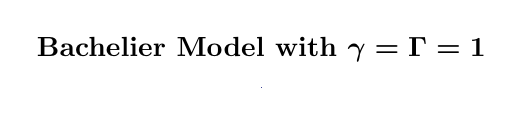
\begin{tikzpicture}[%
font=\footnotesize
]

\begin{axis}[%
width=0.951\figwidth,
height=\figheight,
at={(0\figwidth,0\figheight)},
scale only axis,
xmin=0,
xmax=3,
tick align=outside,
xlabel={$\bar P-p$},
xmajorgrids,
ymin=0,
ymax=1,
ylabel={$T-t$},
ymajorgrids,
zmin=0,
zmax=0.4,
zlabel={Relative Increase $\bar u_{\mathrm{BA}} / \bar u_{\mathrm{AC}}$},
zmajorgrids,
view={50}{40},
axis background/.style={fill=white},
title style={font=\bfseries},
title={Bachelier Model with $\boldsymbol{\gamma = \Gamma = 1}$},
axis x line*=bottom,
axis y line*=left,
axis z line*=left
]

\addplot3[%
surf,
shader=flat corner,draw=black,z buffer=sort,colormap={mymap}{[1pt] rgb(0pt)=(0.2081,0.1663,0.5292); rgb(1pt)=(0.211624,0.189781,0.577676); rgb(2pt)=(0.212252,0.213771,0.626971); rgb(3pt)=(0.2081,0.2386,0.677086); rgb(4pt)=(0.195905,0.264457,0.7279); rgb(5pt)=(0.170729,0.291938,0.779248); rgb(6pt)=(0.125271,0.324243,0.830271); rgb(7pt)=(0.0591333,0.359833,0.868333); rgb(8pt)=(0.0116952,0.38751,0.881957); rgb(9pt)=(0.00595714,0.408614,0.882843); rgb(10pt)=(0.0165143,0.4266,0.878633); rgb(11pt)=(0.0328524,0.443043,0.871957); rgb(12pt)=(0.0498143,0.458571,0.864057); rgb(13pt)=(0.0629333,0.47369,0.855438); rgb(14pt)=(0.0722667,0.488667,0.8467); rgb(15pt)=(0.0779429,0.503986,0.838371); rgb(16pt)=(0.0793476,0.520024,0.831181); rgb(17pt)=(0.0749429,0.537543,0.826271); rgb(18pt)=(0.0640571,0.556986,0.823957); rgb(19pt)=(0.0487714,0.577224,0.822829); rgb(20pt)=(0.0343429,0.596581,0.819852); rgb(21pt)=(0.0265,0.6137,0.8135); rgb(22pt)=(0.0238905,0.628662,0.803762); rgb(23pt)=(0.0230905,0.641786,0.791267); rgb(24pt)=(0.0227714,0.653486,0.776757); rgb(25pt)=(0.0266619,0.664195,0.760719); rgb(26pt)=(0.0383714,0.674271,0.743552); rgb(27pt)=(0.0589714,0.683757,0.725386); rgb(28pt)=(0.0843,0.692833,0.706167); rgb(29pt)=(0.113295,0.7015,0.685857); rgb(30pt)=(0.145271,0.709757,0.664629); rgb(31pt)=(0.180133,0.717657,0.642433); rgb(32pt)=(0.217829,0.725043,0.619262); rgb(33pt)=(0.258643,0.731714,0.595429); rgb(34pt)=(0.302171,0.737605,0.571186); rgb(35pt)=(0.348167,0.742433,0.547267); rgb(36pt)=(0.395257,0.7459,0.524443); rgb(37pt)=(0.44201,0.748081,0.503314); rgb(38pt)=(0.487124,0.749062,0.483976); rgb(39pt)=(0.530029,0.749114,0.466114); rgb(40pt)=(0.570857,0.748519,0.44939); rgb(41pt)=(0.609852,0.747314,0.433686); rgb(42pt)=(0.6473,0.7456,0.4188); rgb(43pt)=(0.683419,0.743476,0.404433); rgb(44pt)=(0.71841,0.741133,0.390476); rgb(45pt)=(0.752486,0.7384,0.376814); rgb(46pt)=(0.785843,0.735567,0.363271); rgb(47pt)=(0.818505,0.732733,0.34979); rgb(48pt)=(0.850657,0.7299,0.336029); rgb(49pt)=(0.882433,0.727433,0.3217); rgb(50pt)=(0.913933,0.725786,0.306276); rgb(51pt)=(0.944957,0.726114,0.288643); rgb(52pt)=(0.973895,0.731395,0.266648); rgb(53pt)=(0.993771,0.745457,0.240348); rgb(54pt)=(0.999043,0.765314,0.216414); rgb(55pt)=(0.995533,0.786057,0.196652); rgb(56pt)=(0.988,0.8066,0.179367); rgb(57pt)=(0.978857,0.827143,0.163314); rgb(58pt)=(0.9697,0.848138,0.147452); rgb(59pt)=(0.962586,0.870514,0.1309); rgb(60pt)=(0.958871,0.8949,0.113243); rgb(61pt)=(0.959824,0.921833,0.0948381); rgb(62pt)=(0.9661,0.951443,0.0755333); rgb(63pt)=(0.9763,0.9831,0.0538)},mesh/rows=25]
table[row sep=crcr, point meta=\thisrow{c}] {%
%
x	y	z	c\\
0	0.01	0.0210612144407193	0.0210612144407193\\
0	0.0302040816326531	0.0403346597539947	0.0403346597539947\\
0	0.0504081632653061	0.0565969805514202	0.0565969805514202\\
0	0.0706122448979592	0.0718888710486934	0.0718888710486934\\
0	0.0908163265306122	0.0866094135972352	0.0866094135972352\\
0	0.111020408163265	0.100846644884792	0.100846644884792\\
0	0.131224489795918	0.11459685753334	0.11459685753334\\
0	0.151428571428571	0.127828342042846	0.127828342042846\\
0	0.171632653061224	0.140504802977767	0.140504802977767\\
0	0.191836734693878	0.152594797045576	0.152594797045576\\
0	0.212040816326531	0.164075384703215	0.164075384703215\\
0	0.232244897959184	0.174933106797865	0.174933106797865\\
0	0.252448979591837	0.18516365645731	0.18516365645731\\
0	0.27265306122449	0.194770921376859	0.194770921376859\\
0	0.292857142857143	0.203765756839816	0.203765756839816\\
0	0.313061224489796	0.212164690842293	0.212164690842293\\
0	0.333265306122449	0.219988674855506	0.219988674855506\\
0	0.353469387755102	0.227261941860038	0.227261941860038\\
0	0.373673469387755	0.234011001347311	0.234011001347311\\
0	0.393877551020408	0.24026378104648	0.24026378104648\\
0	0.414081632653061	0.246048912850046	0.246048912850046\\
0	0.434285714285714	0.251395153177107	0.251395153177107\\
0	0.454489795918367	0.256330924156946	0.256330924156946\\
0	0.47469387755102	0.26088396039909	0.26088396039909\\
0	0.494897959183673	0.265081045955457	0.265081045955457\\
0	0.515102040816326	0.268947826818391	0.268947826818391\\
0	0.53530612244898	0.272508685548759	0.272508685548759\\
0	0.555510204081633	0.275786666129984	0.275786666129984\\
0	0.575714285714286	0.278803438711356	0.278803438711356\\
0	0.595918367346939	0.281579295441446	0.281579295441446\\
0	0.616122448979592	0.284133170008145	0.284133170008145\\
0	0.636326530612245	0.286482674793992	0.286482674793992\\
0	0.656530612244898	0.288644150671816	0.288644150671816\\
0	0.676734693877551	0.290632725444843	0.290632725444843\\
0	0.696938775510204	0.292462377752677	0.292462377752677\\
0	0.717142857142857	0.294146003956339	0.294146003956339\\
0	0.73734693877551	0.295695486083703	0.295695486083703\\
0	0.757551020408163	0.297121759383367	0.297121759383367\\
0	0.777755102040816	0.298434878410478	0.298434878410478\\
0	0.797959183673469	0.299644080872816	0.299644080872816\\
0	0.818163265306122	0.300757848702834	0.300757848702834\\
0	0.838367346938775	0.301783966011081	0.301783966011081\\
0	0.858571428571429	0.302729573722657	0.302729573722657\\
0	0.878775510204082	0.303601220808145	0.303601220808145\\
0	0.898979591836735	0.304404912109294	0.304404912109294\\
0	0.919183673469388	0.305146152814997	0.305146152814997\\
0	0.939387755102041	0.305829989696006	0.305829989696006\\
0	0.959591836734694	0.306461049229698	0.306461049229698\\
0	0.979795918367347	0.307043572773085	0.307043572773085\\
0	1	0.307581448949949	0.307581448949949\\
0.125	0.01	0.000100833503220867	0.000100833503220867\\
0.125	0.0302040816326531	0.00307327209442547	0.00307327209442547\\
0.125	0.0504081632653061	0.00828658823923841	0.00828658823923841\\
0.125	0.0706122448979592	0.0143634616298294	0.0143634616298294\\
0.125	0.0908163265306122	0.0208746112271512	0.0208746112271512\\
0.125	0.111020408163265	0.0276251744983474	0.0276251744983474\\
0.125	0.131224489795918	0.0344929369673377	0.0344929369673377\\
0.125	0.151428571428571	0.0413865985030929	0.0413865985030929\\
0.125	0.171632653061224	0.0482328703864381	0.0482328703864381\\
0.125	0.191836734693878	0.054971780162627	0.054971780162627\\
0.125	0.212040816326531	0.0615545428928234	0.0615545428928234\\
0.125	0.232244897959184	0.0679422490829336	0.0679422490829336\\
0.125	0.252448979591837	0.0741047962372138	0.0741047962372138\\
0.125	0.27265306122449	0.0800198847306534	0.0800198847306534\\
0.125	0.292857142857143	0.0856720367760695	0.0856720367760695\\
0.125	0.313061224489796	0.0910516439852945	0.0910516439852945\\
0.125	0.333265306122449	0.0961540613545291	0.0961540613545291\\
0.125	0.353469387755102	0.100978764937093	0.100978764937093\\
0.125	0.373673469387755	0.105528585614748	0.105528585614748\\
0.125	0.393877551020408	0.109809025777279	0.109809025777279\\
0.125	0.414081632653061	0.113827660766212	0.113827660766212\\
0.125	0.434285714285714	0.117593623087391	0.117593623087391\\
0.125	0.454489795918367	0.121117164658226	0.121117164658226\\
0.125	0.47469387755102	0.124409290869925	0.124409290869925\\
0.125	0.494897959183673	0.127481458569312	0.127481458569312\\
0.125	0.515102040816326	0.130345331161014	0.130345331161014\\
0.125	0.53530612244898	0.133012582680261	0.133012582680261\\
0.125	0.555510204081633	0.135494744004812	0.135494744004812\\
0.125	0.575714285714286	0.137803084646652	0.137803084646652\\
0.125	0.595918367346939	0.139948524271855	0.139948524271855\\
0.125	0.616122448979592	0.141941568787532	0.141941568787532\\
0.125	0.636326530612245	0.143792266511155	0.143792266511155\\
0.125	0.656530612244898	0.145510180742015	0.145510180742015\\
0.125	0.676734693877551	0.1471043746484	0.1471043746484\\
0.125	0.696938775510204	0.148583406777252	0.148583406777252\\
0.125	0.717142857142857	0.149955336443911	0.149955336443911\\
0.125	0.73734693877551	0.151227730629943	0.151227730629943\\
0.125	0.757551020408163	0.152407679675639	0.152407679675639\\
0.125	0.777755102040816	0.153501814272672	0.153501814272672\\
0.125	0.797959183673469	0.154516325048319	0.154516325048319\\
0.125	0.818163265306122	0.15545698358064	0.15545698358064\\
0.125	0.838367346938775	0.156329164206289	0.156329164206289\\
0.125	0.858571428571429	0.157137866122286	0.157137866122286\\
0.125	0.878775510204082	0.157887735397472	0.157887735397472\\
0.125	0.898979591836735	0.158583086602517	0.158583086602517\\
0.125	0.919183673469388	0.159227923842761	0.159227923842761\\
0.125	0.939387755102041	0.159825961038757	0.159825961038757\\
0.125	0.959591836734694	0.160380641347793	0.160380641347793\\
0.125	0.979795918367347	0.160895155657967	0.160895155657967\\
0.125	1	0.161372460116481	0.161372460116481\\
0.25	0.01	2.66214686692347e-09	2.66214686692347e-09\\
0.25	0.0302040816326531	5.13424295477615e-05	5.13424295477615e-05\\
0.25	0.0504081632653061	0.000524032140942082	0.000524032140942082\\
0.25	0.0706122448979592	0.00163326670119378	0.00163326670119378\\
0.25	0.0908163265306122	0.0033157322993156	0.0033157322993156\\
0.25	0.111020408163265	0.0054557933597366	0.0054557933597366\\
0.25	0.131224489795918	0.00794858310308109	0.00794858310308109\\
0.25	0.151428571428571	0.0107069780507524	0.0107069780507524\\
0.25	0.171632653061224	0.0136588495075286	0.0136588495075286\\
0.25	0.191836734693878	0.0167439072277735	0.0167439072277735\\
0.25	0.212040816326531	0.0199114194602945	0.0199114194602945\\
0.25	0.232244897959184	0.0231186603838352	0.0231186603838352\\
0.25	0.252448979591837	0.0263298069346422	0.0263298069346422\\
0.25	0.27265306122449	0.0295150891265303	0.0295150891265303\\
0.25	0.292857142857143	0.0326500805886868	0.0326500805886868\\
0.25	0.313061224489796	0.0357150705008004	0.0357150705008004\\
0.25	0.333265306122449	0.0386944894851271	0.0386944894851271\\
0.25	0.353469387755102	0.0415763785837355	0.0415763785837355\\
0.25	0.373673469387755	0.0443518983418142	0.0443518983418142\\
0.25	0.393877551020408	0.047014878129741	0.047014878129741\\
0.25	0.414081632653061	0.0495614064908705	0.0495614064908705\\
0.25	0.434285714285714	0.0519894628297633	0.0519894628297633\\
0.25	0.454489795918367	0.0542985898873186	0.0542985898873186\\
0.25	0.47469387755102	0.0564896055608063	0.0564896055608063\\
0.25	0.494897959183673	0.058564351889911	0.058564351889911\\
0.25	0.515102040816326	0.06052547850311	0.06052547850311\\
0.25	0.53530612244898	0.0623762575014149	0.0623762575014149\\
0.25	0.555510204081633	0.0641204266205316	0.0641204266205316\\
0.25	0.575714285714286	0.065762057519867	0.065762057519867\\
0.25	0.595918367346939	0.0673054461593121	0.0673054461593121\\
0.25	0.616122448979592	0.0687550224083897	0.0687550224083897\\
0.25	0.636326530612245	0.0701152762592683	0.0701152762592683\\
0.25	0.656530612244898	0.0713906982636158	0.0713906982636158\\
0.25	0.676734693877551	0.0725857320672704	0.0725857320672704\\
0.25	0.696938775510204	0.0737047371649948	0.0737047371649948\\
0.25	0.717142857142857	0.0747519602327329	0.0747519602327329\\
0.25	0.73734693877551	0.075731513612316	0.075731513612316\\
0.25	0.757551020408163	0.0766473597211854	0.0766473597211854\\
0.25	0.777755102040816	0.0775033003366446	0.0775033003366446\\
0.25	0.797959183673469	0.0783029698607659	0.0783029698607659\\
0.25	0.818163265306122	0.0790498318093482	0.0790498318093482\\
0.25	0.838367346938775	0.0797471778876735	0.0797471778876735\\
0.25	0.858571428571429	0.0803981291188782	0.0803981291188782\\
0.25	0.878775510204082	0.0810056385792172	0.0810056385792172\\
0.25	0.898979591836735	0.0815724953700522	0.0815724953700522\\
0.25	0.919183673469388	0.0821013295206123	0.0821013295206123\\
0.25	0.939387755102041	0.0825946175699415	0.0825946175699415\\
0.25	0.959591836734694	0.0830546886222918	0.0830546886222918\\
0.25	0.979795918367347	0.08348373070875	0.08348373070875\\
0.25	1	0.0838837973201518	0.0838837973201518\\
0.375	0.01	2.04267651458558e-16	2.04267651458558e-16\\
0.375	0.0302040816326531	1.45016357217975e-07	1.45016357217975e-07\\
0.375	0.0504081632653061	1.21910221112651e-05	1.21910221112651e-05\\
0.375	0.0706122448979592	9.43843203100581e-05	9.43843203100581e-05\\
0.375	0.0908163265306122	0.000318710065918877	0.000318710065918877\\
0.375	0.111020408163265	0.000726441281252369	0.000726441281252369\\
0.375	0.131224489795918	0.00132821393279266	0.00132821393279266\\
0.375	0.151428571428571	0.00211589065790456	0.00211589065790456\\
0.375	0.171632653061224	0.00307163125259468	0.00307163125259468\\
0.375	0.191836734693878	0.00417325081067671	0.00417325081067671\\
0.375	0.212040816326531	0.00539720184025024	0.00539720184025024\\
0.375	0.232244897959184	0.00672022510924219	0.00672022510924219\\
0.375	0.252448979591837	0.00812026563933737	0.00812026563933737\\
0.375	0.27265306122449	0.00957697075308162	0.00957697075308162\\
0.375	0.292857142857143	0.0110719389075085	0.0110719389075085\\
0.375	0.313061224489796	0.012588812823175	0.012588812823175\\
0.375	0.333265306122449	0.0141132720867962	0.0141132720867962\\
0.375	0.353469387755102	0.0156329601783916	0.0156329601783916\\
0.375	0.373673469387755	0.0171373695107939	0.0171373695107939\\
0.375	0.393877551020408	0.0186177011342061	0.0186177011342061\\
0.375	0.414081632653061	0.0200667111408703	0.0200667111408703\\
0.375	0.434285714285714	0.0214785524992874	0.0214785524992874\\
0.375	0.454489795918367	0.0228486185656081	0.0228486185656081\\
0.375	0.47469387755102	0.0241733926125011	0.0241733926125011\\
0.375	0.494897959183673	0.0254503062428029	0.0254503062428029\\
0.375	0.515102040816326	0.0266776084263474	0.0266776084263474\\
0.375	0.53530612244898	0.0278542460472217	0.0278542460472217\\
0.375	0.555510204081633	0.0289797562218911	0.0289797562218911\\
0.375	0.575714285714286	0.0300541702012944	0.0300541702012944\\
0.375	0.595918367346939	0.0310779283640688	0.0310779283640688\\
0.375	0.616122448979592	0.0320518056114751	0.0320518056114751\\
0.375	0.636326530612245	0.0329768463608335	0.0329768463608335\\
0.375	0.656530612244898	0.0338543082817311	0.0338543082817311\\
0.375	0.676734693877551	0.0346856139107061	0.0346856139107061\\
0.375	0.696938775510204	0.0354723093020358	0.0354723093020358\\
0.375	0.717142857142857	0.0362160289142928	0.0362160289142928\\
0.375	0.73734693877551	0.0369184659866781	0.0369184659866781\\
0.375	0.757551020408163	0.0375813477200405	0.0375813477200405\\
0.375	0.777755102040816	0.0382064146408181	0.0382064146408181\\
0.375	0.797959183673469	0.0387954035890175	0.0387954035890175\\
0.375	0.818163265306122	0.0393500338318488	0.0393500338318488\\
0.375	0.838367346938775	0.0398719958615528	0.0398719958615528\\
0.375	0.858571428571429	0.0403629424885983	0.0403629424885983\\
0.375	0.878775510204082	0.0408244818894763	0.0408244818894763\\
0.375	0.898979591836735	0.0412581723117094	0.0412581723117094\\
0.375	0.919183673469388	0.0416655181775646	0.0416655181775646\\
0.375	0.939387755102041	0.0420479673625161	0.0420479673625161\\
0.375	0.959591836734694	0.0424069094550687	0.0424069094550687\\
0.375	0.979795918367347	0.0427436748314399	0.0427436748314399\\
0.375	1	0.0430595344021635	0.0430595344021635\\
0.5	0.01	3.70536611252091e-26	3.70536611252091e-26\\
0.5	0.0302040816326531	6.11662700410701e-11	6.11662700410701e-11\\
0.5	0.0504081632653061	9.52524053177045e-08	9.52524053177045e-08\\
0.5	0.0706122448979592	2.57959954473353e-06	2.57959954473353e-06\\
0.5	0.0908163265306122	1.7477288454993e-05	1.7477288454993e-05\\
0.5	0.111020408163265	6.20708063247399e-05	6.20708063247399e-05\\
0.5	0.131224489795918	0.000154313711764388	0.000154313711764388\\
0.5	0.151428571428571	0.000308026302207943	0.000308026302207943\\
0.5	0.171632653061224	0.000531458291396787	0.000531458291396787\\
0.5	0.191836734693878	0.00082772801782941	0.00082772801782941\\
0.5	0.212040816326531	0.00119589806566513	0.00119589806566513\\
0.5	0.232244897959184	0.00163210023543333	0.00163210023543333\\
0.5	0.252448979591837	0.00213050307121952	0.00213050307121952\\
0.5	0.27265306122449	0.00268407920742498	0.00268407920742498\\
0.5	0.292857142857143	0.00328518835827157	0.00328518835827157\\
0.5	0.313061224489796	0.00392600726555501	0.00392600726555501\\
0.5	0.333265306122449	0.00459883800870979	0.00459883800870979\\
0.5	0.353469387755102	0.00529632167061572	0.00529632167061572\\
0.5	0.373673469387755	0.006011579325872	0.006011579325872\\
0.5	0.393877551020408	0.00673829785523171	0.00673829785523171\\
0.5	0.414081632653061	0.00747077441531196	0.00747077441531196\\
0.5	0.434285714285714	0.00820393043869454	0.00820393043869454\\
0.5	0.454489795918367	0.00893330367723175	0.00893330367723175\\
0.5	0.47469387755102	0.00965502491128379	0.00965502491128379\\
0.5	0.494897959183673	0.0103657844341751	0.0103657844341751\\
0.5	0.515102040816326	0.0110627922105924	0.0110627922105924\\
0.5	0.53530612244898	0.0117437346426325	0.0117437346426325\\
0.5	0.555510204081633	0.012406730112233	0.012406730112233\\
0.5	0.575714285714286	0.0130502848668603	0.0130502848668603\\
0.5	0.595918367346939	0.0136732503461369	0.0136732503461369\\
0.5	0.616122448979592	0.0142747826852707	0.0142747826852707\\
0.5	0.636326530612245	0.0148543048556182	0.0148543048556182\\
0.5	0.656530612244898	0.0154114716960058	0.0154114716960058\\
0.5	0.676734693877551	0.0159461379360971	0.0159461379360971\\
0.5	0.696938775510204	0.0164583292033332	0.0164583292033332\\
0.5	0.717142857142857	0.0169482159281889	0.0169482159281889\\
0.5	0.73734693877551	0.0174160900109619	0.0174160900109619\\
0.5	0.757551020408163	0.0178623440808989	0.0178623440808989\\
0.5	0.777755102040816	0.0182874531602906	0.0182874531602906\\
0.5	0.797959183673469	0.0186919585384416	0.0186919585384416\\
0.5	0.818163265306122	0.0190764536601752	0.0190764536601752\\
0.5	0.838367346938775	0.0194415718385189	0.0194415718385189\\
0.5	0.858571428571429	0.0197879756096901	0.0197879756096901\\
0.5	0.878775510204082	0.0201163475591919	0.0201163475591919\\
0.5	0.898979591836735	0.0204273824597604	0.0204273824597604\\
0.5	0.919183673469388	0.0207217805743898	0.0207217805743898\\
0.5	0.939387755102041	0.021000241990203	0.021000241990203\\
0.5	0.959591836734694	0.0212634618611759	0.0212634618611759\\
0.5	0.979795918367347	0.0215121264494469	0.0215121264494469\\
0.5	1	0.0217469098659954	0.0217469098659954\\
0.625	0.01	1.46096456877253e-38	1.46096456877253e-38\\
0.625	0.0302040816326531	3.62048995378054e-15	3.62048995378054e-15\\
0.625	0.0504081632653061	2.37521442257473e-10	2.37521442257473e-10\\
0.625	0.0706122448979592	3.19154656134518e-08	3.19154656134518e-08\\
0.625	0.0908163265306122	5.26209736279742e-07	5.26209736279742e-07\\
0.625	0.111020408163265	3.28975445364692e-06	3.28975445364692e-06\\
0.625	0.131224489795918	1.20929864172203e-05	1.20929864172203e-05\\
0.625	0.151428571428571	3.21468555898644e-05	3.21468555898644e-05\\
0.625	0.171632653061224	6.903427741094e-05	6.903427741094e-05\\
0.625	0.191836734693878	0.000127776039526654	0.000127776039526654\\
0.625	0.212040816326531	0.000212275048035443	0.000212275048035443\\
0.625	0.232244897959184	0.000325104553562668	0.000325104553562668\\
0.625	0.252448979591837	0.000467526949281466	0.000467526949281466\\
0.625	0.27265306122449	0.00063963982893074	0.00063963982893074\\
0.625	0.292857142857143	0.000840577452386052	0.000840577452386052\\
0.625	0.313061224489796	0.00106872393657351	0.00106872393657351\\
0.625	0.333265306122449	0.00132191425033003	0.00132191425033003\\
0.625	0.353469387755102	0.00159761153950485	0.00159761153950485\\
0.625	0.373673469387755	0.00189305665405592	0.00189305665405592\\
0.625	0.393877551020408	0.00220538984507747	0.00220538984507747\\
0.625	0.414081632653061	0.00253174672184351	0.00253174672184351\\
0.625	0.434285714285714	0.00286933151765521	0.00286933151765521\\
0.625	0.454489795918367	0.00321547100527225	0.00321547100527225\\
0.625	0.47469387755102	0.00356765232710627	0.00356765232710627\\
0.625	0.494897959183673	0.00392354774049354	0.00392354774049354\\
0.625	0.515102040816326	0.00428102892949806	0.00428102892949806\\
0.625	0.53530612244898	0.00463817316288255	0.00463817316288255\\
0.625	0.555510204081633	0.00499326321736341	0.00499326321736341\\
0.625	0.575714285714286	0.00534478265398632	0.00534478265398632\\
0.625	0.595918367346939	0.00569140774151245	0.00569140774151245\\
0.625	0.616122448979592	0.0060319970663143	0.0060319970663143\\
0.625	0.636326530612245	0.00636557965228029	0.00636557965228029\\
0.625	0.656530612244898	0.00669134223363409	0.00669134223363409\\
0.625	0.676734693877551	0.00700861617454851	0.00700861617454851\\
0.625	0.696938775510204	0.00731686440787937	0.00731686440787937\\
0.625	0.717142857142857	0.00761566866726211	0.00761566866726211\\
0.625	0.73734693877551	0.00790471720849159	0.00790471720849159\\
0.625	0.757551020408163	0.00818379315421994	0.00818379315421994\\
0.625	0.777755102040816	0.00845276354764963	0.00845276354764963\\
0.625	0.797959183673469	0.00871156916357363	0.00871156916357363\\
0.625	0.818163265306122	0.00896021509671039	0.00896021509671039\\
0.625	0.838367346938775	0.00919876212603186	0.00919876212603186\\
0.625	0.858571428571429	0.00942731883822779	0.00942731883822779\\
0.625	0.878775510204082	0.00964603448238856	0.00964603448238856\\
0.625	0.898979591836735	0.00985509252044535	0.00985509252044535\\
0.625	0.919183673469388	0.0100547048330902	0.0100547048330902\\
0.625	0.939387755102041	0.0102451065381732	0.0102451065381732\\
0.625	0.959591836734694	0.0104265513774342	0.0104265513774342\\
0.625	0.979795918367347	0.0105993076274628	0.0105993076274628\\
0.625	1	0.0107636544916877	0.0107636544916877\\
0.75	0.01	1.20144152682882e-53	1.20144152682882e-53\\
0.75	0.0302040816326531	2.90681293685828e-20	2.90681293685828e-20\\
0.75	0.0504081632653061	1.83467064698255e-13	1.83467064698255e-13\\
0.75	0.0706122448979592	1.73987448226889e-10	1.73987448226889e-10\\
0.75	0.0908163265306122	8.48568547889218e-09	8.48568547889218e-09\\
0.75	0.111020408163265	1.05703030602842e-07	1.05703030602842e-07\\
0.75	0.131224489795918	6.25815194960543e-07	6.25815194960543e-07\\
0.75	0.151428571428571	2.35831523615301e-06	2.35831523615301e-06\\
0.75	0.171632653061224	6.61030206761237e-06	6.61030206761237e-06\\
0.75	0.191836734693878	1.50932290785037e-05	1.50932290785037e-05\\
0.75	0.212040816326531	2.97107330396199e-05	2.97107330396199e-05\\
0.75	0.232244897959184	5.23364793770872e-05	5.23364793770872e-05\\
0.75	0.252448979591837	8.46357409323836e-05	8.46357409323836e-05\\
0.75	0.27265306122449	0.000127948831021385	0.000127948831021385\\
0.75	0.292857142857143	0.000183233068109953	0.000183233068109953\\
0.75	0.313061224489796	0.000251050933304342	0.000251050933304342\\
0.75	0.333265306122449	0.000331590402579022	0.000331590402579022\\
0.75	0.353469387755102	0.000424705119942457	0.000424705119942457\\
0.75	0.373673469387755	0.000529964834947202	0.000529964834947202\\
0.75	0.393877551020408	0.000646709263762427	0.000646709263762427\\
0.75	0.414081632653061	0.000774100827079549	0.000774100827079549\\
0.75	0.434285714285714	0.000911173478832662	0.000911173478832662\\
0.75	0.454489795918367	0.00105687611387886	0.00105687611387886\\
0.75	0.47469387755102	0.00121010992171189	0.00121010992171189\\
0.75	0.494897959183673	0.00136975963121529	0.00136975963121529\\
0.75	0.515102040816326	0.00153471894985004	0.00153471894985004\\
0.75	0.53530612244898	0.00170391070429255	0.00170391070429255\\
0.75	0.555510204081633	0.00187630228747626	0.00187630228747626\\
0.75	0.575714285714286	0.00205091704524045	0.00205091704524045\\
0.75	0.595918367346939	0.00222684222008909	0.00222684222008909\\
0.75	0.616122448979592	0.00240323402789671	0.00240323402789671\\
0.75	0.636326530612245	0.00257932038804216	0.00257932038804216\\
0.75	0.656530612244898	0.0027544017665596	0.0027544017665596\\
0.75	0.676734693877551	0.00292785053069772	0.00292785053069772\\
0.75	0.696938775510204	0.00309910915495902	0.00309910915495902\\
0.75	0.717142857142857	0.00326768756504235	0.00326768756504235\\
0.75	0.73734693877551	0.00343315985798724	0.00343315985798724\\
0.75	0.757551020408163	0.00359516059446285	0.00359516059446285\\
0.75	0.777755102040816	0.00375338082242377	0.00375338082242377\\
0.75	0.797959183673469	0.00390756395991087	0.00390756395991087\\
0.75	0.818163265306122	0.00405750163813222	0.00405750163813222\\
0.75	0.838367346938775	0.00420302958359461	0.00420302958359461\\
0.75	0.858571428571429	0.00434402359944299	0.00434402359944299\\
0.75	0.878775510204082	0.00448039569080104	0.00448039569080104\\
0.75	0.898979591836735	0.00461209036632715	0.00461209036632715\\
0.75	0.919183673469388	0.00473908113798734	0.00473908113798734\\
0.75	0.939387755102041	0.00486136723283071	0.00486136723283071\\
0.75	0.959591836734694	0.0049789705240093	0.0049789705240093\\
0.75	0.979795918367347	0.00509193268313452	0.00509193268313452\\
0.75	1	0.00520031255206551	0.00520031255206551\\
0.875	0.01	2.01370079391801e-71	2.01370079391801e-71\\
0.875	0.0302040816326531	3.10234180389604e-26	3.10234180389604e-26\\
0.875	0.0504081632653061	4.30950505600495e-17	4.30950505600495e-17\\
0.875	0.0706122448979592	4.10778490497631e-13	4.10778490497631e-13\\
0.875	0.0908163265306122	7.21054635878971e-11	7.21054635878971e-11\\
0.875	0.111020408163265	2.02730328609521e-09	2.02730328609521e-09\\
0.875	0.131224489795918	2.10728878232124e-08	2.10728878232124e-08\\
0.875	0.151428571428571	1.19913311104581e-07	1.19913311104581e-07\\
0.875	0.171632653061224	4.60389280996198e-07	4.60389280996198e-07\\
0.875	0.191836734693878	1.34697335148329e-06	1.34697335148329e-06\\
0.875	0.212040816326531	3.2395587857969e-06	3.2395587857969e-06\\
0.875	0.232244897959184	6.73134918223265e-06	6.73134918223265e-06\\
0.875	0.252448979591837	1.25020988151483e-05	1.25020988151483e-05\\
0.875	0.27265306122449	2.12613321542983e-05	2.12613321542983e-05\\
0.875	0.292857142857143	3.36937382839652e-05	3.36937382839652e-05\\
0.875	0.313061224489796	5.04142100469044e-05	5.04142100469044e-05\\
0.875	0.333265306122449	7.19356592931022e-05	7.19356592931022e-05\\
0.875	0.353469387755102	9.86497203384543e-05	9.86497203384543e-05\\
0.875	0.373673469387755	0.000130818748577003	0.000130818748577003\\
0.875	0.393877551020408	0.000168576795821855	0.000168576795821855\\
0.875	0.414081632653061	0.000211937136318042	0.000211937136318042\\
0.875	0.434285714285714	0.000260804144189372	0.000260804144189372\\
0.875	0.454489795918367	0.000314987694839155	0.000314987694839155\\
0.875	0.47469387755102	0.000374218666362015	0.000374218666362015\\
0.875	0.494897959183673	0.000438164492272487	0.000438164492272487\\
0.875	0.515102040816326	0.000506444037191888	0.000506444037191888\\
0.875	0.53530612244898	0.000578641325319799	0.000578641325319799\\
0.875	0.555510204081633	0.000654317850533481	0.000654317850533481\\
0.875	0.575714285714286	0.000733023344433923	0.000733023344433923\\
0.875	0.595918367346939	0.000814304983676315	0.000814304983676315\\
0.875	0.616122448979592	0.000897715089349172	0.000897715089349172\\
0.875	0.636326530612245	0.000982817416859877	0.000982817416859877\\
0.875	0.656530612244898	0.0010691921613264	0.0010691921613264\\
0.875	0.676734693877551	0.00115643981616525	0.00115643981616525\\
0.875	0.696938775510204	0.00124418402554761	0.00124418402554761\\
0.875	0.717142857142857	0.00133207356783002	0.00133207356783002\\
0.875	0.73734693877551	0.00141978359931252	0.00141978359931252\\
0.875	0.757551020408163	0.00150701627745993	0.00150701627745993\\
0.875	0.777755102040816	0.00159350087127097	0.00159350087127097\\
0.875	0.797959183673469	0.00167899345465317	0.00167899345465317\\
0.875	0.818163265306122	0.00176327626703329	0.00176327626703329\\
0.875	0.838367346938775	0.00184615681437393	0.00184615681437393\\
0.875	0.858571428571429	0.00192746677349833	0.00192746677349833\\
0.875	0.878775510204082	0.00200706075326115	0.00200706075326115\\
0.875	0.898979591836735	0.00208481495768642	0.00208481495768642\\
0.875	0.919183673469388	0.00216062578871633	0.00216062578871633\\
0.875	0.939387755102041	0.00223440841963828	0.00223440841963828\\
0.875	0.959591836734694	0.00230609536452282	0.00230609536452282\\
0.875	0.979795918367347	0.00237563506404397	0.00237563506404397\\
0.875	1	0.00244299050379228	0.00244299050379228\\
1	0.01	6.78220443089767e-92	6.78220443089767e-92\\
1	0.0302040816326531	4.34518749116876e-33	4.34518749116876e-33\\
1	0.0504081632653061	3.04149767071536e-21	3.04149767071536e-21\\
1	0.0706122448979592	4.1522602210983e-16	4.1522602210983e-16\\
1	0.0908163265306122	3.19296170198942e-13	3.19296170198942e-13\\
1	0.111020408163265	2.29613196951882e-11	2.29613196951882e-11\\
1	0.131224489795918	4.56923969989326e-10	4.56923969989326e-10\\
1	0.151428571428571	4.18356026071275e-09	4.18356026071275e-09\\
1	0.171632653061224	2.30952635407958e-08	2.30952635407958e-08\\
1	0.191836734693878	8.99630070006988e-08	8.99630070006988e-08\\
1	0.212040816326531	2.72671329207557e-07	2.72671329207557e-07\\
1	0.232244897959184	6.85611477925605e-07	6.85611477925605e-07\\
1	0.252448979591837	1.49414925837989e-06	1.49414925837989e-06\\
1	0.27265306122449	2.91093726825493e-06	2.91093726825493e-06\\
1	0.292857142857143	5.18536741109287e-06	5.18536741109287e-06\\
1	0.313061224489796	8.58876008607387e-06	8.58876008607387e-06\\
1	0.333265306122449	1.33980519286866e-05	1.33980519286866e-05\\
1	0.353469387755102	1.98802349998902e-05	1.98802349998902e-05\\
1	0.373673469387755	2.82790485055447e-05	2.82790485055447e-05\\
1	0.393877551020408	3.88047020227259e-05	3.88047020227259e-05\\
1	0.414081632653061	5.16268412279519e-05	5.16268412279519e-05\\
1	0.434285714285714	6.68705813648655e-05	6.68705813648655e-05\\
1	0.454489795918367	8.46152094080895e-05	8.46152094080895e-05\\
1	0.47469387755102	0.000104895054771198	0.000104895054771198\\
1	0.494897959183673	0.000127702011415767	0.000127702011415767\\
1	0.515102040816326	0.000152989228747583	0.000152989228747583\\
1	0.53530612244898	0.000180675550461837	0.000180675550461837\\
1	0.555510204081633	0.000210650352929417	0.000210650352929417\\
1	0.575714285714286	0.000242778507343516	0.000242778507343516\\
1	0.595918367346939	0.000276905256695981	0.000276905256695981\\
1	0.616122448979592	0.000312860856814909	0.000312860856814909\\
1	0.636326530612245	0.000350464879221984	0.000350464879221984\\
1	0.656530612244898	0.000389530112685914	0.000389530112685914\\
1	0.676734693877551	0.00042986603091627	0.00042986603091627\\
1	0.696938775510204	0.000471281817002246	0.000471281817002246\\
1	0.717142857142857	0.000513588952163625	0.000513588952163625\\
1	0.73734693877551	0.000556603388301624	0.000556603388301624\\
1	0.757551020408163	0.000600147331752682	0.000600147331752682\\
1	0.777755102040816	0.000644050670452438	0.000644050670452438\\
1	0.797959183673469	0.000688152079158269	0.000688152079158269\\
1	0.818163265306122	0.000732299838067798	0.000732299838067798\\
1	0.838367346938775	0.000776352399597823	0.000776352399597823\\
1	0.858571428571429	0.000820178736638858	0.000820178736638858\\
1	0.878775510204082	0.000863658503573949	0.000863658503573949\\
1	0.898979591836735	0.000906682038974639	0.000906682038974639\\
1	0.919183673469388	0.000949150236332422	0.000949150236332422\\
1	0.939387755102041	0.000990974306576141	0.000990974306576141\\
1	0.959591836734694	0.00103207545355404	0.00103207545355404\\
1	0.979795918367347	0.00107238448118565	0.00107238448118565\\
1	1	0.00111184134865422	0.00111184134865422\\
1.125	0.01	4.54779037811358e-115	4.54779037811358e-115\\
1.125	0.0302040816326531	7.91826621608916e-41	7.91826621608916e-41\\
1.125	0.0504081632653061	6.39697983421135e-26	6.39697983421135e-26\\
1.125	0.0706122448979592	1.78279786617457e-19	1.78279786617457e-19\\
1.125	0.0908163265306122	7.3113621529174e-16	7.3113621529174e-16\\
1.125	0.111020408163265	1.52412064842215e-13	1.52412064842215e-13\\
1.125	0.131224489795918	6.33225715336292e-12	6.33225715336292e-12\\
1.125	0.151428571428571	9.94133334794872e-11	9.94133334794872e-11\\
1.125	0.171632653061224	8.28471840135013e-10	8.28471840135013e-10\\
1.125	0.191836734693878	4.46499084213919e-09	4.46499084213919e-09\\
1.125	0.212040816326531	1.75938987460922e-08	1.75938987460922e-08\\
1.125	0.232244897959184	5.49273082145259e-08	5.49273082145259e-08\\
1.125	0.252448979591837	1.43520452152906e-07	1.43520452152906e-07\\
1.125	0.27265306122449	3.26259387546772e-07	3.26259387546772e-07\\
1.125	0.292857142857143	6.63694197400803e-07	6.63694197400803e-07\\
1.125	0.313061224489796	1.2337892818823e-06	1.2337892818823e-06\\
1.125	0.333265306122449	2.12967536460595e-06	2.12967536460595e-06\\
1.125	0.353469387755102	3.45584708635271e-06	3.45584708635271e-06\\
1.125	0.373673469387755	5.32341338275689e-06	5.32341338275689e-06\\
1.125	0.393877551020408	7.84501041822796e-06	7.84501041822796e-06\\
1.125	0.414081632653061	1.11298898403139e-05	1.11298898403139e-05\\
1.125	0.434285714285714	1.52795548670999e-05	1.52795548670999e-05\\
1.125	0.454489795918367	2.03841729678003e-05	2.03841729678003e-05\\
1.125	0.47469387755102	2.65198692066255e-05	2.65198692066255e-05\\
1.125	0.494897959183673	3.37469080699973e-05	3.37469080699973e-05\\
1.125	0.515102040816326	4.21087047493747e-05	4.21087047493747e-05\\
1.125	0.53530612244898	5.16315658804578e-05	5.16315658804578e-05\\
1.125	0.555510204081633	6.2325039324453e-05	6.2325039324453e-05\\
1.125	0.575714285714286	7.41827472099277e-05	7.41827472099277e-05\\
1.125	0.595918367346939	8.71835812546968e-05	8.71835812546968e-05\\
1.125	0.616122448979592	0.000101293150420186	0.000101293150420186\\
1.125	0.636326530612245	0.000116465385254041	0.000116465385254041\\
1.125	0.656530612244898	0.000132644218753415	0.000132644218753415\\
1.125	0.676734693877551	0.000149765278837572	0.000149765278837572\\
1.125	0.696938775510204	0.000167757541698055	0.000167757541698055\\
1.125	0.717142857142857	0.000186544907932079	0.000186544907932079\\
1.125	0.73734693877551	0.000206047674265195	0.000206047674265195\\
1.125	0.757551020408163	0.000226183882815919	0.000226183882815919\\
1.125	0.777755102040816	0.000246870537341021	0.000246870537341021\\
1.125	0.797959183673469	0.000268024681879977	0.000268024681879977\\
1.125	0.818163265306122	0.000289564341873288	0.000289564341873288\\
1.125	0.838367346938775	0.000311409331351162	0.000311409331351162\\
1.125	0.858571428571429	0.00033348193235865	0.00033348193235865\\
1.125	0.878775510204082	0.000355707454568463	0.000355707454568463\\
1.125	0.898979591836735	0.000378014684182797	0.000378014684182797\\
1.125	0.919183673469388	0.000400336231870526	0.000400336231870526\\
1.125	0.939387755102041	0.000422608789736898	0.000422608789736898\\
1.125	0.959591836734694	0.000444773307272466	0.000444773307272466\\
1.125	0.979795918367347	0.000466775095953326	0.000466775095953326\\
1.125	1	0.000488563871728732	0.000488563871728732\\
1.25	0.01	6.03256166089891e-141	6.03256166089891e-141\\
1.25	0.0302040816326531	1.86607302570566e-49	1.86607302570566e-49\\
1.25	0.0504081632653061	3.98623613205909e-31	3.98623613205909e-31\\
1.25	0.0706122448979592	3.23292260641343e-23	3.23292260641343e-23\\
1.25	0.0908163265306122	8.60906258010331e-19	8.60906258010331e-19\\
1.25	0.111020408163265	5.89638881155552e-16	5.89638881155552e-16\\
1.25	0.131224489795918	5.57811554217882e-14	5.57811554217882e-14\\
1.25	0.151428571428571	1.60029829294735e-12	1.60029829294735e-12\\
1.25	0.171632653061224	2.1137160494968e-11	2.1137160494968e-11\\
1.25	0.191836734693878	1.63797694080054e-10	1.63797694080054e-10\\
1.25	0.212040816326531	8.6568157279197e-10	8.6568157279197e-10\\
1.25	0.232244897959184	3.44323365958778e-09	3.44323365958778e-09\\
1.25	0.252448979591837	1.10232249921507e-08	1.10232249921507e-08\\
1.25	0.27265306122449	2.97839940055839e-08	2.97839940055839e-08\\
1.25	0.292857142857143	7.02998914939369e-08	7.02998914939369e-08\\
1.25	0.313061224489796	1.48718276124705e-07	1.48718276124705e-07\\
1.25	0.333265306122449	2.87528071429852e-07	2.87528071429852e-07\\
1.25	0.353469387755102	5.15771286944168e-07	5.15771286944168e-07\\
1.25	0.373673469387755	8.68660416233566e-07	8.68660416233566e-07\\
1.25	0.393877551020408	1.38666094349117e-06	1.38666094349117e-06\\
1.25	0.414081632653061	2.11416216046157e-06	2.11416216046157e-06\\
1.25	0.434285714285714	3.09788864207247e-06	3.09788864207247e-06\\
1.25	0.454489795918367	4.38520525006764e-06	4.38520525006764e-06\\
1.25	0.47469387755102	6.02244983526433e-06	6.02244983526433e-06\\
1.25	0.494897959183673	8.05339898890913e-06	8.05339898890913e-06\\
1.25	0.515102040816326	1.0517940382475e-05	1.0517940382475e-05\\
1.25	0.53530612244898	1.34509951965031e-05	1.34509951965031e-05\\
1.25	0.555510204081633	1.68817085373334e-05	1.68817085373334e-05\\
1.25	0.575714285714286	2.08329056610081e-05	2.08329056610081e-05\\
1.25	0.595918367346939	2.53207973060705e-05	2.53207973060705e-05\\
1.25	0.616122448979592	3.03549079182046e-05	3.03549079182046e-05\\
1.25	0.636326530612245	3.59381951854314e-05	3.59381951854314e-05\\
1.25	0.656530612244898	4.20673271787326e-05	4.20673271787326e-05\\
1.25	0.676734693877551	4.87330836493554e-05	4.87330836493554e-05\\
1.25	0.696938775510204	5.59208499265681e-05	5.59208499265681e-05\\
1.25	0.717142857142857	6.36111747822876e-05	6.36111747822876e-05\\
1.25	0.73734693877551	7.17803671119938e-05	7.17803671119938e-05\\
1.25	0.757551020408163	8.04011099768077e-05	8.04011099768077e-05\\
1.25	0.777755102040816	8.94430742140422e-05	8.94430742140422e-05\\
1.25	0.797959183673469	9.88735172895021e-05	9.88735172895021e-05\\
1.25	0.818163265306122	0.000108657856234117	0.000108657856234117\\
1.25	0.838367346938775	0.000118760206326974	0.000118760206326974\\
1.25	0.858571428571429	0.000129143879637033	0.000129143879637033\\
1.25	0.878775510204082	0.000139771839620554	0.000139771839620554\\
1.25	0.898979591836735	0.000150607109709403	0.000150607109709403\\
1.25	0.919183673469388	0.00016161313524496	0.00016161313524496\\
1.25	0.939387755102041	0.000172754099246192	0.000172754099246192\\
1.25	0.959591836734694	0.000183995193382906	0.000183995193382906\\
1.25	0.979795918367347	0.000195302846190543	0.000195302846190543\\
1.25	1	0.000206644911043437	0.000206644911043437\\
1.375	0.01	1.57570726682024e-169	1.57570726682024e-169\\
1.375	0.0302040816326531	5.66233440948919e-59	5.66233440948919e-59\\
1.375	0.0504081632653061	7.32825620986719e-37	7.32825620986719e-37\\
1.375	0.0706122448979592	2.46574371297682e-27	2.46574371297682e-27\\
1.375	0.0908163265306122	5.19122251476901e-22	5.19122251476901e-22\\
1.375	0.111020408163265	1.32406815996878e-18	1.32406815996878e-18\\
1.375	0.131224489795918	3.11063291165556e-16	3.11063291165556e-16\\
1.375	0.151428571428571	1.73794276529318e-14	1.73794276529318e-14\\
1.375	0.171632653061224	3.81990641446677e-13	3.81990641446677e-13\\
1.375	0.191836734693878	4.42336453181615e-12	4.42336453181615e-12\\
1.375	0.212040816326531	3.23490219355222e-11	3.23490219355222e-11\\
1.375	0.232244897959184	1.68211248716505e-10	1.68211248716505e-10\\
1.375	0.252448979591837	6.74268473857266e-10	6.74268473857266e-10\\
1.375	0.27265306122449	2.20577588781964e-09	2.20577588781964e-09\\
1.375	0.292857142857143	6.137976806538e-09	6.137976806538e-09\\
1.375	0.313061224489796	1.49832319559705e-08	1.49832319559705e-08\\
1.375	0.333265306122449	3.2844913252055e-08	3.2844913252055e-08\\
1.375	0.353469387755102	6.5838162172865e-08	6.5838162172865e-08\\
1.375	0.373673469387755	1.22409714182571e-07	1.22409714182571e-07\\
1.375	0.393877551020408	2.13506031357417e-07	2.13506031357417e-07\\
1.375	0.414081632653061	3.525637090926e-07	3.525637090926e-07\\
1.375	0.434285714285714	5.55321403986396e-07	5.55321403986396e-07\\
1.375	0.454489795918367	8.39473395348674e-07	8.39473395348674e-07\\
1.375	0.47469387755102	1.22419896016391e-06	1.22419896016391e-06\\
1.375	0.494897959183673	1.7296087345623e-06	1.7296087345623e-06\\
1.375	0.515102040816326	2.37615018995236e-06	2.37615018995236e-06\\
1.375	0.53530612244898	3.18401088737844e-06	3.18401088737844e-06\\
1.375	0.555510204081633	4.17255197255782e-06	4.17255197255782e-06\\
1.375	0.575714285714286	5.35979688966638e-06	5.35979688966638e-06\\
1.375	0.595918367346939	6.76199262639082e-06	6.76199262639082e-06\\
1.375	0.616122448979592	8.39325369720662e-06	8.39325369720662e-06\\
1.375	0.636326530612245	1.02652929555071e-05	1.02652929555071e-05\\
1.375	0.656530612244898	1.23872383868126e-05	1.23872383868126e-05\\
1.375	0.676734693877551	1.47655312951017e-05	1.47655312951017e-05\\
1.375	0.696938775510204	1.74038986661167e-05	1.74038986661167e-05\\
1.375	0.717142857142857	2.03033908307631e-05	2.03033908307631e-05\\
1.375	0.73734693877551	2.3462474690001e-05	2.3462474690001e-05\\
1.375	0.757551020408163	2.68771725303999e-05	2.68771725303999e-05\\
1.375	0.777755102040816	3.05412366999197e-05	3.05412366999197e-05\\
1.375	0.797959183673469	3.44463509894297e-05	3.44463509894297e-05\\
1.375	0.818163265306122	3.85823503624218e-05	3.85823503624218e-05\\
1.375	0.838367346938775	4.29374516011339e-05	4.29374516011339e-05\\
1.375	0.858571428571429	4.74984884202683e-05	4.74984884202683e-05\\
1.375	0.878775510204082	5.22511455860989e-05	5.22511455860989e-05\\
1.375	0.898979591836735	5.71801875305652e-05	5.71801875305652e-05\\
1.375	0.919183673469388	6.22696778408586e-05	6.22696778408586e-05\\
1.375	0.939387755102041	6.7503186818702e-05	6.7503186818702e-05\\
1.375	0.959591836734694	7.28639850312175e-05	7.28639850312175e-05\\
1.375	0.979795918367347	7.83352214138242e-05	7.83352214138242e-05\\
1.375	1	8.39000850359609e-05	8.39000850359609e-05\\
1.5	0.01	8.07676323186891e-201	8.07676323186891e-201\\
1.5	0.0302040816326531	2.20496590487506e-69	2.20496590487506e-69\\
1.5	0.0504081632653061	3.96181631035461e-43	3.96181631035461e-43\\
1.5	0.0706122448979592	7.88473350989186e-32	7.88473350989186e-32\\
1.5	0.0908163265306122	1.5979999072691e-25	1.5979999072691e-25\\
1.5	0.111020408163265	1.72041091763271e-21	1.72041091763271e-21\\
1.5	0.131224489795918	1.09466486230402e-18	1.09466486230402e-18\\
1.5	0.151428571428571	1.2693562755218e-16	1.2693562755218e-16\\
1.5	0.171632653061224	4.87446608234609e-15	4.87446608234609e-15\\
1.5	0.191836734693878	8.76562060592844e-14	8.76562060592844e-14\\
1.5	0.212040816326531	9.15157160042495e-13	9.15157160042495e-13\\
1.5	0.232244897959184	6.38377662407515e-12	6.38377662407515e-12\\
1.5	0.252448979591837	3.27424486215743e-11	3.27424486215743e-11\\
1.5	0.27265306122449	1.32107145716e-10	1.32107145716e-10\\
1.5	0.292857142857143	4.40365103119963e-10	4.40365103119963e-10\\
1.5	0.313061224489796	1.25777992273252e-09	1.25777992273252e-09\\
1.5	0.333265306122449	3.16465223524749e-09	3.16465223524749e-09\\
1.5	0.353469387755102	7.16597702039141e-09	7.16597702039141e-09\\
1.5	0.373673469387755	1.4851098648386e-08	1.4851098648386e-08\\
1.5	0.393877551020408	2.85493692388931e-08	2.85493692388931e-08\\
1.5	0.414081632653061	5.1461866120533e-08	5.1461866120533e-08\\
1.5	0.434285714285714	8.77520229205505e-08	8.77520229205505e-08\\
1.5	0.454489795918367	1.42583388251213e-07	1.42583388251213e-07\\
1.5	0.47469387755102	2.2209918035021e-07	2.2209918035021e-07\\
1.5	0.494897959183673	3.3334456751069e-07	3.3334456751069e-07\\
1.5	0.515102040816326	4.84137788144667e-07	4.84137788144667e-07\\
1.5	0.53530612244898	6.82899885682332e-07	6.82899885682332e-07\\
1.5	0.555510204081633	9.38454890969499e-07	9.38454890969499e-07\\
1.5	0.575714285714286	1.25981290350815e-06	1.25981290350815e-06\\
1.5	0.595918367346939	1.65594799970763e-06	1.65594799970763e-06\\
1.5	0.616122448979592	2.1355815701152e-06	2.1355815701152e-06\\
1.5	0.636326530612245	2.70697987946283e-06	2.70697987946283e-06\\
1.5	0.656530612244898	3.37777262384279e-06	3.37777262384279e-06\\
1.5	0.676734693877551	4.15479723571395e-06	4.15479723571395e-06\\
1.5	0.696938775510204	5.04397180422674e-06	5.04397180422674e-06\\
1.5	0.717142857142857	6.05019782490249e-06	6.05019782490249e-06\\
1.5	0.73734693877551	7.17729261407049e-06	7.17729261407049e-06\\
1.5	0.757551020408163	8.42795013166699e-06	8.42795013166699e-06\\
1.5	0.777755102040816	9.8037281401947e-06	9.8037281401947e-06\\
1.5	0.797959183673469	1.13050590626103e-05	1.13050590626103e-05\\
1.5	0.818163265306122	1.29312815546157e-05	1.29312815546157e-05\\
1.5	0.838367346938775	1.46806896412357e-05	1.46806896412357e-05\\
1.5	0.858571428571429	1.6550596247919e-05	1.6550596247919e-05\\
1.5	0.878775510204082	1.85374080493502e-05	1.85374080493502e-05\\
1.5	0.898979591836735	2.06367087349447e-05	2.06367087349447e-05\\
1.5	0.919183673469388	2.28433480230038e-05	2.28433480230038e-05\\
1.5	0.939387755102041	2.51515340243454e-05	2.51515340243454e-05\\
1.5	0.959591836734694	2.75549268435736e-05	2.75549268435736e-05\\
1.5	0.979795918367347	3.00467315983718e-05	3.00467315983718e-05\\
1.5	1	3.26197893239112e-05	3.26197893239112e-05\\
1.625	0.01	8.10317636009083e-235	8.10317636009083e-235\\
1.625	0.0302040816326531	1.09913566118458e-80	1.09913566118458e-80\\
1.625	0.0504081632653061	6.28304638631342e-50	6.28304638631342e-50\\
1.625	0.0706122448979592	1.05451183692204e-36	1.05451183692204e-36\\
1.625	0.0908163265306122	2.50507912954979e-29	2.50507912954979e-29\\
1.625	0.111020408163265	1.29031589668192e-24	1.29031589668192e-24\\
1.625	0.131224489795918	2.42507816164752e-21	2.42507816164752e-21\\
1.625	0.151428571428571	6.21985981661096e-19	6.21985981661096e-19\\
1.625	0.171632653061224	4.38125518534296e-17	4.38125518534296e-17\\
1.625	0.191836734693878	1.27151007443074e-15	1.27151007443074e-15\\
1.625	0.212040816326531	1.95513942099648e-14	1.95513942099648e-14\\
1.625	0.232244897959184	1.87734943624545e-13	1.87734943624545e-13\\
1.625	0.252448979591837	1.25907091087081e-12	1.25907091087081e-12\\
1.625	0.27265306122449	6.38236555838898e-12	6.38236555838898e-12\\
1.625	0.292857142857143	2.58952684036912e-11	2.58952684036912e-11\\
1.625	0.313061224489796	8.77535987215744e-11	8.77535987215744e-11\\
1.625	0.333265306122449	2.56542160726317e-10	2.56542160726317e-10\\
1.625	0.353469387755102	6.63373698187967e-10	6.63373698187967e-10\\
1.625	0.373673469387755	1.54735636787202e-09	1.54735636787202e-09\\
1.625	0.393877551020408	3.30709689173863e-09	3.30709689173863e-09\\
1.625	0.414081632653061	6.55851912988852e-09	6.55851912988852e-09\\
1.625	0.434285714285714	1.21936750142357e-08	1.21936750142357e-08\\
1.625	0.454489795918367	2.14345336232268e-08	2.14345336232268e-08\\
1.625	0.47469387755102	3.58760055372598e-08	3.58760055372598e-08\\
1.625	0.494897959183673	5.75135251764035e-08	5.75135251764035e-08\\
1.625	0.515102040816326	8.87520862904278e-08	8.87520862904278e-08\\
1.625	0.53530612244898	1.32395394836654e-07	1.32395394836654e-07\\
1.625	0.555510204081633	1.91615502960139e-07	1.91615502960139e-07\\
1.625	0.575714285714286	2.69904729059846e-07	2.69904729059846e-07\\
1.625	0.595918367346939	3.71012747034722e-07	3.71012747034722e-07\\
1.625	0.616122448979592	4.98872410414399e-07	4.98872410414399e-07\\
1.625	0.636326530612245	6.57518185556561e-07	6.57518185556561e-07\\
1.625	0.656530612244898	8.51001057447237e-07	8.51001057447237e-07\\
1.625	0.676734693877551	1.08330351314448e-06	1.08330351314448e-06\\
1.625	0.696938775510204	1.35825777598874e-06	1.35825777598874e-06\\
1.625	0.717142857142857	1.6794699272698e-06	1.6794699272698e-06\\
1.625	0.73734693877551	2.05025196959161e-06	2.05025196959161e-06\\
1.625	0.757551020408163	2.47356330381988e-06	2.47356330381988e-06\\
1.625	0.777755102040816	2.95196254292671e-06	2.95196254292671e-06\\
1.625	0.797959183673469	3.48757009371233e-06	3.48757009371233e-06\\
1.625	0.818163265306122	4.08204151427105e-06	4.08204151427105e-06\\
1.625	0.838367346938775	4.73655130665304e-06	4.73655130665304e-06\\
1.625	0.858571428571429	5.45178653032222e-06	5.45178653032222e-06\\
1.625	0.878775510204082	6.22794941865723e-06	6.22794941865723e-06\\
1.625	0.898979591836735	7.0647680412907e-06	7.0647680412907e-06\\
1.625	0.919183673469388	7.9615139715212e-06	7.9615139715212e-06\\
1.625	0.939387755102041	8.91702588177849e-06	8.91702588177849e-06\\
1.625	0.959591836734694	9.9297379926302e-06	9.9297379926302e-06\\
1.625	0.979795918367347	1.09977123339921e-05	1.09977123339921e-05\\
1.625	1	1.21186738336623e-05	1.21186738336623e-05\\
1.75	0.01	1.58798613668989e-271	1.58798613668989e-271\\
1.75	0.0302040816326531	6.99978415976023e-93	6.99978415976023e-93\\
1.75	0.0504081632653061	2.91732146174749e-57	2.91732146174749e-57\\
1.75	0.0706122448979592	5.8871526308115e-42	5.8871526308115e-42\\
1.75	0.0908163265306122	1.99604677553132e-33	1.99604677553132e-33\\
1.75	0.111020408163265	5.57529525965998e-28	5.57529525965998e-28\\
1.75	0.131224489795918	3.37555014970972e-24	3.37555014970972e-24\\
1.75	0.151428571428571	2.04071823043222e-21	2.04071823043222e-21\\
1.75	0.171632653061224	2.76832306873409e-19	2.76832306873409e-19\\
1.75	0.191836734693878	1.34743058197013e-17	1.34743058197013e-17\\
1.75	0.212040816326531	3.14805491093905e-16	3.14805491093905e-16\\
1.75	0.232244897959184	4.26958316917803e-15	4.26958316917803e-15\\
1.75	0.252448979591837	3.82623766479201e-14	3.82623766479201e-14\\
1.75	0.27265306122449	2.48224243796512e-13	2.48224243796512e-13\\
1.75	0.292857142857143	1.24554740639439e-12	1.24554740639439e-12\\
1.75	0.313061224489796	5.07803400414413e-12	5.07803400414413e-12\\
1.75	0.333265306122449	1.74611784868797e-11	1.74611784868797e-11\\
1.75	0.353469387755102	5.21233506639628e-11	5.21233506639628e-11\\
1.75	0.373673469387755	1.38171107645296e-10	1.38171107645296e-10\\
1.75	0.393877551020408	3.31183192503856e-10	3.31183192503856e-10\\
1.75	0.414081632653061	7.28294482925231e-10	7.28294482925231e-10\\
1.75	0.434285714285714	1.48692107576421e-09	1.48692107576421e-09\\
1.75	0.454489795918367	2.84614080426924e-09	2.84614080426924e-09\\
1.75	0.47469387755102	5.14921565544824e-09	5.14921565544824e-09\\
1.75	0.494897959183673	8.86542114166389e-09	8.86542114166389e-09\\
1.75	0.515102040816326	1.46092743375169e-08	1.46092743375169e-08\\
1.75	0.53530612244898	2.31554155907154e-08	2.31554155907154e-08\\
1.75	0.555510204081633	3.5447749205595e-08	3.5447749205595e-08\\
1.75	0.575714285714286	5.26019166626466e-08	5.26019166626466e-08\\
1.75	0.595918367346939	7.59006906462252e-08	7.59006906462252e-08\\
1.75	0.616122448979592	1.06782377154287e-07	1.06782377154287e-07\\
1.75	0.636326530612245	1.46822749868821e-07	1.46822749868821e-07\\
1.75	0.656530612244898	1.97711386906087e-07	1.97711386906087e-07\\
1.75	0.676734693877551	2.61223522284987e-07	2.61223522284987e-07\\
1.75	0.696938775510204	3.39188663153655e-07	3.39188663153655e-07\\
1.75	0.717142857142857	4.33457268409079e-07	4.33457268409079e-07\\
1.75	0.73734693877551	5.4586674984928e-07	5.4586674984928e-07\\
1.75	0.757551020408163	6.78207961006302e-07	6.78207961006302e-07\\
1.75	0.777755102040816	8.32193199196127e-07	8.32193199196127e-07\\
1.75	0.797959183673469	1.00942657967643e-06	1.00942657967643e-06\\
1.75	0.818163265306122	1.21137746149055e-06	1.21137746149055e-06\\
1.75	0.838367346938775	1.43935742430214e-06	1.43935742430214e-06\\
1.75	0.858571428571429	1.69450112326165e-06	1.69450112326165e-06\\
1.75	0.878775510204082	1.97775119109287e-06	1.97775119109287e-06\\
1.75	0.898979591836735	2.28984721727974e-06	2.28984721727974e-06\\
1.75	0.919183673469388	2.63131871570553e-06	2.63131871570553e-06\\
1.75	0.939387755102041	3.00248189507243e-06	3.00248189507243e-06\\
1.75	0.959591836734694	3.40343997048263e-06	3.40343997048263e-06\\
1.75	0.979795918367347	3.83408669844148e-06	3.83408669844148e-06\\
1.75	1	4.29411277945167e-06	4.29411277945167e-06\\
1.875	0.01	6.06890238857451e-311	6.06890238857451e-311\\
1.875	0.0302040816326531	5.68612707097596e-106	5.68612707097596e-106\\
1.875	0.0504081632653061	3.95969072577075e-65	3.95969072577075e-65\\
1.875	0.0706122448979592	1.36986841317161e-47	1.36986841317161e-47\\
1.875	0.0908163265306122	8.07154166369093e-38	8.07154166369093e-38\\
1.875	0.111020408163265	1.3857287963103e-31	1.3857287963103e-31\\
1.875	0.131224489795918	2.94757328468463e-27	2.94757328468463e-27\\
1.875	0.151428571428571	4.4762322556778e-24	4.4762322556778e-24\\
1.875	0.171632653061224	1.22771388697949e-21	1.22771388697949e-21\\
1.875	0.191836734693878	1.04148019523483e-19	1.04148019523483e-19\\
1.875	0.212040816326531	3.81408916843162e-18	3.81408916843162e-18\\
1.875	0.232244897959184	7.49709845110796e-17	7.49709845110796e-17\\
1.875	0.252448979591837	9.17411498774626e-16	9.17411498774626e-16\\
1.875	0.27265306122449	7.75881635491323e-15	7.75881635491323e-15\\
1.875	0.292857142857143	4.89224846869098e-14	4.89224846869098e-14\\
1.875	0.313061224489796	2.43314473169467e-13	2.43314473169467e-13\\
1.875	0.333265306122449	9.96179629742958e-13	9.96179629742958e-13\\
1.875	0.353469387755102	3.47025720347686e-12	3.47025720347686e-12\\
1.875	0.373673469387755	1.0556035152596e-11	1.0556035152596e-11\\
1.875	0.393877551020408	2.86233517906319e-11	2.86233517906319e-11\\
1.875	0.414081632653061	7.03474056023882e-11	7.03474056023882e-11\\
1.875	0.434285714285714	1.58845732586532e-10	1.58845732586532e-10\\
1.875	0.454489795918367	3.33238140808629e-10	3.33238140808629e-10\\
1.875	0.47469387755102	6.55567536062898e-10	6.55567536062898e-10\\
1.875	0.494897959183673	1.21882739517191e-09	1.21882739517191e-09\\
1.875	0.515102040816326	2.15566582308679e-09	2.15566582308679e-09\\
1.875	0.53530612244898	3.64720551446399e-09	3.64720551446399e-09\\
1.875	0.555510204081633	5.93135135125796e-09	5.93135135125796e-09\\
1.875	0.575714285714286	9.30995807872871e-09	9.30995807872871e-09\\
1.875	0.595918367346939	1.41542937935421e-08	1.41542937935421e-08\\
1.875	0.616122448979592	2.09083474330625e-08	2.09083474330625e-08\\
1.875	0.636326530612245	3.00896727328333e-08	3.00896727328333e-08\\
1.875	0.656530612244898	4.22876193029298e-08	4.22876193029298e-08\\
1.875	0.676734693877551	5.8158957536857e-08	5.8158957536857e-08\\
1.875	0.696938775510204	7.84210453401927e-08	7.84210453401927e-08\\
1.875	0.717142857142857	1.03842802422204e-07	1.03842802422204e-07\\
1.875	0.73734693877551	1.35233847262459e-07	1.35233847262459e-07\\
1.875	0.757551020408163	1.73432211327867e-07	1.73432211327867e-07\\
1.875	0.777755102040816	2.19291075786701e-07	2.19291075786701e-07\\
1.875	0.797959183673469	2.73664980815538e-07	2.73664980815538e-07\\
1.875	0.818163265306122	3.37395940730064e-07	3.37395940730064e-07\\
1.875	0.838367346938775	4.11299864225821e-07	4.11299864225821e-07\\
1.875	0.858571428571429	4.96153632678955e-07	4.96153632678955e-07\\
1.875	0.878775510204082	5.92683135134257e-07	5.92683135134257e-07\\
1.875	0.898979591836735	7.01552500202125e-07	7.01552500202125e-07\\
1.875	0.919183673469388	8.2335470588298e-07	8.2335470588298e-07\\
1.875	0.939387755102041	9.58603690964868e-07	9.58603690964868e-07\\
1.875	0.959591836734694	1.10772803808192e-06	1.10772803808192e-06\\
1.875	0.979795918367347	1.27106625017092e-06	1.27106625017092e-06\\
1.875	1	1.44886359979457e-06	1.44886359979457e-06\\
2	0.01	0	0\\
2	0.0302040816326531	5.88425828179743e-120	5.88425828179743e-120\\
2	0.0504081632653061	1.56910887419939e-73	1.56910887419939e-73\\
2	0.0706122448979592	1.32686806951269e-53	1.32686806951269e-53\\
2	0.0908163265306122	1.65438013261875e-42	1.65438013261875e-42\\
2	0.111020408163265	1.97871069762155e-35	1.97871069762155e-35\\
2	0.131224489795918	1.61264160049941e-30	1.61264160049941e-30\\
2	0.151428571428571	6.55566516406459e-27	6.55566516406459e-27\\
2	0.171632653061224	3.81664464445433e-24	3.81664464445433e-24\\
2	0.191836734693878	5.86394030933773e-22	5.86394030933773e-22\\
2	0.212040816326531	3.4725844260914e-20	3.4725844260914e-20\\
2	0.232244897959184	1.0150589004327e-18	1.0150589004327e-18\\
2	0.252448979591837	1.73317886866708e-17	1.73317886866708e-17\\
2	0.27265306122449	1.94646147460806e-16	1.94646147460806e-16\\
2	0.292857142857143	1.56700239036185e-15	1.56700239036185e-15\\
2	0.313061224489796	9.64009087697539e-15	9.64009087697539e-15\\
2	0.333265306122449	4.75713457159913e-14	4.75713457159913e-14\\
2	0.353469387755102	1.95495334391217e-13	1.95495334391217e-13\\
2	0.373673469387755	6.89013268793726e-13	6.89013268793726e-13\\
2	0.393877551020408	2.13199857500644e-12	2.13199857500644e-12\\
2	0.414081632653061	5.90214477203086e-12	5.90214477203086e-12\\
2	0.434285714285714	1.48448703837814e-11	1.48448703837814e-11\\
2	0.454489795918367	3.4354719755492e-11	3.4354719755492e-11\\
2	0.47469387755102	7.39280997042574e-11	7.39280997042574e-11\\
2	0.494897959183673	1.49236231664254e-10	1.49236231664254e-10\\
2	0.515102040816326	2.84716398722573e-10	2.84716398722573e-10\\
2	0.53530612244898	5.16620285262343e-10	5.16620285262343e-10\\
2	0.555510204081633	8.96399385122786e-10	8.96399385122786e-10\\
2	0.575714285714286	1.49425757775949e-09	1.49425757775949e-09\\
2	0.595918367346939	2.40266650946722e-09	2.40266650946722e-09\\
2	0.616122448979592	3.73962399323495e-09	3.73962399323495e-09\\
2	0.636326530612245	5.65143993084645e-09	5.65143993084645e-09\\
2	0.656530612244898	8.3148564216843e-09	8.3148564216843e-09\\
2	0.676734693877551	1.19383451284182e-08	1.19383451284182e-08\\
2	0.696938775510204	1.67624710284611e-08	1.67624710284611e-08\\
2	0.717142857142857	2.30592625759299e-08	2.30592625759299e-08\\
2	0.73734693877551	3.11305795692825e-08	3.11305795692825e-08\\
2	0.757551020408163	4.13055179369889e-08	4.13055179369889e-08\\
2	0.777755102040816	5.39369324202072e-08	5.39369324202072e-08\\
2	0.797959183673469	6.93971919244289e-08	6.93971919244289e-08\\
2	0.818163265306122	8.80733072165602e-08	8.80733072165602e-08\\
2	0.838367346938775	1.10361586519041e-07	1.10361586519041e-07\\
2	0.858571428571429	1.36661981864328e-07	1.36661981864328e-07\\
2	0.878775510204082	1.67372288720888e-07	1.67372288720888e-07\\
2	0.898979591836735	2.02882354557374e-07	2.02882354557374e-07\\
2	0.919183673469388	2.43568439980029e-07	2.43568439980029e-07\\
2	0.939387755102041	2.89787860186636e-07	2.89787860186636e-07\\
2	0.959591836734694	3.41874015994608e-07	3.41874015994608e-07\\
2	0.979795918367347	4.00131903768621e-07	4.00131903768621e-07\\
2	1	4.64834173188875e-07	4.64834173188875e-07\\
2.125	0.01	0	0\\
2.125	0.0302040816326531	7.74915007575993e-135	7.74915007575993e-135\\
2.125	0.0504081632653061	1.81346344529092e-82	1.81346344529092e-82\\
2.125	0.0706122448979592	5.3444582008095e-60	5.3444582008095e-60\\
2.125	0.0908163265306122	1.71695682153955e-47	1.71695682153955e-47\\
2.125	0.111020408163265	1.62155250300596e-39	1.62155250300596e-39\\
2.125	0.131224489795918	5.52220583908161e-34	5.52220583908161e-34\\
2.125	0.151428571428571	6.4038328312508e-30	6.4038328312508e-30\\
2.125	0.171632653061224	8.3082641813953e-27	8.3082641813953e-27\\
2.125	0.191836734693878	2.40246237641118e-24	2.40246237641118e-24\\
2.125	0.212040816326531	2.37332502421113e-22	2.37332502421113e-22\\
2.125	0.232244897959184	1.05852900377446e-20	1.05852900377446e-20\\
2.125	0.252448979591837	2.57707410054333e-19	2.57707410054333e-19\\
2.125	0.27265306122449	3.91477495926201e-18	3.91477495926201e-18\\
2.125	0.292857142857143	4.08836577280811e-17	4.08836577280811e-17\\
2.125	0.313061224489796	3.15453898770145e-16	3.15453898770145e-16\\
2.125	0.333265306122449	1.89929616112753e-15	1.89929616112753e-15\\
2.125	0.353469387755102	9.30781552393358e-15	9.30781552393358e-15\\
2.125	0.373673469387755	3.83782011516009e-14	3.83782011516009e-14\\
2.125	0.393877551020408	1.36694469854905e-13	1.36694469854905e-13\\
2.125	0.414081632653061	4.29608088126604e-13	4.29608088126604e-13\\
2.125	0.434285714285714	1.21218176587765e-12	1.21218176587765e-12\\
2.125	0.454489795918367	3.11477236233613e-12	3.11477236233613e-12\\
2.125	0.47469387755102	7.37547748136337e-12	7.37547748136337e-12\\
2.125	0.494897959183673	1.62542382295699e-11	1.62542382295699e-11\\
2.125	0.515102040816326	3.36195161352856e-11	3.36195161352856e-11\\
2.125	0.53530612244898	6.57286693570112e-11	6.57286693570112e-11\\
2.125	0.555510204081633	1.22208145047271e-10	1.22208145047271e-10\\
2.125	0.575714285714286	2.17221094287518e-10	2.17221094287518e-10\\
2.125	0.595918367346939	3.70790333272633e-10	3.70790333272633e-10\\
2.125	0.616122448979592	6.10226189340034e-10	6.10226189340034e-10\\
2.125	0.636326530612245	9.71593861495439e-10	9.71593861495439e-10\\
2.125	0.656530612244898	1.50114507550455e-09	1.50114507550455e-09\\
2.125	0.676734693877551	2.25663486514953e-09	2.25663486514953e-09\\
2.125	0.696938775510204	3.3084463633303e-09	3.3084463633303e-09\\
2.125	0.717142857142857	4.74045400380176e-09	4.74045400380176e-09\\
2.125	0.73734693877551	6.65056751600495e-09	6.65056751600495e-09\\
2.125	0.757551020408163	9.1509142669171e-09	9.1509142669171e-09\\
2.125	0.777755102040816	1.23676344953823e-08	1.23676344953823e-08\\
2.125	0.797959183673469	1.64402814791396e-08	1.64402814791396e-08\\
2.125	0.818163265306122	2.15208355159457e-08	2.15208355159457e-08\\
2.125	0.838367346938775	2.77723558567038e-08	2.77723558567038e-08\\
2.125	0.858571428571429	3.53673077237135e-08	3.53673077237135e-08\\
2.125	0.878775510204082	4.44856118581844e-08	4.44856118581844e-08\\
2.125	0.898979591836735	5.53124714772203e-08	5.53124714772203e-08\\
2.125	0.919183673469388	6.80360360881244e-08	6.80360360881244e-08\\
2.125	0.939387755102041	8.28449634698027e-08	8.28449634698027e-08\\
2.125	0.959591836734694	9.99259405638466e-08	9.99259405638466e-08\\
2.125	0.979795918367347	1.19461221372247e-07	1.19461221372247e-07\\
2.125	1	1.41626235624451e-07	1.41626235624451e-07\\
2.25	0.01	0	0\\
2.25	0.0302040816326531	1.29755123496271e-150	1.29755123496271e-150\\
2.25	0.0504081632653061	6.10735477927504e-92	6.10735477927504e-92\\
2.25	0.0706122448979592	8.94403053713974e-67	8.94403053713974e-67\\
2.25	0.0908163265306122	9.01478904265983e-53	9.01478904265983e-53\\
2.25	0.111020408163265	7.61991560249172e-44	7.61991560249172e-44\\
2.25	0.131224489795918	1.18253051997739e-37	1.18253051997739e-37\\
2.25	0.151428571428571	4.16871958854756e-33	4.16871958854756e-33\\
2.25	0.171632653061224	1.26531720669341e-29	1.26531720669341e-29\\
2.25	0.191836734693878	7.15590054689699e-27	7.15590054689699e-27\\
2.25	0.212040816326531	1.21649794167592e-24	1.21649794167592e-24\\
2.25	0.232244897959184	8.49434805959407e-23	8.49434805959407e-23\\
2.25	0.252448979591837	3.01308836742623e-21	3.01308836742623e-21\\
2.25	0.27265306122449	6.3062386078041e-20	6.3062386078041e-20\\
2.25	0.292857142857143	8.68031782775398e-19	8.68031782775398e-19\\
2.25	0.313061224489796	8.51753999019502e-18	8.51753999019502e-18\\
2.25	0.333265306122449	6.33368713697328e-17	6.33368713697328e-17\\
2.25	0.353469387755102	3.74169585480423e-16	3.74169585480423e-16\\
2.25	0.373673469387755	1.82238624160828e-15	1.82238624160828e-15\\
2.25	0.393877551020408	7.53663038348332e-15	7.53663038348332e-15\\
2.25	0.414081632653061	2.71017237547843e-14	2.71017237547843e-14\\
2.25	0.434285714285714	8.63987330380992e-14	8.63987330380992e-14\\
2.25	0.454489795918367	2.48101447531241e-13	2.48101447531241e-13\\
2.25	0.47469387755102	6.50296643397631e-13	6.50296643397631e-13\\
2.25	0.494897959183673	1.57314666247947e-12	1.57314666247947e-12\\
2.25	0.515102040816326	3.54540867882755e-12	3.54540867882755e-12\\
2.25	0.53530612244898	7.50337340641563e-12	7.50337340641563e-12\\
2.25	0.555510204081633	1.50139198818967e-11	1.50139198818967e-11\\
2.25	0.575714285714286	2.857068387003e-11	2.857068387003e-11\\
2.25	0.595918367346939	5.19678945954326e-11	5.19678945954326e-11\\
2.25	0.616122448979592	9.07506300613675e-11	9.07506300613675e-11\\
2.25	0.636326530612245	1.52733674968605e-10	1.52733674968605e-10\\
2.25	0.656530612244898	2.48574545082534e-10	2.48574545082534e-10\\
2.25	0.676734693877551	3.92380268738437e-10	3.92380268738437e-10\\
2.25	0.696938775510204	6.0232278651268e-10	6.0232278651268e-10\\
2.25	0.717142857142857	9.01234769796777e-10	9.01234769796777e-10\\
2.25	0.73734693877551	1.31715649262103e-09	1.31715649262103e-09\\
2.25	0.757551020408163	1.88380514322611e-09	1.88380514322611e-09\\
2.25	0.777755102040816	2.64094048326352e-09	2.64094048326352e-09\\
2.25	0.797959183673469	3.6346047709219e-09	3.6346047709219e-09\\
2.25	0.818163265306122	4.91721999193924e-09	4.91721999193924e-09\\
2.25	0.838367346938775	6.54753128234219e-09	6.54753128234219e-09\\
2.25	0.858571428571429	8.59039157299771e-09	8.59039157299771e-09\\
2.25	0.878775510204082	1.11163885656811e-08	1.11163885656811e-08\\
2.25	0.898979591836735	1.42013208452423e-08	1.42013208452423e-08\\
2.25	0.919183673469388	1.79255349920355e-08	1.79255349920355e-08\\
2.25	0.939387755102041	2.23731398047067e-08	2.23731398047067e-08\\
2.25	0.959591836734694	2.76311170677569e-08	2.76311170677569e-08\\
2.25	0.979795918367347	3.37883506571182e-08	3.37883506571182e-08\\
2.25	1	4.09345971810952e-08	4.09345971810952e-08\\
2.375	0.01	0	0\\
2.375	0.0302040816326531	2.76048008594471e-167	2.76048008594471e-167\\
2.375	0.0504081632653061	5.98922309370545e-102	5.98922309370545e-102\\
2.375	0.0706122448979592	6.21444405644653e-74	6.21444405644653e-74\\
2.375	0.0908163265306122	2.3928187796377e-58	2.3928187796377e-58\\
2.375	0.111020408163265	2.05175135816552e-48	2.05175135816552e-48\\
2.375	0.131224489795918	1.58241470623799e-41	1.58241470623799e-41\\
2.375	0.151428571428571	1.80711340022327e-36	1.80711340022327e-36\\
2.375	0.171632653061224	1.34718245533183e-32	1.34718245533183e-32\\
2.375	0.191836734693878	1.54841116868513e-29	1.54841116868513e-29\\
2.375	0.212040816326531	4.6728828328667e-27	4.6728828328667e-27\\
2.375	0.232244897959184	5.24129261182592e-25	5.24129261182592e-25\\
2.375	0.252448979591837	2.76795548232233e-23	2.76795548232233e-23\\
2.375	0.27265306122449	8.13004399842087e-22	8.13004399842087e-22\\
2.375	0.292857142857143	1.49857700384455e-20	1.49857700384455e-20\\
2.375	0.313061224489796	1.89610880400266e-19	1.89610880400266e-19\\
2.375	0.333265306122449	1.76270690913659e-18	1.76270690913659e-18\\
2.375	0.353469387755102	1.26892881527055e-17	1.26892881527055e-17\\
2.375	0.373673469387755	7.37105623326108e-17	7.37105623326108e-17\\
2.375	0.393877551020408	3.5702335087329e-16	3.5702335087329e-16\\
2.375	0.414081632653061	1.48050738008776e-15	1.48050738008776e-15\\
2.375	0.434285714285714	5.37055640622775e-15	5.37055640622775e-15\\
2.375	0.454489795918367	1.73466761790608e-14	1.73466761790608e-14\\
2.375	0.47469387755102	5.06281103669016e-14	5.06281103669016e-14\\
2.375	0.494897959183673	1.35175353007959e-13	1.35175353007959e-13\\
2.375	0.515102040816326	3.33618485699155e-13	3.33618485699155e-13\\
2.375	0.53530612244898	7.6786974041161e-13	7.6786974041161e-13\\
2.375	0.555510204081633	1.66070453840083e-12	1.66070453840083e-12\\
2.375	0.575714285714286	3.39694587189552e-12	3.39694587189552e-12\\
2.375	0.595918367346939	6.60874989438653e-12	6.60874989438653e-12\\
2.375	0.616122448979592	1.22887751272297e-11	1.22887751272297e-11\\
2.375	0.636326530612245	2.19337145242174e-11	2.19337145242174e-11\\
2.375	0.656530612244898	3.77188549290936e-11	3.77188549290936e-11\\
2.375	0.676734693877551	6.27021513984144e-11	6.27021513984144e-11\\
2.375	0.696938775510204	1.01053962595046e-10	1.01053962595046e-10\\
2.375	0.717142857142857	1.583063055947e-10	1.583063055947e-10\\
2.375	0.73734693877551	2.4161346207485e-10	2.4161346207485e-10\\
2.375	0.757551020408163	3.60014177651197e-10	3.60014177651197e-10\\
2.375	0.777755102040816	5.24684667209386e-10	5.24684667209386e-10\\
2.375	0.797959183673469	7.49171239332306e-10	7.49171239332306e-10\\
2.375	0.818163265306122	1.0495915930824e-09	1.0495915930824e-09\\
2.375	0.838367346938775	1.44479468025553e-09	1.44479468025553e-09\\
2.375	0.858571428571429	1.95647038489479e-09	1.95647038489479e-09\\
2.375	0.878775510204082	2.60920204008775e-09	2.60920204008775e-09\\
2.375	0.898979591836735	3.43045685485184e-09	3.43045685485184e-09\\
2.375	0.919183673469388	4.45051153203601e-09	4.45051153203601e-09\\
2.375	0.939387755102041	5.70231259795122e-09	5.70231259795122e-09\\
2.375	0.959591836734694	7.22127312512233e-09	7.22127312512233e-09\\
2.375	0.979795918367347	9.0450095182766e-09	9.0450095182766e-09\\
2.375	1	1.12130237782528e-08	1.12130237782528e-08\\
2.5	0.01	0	0\\
2.5	0.0302040816326531	7.45700334018494e-185	7.45700334018494e-185\\
2.5	0.0504081632653061	1.70920016361131e-112	1.70920016361131e-112\\
2.5	0.0706122448979592	1.79161153490705e-81	1.79161153490705e-81\\
2.5	0.0908163265306122	3.20889347652373e-64	3.20889347652373e-64\\
2.5	0.111020408163265	3.16364063006485e-53	3.16364063006485e-53\\
2.5	0.131224489795918	1.32241375135901e-45	1.32241375135901e-45\\
2.5	0.151428571428571	5.21335055179013e-40	5.21335055179013e-40\\
2.5	0.171632653061224	1.00211468761144e-35	1.00211468761144e-35\\
2.5	0.191836734693878	2.43245958889376e-32	2.43245958889376e-32\\
2.5	0.212040816326531	1.34430370073889e-29	1.34430370073889e-29\\
2.5	0.232244897959184	2.4850996419352e-27	2.4850996419352e-27\\
2.5	0.252448979591837	1.99655262008147e-25	1.99655262008147e-25\\
2.5	0.27265306122449	8.3826728919562e-24	8.3826728919562e-24\\
2.5	0.292857142857143	2.10224972583026e-22	2.10224972583026e-22\\
2.5	0.313061224489796	3.47763019718816e-21	3.47763019718816e-21\\
2.5	0.333265306122449	4.09128324011574e-20	4.09128324011574e-20\\
2.5	0.353469387755102	3.62782742107438e-19	3.62782742107438e-19\\
2.5	0.373673469387755	2.5377060082486e-18	2.5377060082486e-18\\
2.5	0.393877551020408	1.45209285243097e-17	1.45209285243097e-17\\
2.5	0.414081632653061	6.99834339447493e-17	6.99834339447493e-17\\
2.5	0.434285714285714	2.90925669585321e-16	2.90925669585321e-16\\
2.5	0.454489795918367	1.06380675515098e-15	1.06380675515098e-15\\
2.5	0.47469387755102	3.47779035421821e-15	3.47779035421821e-15\\
2.5	0.494897959183673	1.03043706950741e-14	1.03043706950741e-14\\
2.5	0.515102040816326	2.79904786735237e-14	2.79904786735237e-14\\
2.5	0.53530612244898	7.03903234302978e-14	7.03903234302978e-14\\
2.5	0.555510204081633	1.65256283212896e-13	1.65256283212896e-13\\
2.5	0.575714285714286	3.64810206996867e-13	3.64810206996867e-13\\
2.5	0.595918367346939	7.61974024782868e-13	7.61974024782868e-13\\
2.5	0.616122448979592	1.51399757164824e-12	1.51399757164824e-12\\
2.5	0.636326530612245	2.87523169038137e-12	2.87523169038137e-12\\
2.5	0.656530612244898	5.24062019057475e-12	5.24062019057475e-12\\
2.5	0.676734693877551	9.20111100260602e-12	9.20111100260602e-12\\
2.5	0.696938775510204	1.56116256264587e-11	1.56116256264587e-11\\
2.5	0.717142857142857	2.56715112206983e-11	2.56715112206983e-11\\
2.5	0.73734693877551	4.10165848433607e-11	4.10165848433607e-11\\
2.5	0.757551020408163	6.3821029662653e-11	6.3821029662653e-11\\
2.5	0.777755102040816	9.69065872842962e-11	9.69065872842962e-11\\
2.5	0.797959183673469	1.43855773513655e-10	1.43855773513655e-10\\
2.5	0.818163265306122	2.09125281302649e-10	2.09125281302649e-10\\
2.5	0.838367346938775	2.98155363976073e-10	2.98155363976073e-10\\
2.5	0.858571428571429	4.17470836765313e-10	4.17470836765313e-10\\
2.5	0.878775510204082	5.74769400699268e-10	5.74769400699268e-10\\
2.5	0.898979591836735	7.78993269785969e-10	7.78993269785969e-10\\
2.5	0.919183673469388	1.04038054683948e-09	1.04038054683948e-09\\
2.5	0.939387755102041	1.37049341215875e-09	1.37049341215875e-09\\
2.5	0.959591836734694	1.7822209232163e-09	1.7822209232163e-09\\
2.5	0.979795918367347	2.28975503044174e-09	2.28975503044174e-09\\
2.5	1	2.90853925222037e-09	2.90853925222037e-09\\
2.625	0.01	0	0\\
2.625	0.0302040816326531	2.55642299206086e-203	2.55642299206086e-203\\
2.625	0.0504081632653061	1.41870187534954e-123	1.41870187534954e-123\\
2.625	0.0706122448979592	2.14204925887958e-89	2.14204925887958e-89\\
2.625	0.0908163265306122	2.17301912156917e-70	2.17301912156917e-70\\
2.625	0.111020408163265	2.79195398858383e-58	2.79195398858383e-58\\
2.625	0.131224489795918	6.89799857821375e-50	6.89799857821375e-50\\
2.625	0.151428571428571	1.0003802100829e-43	1.0003802100829e-43\\
2.625	0.171632653061224	5.20520798189364e-39	5.20520798189364e-39\\
2.625	0.191836734693878	2.77271605829262e-35	2.77271605829262e-35\\
2.625	0.212040816326531	2.89473702620411e-32	2.89473702620411e-32\\
2.625	0.232244897959184	9.04905853863807e-30	9.04905853863807e-30\\
2.625	0.252448979591837	1.13013605816093e-27	1.13013605816093e-27\\
2.625	0.27265306122449	6.90859562577236e-26	6.90859562577236e-26\\
2.625	0.292857142857143	2.39496074629006e-24	2.39496074629006e-24\\
2.625	0.313061224489796	5.25192094049398e-23	5.25192094049398e-23\\
2.625	0.333265306122449	7.9147102240887e-22	7.9147102240887e-22\\
2.625	0.353469387755102	8.7384260765786e-21	8.7384260765786e-21\\
2.625	0.373673469387755	7.43204727540591e-20	7.43204727540591e-20\\
2.625	0.393877551020408	5.06757889391123e-19	5.06757889391123e-19\\
2.625	0.414081632653061	2.86073586476678e-18	2.86073586476678e-18\\
2.625	0.434285714285714	1.37252237637932e-17	1.37252237637932e-17\\
2.625	0.454489795918367	5.71859808936859e-17	5.71859808936859e-17\\
2.625	0.47469387755102	2.1065153749888e-16	2.1065153749888e-16\\
2.625	0.494897959183673	6.96396438100879e-16	6.96396438100879e-16\\
2.625	0.515102040816326	2.09247323880023e-15	2.09247323880023e-15\\
2.625	0.53530612244898	5.77621548859867e-15	5.77621548859867e-15\\
2.625	0.555510204081633	1.47842507080364e-14	1.47842507080364e-14\\
2.625	0.575714285714286	3.53640526272905e-14	3.53640526272905e-14\\
2.625	0.595918367346939	7.9597982959094e-14	7.9597982959094e-14\\
2.625	0.616122448979592	1.69590673263989e-13	1.69590673263989e-13\\
2.625	0.636326530612245	3.43809321166132e-13	3.43809321166132e-13\\
2.625	0.656530612244898	6.66236580960668e-13	6.66236580960668e-13\\
2.625	0.676734693877551	1.23902023641451e-12	1.23902023641451e-12\\
2.625	0.696938775510204	2.21926909251767e-12	2.21926909251767e-12\\
2.625	0.717142857142857	3.84054255290839e-12	3.84054255290839e-12\\
2.625	0.73734693877551	6.43941137095545e-12	6.43941137095545e-12\\
2.625	0.757551020408163	1.04872358104064e-11	1.04872358104064e-11\\
2.625	0.777755102040816	1.66270284577492e-11	1.66270284577492e-11\\
2.625	0.797959183673469	2.57149609265105e-11	2.57149609265105e-11\\
2.625	0.818163265306122	3.88657584855049e-11	3.88657584855049e-11\\
2.625	0.838367346938775	5.75009267814943e-11	5.75009267814943e-11\\
2.625	0.858571428571429	8.33984914337654e-11	8.33984914337654e-11\\
2.625	0.878775510204082	1.18742722239636e-10	1.18742722239636e-10\\
2.625	0.898979591836735	1.66172172413558e-10	1.66172172413558e-10\\
2.625	0.919183673469388	2.28824297832165e-10	2.28824297832165e-10\\
2.625	0.939387755102041	3.10374934439943e-10	3.10374934439943e-10\\
2.625	0.959591836734694	4.15071001492856e-10	4.15071001492856e-10\\
2.625	0.979795918367347	5.47754957507498e-10	5.47754957507498e-10\\
2.625	1	7.13879754501819e-10	7.13879754501819e-10\\
2.75	0.01	0	0\\
2.75	0.0302040816326531	1.11170791853926e-222	1.11170791853926e-222\\
2.75	0.0504081632653061	3.42347667713767e-135	3.42347667713767e-135\\
2.75	0.0706122448979592	1.06160250736555e-97	1.06160250736555e-97\\
2.75	0.0908163265306122	7.42740991800476e-77	7.42740991800476e-77\\
2.75	0.111020408163265	1.40958205863494e-63	1.40958205863494e-63\\
2.75	0.131224489795918	2.24485766063441e-54	2.24485766063441e-54\\
2.75	0.151428571428571	1.27623223359217e-47	1.27623223359217e-47\\
2.75	0.171632653061224	1.88706295373459e-42	1.88706295373459e-42\\
2.75	0.191836734693878	2.29224716691092e-38	2.29224716691092e-38\\
2.75	0.212040816326531	4.663516549996e-35	4.663516549996e-35\\
2.75	0.232244897959184	2.52934481411242e-32	2.52934481411242e-32\\
2.75	0.252448979591837	5.01761232032861e-30	5.01761232032861e-30\\
2.75	0.27265306122449	4.54883151616033e-28	4.54883151616033e-28\\
2.75	0.292857142857143	2.21464215667122e-26	2.21464215667122e-26\\
2.75	0.313061224489796	6.52749849991777e-25	6.52749849991777e-25\\
2.75	0.333265306122449	1.27550643011362e-23	1.27550643011362e-23\\
2.75	0.353469387755102	1.77243425992585e-22	1.77243425992585e-22\\
2.75	0.373673469387755	1.8505518619007e-21	1.8505518619007e-21\\
2.75	0.393877551020408	1.51663865475788e-20	1.51663865475788e-20\\
2.75	0.414081632653061	1.01070013525574e-19	1.01070013525574e-19\\
2.75	0.434285714285714	5.63628380480079e-19	5.63628380480079e-19\\
2.75	0.454489795918367	2.69311837225831e-18	2.69311837225831e-18\\
2.75	0.47469387755102	1.12442756102036e-17	1.12442756102036e-17\\
2.75	0.494897959183673	4.17019404266143e-17	4.17019404266143e-17\\
2.75	0.515102040816326	1.39299647389023e-16	1.39299647389023e-16\\
2.75	0.53530612244898	4.24060376590312e-16	4.24060376590312e-16\\
2.75	0.555510204081633	1.18840118118993e-15	1.18840118118993e-15\\
2.75	0.575714285714286	3.09256184896416e-15	3.09256184896416e-15\\
2.75	0.595918367346939	7.5291798931801e-15	7.5291798931801e-15\\
2.75	0.616122448979592	1.72615492210846e-14	1.72615492210846e-14\\
2.75	0.636326530612245	3.74787975932791e-14	3.74787975932791e-14\\
2.75	0.656530612244898	7.74521120202615e-14	7.74521120202615e-14\\
2.75	0.676734693877551	1.53014521843831e-13	1.53014521843831e-13\\
2.75	0.696938775510204	2.90116997630676e-13	2.90116997630676e-13\\
2.75	0.717142857142857	5.29729959106831e-13	5.29729959106831e-13\\
2.75	0.73734693877551	9.34356602521168e-13	9.34356602521168e-13\\
2.75	0.757551020408163	1.59639910453732e-12	1.59639910453732e-12\\
2.75	0.777755102040816	2.64856911609063e-12	2.64856911609063e-12\\
2.75	0.797959183673469	4.27646073801696e-12	4.27646073801696e-12\\
2.75	0.818163265306122	6.73331040611616e-12	6.73331040611616e-12\\
2.75	0.838367346938775	1.0356858871556e-11	1.0356858871556e-11\\
2.75	0.858571428571429	1.5588112324065e-11	1.5588112324065e-11\\
2.75	0.878775510204082	2.29916801204315e-11	2.29916801204315e-11\\
2.75	0.898979591836735	3.32772531802514e-11	3.32772531802514e-11\\
2.75	0.919183673469388	4.73216870572098e-11	4.73216870572098e-11\\
2.75	0.939387755102041	6.61910731360152e-11	6.61910731360152e-11\\
2.75	0.959591836734694	9.11621250747726e-11	9.11621250747726e-11\\
2.75	0.979795918367347	1.23742178585106e-10	1.23742178585106e-10\\
2.75	1	1.65687102253043e-10	1.65687102253043e-10\\
2.875	0.01	0	0\\
2.875	0.0302040816326531	6.1300714898444e-243	6.1300714898444e-243\\
2.875	0.0504081632653061	2.40076625827095e-147	2.40076625827095e-147\\
2.875	0.0706122448979592	2.18006796101246e-106	2.18006796101246e-106\\
2.875	0.0908163265306122	1.28087149346582e-83	1.28087149346582e-83\\
2.875	0.111020408163265	4.06969378086158e-69	4.06969378086158e-69\\
2.875	0.131224489795918	4.55608584159648e-59	4.55608584159648e-59\\
2.875	0.151428571428571	1.08202424522305e-51	1.08202424522305e-51\\
2.875	0.171632653061224	4.77295159089581e-46	4.77295159089581e-46\\
2.875	0.191836734693878	1.37384168745565e-41	1.37384168745565e-41\\
2.875	0.212040816326531	5.61864403899926e-38	5.61864403899926e-38\\
2.875	0.232244897959184	5.42470888553614e-35	5.42470888553614e-35\\
2.875	0.252448979591837	1.74661114793471e-32	1.74661114793471e-32\\
2.875	0.27265306122449	2.39180974961892e-30	2.39180974961892e-30\\
2.875	0.292857142857143	1.66154116744445e-28	1.66154116744445e-28\\
2.875	0.313061224489796	6.67387219257173e-27	6.67387219257173e-27\\
2.875	0.333265306122449	1.7116243904573e-25	1.7116243904573e-25\\
2.875	0.353469387755102	3.02594282535554e-24	3.02594282535554e-24\\
2.875	0.373673469387755	3.91579878380837e-23	3.91579878380837e-23\\
2.875	0.393877551020408	3.89078481946803e-22	3.89078481946803e-22\\
2.875	0.414081632653061	3.08478107262615e-21	3.08478107262615e-21\\
2.875	0.434285714285714	2.0137017801256e-20	2.0137017801256e-20\\
2.875	0.454489795918367	1.11058219439002e-19	1.11058219439002e-19\\
2.875	0.47469387755102	5.28678784055737e-19	5.28678784055737e-19\\
2.875	0.494897959183673	2.21159823765585e-18	2.21159823765585e-18\\
2.875	0.515102040816326	8.25399067717379e-18	8.25399067717379e-18\\
2.875	0.53530612244898	2.78385778775976e-17	2.78385778775976e-17\\
2.875	0.555510204081633	8.5788352085575e-17	8.5788352085575e-17\\
2.875	0.575714285714286	2.43844608612607e-16	2.43844608612607e-16\\
2.875	0.595918367346939	6.44543407146753e-16	6.44543407146753e-16\\
2.875	0.616122448979592	1.59562909012535e-15	1.59562909012535e-15\\
2.875	0.636326530612245	3.72261788124998e-15	3.72261788124998e-15\\
2.875	0.656530612244898	8.22937776166419e-15	8.22937776166419e-15\\
2.875	0.676734693877551	1.73209366491527e-14	1.73209366491527e-14\\
2.875	0.696938775510204	3.48581705249771e-14	3.48581705249771e-14\\
2.875	0.717142857142857	6.73290789533538e-14	6.73290789533538e-14\\
2.875	0.73734693877551	1.25234198237735e-13	1.25234198237735e-13\\
2.875	0.757551020408163	2.24992354722808e-13	2.24992354722808e-13\\
2.875	0.777755102040816	3.9147554293462e-13	3.9147554293462e-13\\
2.875	0.797959183673469	6.61276692749098e-13	6.61276692749098e-13\\
2.875	0.818163265306122	1.08680049334625e-12	1.08680049334625e-12\\
2.875	0.838367346938775	1.74124500083321e-12	1.74124500083321e-12\\
2.875	0.858571428571429	2.72451096821414e-12	2.72451096821414e-12\\
2.875	0.878775510204082	4.17003793673231e-12	4.17003793673231e-12\\
2.875	0.898979591836735	6.25252298596666e-12	6.25252298596666e-12\\
2.875	0.919183673469388	9.19643199449221e-12	9.19643199449221e-12\\
2.875	0.939387755102041	1.3285166918981e-11	1.3285166918981e-11\\
2.875	0.959591836734694	1.88707086177978e-11	1.88707086177978e-11\\
2.875	0.979795918367347	2.63835156389989e-11	2.63835156389989e-11\\
2.875	1	3.63424273555622e-11	3.63424273555622e-11\\
3	0.01	0	0\\
3	0.0302040816326531	4.28456125070367e-264	4.28456125070367e-264\\
3	0.0504081632653061	4.89089776397218e-160	4.89089776397218e-160\\
3	0.0706122448979592	1.85440268259156e-115	1.85440268259156e-115\\
3	0.0908163265306122	1.1140850129836e-90	1.1140850129836e-90\\
3	0.111020408163265	6.71695232928451e-75	6.71695232928451e-75\\
3	0.131224489795918	5.76476437704999e-64	5.76476437704999e-64\\
3	0.151428571428571	6.09445860444602e-56	6.09445860444602e-56\\
3	0.171632653061224	8.419512333499e-50	8.419512333499e-50\\
3	0.191836734693878	5.96728211481807e-45	5.96728211481807e-45\\
3	0.212040816326531	5.06065639478311e-41	5.06065639478311e-41\\
3	0.232244897959184	8.92381334344065e-38	8.92381334344065e-38\\
3	0.252448979591837	4.76505580169798e-35	4.76505580169798e-35\\
3	0.27265306122449	1.00394029179055e-32	1.00394029179055e-32\\
3	0.292857142857143	1.01101266041303e-30	1.01101266041303e-30\\
3	0.313061224489796	5.61105835317573e-29	5.61105835317573e-29\\
3	0.333265306122449	1.91180429602744e-27	1.91180429602744e-27\\
3	0.353469387755102	4.34643898135822e-26	4.34643898135822e-26\\
3	0.373673469387755	7.03869344823754e-25	7.03869344823754e-25\\
3	0.393877551020408	8.55243360939516e-24	8.55243360939516e-24\\
3	0.414081632653061	8.13027837785617e-23	8.13027837785617e-23\\
3	0.434285714285714	6.25670412836147e-22	6.25670412836147e-22\\
3	0.454489795918367	4.0085969001509e-21	4.0085969001509e-21\\
3	0.47469387755102	2.18857101042963e-20	2.18857101042963e-20\\
3	0.494897959183673	1.03829104272873e-19	1.03829104272873e-19\\
3	0.515102040816326	4.35123299338571e-19	4.35123299338571e-19\\
3	0.53530612244898	1.6334654959903e-18	1.6334654959903e-18\\
3	0.555510204081633	5.5590634821172e-18	5.5590634821172e-18\\
3	0.575714285714286	1.73281017459131e-17	1.73281017459131e-17\\
3	0.595918367346939	4.9913543089255e-17	4.9913543089255e-17\\
3	0.616122448979592	1.33893526431375e-16	1.33893526431375e-16\\
3	0.636326530612245	3.36748355133207e-16	3.36748355133207e-16\\
3	0.656530612244898	7.98780515879459e-16	7.98780515879459e-16\\
3	0.676734693877551	1.79634935065829e-15	1.79634935065829e-15\\
3	0.696938775510204	3.84767999971601e-15	3.84767999971601e-15\\
3	0.717142857142857	7.88188854038788e-15	7.88188854038788e-15\\
3	0.73734693877551	1.54977595210926e-14	1.54977595210926e-14\\
3	0.757551020408163	2.93447526773878e-14	2.93447526773878e-14\\
3	0.777755102040816	5.36641035408552e-14	5.36641035408552e-14\\
3	0.797959183673469	9.50320403006747e-14	9.50320403006747e-14\\
3	0.818163265306122	1.63349382352916e-13	1.63349382352916e-13\\
3	0.838367346938775	2.73121502254329e-13	2.73121502254329e-13\\
3	0.858571428571429	4.45069356454972e-13	4.45069356454972e-13\\
3	0.878775510204082	7.08105761545483e-13	7.08105761545483e-13\\
3	0.898979591836735	1.10170129619587e-12	1.10170129619587e-12\\
3	0.919183673469388	1.67865138513634e-12	1.67865138513634e-12\\
3	0.939387755102041	2.50824075382802e-12	2.50824075382802e-12\\
3	0.959591836734694	3.67978422078369e-12	3.67978422078369e-12\\
3	0.979795918367347	5.30650456166988e-12	5.30650456166988e-12\\
3	1	7.52968986694784e-12	7.52968986694784e-12\\
};
\end{axis}
\end{tikzpicture}%
 \caption{Optimal trading rate (left) and relative increase of the trading rate over the Almgren-Chriss rate (right) in the Bachelier model in the moderate inventory regime $\gamma = \Gamma = 1$. The other model parameters are  $T = 1$, $x = 1$, $\lambda = 0.1$, $\sigma = 0.5$.}
 \label{fig:Bachelier:moderate}
\end{figure}


\subsection{Black-Scholes Model}
Now suppose that the uncapped asset price $M$ follows a geometric Brownian motion, $M_t:=M_0\exp\left(\sigma B_t-\frac{1}{2}\sigma^2 t\right)$ for a standard Brownian motion $B$ and constants $S_0, \sigma >0$. Then, the computation of the optimal selling rate boils down to the computation of the theta of a lookback call in the Black-Scholes model. A standard calculation shows
\[
\de_s L_s(t) = M_t\left[ \frac{\sigma}{\sqrt{s-t}}\phi\bigl(f(s-t,M_t,P_t)\bigr)+\frac{\sigma^2}{2}\Phi\bigl(f(s-t,M_t,P_t)\bigr)\right] \de s,
\]
where $\Phi$ denotes the cumulative distribution function of the standard normal law, and
\[
 f(u,m,p) := \frac{\sigma\sqrt{u}}{2} - \frac{1}{\sigma\sqrt{u}}\log\left(\frac{\bar{P}-p}{m}+1\right).
\]
Therefore, the optimal liquidation rate $\hat{u}$ is 
\[
 \hat{u}_t = \bar{u}_{\mathrm{AC}}(t,X^{\hat{u}}_t) + \bar{u}_{\mathrm{BS}}(t,M_t,P_t),
\]
where $\bar{u}_{\mathrm{AC}}$ is defined as in the Bachelier model and
\[
 \bar{u}_{\mathrm{BS}}(t,m,p) := \frac{m}{2\lambda}\int_t^T  \frac{G(T-s)}{G(T-t)} \left[ \frac{\sigma}{\sqrt{s-t}}\phi\left(f(s-t,m,p)\right)+\frac{1}{2}\sigma^2 \Phi\bigl(f(s-t,m,p)\bigr)\right] \de s.
\]
As in the Bachelier model, the trader liquidates the position at a higher rate if a price cap is present since $\bar{u}_{\mathrm{BS}}\ge 0$, and the effect is more pronounced for small trading costs $\lambda$. Moreover, we have
\[
 \frac{\de }{\de f} \Bigl[\frac{\sigma}{\sqrt{s-t}}\phi\left(f\right)+\frac{1}{2}\sigma^2 \Phi\bigl(f\bigr)\Bigr] = \frac{\sigma}{\sqrt{s-t}}\phi(f)\Bigl[\frac{\sigma\sqrt{s-t}}{2} - f\Bigr],
\]
from which we infer that $\bar{u}_{\mathrm{BS}}$ is decreasing in $\bar P - p$ since $f(s-t,m,p) \leq \sigma\sqrt{s-t}/2$ and $f$ is clearly decreasing in $\bar P - p$. This is again in line with our findings in the Bachelier model. In contrast to the Bachelier model, however, the additional rate $\bar{u}_{\mathrm{BS}}$ also depends on the uncapped asset price $M_t$ and the dependence is monotonically increasing. Nevertheless, the numerical results in the Black-Scholes model are qualitatively very similar to their counterparts for the Bachelier model, compare~\cite{forsyth.al.12}; we therefore do not report them here. 


\bibliographystyle{plainnat}
\phantomsection
\addcontentsline{toc}{section}{\refname}
\bibliography{References}

\end{document}